\documentclass[]{book}
\usepackage{lmodern}
\usepackage{amssymb,amsmath}
\usepackage{ifxetex,ifluatex}
\usepackage{fixltx2e} % provides \textsubscript
\ifnum 0\ifxetex 1\fi\ifluatex 1\fi=0 % if pdftex
  \usepackage[T1]{fontenc}
  \usepackage[utf8]{inputenc}
\else % if luatex or xelatex
  \ifxetex
    \usepackage{mathspec}
  \else
    \usepackage{fontspec}
  \fi
  \defaultfontfeatures{Ligatures=TeX,Scale=MatchLowercase}
\fi
% use upquote if available, for straight quotes in verbatim environments
\IfFileExists{upquote.sty}{\usepackage{upquote}}{}
% use microtype if available
\IfFileExists{microtype.sty}{%
\usepackage{microtype}
\UseMicrotypeSet[protrusion]{basicmath} % disable protrusion for tt fonts
}{}
\usepackage[margin=1in]{geometry}
\usepackage{hyperref}
\hypersetup{unicode=true,
            pdftitle={Calcul différentiel et intégral dans l'espace},
            pdfauthor={Marc-André Désautels},
            pdfborder={0 0 0},
            breaklinks=true}
\urlstyle{same}  % don't use monospace font for urls
\usepackage{natbib}
\bibliographystyle{apalike}
\usepackage{longtable,booktabs}
\usepackage{graphicx,grffile}
\makeatletter
\def\maxwidth{\ifdim\Gin@nat@width>\linewidth\linewidth\else\Gin@nat@width\fi}
\def\maxheight{\ifdim\Gin@nat@height>\textheight\textheight\else\Gin@nat@height\fi}
\makeatother
% Scale images if necessary, so that they will not overflow the page
% margins by default, and it is still possible to overwrite the defaults
% using explicit options in \includegraphics[width, height, ...]{}
\setkeys{Gin}{width=\maxwidth,height=\maxheight,keepaspectratio}
\IfFileExists{parskip.sty}{%
\usepackage{parskip}
}{% else
\setlength{\parindent}{0pt}
\setlength{\parskip}{6pt plus 2pt minus 1pt}
}
\setlength{\emergencystretch}{3em}  % prevent overfull lines
\providecommand{\tightlist}{%
  \setlength{\itemsep}{0pt}\setlength{\parskip}{0pt}}
\setcounter{secnumdepth}{5}
% Redefines (sub)paragraphs to behave more like sections
\ifx\paragraph\undefined\else
\let\oldparagraph\paragraph
\renewcommand{\paragraph}[1]{\oldparagraph{#1}\mbox{}}
\fi
\ifx\subparagraph\undefined\else
\let\oldsubparagraph\subparagraph
\renewcommand{\subparagraph}[1]{\oldsubparagraph{#1}\mbox{}}
\fi

%%% Use protect on footnotes to avoid problems with footnotes in titles
\let\rmarkdownfootnote\footnote%
\def\footnote{\protect\rmarkdownfootnote}

%%% Change title format to be more compact
\usepackage{titling}

% Create subtitle command for use in maketitle
\newcommand{\subtitle}[1]{
  \posttitle{
    \begin{center}\large#1\end{center}
    }
}

\setlength{\droptitle}{-2em}

  \title{Calcul différentiel et intégral dans l'espace}
    \pretitle{\vspace{\droptitle}\centering\huge}
  \posttitle{\par}
    \author{Marc-André Désautels}
    \preauthor{\centering\large\emph}
  \postauthor{\par}
      \predate{\centering\large\emph}
  \postdate{\par}
    \date{2018-10-24}

\usepackage{booktabs}
\usepackage{amsthm}
\usepackage{multido}
\usepackage[french]{babel}

\hypersetup{colorlinks=true, urlcolor=blue}

\renewcommand{\chaptername}{Chapitre}
\renewcommand{\contentsname}{Table des Matières}
\renewcommand{\partname}{Partie}
\renewcommand\bibname{Bibliographie}

\usepackage{amsthm}
\newtheorem{theorem}{Théorème}[chapter]
\newtheorem{lemma}{Lemme}[chapter]
\newtheorem{corollary}{Corollaire}[chapter]
\newtheorem{proposition}{Proposition}[chapter]
\newtheorem{conjecture}{Conjecture}[chapter]
\theoremstyle{definition}
\newtheorem{definition}{Définition}[chapter]
\theoremstyle{definition}
\newtheorem{example}{Exemple}[chapter]
\theoremstyle{definition}
\newtheorem{exercise}{Exercice}[chapter]
\theoremstyle{remark}
\newtheorem*{remark}{Remarque}
\newtheorem*{solution}{Solution}
\let\BeginKnitrBlock\begin \let\EndKnitrBlock\end
\begin{document}
\maketitle

{
\setcounter{tocdepth}{2}
\tableofcontents
}
\hypertarget{introduction}{%
\chapter*{Introduction}\label{introduction}}
\addcontentsline{toc}{chapter}{Introduction}

\hypertarget{a-propos-de-ce-document}{%
\section*{À propos de ce document}\label{a-propos-de-ce-document}}
\addcontentsline{toc}{section}{À propos de ce document}

\hypertarget{remerciements}{%
\subsection*{Remerciements}\label{remerciements}}
\addcontentsline{toc}{subsection}{Remerciements}

Ce document est généré par l'excellente extension
\href{https://bookdown.org/}{bookdown} de
\href{https://yihui.name/}{Yihui Xie}.

\hypertarget{license}{%
\subsection*{License}\label{license}}
\addcontentsline{toc}{subsection}{License}

Ce document est mis à disposition selon les termes de la
\href{http://creativecommons.org/licenses/by-nc-sa/4.0/}{Licence
Creative Commons Attribution - Pas d'Utilisation Commerciale - Partage
dans les Mêmes Conditions 4.0 International}.

\begin{figure}
\centering

\includegraphics{resources/icons/license_cc.png}
\caption{Licence Creative Commons}
\end{figure}

\hypertarget{taylor}{%
\chapter{Les séries de Taylor}\label{taylor}}

Vous trouverez à la section \ref{geogebra-taylor} une application
\href{https://www.geogebra.org/?lang=fr}{GeoGebra} vous permettant de
visualiser les polynômes de Taylor et de Maclaurin d'une fonction de
votre choix. À noter que cette application n'est disponible que dans la
version en ligne de ce document.

\hypertarget{les-polynomes-de-taylor-et-de-maclaurin}{%
\section{Les polynômes de Taylor et de
MacLaurin}\label{les-polynomes-de-taylor-et-de-maclaurin}}

De tous les types de fonctions, les fonctions polynomiales sont celles
qui se dérivent et s'intègrent le plus facilement. De plus, si leur
degré est inférieur ou égal à 5, des formules permettent de trouver
facilement leurs zéros. Pour ces raisons, l'écriture d'une fonction
\(f(x)\) sous la forme d'un polynôme de degré \(n\), \(P_n(x)\), nous
permet de l'étudier aisément. Cependant, en écrivant une fonction sous
la forme d'un polynôme, nous obtenons une approximation.

L'approche de Taylor et de MacLaurin est couramment utilisée pour
transformer une fonction en polynôme.

\hypertarget{les-polynomes-de-maclaurin}{%
\subsection{Les polynômes de
MacLaurin}\label{les-polynomes-de-maclaurin}}

Pour savoir de quelle manière exprimer une fonction \(f(x)\) sous la
forme d'un polynôme, nous étudierons un cas particulier des polynômes de
Taylor, soit les polynômes de MacLaurin.

\BeginKnitrBlock{definition}[Polynôme de Maclaurin]
\protect\hypertarget{def:unnamed-chunk-1}{}{\label{def:unnamed-chunk-1}
\iffalse (Polynôme de Maclaurin) \fi{} }Soit \(f(x)\) une fonction
dérivable au moins \(n\) fois. Le \textbf{polynôme de MacLaurin} de
degré \(n\), \(P_n(x)\), de la fonction \(f(x)\) est un polynôme
satisfaisant les conditions suivantes: \begin{align}
\begin{split}
f(0) &= P_n(0) \\
\left.\dfrac{d^k f}{dx^k}\right|_{x=0} &= \left.\dfrac{d^k P_n}{dx^k}\right|_{x=0}, \quad \text{pour } k\in\{1,\ldots,n\}
\end{split}
\end{align}
\EndKnitrBlock{definition}

Les deux conditions suivantes permettent de construire le polynôme de
MacLaurin pour une fonction \(f(x)\) quelconque. Nous savons qu'un
polynôme de degré \(n\) s'écrit de la façon suivante:

\begin{align*}
P_n(x)=a_0+a_1x+a_2x^2+...+a_{n-1}x^{n-1}+a_nx^n
\end{align*}

Pour trouver les coefficients \(a_k\), nous devons obtenir les dérivées
successives de \(P_n(x)\). Ainsi:

\begin{align}
\begin{split}
P_n(x) &= a_0+a_1x+a_2x^2+...+a_{n-1}x^{n-1}+a_nx^n \\
P_n^{(1)}(x) &= 1a_1+2a_2x+3a_3x^2+...+(n-1)a_{n-1}x^{n-2}+na_nx^{n-1} \\
P_n^{(2)}(x) &= 2\cdot 1a_2+3\cdot 2a_3x+...+(n-1)(n-2)a_{n-1}x^{n-3}+n(n-1)a_nx^{n-2} \\
P_n^{(3)}(x) &= 3\cdot 2\cdot 1a_3+...+(n-1)(n-2)(n-3)a_{n-1}x^{n-4}+n(n-1)(n-2)a_nx^{n-3}
\end{split}
\end{align}

et ainsi de suite.

Par définition, nous savons que \(f(0)=P_n(0)\). Ainsi:

\begin{align}
\begin{split}
f(0)&=P_n(0) \\
f(0) &= a_0+a_1(0)+a_2(0)^2+...+a_{n-1}(0)^{n-1}+a_n(0)^n \\
f(0)&=a_0
\end{split}
\end{align}

De même, nous savons que \(f^{(1)}(0)=P_n^{(1)}(0)\). Ainsi:

\begin{align}
\begin{split}
f^{(1)}(0)&=P_n^{(1)}(0)\\
f^{(1)}(0)&=1a_1+2a_2(0)+3a_3(0)^2+...+(n-1)a_{n-1}(0)^{n-2}+na_n(0)^{n-1} \\
f^{(1)}(0)&=1a_1  \\
\dfrac{f^{(1)}(0)}{1}&=a_1
\end{split}
\end{align}

De la même façon, nous savons que \(f^{(2)}(0)=P_n^{(2)}(0)\). Ainsi:

\begin{align}
\begin{split}
f^{(2)}(0)&=P^{(2)}_n(0)\\
f^{(2)}(0)&=2\cdot 1a_2+3\cdot 2a_3(0)+\ldots+(n-1)(n-2)a_{n-1}(0)^{n-3}+n(n-1)a_n(0)^{n-2} \\
f^{(2)}(0)&=2\cdot 1a_2  \\
\dfrac{f^{(2)}(0)}{2\cdot 1}&=a_2
\end{split}
\end{align}

D'une manière générale, nous trouvons:

\begin{align}
\begin{split}
a_k &= \dfrac{1}{k\cdot (k-1)\cdot ...\cdot 3\cdot 2\cdot 1}f^{(k)}(0) \\
&= \dfrac{f^{(k)}(0)}{k!}
\end{split}
\end{align}

\BeginKnitrBlock{remark}[Factorielle]
\iffalse{} {Remarque (Factorielle). } \fi{}La factorielle d'un nombre
entier \(k\) positif, notée \(k!\), est égale à: \begin{equation*}
k! = k(k-1)(k-2)\cdot\ldots\cdot 3\cdot 2\cdot 1
\end{equation*} Et par définition \(0!=1\).
\EndKnitrBlock{remark}

Nous obtenons donc une équation pour déterminer le polynôme de MacLaurin
d'une fonction.

\BeginKnitrBlock{definition}[Polynôme de MacLaurin]
\protect\hypertarget{def:unnamed-chunk-3}{}{\label{def:unnamed-chunk-3}
\iffalse (Polynôme de MacLaurin) \fi{} }Soit \(f(x)\) une fonction
dérivable au moins \(n\) fois en \(x=0\). Le \textbf{polynôme de
MacLaurin} de degré \(n\), \(P_n(x)\), est donné par: \begin{align*}
P_n(x)&=\sum_{k=0}^n\dfrac{f^{(k)}(0)}{k!}x^k=f(0)+f^{(1)}(0)x+\dfrac{f^{(2)}(0)}{2!}x^2+...+\dfrac{f^{(n)}(0)}{n!}x^n
\end{align*}
\EndKnitrBlock{definition}

\BeginKnitrBlock{example}
\protect\hypertarget{exm:unnamed-chunk-4}{}{\label{exm:unnamed-chunk-4}
}Trouvez les polynômes de MacLaurin de degrés 1, 2 et 3 de \(f(x)=e^x\).
\vspace*{8cm}
\EndKnitrBlock{example}

\BeginKnitrBlock{example}
\protect\hypertarget{exm:unnamed-chunk-5}{}{\label{exm:unnamed-chunk-5}
}Trouvez les polynômes de MacLaurin de degrés 1, 2 et 3 de
\(f(x)=sin(x)\). \vspace*{8cm}
\EndKnitrBlock{example}

\hypertarget{les-polynomes-de-taylor}{%
\subsection{Les polynômes de Taylor}\label{les-polynomes-de-taylor}}

Les polynômes de Maclaurin utilisent l'évaluation des dérivées
successives de la fonction \(f(x)\) en \(x=0\). Il est par contre
possible de généraliser ces polynômes en évaluant les dérivées
successives de la fonction \(f(x)\) en \(x=a\), avec
\(a\in \text{dom} f\). C'est ce que nous appelons les polynômes de
Taylor.

\BeginKnitrBlock{definition}[Polynôme de Taylor]
\protect\hypertarget{def:unnamed-chunk-6}{}{\label{def:unnamed-chunk-6}
\iffalse (Polynôme de Taylor) \fi{} }Soit \(f(x)\) une fonction
dérivable au moins \(n\) fois en \(x=a\). Le \textbf{polynôme de Taylor}
de degré \(n\), \(P_n(x)\), est donné par: \begin{align*}
P_n(x)&=\sum_{k=0}^n\dfrac{f^{(k)}(a)}{k!}(x-a)^k\\
&=f(a)+f^{(1)}(a)(x-a)+\dfrac{f^{(2)}(a)}{2!}(x-a)^2+...+\dfrac{f^{(n)}(a)}{n!}(x-a)^n
\end{align*}
\EndKnitrBlock{definition}

\BeginKnitrBlock{example}
\protect\hypertarget{exm:unnamed-chunk-7}{}{\label{exm:unnamed-chunk-7}
}Trouvez le polynôme de Taylor de \(f(x)=\ln(x)\) de degré \(4\) autour
de \(x=1\). \vspace*{8cm}
\EndKnitrBlock{example}

\hypertarget{le-reste-de-taylor-lagrange}{%
\subsection{Le reste de
Taylor-Lagrange}\label{le-reste-de-taylor-lagrange}}

Les polynômes de Taylor sont des approximations d'une fonction, ce qui
signifie qu'une erreur est commise. Le théorème suivant nous permet de
quantifier l'erreur commise, c'est-à-dire \(f(x)-P_n(x)\).

\BeginKnitrBlock{theorem}[Le reste de Taylor-Lagrange]
\protect\hypertarget{thm:unnamed-chunk-8}{}{\label{thm:unnamed-chunk-8}
\iffalse (Le reste de Taylor-Lagrange) \fi{} }Soit \(f(x)\) une fonction
dérivable au moins \(n+1\) fois sur l'intervalle \(I=[a,x]\) (si
\(x>a\)) ou \(I=[x,a]\) (si \(x<a\)). L'erreur commise \(E_n(x)\) par
l'approximation de \(f(x)\) par \(P_n(x)\) est donnée par:
\begin{align*}
|f(x)-P_n(x)|=|E_n(x)|=\left\vert\dfrac{f^{(n+1)}(\xi(x))}{(n+1)!}(x-a)^{(n+1)}\right\vert
\end{align*} avec \(\xi(x)\in I\).
\EndKnitrBlock{theorem}

\BeginKnitrBlock{proof}
\iffalse{} {Preuve. } \fi{}La démonstration est plus avancée que le
niveau de ce livre.
\EndKnitrBlock{proof}

Comme la valeur \(\xi(x)\) est rarement connue, nous utiliserons plutôt
une borne sur l'erreur:

\begin{align*}
    |E_n(x)|=|f(x)-P_n(x)|&=\left\vert\dfrac{f^{(n+1)}(\xi(x))}{(n+1)!}(x-a)^{n+1}\right\vert\\
    |f(x)-P_n(x)| &\leq \left\vert\dfrac{M}{(n+1)!}(x-a)^{n+1}\right\vert,
\end{align*}

où \(M=\text{max}_{x\in I}\left\vert f^{(n+1)}(x) \right\vert\).

\BeginKnitrBlock{example}
\protect\hypertarget{exm:unnamed-chunk-10}{}{\label{exm:unnamed-chunk-10}
}Déterminez \(|E_n(x)|\) lorsque vous utilisez le polynôme de MacLaurin
de degré \(3\) de \(f(x)=e^x\) sur l'intervalle \([0,2]\).
\textbf{Astuce}: supposez que \(e<3\). \vspace*{10cm}
\EndKnitrBlock{example}

\BeginKnitrBlock{example}
\protect\hypertarget{exm:unnamed-chunk-11}{}{\label{exm:unnamed-chunk-11}
}Lorsque nous demandons à la calculatrice d'évaluer le nombre \(e\),
elle nous le donne avec une précision de \(10^{-8}\), c'est-à-dire que
l'erreur est inférieure à \(10^{-8}\). Quel devrait être le degré du
polynôme de MacLaurin pour \(f(x)=e^x\) nécessaire pour obtenir cette
précision? \textbf{Astuce}: supposez que \(e<3\). \vspace*{10cm}
\EndKnitrBlock{example}

\BeginKnitrBlock{example}
\protect\hypertarget{exm:unnamed-chunk-12}{}{\label{exm:unnamed-chunk-12}
}Répondez aux questions suivantes:

\begin{enumerate}
\def\labelenumi{\alph{enumi})}
\tightlist
\item
  Approximez \(f(x)=\sqrt[3]{x}\) par un polynôme de Taylor de degré 2
  en \(a=8\).
\item
  Estimez l'erreur faite lorsque \(7\leq x \leq 9\).
\end{enumerate}

\vspace*{10cm}
\EndKnitrBlock{example}

\BeginKnitrBlock{example}
\protect\hypertarget{exm:unnamed-chunk-13}{}{\label{exm:unnamed-chunk-13}
}Quelle est l'erreur maximale possible si on utilise l'approximation
\(\sin(x)=x-\dfrac{x^3}{3!}+\dfrac{x^5}{5!}\) lorsque
\(-0,3\leq x \leq 0,3\)? Utilisez l'approximation pour estimer
\(\sin(12^{\circ})\) avec six (6) décimales exactes. \vspace*{10cm}
\EndKnitrBlock{example}

\hypertarget{les-series-de-taylor}{%
\section{Les séries de Taylor}\label{les-series-de-taylor}}

Nous avons vu que l'approximation d'une fonction par un polynôme est
meilleure lorsque le degré de ce polynôme est élevé. Dans cette section,
nous verrons que lorsque le degré du polynôme tend vers l'infini, nous
obtenons une série de Taylor.

\BeginKnitrBlock{definition}[Série de Taylor]
\protect\hypertarget{def:unnamed-chunk-14}{}{\label{def:unnamed-chunk-14}
\iffalse (Série de Taylor) \fi{} }Soit \(f(x)\) une fonction infiniment
dérivable en \(x=a\). La série de Taylor de \(f(x)\) autour de \(x=a\)
est donnée par: \begin{align*}
\lim_{n\to \infty}\sum_{k=0}^{n}\dfrac{f^{(k)}(a)}{k!}(x-a)^k   &= \sum_{k=0}^{\infty}\dfrac{f^{(k)}(a)}{k!}(x-a)^k \\
    &=f(a)+f^{(1)}(a)(x-a)+\dfrac{f^{(2)}(a)}{2!}(x-a)^2+\ldots +\dfrac{f^{(n)}(a)}{n!}(x-a)^n+\ldots
\end{align*} Dans le cas où \(a=0\), nous parlons également de série de
MacLaurin.
\EndKnitrBlock{definition}

\BeginKnitrBlock{example}
\protect\hypertarget{exm:unnamed-chunk-15}{}{\label{exm:unnamed-chunk-15}
}Déterminez la série de MacLaurin de \(f(x)=e^x\). \vspace*{10cm}
\EndKnitrBlock{example}

\BeginKnitrBlock{example}
\protect\hypertarget{exm:unnamed-chunk-16}{}{\label{exm:unnamed-chunk-16}
}Déterminez la série de MacLaurin de \(f(x)=\dfrac{1}{1-x}\).
\vspace*{10cm}
\EndKnitrBlock{example}

\BeginKnitrBlock{example}
\protect\hypertarget{exm:unnamed-chunk-17}{}{\label{exm:unnamed-chunk-17}
}Déterminez la série de MacLaurin de \(f(x)=\ln(1+x)\). \vspace*{10cm}
\EndKnitrBlock{example}

\BeginKnitrBlock{example}
\protect\hypertarget{exm:unnamed-chunk-18}{}{\label{exm:unnamed-chunk-18}
}Déterminez la série de MacLaurin de \(f(x)=(1+x)^k\) où
\(k\in\mathbb{R}\). \vspace*{10cm}
\EndKnitrBlock{example}

Ces exemples nous amènent à nous demander si une fonction \(f(x)\) est
égale à sa série de Taylor, et si c'est le cas, pour quelles valeurs de
\(x\). Nous savons que: \begin{align*}
f(x)&=P_n(x)+E_n(x)\\
\lim_{n\to \infty}f(x)&=\lim_{n\to \infty}(P_n(x)+E_n(x))\quad\text{En prenant la limite de chaque côté}\\
f(x)&=\lim_{n\to \infty}(P_n(x))+\lim_{n\to \infty}(E_n(x))\\
f(x)&=\sum_{k=0}^{\infty}\dfrac{f^{(k)}(a)}{k!}(x-a)^k+\lim_{n\to \infty}(E_n(x))
\end{align*}

Ainsi, pour que
\(f(x)=\sum_{k=0}^{\infty}\dfrac{f^{(k)}(a)}{k!}(x-a)^k\), il faut que
\(\lim_{n\to \infty}E_n(x)=0\). Ce qui signifie que l'erreur tend vers
zéro lorsque le degré du polynôme de Taylor tend vers l'infini.

De plus, il faut que la série converge, c'est-à-dire que: \begin{align*}
\lim_{n\to \infty}\sum_{k=0}^{n}\dfrac{f^{(k)}(a)}{k!}(x-a)^k
\end{align*} nous donne une valeur finie. Puisque la limite dépend de
\(x\), il faudra trouver les valeurs de \(x\) qui font que la série
converge. Ces valeurs forment l'\textbf{intervalle de convergence} de la
série.

\BeginKnitrBlock{theorem}
\protect\hypertarget{thm:unnamed-chunk-19}{}{\label{thm:unnamed-chunk-19}
}Soit \(f(x)\) une fonction infiniment dérivable en \(x=a\). Si
\(\lim_{n\to\infty}E_n(x)\), alors: \begin{align*}
f(x)=\sum_{k=0}^{\infty}\dfrac{f^{(k)}(a)}{k!}(x-a)^k
\end{align*} si \(x\) est dans l'intervalle de convergence.
\EndKnitrBlock{theorem}

\BeginKnitrBlock{theorem}[Le critère généralisé de d'Alembert]
\protect\hypertarget{thm:unnamed-chunk-20}{}{\label{thm:unnamed-chunk-20}
\iffalse (Le critère généralisé de d'Alembert) \fi{} }Soit une série de
la forme \(\sum_{k=0}^{\infty}c_k\) et soit
\(L=\lim_{k\to\infty}\left\vert\dfrac{c_{k+1}}{c_k}\right\vert\).

\begin{itemize}
\tightlist
\item
  Si \(L<1\), alors la série converge.
\item
  Si \(L>1\), alors la série diverge.
\item
  Si \(L=1\), alors on ne peut rien conclure.
\end{itemize}
\EndKnitrBlock{theorem}

\BeginKnitrBlock{example}
\protect\hypertarget{exm:unnamed-chunk-21}{}{\label{exm:unnamed-chunk-21}
}Déterminez l'intervalle de convergence de la série de MacLaurin de
\(f(x)=e^x\). \vspace*{10cm}
\EndKnitrBlock{example}

\BeginKnitrBlock{example}
\protect\hypertarget{exm:unnamed-chunk-22}{}{\label{exm:unnamed-chunk-22}
}Déterminez l'intervalle de convergence de la série de MacLaurin de
\(f(x)=\dfrac{1}{1-x}\). \vspace*{10cm}
\EndKnitrBlock{example}

\BeginKnitrBlock{example}
\protect\hypertarget{exm:unnamed-chunk-23}{}{\label{exm:unnamed-chunk-23}
}Déterminez l'intervalle de convergence de la série
\(\sum_{k=0}^{\infty} k! x^k\). \vspace*{10cm}
\EndKnitrBlock{example}

\BeginKnitrBlock{example}
\protect\hypertarget{exm:unnamed-chunk-24}{}{\label{exm:unnamed-chunk-24}
}Déterminez l'intervalle de convergence de la série
\(\sum_{n=1}^{\infty} \dfrac{(x-3)^n}{n}\). \vspace*{10cm}
\EndKnitrBlock{example}

\BeginKnitrBlock{example}
\protect\hypertarget{exm:unnamed-chunk-25}{}{\label{exm:unnamed-chunk-25}
}La fonction de Bessel d'ordre 0,
\(J_0(x)=\sum_{n=0}^{\infty}\dfrac{(-1)^n x^{2n}}{2^{2n}(n!)^2}\) est
solution de l'équation différentielle suivante
\(x^2\dfrac{d^2y}{dx^2}+x\dfrac{dy}{dx}+x^2y=0\) qui est utile lorsque
nous étudions les modes de vibrations d'une membrane circulaire. Pour
plus d'informations,
\href{https://en.wikipedia.org/wiki/Vibrations_of_a_circular_membrane}{Wikipedia:
Vibrations of a circular membrane}. Trouvez l'intervalle de convergence
de \(J_0(x)\). \vspace*{10cm}
\EndKnitrBlock{example}

\hypertarget{lobtention-de-series-de-taylor-a-partir-de-series-connues.}{%
\subsection{L'obtention de séries de Taylor à partir de séries
connues.}\label{lobtention-de-series-de-taylor-a-partir-de-series-connues.}}

Il est souvent plus simple de trouver une série de Taylor, à partir
d'une série de Taylor déjà connue. La proposition
\ref{prp:taylor-usuelles} contient la liste des séries de Taylor
usuelles.

\BeginKnitrBlock{proposition}[Une liste des séries de Taylor des fonctions usuelles]
\protect\hypertarget{prp:taylor-usuelles}{}{\label{prp:taylor-usuelles}
\iffalse (Une liste des séries de Taylor des fonctions usuelles) \fi{}
}Voici une liste des séries de Taylor des fonctions usuelles.

\begin{itemize}
\tightlist
\item
  \(e^x=\sum_{k=0}^{\infty} \dfrac{x^k}{k!}\), pour tout
  \(x\in\mathbb{R}\)
\item
  \(\ln(1+x)=\sum_{k=1}^{\infty} \dfrac{(-1)^{k+1}x^k}{k}\), pour tout
  \(x\in ]-1,\ 1]\)
\item
  \(\dfrac{1}{1-x}=\sum_{k=1}^{\infty} x^k\), pour tout
  \(x\in ]-1,\ 1[\)
\item
  \((a+x)^n=\sum_{k=0}^{n}\dfrac{n!}{k!(n-k)!}a^{n-k}x^k\), où
  \(n\in\mathbb{N}\), pour tout \(x\in\mathbb{R}\)
\item
  \((1+x)^p=\sum_{k=0}^{n}\dfrac{p(p-1)(p-2)\ldots(p-k+1)}{k!}x^k\), où
  \(p\in\mathbb{R}\setminus\mathbb{N}\), pour tout \(x\in ]-1,\ 1]\)
\item
  \(\sin(x)=\sum_{k=0}^{\infty} \dfrac{(-1)^kx^{2k+1}}{(2k+1)!}\), pour
  tout \(x\in\mathbb{R}\)
\item
  \(\cos(x)=\sum_{k=0}^{\infty} \dfrac{(-1)^kx^{2k}}{(2k)!}\), pour tout
  \(x\in\mathbb{R}\)
\item
  \(\text{Arctan}(x)=\sum_{k=0}^{\infty} \dfrac{(-1)^kx^{2k+1}}{2k+1}\),
  pour tout \(x\in [-1,\ 1]\)
\end{itemize}
\EndKnitrBlock{proposition}

Pour obtenir des séries de Taylor, les opérations suivantes sont
possibles:

\begin{itemize}
\tightlist
\item
  Changement de variables
\item
  Addition et soustraction de séries de Taylor
\item
  Multiplication de séries de Taylor
\item
  Division de séries de Taylor
\item
  Dérivation de séries de Taylor
\item
  Intégration de séries de Taylor
\end{itemize}

\hypertarget{changement-de-variables}{%
\subsubsection{Changement de variables}\label{changement-de-variables}}

\BeginKnitrBlock{example}
\protect\hypertarget{exm:unnamed-chunk-26}{}{\label{exm:unnamed-chunk-26}
}Trouvez la série de Taylor de \(f(x)=e^{-x^2}\).
\EndKnitrBlock{example}
\vspace*{10cm}

\hypertarget{addition-et-soustraction}{%
\subsubsection{Addition et
soustraction}\label{addition-et-soustraction}}

\BeginKnitrBlock{example}
\protect\hypertarget{exm:unnamed-chunk-27}{}{\label{exm:unnamed-chunk-27}
}Trouvez la limite \(\lim_{x\to 0} \dfrac{e^x-1-x}{x^2}\) en trouvant au
préalable la série de MacLaurin de \(e^x-1-x\).
\EndKnitrBlock{example}
\vspace*{10cm}

\BeginKnitrBlock{example}
\protect\hypertarget{exm:unnamed-chunk-28}{}{\label{exm:unnamed-chunk-28}
}Montrez que \(e^{ix}=\cos(x)+i\sin(x)\).
\EndKnitrBlock{example}
\vspace*{10cm}

\hypertarget{multiplication}{%
\subsubsection{Multiplication}\label{multiplication}}

\BeginKnitrBlock{example}
\protect\hypertarget{exm:unnamed-chunk-29}{}{\label{exm:unnamed-chunk-29}
}Trouvez les trois premiers termes de la série de Maclaurin de
\(e^x\sin(x)\).
\EndKnitrBlock{example}
\vspace*{10cm}

\hypertarget{division}{%
\subsubsection{Division}\label{division}}

\BeginKnitrBlock{example}
\protect\hypertarget{exm:unnamed-chunk-30}{}{\label{exm:unnamed-chunk-30}
}Trouvez les trois premiers termes de la série de Maclaurin de
\(\tan(x)\).
\EndKnitrBlock{example}
\vspace*{10cm}

\hypertarget{derivation}{%
\subsubsection{Dérivation}\label{derivation}}

\BeginKnitrBlock{example}
\protect\hypertarget{exm:unnamed-chunk-31}{}{\label{exm:unnamed-chunk-31}
}Trouvez la série de Maclaurin de \(\dfrac{1}{1+x}\) en dérivant la
série de Maclaurin de \(\ln(1+x)\).
\EndKnitrBlock{example}
\vspace*{10cm}

\hypertarget{integration}{%
\subsubsection{Intégration}\label{integration}}

\BeginKnitrBlock{example}
\protect\hypertarget{exm:unnamed-chunk-32}{}{\label{exm:unnamed-chunk-32}
}Trouvez la série de Maclaurin de \(\text{Arctan}(x)\) en intégrant la
série de MacLaurin de
\(\dfrac{1}{1+x^2}=\sum_{k=0}^{\infty}(-1)^kx^{2k}\).
\EndKnitrBlock{example}
\vspace*{10cm}

\hypertarget{applications}{%
\section{Applications}\label{applications}}

\BeginKnitrBlock{example}
\protect\hypertarget{exm:unnamed-chunk-33}{}{\label{exm:unnamed-chunk-33} }À
partir de la deuxième loi de Newton, nous pouvons montrer que l'angle
\(\theta\) que fait un pendule par rapport à la verticale en fonction du
temps, suit l'équation différentielle
\(\dfrac{d^2\theta}{dt^2}+\frac{g}{l}\sin(\theta)=0\) où \(g\) est la
constante gravitationnelle et \(l\) la longueur du pendule.
Malheureusement, il n'existe pas de solutions exactes pour cette
équation différentielle. Par contre, il existe une méthode de résolution
pour les équations différentielle de la forme
\(\dfrac{d^2y}{dt^2}+ky=0\). Écrivez l'équation du pendule sous la forme
résoluble.
\EndKnitrBlock{example}
\vspace*{10cm}

\BeginKnitrBlock{example}
\protect\hypertarget{exm:unnamed-chunk-34}{}{\label{exm:unnamed-chunk-34}
}Soit un disque uniformément chargé de rayon \(R\). Le potentiel
électrique ressenti au point \(P\) situé à une distance \(d\) sur une
droite perpendiculaire au disque et passant par son centre est donné par
\(V=2\pi k_e \sigma (\sqrt{d^2+R^2}-d)\). La constante \(k_e\)
représente la perméabilité du vide et la constante \(\sigma\) la charge
surfacique. Montrez que si \(d\) est très grand par rapport à \(R\)
alors le potentiel électrique est
\(V \approx \dfrac{\pi k_e \sigma R^2}{d}\).
\EndKnitrBlock{example}
\vspace*{10cm}

\BeginKnitrBlock{example}
\protect\hypertarget{exm:unnamed-chunk-35}{}{\label{exm:unnamed-chunk-35}
}Soit deux charges équivalentes \(Q\) et \(-Q\) se trouvant à une
distance \(r\) l'une de l'autre. Le champ électrique \(E\) ressenti au
point \(P\), qui est à une distance \(R\) de la charge \(Q\) et de
\(R+r\) de la charge \(-Q\), est donné par
\(E=\dfrac{Q}{R^2}-\dfrac{Q}{(R+r)^2}\). Montrez que lorsque \(R\) est
grand, le champ électrique est approximativement proportionnel à
\(\frac{1}{R^3}\).
\EndKnitrBlock{example}
\vspace*{10cm}

\BeginKnitrBlock{example}
\protect\hypertarget{exm:unnamed-chunk-36}{}{\label{exm:unnamed-chunk-36}
}Soit un corps de masse \(m\) situé à une distance \(h\) de la surface
de la Terre. La force gravitationnelle \(F\) agissant sur ce corps est
donnée par \(F=\dfrac{mgR^2}{(R+h)^2}\) où \(g\) est l'accélération
gravitationnelle et \(R\) le rayon de la terre. Montrez que lorsque
\(h\) est petit par rapport à \(R\), la formule précédente devient
\(F\approx mg\).
\EndKnitrBlock{example}
\vspace*{10cm}

\BeginKnitrBlock{example}
\protect\hypertarget{exm:unnamed-chunk-37}{}{\label{exm:unnamed-chunk-37}
}Les équations de Bessel sont données par
\(x^2\dfrac{d^2y}{dx^2}+x\dfrac{dy}{dx}+(x^2-n^2)y=0\) où
\(n\in\mathbb{N}\). Utilisez les séries de puissances pour trouver la
solution de l'équation différentielle précédente lorsque \(n=0\).
\EndKnitrBlock{example}
\vspace*{20cm}

\BeginKnitrBlock{example}
\protect\hypertarget{exm:unnamed-chunk-38}{}{\label{exm:unnamed-chunk-38}
}Soit \(f(x)=x\cos(2x)\). Trouvez \(f^{(99)}(0)\) et \(f^{(100)}(0)\).
\EndKnitrBlock{example}
\vspace*{10cm}

\BeginKnitrBlock{example}
\protect\hypertarget{exm:unnamed-chunk-39}{}{\label{exm:unnamed-chunk-39}
}Soit \(f(x)=x^2e^{-x}\). Trouvez \(f^{(100)}(0)\).
\EndKnitrBlock{example}
\vspace*{10cm}

\BeginKnitrBlock{example}
\protect\hypertarget{exm:unnamed-chunk-40}{}{\label{exm:unnamed-chunk-40}
}Soit \(g(x)=x\ln(1+(2x)^2)\). Trouvez \(g^{(51)}(0)\).
\EndKnitrBlock{example}
\vspace*{10cm}

\hypertarget{geogebra-taylor}{%
\section{GeoGebra}\label{geogebra-taylor}}

\hypertarget{applet_container}{}

\newpage

\hypertarget{pages-supplementaires}{%
\section{Pages supplémentaires}\label{pages-supplementaires}}

Des pages blanches supplémentaires pour ajouter, potentiellement, de
nouveaux exemples et exercices.

\multido{\i=1+1}{4}{
\newpage
\mbox{}
}

\hypertarget{edo}{%
\chapter{Les équations différentielles ordinaires}\label{edo}}

Vous trouverez à la section \ref{geogebra-equations-diff} une
application \href{https://www.geogebra.org/?lang=fr}{GeoGebra} vous
permettant de visualiser les solutions d'une équation différentielle
homogène d'ordre 2 à coefficients constants. À noter que cette
application n'est disponible que dans la version en ligne de ce
document.

\hypertarget{introduction-1}{%
\section{Introduction}\label{introduction-1}}

Les équations différentielles sont à la base de la modélisation de
divers phénomènes physiques, statistiques, chimiques, biologiques ou
économiques, par exemple. Nous n'étudierons pas en détail comment
obtenir ces équations différentielles mais nous verrons comment résoudre
trois types d'équations différentielles différents.

Nous étudierons les types suivants:

\begin{itemize}
\tightlist
\item
  Les équations différentielles à variables séparables
\item
  Les équations différentielles linéaires
\item
  Les équations différentielles à coefficients constants d'ordre 2
\end{itemize}

\BeginKnitrBlock{definition}[Équation différentielle ordinaire]
\protect\hypertarget{def:unnamed-chunk-41}{}{\label{def:unnamed-chunk-41}
\iffalse (Équation différentielle ordinaire) \fi{} }Une \textbf{équation
différentielle ordinaire} est une équation de la forme: \begin{align*}
F(t, y, y^{(1)}, y^{(2)},\ldots, y^{(n)})=0
\end{align*} où \(y\) est une fonction inconnue de \(t\) et les
\(y^{(k)}\) sont les dérivées k-ièmes de \(y\).
\EndKnitrBlock{definition}

\BeginKnitrBlock{example}
\protect\hypertarget{exm:unnamed-chunk-42}{}{\label{exm:unnamed-chunk-42}
}Voici quelques exemples d'équations différentielles:

\begin{itemize}
\tightlist
\item
  \(\dfrac{dy}{dt}=2ty\)
\item
  \((y^{(5)})^3+8ty^{(1)}+12y=1\)
\item
  \(y''+by'+ky=\sin(\omega x)\)
\end{itemize}
\EndKnitrBlock{example}

\BeginKnitrBlock{definition}[L'ordre d'une équation différentielle]
\protect\hypertarget{def:unnamed-chunk-43}{}{\label{def:unnamed-chunk-43}
\iffalse (L'ordre d'une équation différentielle) \fi{} }L'\textbf{ordre}
d'une équation différentielle est l'entier représentant l'ordre de la
dérivée la plus élevée de la fonction inconnue apparaissant dans
l'équation différentielle.
\EndKnitrBlock{definition}

\BeginKnitrBlock{example}
\protect\hypertarget{exm:unnamed-chunk-44}{}{\label{exm:unnamed-chunk-44}
}Voici quelques exemples d'ordre de diverses équations différentielles:

\begin{itemize}
\tightlist
\item
  \(\dfrac{dy}{dt}=2ty\), ordre de 1
\item
  \((y^{(5)})^3+8ty^{(1)}+12y=1\), ordre de 5
\item
  \(y''+by'+ky=\sin(\omega x)\), ordre de 2
\end{itemize}
\EndKnitrBlock{example}

\BeginKnitrBlock{definition}[Solution d'une équation différentielle]
\protect\hypertarget{def:unnamed-chunk-45}{}{\label{def:unnamed-chunk-45}
\iffalse (Solution d'une équation différentielle) \fi{} }Une fonction
(ou une équation) est une \textbf{solution d'une équation
différentielle} si, en la remplaçant ainsi que ses dérivées dans
l'équation différentielle, l'égalité est vérifiée.
\EndKnitrBlock{definition}

\BeginKnitrBlock{example}
\protect\hypertarget{exm:unnamed-chunk-46}{}{\label{exm:unnamed-chunk-46}
}Vérifiez que \(y(x)=e^{2x}\) est une solution de l'équation
différentielle \(\dfrac{d^2y}{dx^2}-3\dfrac{dy}{dx}+2y=0\).
\EndKnitrBlock{example}
\vspace*{5cm}

\BeginKnitrBlock{definition}[Solution générale ou famille de solutions d'une équation différentielle]
\protect\hypertarget{def:unnamed-chunk-47}{}{\label{def:unnamed-chunk-47}
\iffalse (Solution générale ou famille de solutions d'une équation
différentielle) \fi{} }La \textbf{solution générale} ou \textbf{famille
de solutions} d'une équation différentielle est l'ensemble de toutes les
fonctions qui sont des solutions de l'équation différentielle.
\EndKnitrBlock{definition}

\BeginKnitrBlock{example}
\protect\hypertarget{exm:unnamed-chunk-48}{}{\label{exm:unnamed-chunk-48}
}Montrez que \(y(t)=t^2+C\) où \(C\in\mathbb{R}\) est la solution
générale de l'équation différentielle \(\dfrac{dx}{dt}=2t\).
\EndKnitrBlock{example}
\vspace*{5cm}

\BeginKnitrBlock{definition}[Condition initiale et solution particulière d'une équation différentielle]
\protect\hypertarget{def:unnamed-chunk-49}{}{\label{def:unnamed-chunk-49}
\iffalse (Condition initiale et solution particulière d'une équation
différentielle) \fi{} }Une \textbf{condition initiale} d'une équation
différentielle est un point \((x_0,y_0)\) par lequel passe la solution,
où \(x_0\) et \(y_0\in\mathbb{R}\). Une solution de l'équation
différentielle qui vérifie la condition initiale est appelée
\textbf{solution particulière} de l'équation différentielle.
\EndKnitrBlock{definition}

\BeginKnitrBlock{remark}
\iffalse{} {Remarque. } \fi{}Lorsque qu'une équation différentielle est
d'ordre \(n\), nous aurons besoin de \(n\) conditions initiales pour
trouver la solution particulière.
\EndKnitrBlock{remark}

\hypertarget{les-equations-differentielles-a-variables-separables}{%
\section{Les équations différentielles à variables
séparables}\label{les-equations-differentielles-a-variables-separables}}

\BeginKnitrBlock{definition}[Équation différentielle à variables séparables]
\protect\hypertarget{def:unnamed-chunk-51}{}{\label{def:unnamed-chunk-51}
\iffalse (Équation différentielle à variables séparables) \fi{} }Une
\textbf{équation différentielle à variables séparables} est une équation
différentielle qui peut s'écrire sous la forme \(M(y)dy=N(x)dx\).
\EndKnitrBlock{definition}

Pour trouver la solution d'une équation différentielle à variables
séparables, il faut:

\begin{itemize}
\tightlist
\item
  Mettre l'équation sous la forme différentielle, c'est-à-dire placer
  les différentielles au \textbf{numérateur}.
\item
  Séparer les variables en se basant sur les différentielles.
\item
  Intégrer de chaque côté de l'égalité, c'est-à-dire
  \(\int M(y)dy=\int N(x)dx\)
\end{itemize}

\BeginKnitrBlock{example}
\protect\hypertarget{exm:unnamed-chunk-52}{}{\label{exm:unnamed-chunk-52}
}Résolvez l'équation différentielle suivante:
\(\cos(y)\dfrac{dy}{dt}=t^2\).
\EndKnitrBlock{example}
\vspace*{8cm}

\BeginKnitrBlock{remark}
\iffalse{} {Remarque. } \fi{}Lorsque vous trouvez la solution d'une
équation différentielle, il n'est pas toujours possible d'obtenir une
équation explicite (c'est-à-dire une équation où la variable dépendante
est isolée).
\EndKnitrBlock{remark}

\BeginKnitrBlock{example}
\protect\hypertarget{exm:unnamed-chunk-54}{}{\label{exm:unnamed-chunk-54}
}Trouvez la solution de l'équation différentielle \(x+yy'=0\) passant
par le point \((3,0)\).
\EndKnitrBlock{example}
\vspace*{8cm}

\BeginKnitrBlock{example}[Modèle de Hill-Keller]
\protect\hypertarget{exm:unnamed-chunk-55}{}{\label{exm:unnamed-chunk-55}
\iffalse (Modèle de Hill-Keller) \fi{} }Le modèle de Hill-Keller permet
de modéliser la course d'un coureur pour de courtes distances, par
exemple le 100 m ou le 200 m. Si \(F\) est une constante qui correspond
à la force du coureur et \(\tau\) est une constante représentant les
forces de frottement du coureur, l'équation du modèle est donnée par:
\(\dfrac{dv}{dt}=F-\dfrac{v}{\tau}\). Trouvez la vitesse d'un coureur en
fonction du temps si au temps initial la vitesse du coureur est nulle.
\EndKnitrBlock{example}
\vspace*{10cm}

\BeginKnitrBlock{example}[La tractrice]
\protect\hypertarget{exm:unnamed-chunk-56}{}{\label{exm:unnamed-chunk-56}
\iffalse (La tractrice) \fi{} }Vous avez une laisse rigide de longueur
\(a\). Vous vous trouvez au point \((0,0)\) et votre chien se trouve au
point \((a,0)\). Vous vous dirigez dans la direction de l'axe des \(y\)
positifs. L'équation différentielle qui permet de trouver le parcours de
votre chien est \(\dfrac{dy}{dx}=-\dfrac{\sqrt{a^2-x^2}}{x}\). Trouvez
la solution de l'équation différentielle précédente.
\EndKnitrBlock{example}

\begin{center}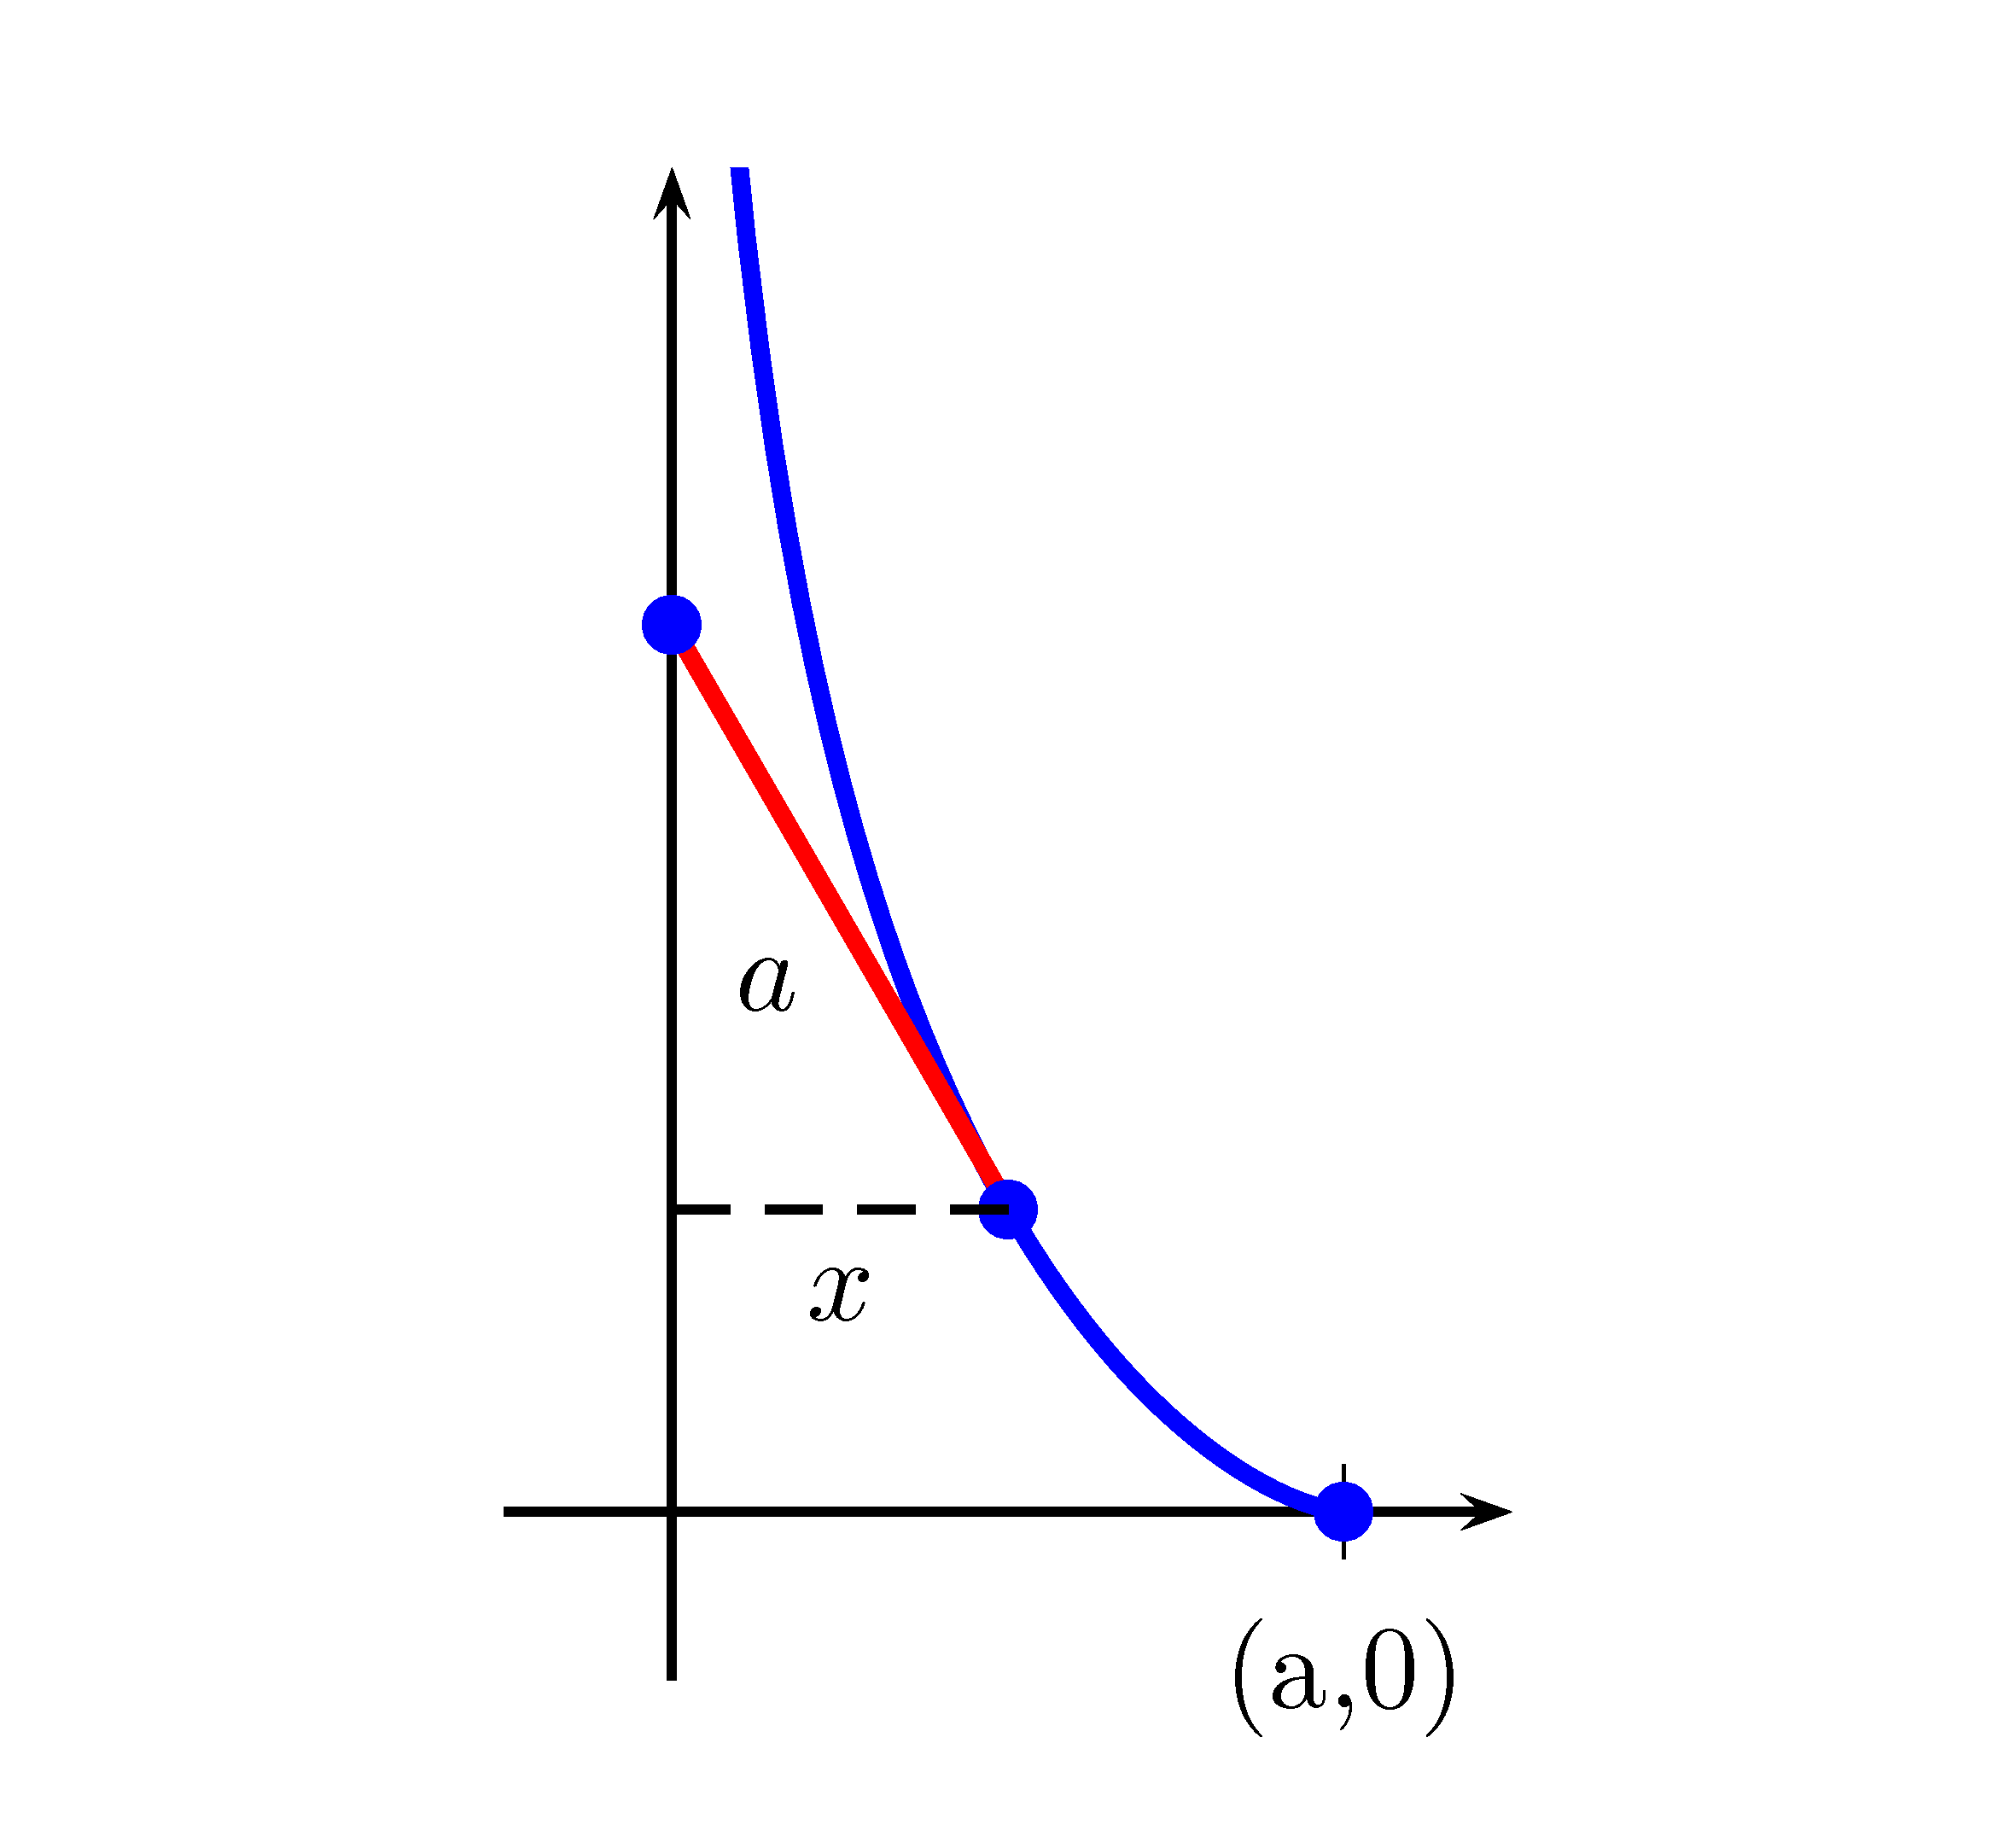
\includegraphics[width=0.75\linewidth]{resources/images/latex/tractrice} \end{center}
\vspace*{10cm}

\BeginKnitrBlock{example}
\protect\hypertarget{exm:unnamed-chunk-58}{}{\label{exm:unnamed-chunk-58}
}Trouvez les trajectoires orthogonales de la famille \(x=ky^2\).
\EndKnitrBlock{example}
\vspace*{8cm}

\BeginKnitrBlock{example}
\protect\hypertarget{exm:unnamed-chunk-59}{}{\label{exm:unnamed-chunk-59}
}Trouvez les trajectoires orthogonales de la famille \(y=ke^x\).
\EndKnitrBlock{example}
\vspace*{8cm}

\BeginKnitrBlock{example}
\protect\hypertarget{exm:parachutiste}{}{\label{exm:parachutiste} }Soit un
parachutiste qui tombe sous l'effet de la gravité avec une résistance de
l'air proportionnelle à sa vitesse. L'équation différentielle de cette
situation est : \(\dfrac{dv}{dt}+\dfrac{kv}{m}=g\) où \(m\), \(g\) et
\(k\) sont des constantes positives. Trouvez la solution de l'équation
différentielle précédente.
\EndKnitrBlock{example}
\vspace*{8cm}

\BeginKnitrBlock{example}
\protect\hypertarget{exm:unnamed-chunk-60}{}{\label{exm:unnamed-chunk-60}
}La loi de refroidissement de Newton dit que le taux de variation de la
température \(T\) d'un objet est proportionnel à la différence entre la
température de cet objet et la température ambiante (notée \(T_A\)).
Trouvez l'équation différentielle décrivant le phénomène et trouvez
\(T\) en fonction du temps.
\EndKnitrBlock{example}
\vspace*{8cm}

\hypertarget{les-equations-differentielles-lineaires}{%
\section{Les équations différentielles
linéaires}\label{les-equations-differentielles-lineaires}}

\BeginKnitrBlock{definition}[Équation différentielle linéaire]
\protect\hypertarget{def:unnamed-chunk-61}{}{\label{def:unnamed-chunk-61}
\iffalse (Équation différentielle linéaire) \fi{} }Une \textbf{équation
différentielle linéaire} est de la forme: \begin{align*}
\dfrac{dy}{dt}+P(t)y=Q(t)
\end{align*} où \(P(t)\) et \(Q(t)\) sont des fonctions qui ne doivent
dépendre que de la variable indépendante.
\EndKnitrBlock{definition}

\BeginKnitrBlock{example}
\protect\hypertarget{exm:unnamed-chunk-62}{}{\label{exm:unnamed-chunk-62}
}Voici quelques exemples d'équations différentielles linéaires:

\begin{itemize}
\tightlist
\item
  \(y'+t^2y=t^3\)
\item
  \(x^3y'-x^4y=1\) (Aprés division par \(x^2\))
\item
  \(y'=y\)
\end{itemize}
\EndKnitrBlock{example}

Pour être en mesure de résoudre ce type d'équations différentielles,
nous devrons tout d'abord utiliser une astuce.

Posons \(\mu(t)\) une fonction inconnue. Nous avons donc: \begin{align*}
\dfrac{d}{dt}[\mu y] &= \mu\dfrac{dy}{dt}+y\dfrac{d\mu}{dt} \\
&= \mu\left(Q(t)-P(t)y\right) + y\dfrac{d\mu}{dt} \qquad \text{car EDO linéaire}\\
&= \mu Q(t)-\mu P(t)y +y\dfrac{d\mu}{dt} \\
&= \mu Q(t)+y\left(\underbrace{\dfrac{d\mu}{dt}-\mu P(t)}_{\text{posons égal à 0}}\right)
\end{align*}

Ainsi: \begin{align*}
\dfrac{d}{dt}[\mu y] &= \mu Q(t) \\
\mu y &= \int \mu Q(t) \ dt\\
y &= \dfrac{1}{\mu} \int \mu Q(t) \ dt
\end{align*}

Pour pouvoir résoudre l'intégrale précédente, nous avons besoin de
connaître \(\mu\) et nous savons que: \begin{align*}
\dfrac{d\mu}{dt}-\mu P(t) &= 0 \\
\dfrac{d\mu}{dt} &= \mu P(t) \\
\int\dfrac{1}{\mu}d\mu &= \int P(t)dt \\
\ln |\mu| &= \int P(t)dt \\
\mu &= e^{\int P(t)dt}
\end{align*}

Pour résoudre une équation différentielle linéaire, il faut donc:

\begin{enumerate}
\def\labelenumi{\arabic{enumi}.}
\tightlist
\item
  Trouver \(\mu\): \(\mu = e^{\int P(t)dt}\)
\item
  Trouver \(y\): \(y = \dfrac{1}{\mu} \int \mu Q(t) \ dt\)
\end{enumerate}

\BeginKnitrBlock{example}
\protect\hypertarget{exm:unnamed-chunk-63}{}{\label{exm:unnamed-chunk-63}
}Trouvez la solution générale de \(y'+3\dfrac{y}{t}=1\).
\EndKnitrBlock{example}
\vspace*{8cm}

\BeginKnitrBlock{example}
\protect\hypertarget{exm:unnamed-chunk-64}{}{\label{exm:unnamed-chunk-64}
}Trouvez la solution générale de \(x^2y'+xy=1\) où \(x>0\) et
\(y(1)=2\).
\EndKnitrBlock{example}
\vspace*{8cm}

\BeginKnitrBlock{example}
\protect\hypertarget{exm:unnamed-chunk-65}{}{\label{exm:unnamed-chunk-65}
}Trouvez la solution générale de \(ty'+2y=t^2-t+1\).
\EndKnitrBlock{example}
\vspace*{8cm}

\BeginKnitrBlock{example}
\protect\hypertarget{exm:unnamed-chunk-66}{}{\label{exm:unnamed-chunk-66}
}Trouvez la solution générale de
\(\cos(x)y'+\sin(x)y=2\cos(x)^3\sin(x)-1\).
\EndKnitrBlock{example}
\vspace*{8cm}

\BeginKnitrBlock{example}
\protect\hypertarget{exm:unnamed-chunk-67}{}{\label{exm:unnamed-chunk-67}
}Résolvez l'équation différentielle du parachutiste, comme vu à
l'exemple \ref{exm:parachutiste}, en utilisant les équations
différentielles linéaires. L'équation différentielle est donnée par :
\(\dfrac{dv}{dt}+\dfrac{kv}{m}=g\).
\EndKnitrBlock{example}
\vspace*{8cm}

\hypertarget{problemes-de-melange}{%
\subsection{Problèmes de mélange}\label{problemes-de-melange}}

Dans des problèmes de mélange, nous cherchons \(Q(t)\) qui représente la
quantité d'une substance en fonction du temps. L'équation différentielle
de base de ce genre de problèmes est:

\begin{quote}
Taux de variation de \(Q(t)\) = Taux d'entrée de \(Q(t)\) - Taux de
sortie de \(Q(t)\)
\end{quote}

\BeginKnitrBlock{example}
\protect\hypertarget{exm:unnamed-chunk-68}{}{\label{exm:unnamed-chunk-68}
}Une cuve contient 10 L d'eau salée dans laquelle 2 kg de sel sont
dissout. De l'eau salée contenant 1 kg de sel par litre entre dans la
cuve à un débit constant de 3 L/min, et l'eau mélangée est vidée à un
taux de 4 L/min. Trouvez la quantité de sel en fonction du temps
\(Q(t)\).
\EndKnitrBlock{example}
\vspace*{10cm}

\BeginKnitrBlock{example}
\protect\hypertarget{exm:unnamed-chunk-69}{}{\label{exm:unnamed-chunk-69}
}Une cuve contient 40 L d'eau pure. De la saumure avec 3 kg de sel par
litre entre dans la cuve à un débit constant de 2 L/min, et la mixture
mélangée s'écoule à un débit constant de 3 L/min.

\begin{enumerate}
\def\labelenumi{\alph{enumi})}
\tightlist
\item
  Trouvez la quantité de sel en fonction du temps \(Q(t)\).
\item
  Quelle est la quantité de sel lorsqu'il reste 20 L dans la cuve?
\end{enumerate}
\EndKnitrBlock{example}
\vspace*{10cm}

\hypertarget{inverser-la-derivee}{%
\subsection{Inverser la dérivée}\label{inverser-la-derivee}}

Pour obtenir une équation différentielle linéaire, il faut parfois
étudier l'inverse de votre dérivée.

\begin{quote}
Plutôt que d'étudier \(\dfrac{dy}{dx}\), nous pouvons étudier
\(\dfrac{dx}{dy}\).
\end{quote}

\BeginKnitrBlock{example}
\protect\hypertarget{exm:unnamed-chunk-70}{}{\label{exm:unnamed-chunk-70}
}Trouvez la solution de l'équation différentielle
\((e^y-2xy)\dfrac{dy}{dx}=y^2\).
\EndKnitrBlock{example}
\vspace*{8cm}

\BeginKnitrBlock{example}
\protect\hypertarget{exm:unnamed-chunk-71}{}{\label{exm:unnamed-chunk-71}
}Trouvez les familles de courbes orthogonales à \(y^2=ce^x+x+1\) où
\(c\in\mathbb{R}\).
\EndKnitrBlock{example}
\vspace*{8cm}

\hypertarget{les-equations-differentielles-a-coefficients-constants-dordre-2}{%
\section{Les équations différentielles à coefficients constants d'ordre
2}\label{les-equations-differentielles-a-coefficients-constants-dordre-2}}

\hypertarget{quelques-rappels-concernant-les-nombres-complexes}{%
\subsection{Quelques rappels concernant les nombres
complexes}\label{quelques-rappels-concernant-les-nombres-complexes}}

\BeginKnitrBlock{definition}[Nombre complexe]
\protect\hypertarget{def:unnamed-chunk-72}{}{\label{def:unnamed-chunk-72}
\iffalse (Nombre complexe) \fi{} }Un nombre complexe \(z\) s'écrit sous
la forme \(z=a+bi\), où \(a,b \in \mathbb{R}\) et tel que \(i^2=-1\).

Nous disons que \(a\) est la partie réelle de \(z\) et \(b\) est la
partie imaginaire de \(z\).

L'ensemble des nombres complexes est noté \(\mathbb{C}\).

Nous pouvons également écrire \(z\) sous une form dite polaire qui est
\(z=r(\cos(\theta)+i\sin(\theta))\), où \(r=\sqrt{a^2+b^2}\) et
\(\theta=\text{Arctan}\left(\dfrac{b}{a}\right)\).
\EndKnitrBlock{definition}

La figure \ref{fig:nombrescomplexes} permet de représenter un nombre
complexe de façon géométrique.

\begin{figure}

{\centering 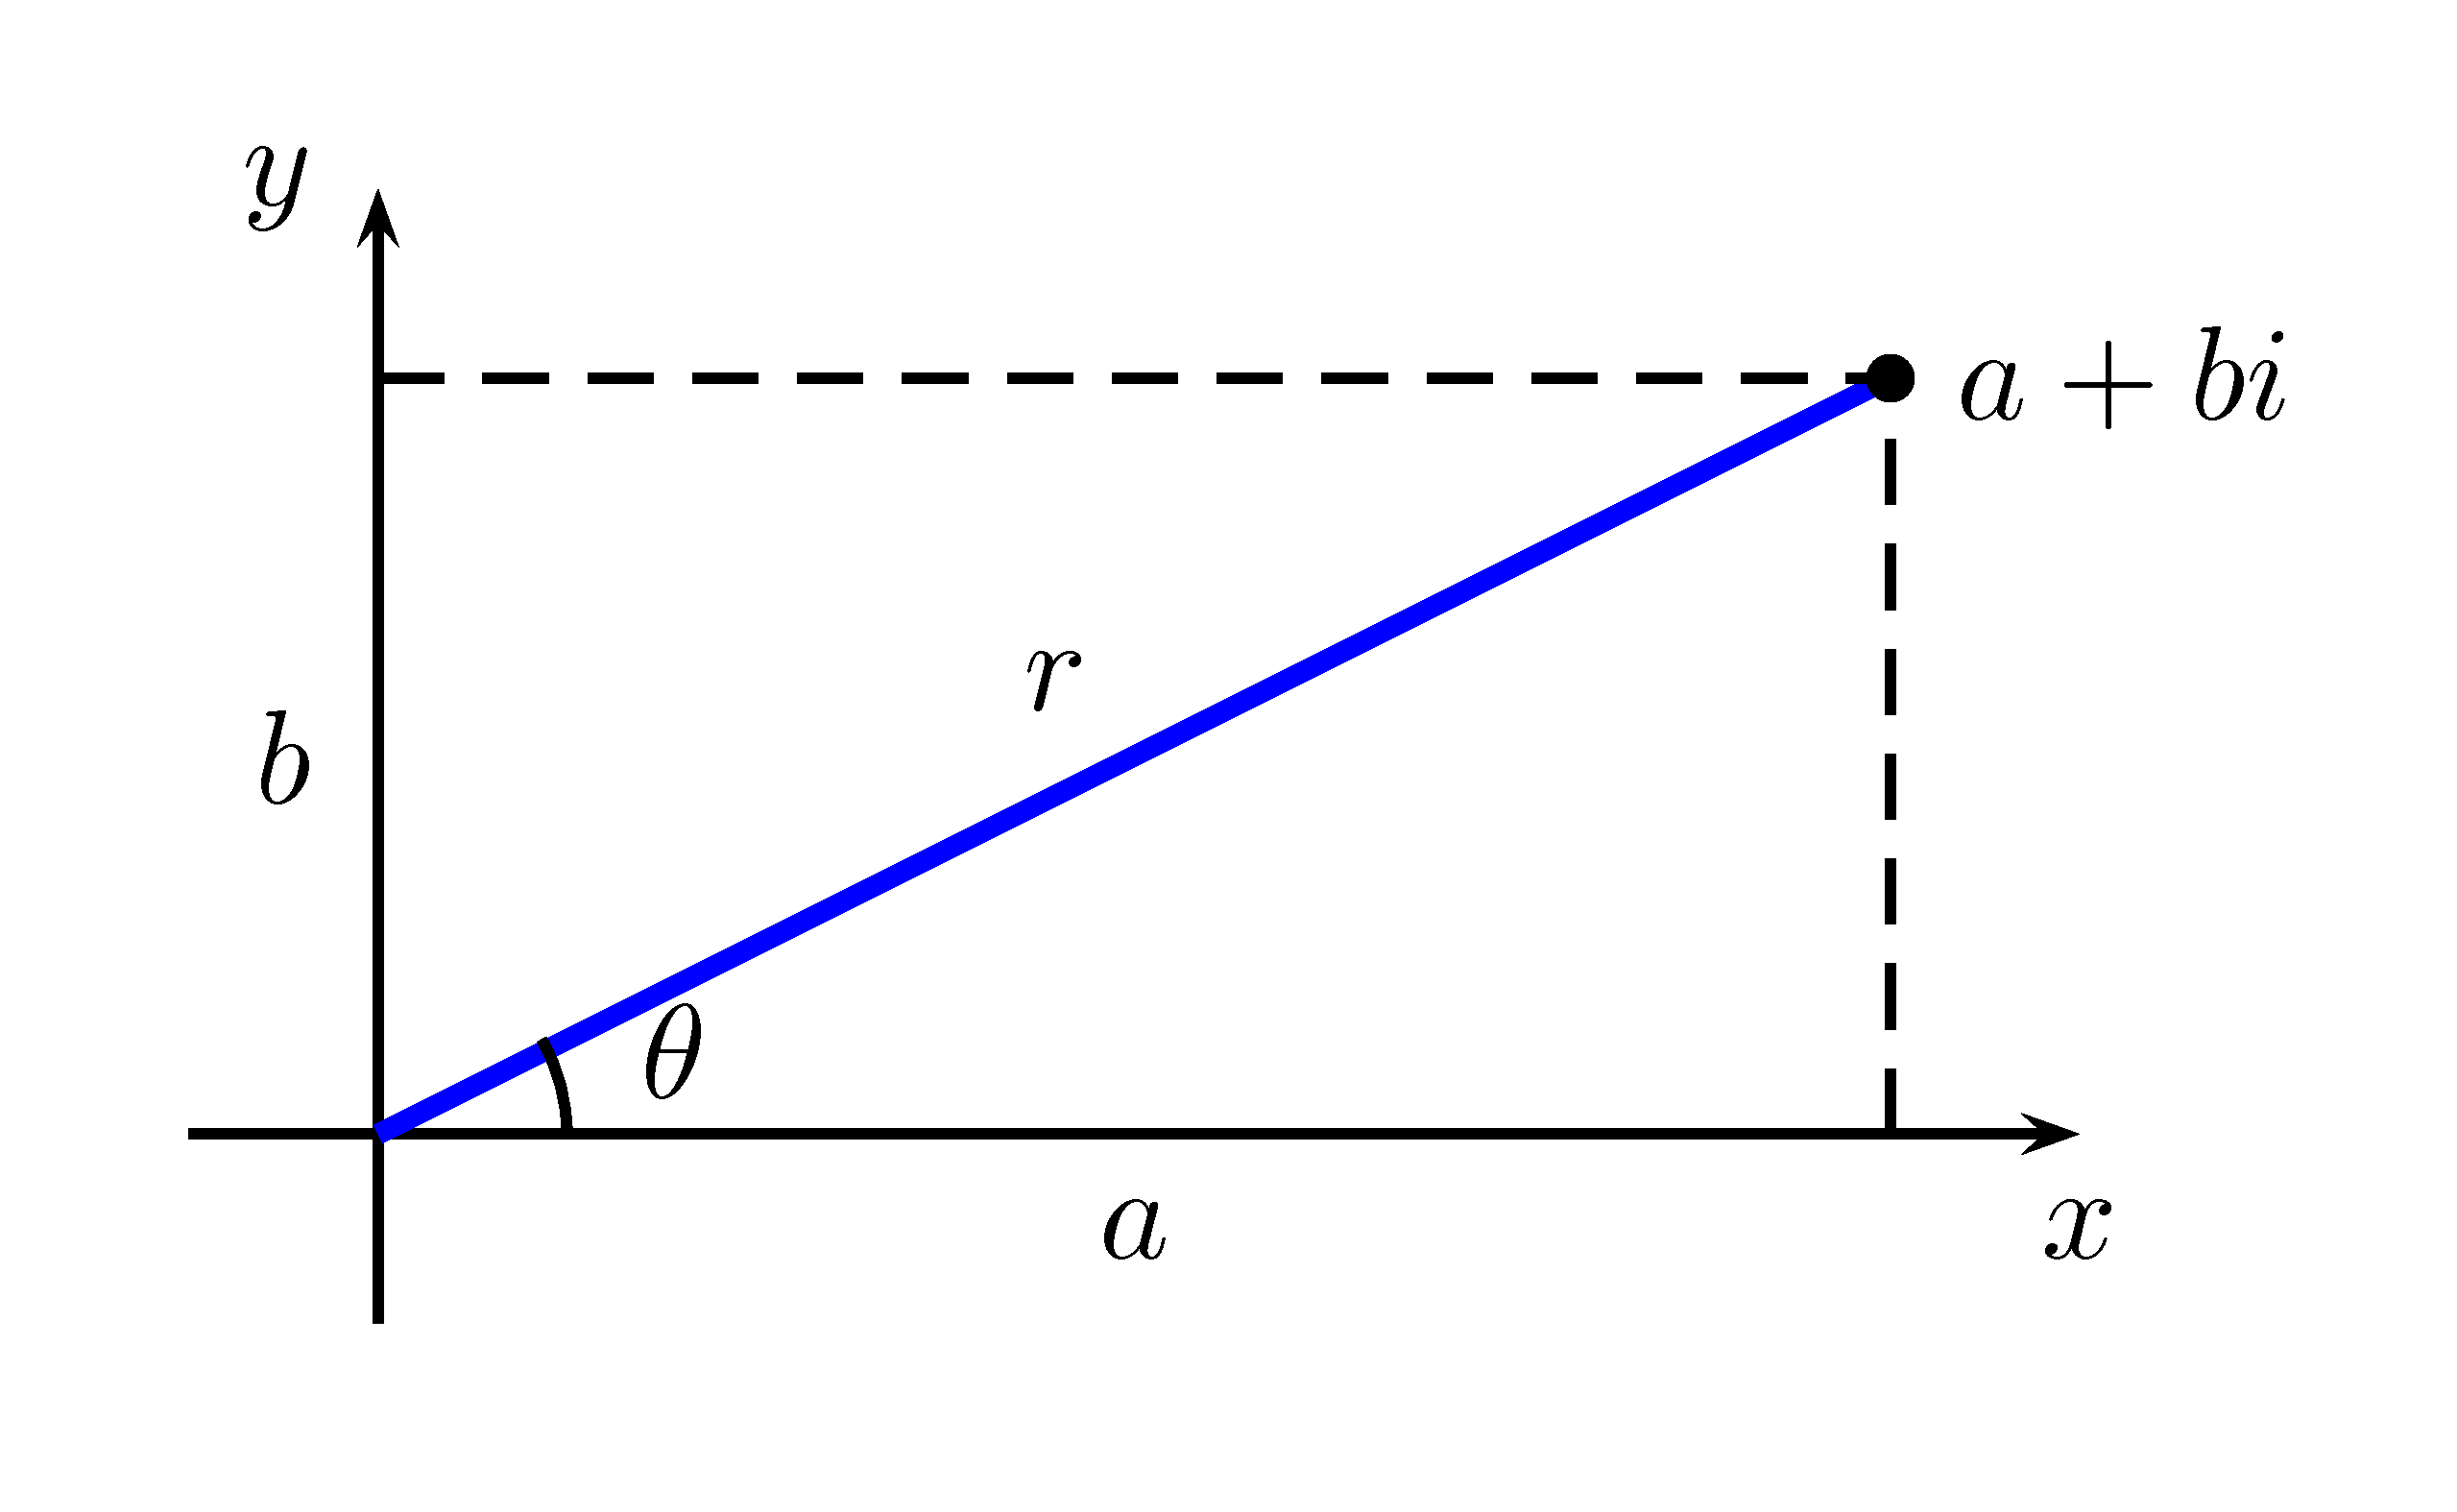
\includegraphics[width=0.5\linewidth]{resources/images/latex/nombrescomplexes} 

}

\caption{Représentation d'un nombre complexe}\label{fig:nombrescomplexes}
\end{figure}

\BeginKnitrBlock{theorem}[L'identité d'Euler]
\protect\hypertarget{thm:identite-euler}{}{\label{thm:identite-euler}
\iffalse (L'identité d'Euler) \fi{} }Soit le nombre complexe écrit sous
la forme \(z=r(\cos(\theta)+i\sin(\theta))\). Alors ce nombre peut
s'écrire de la manière suivante: \(z=re^{i\theta}\).
\EndKnitrBlock{theorem}

\BeginKnitrBlock{proof}
\iffalse{} {Preuve. } \fi{}La démonstration est laissée à l'étudiante ou
l'étudiant. \textbf{Astuce}: Il faut utiliser les séries de MacLaurin de
\(e^x\), \(\sin(x)\) et \(\cos(x)\).
\EndKnitrBlock{proof}

\BeginKnitrBlock{corollary}
\protect\hypertarget{cor:sin-cos-ei}{}{\label{cor:sin-cos-ei} }Nous avons:
\begin{align*}
\cos(\theta) &= \dfrac{e^{i\theta}+e^{-i\theta}}{2} \\
\sin(\theta) &= \dfrac{e^{i\theta}-e^{-i\theta}}{2i}
\end{align*}
\EndKnitrBlock{corollary}

\BeginKnitrBlock{proof}
\iffalse{} {Preuve. } \fi{}Pour démontrer ce résultat, nous utiliserons
le théorème \ref{thm:identite-euler}. Nous avons: \begin{align}
e^{i\theta} &= \cos(\theta)+i\sin(\theta)\label{eq:eplus} \\
e^{-i\theta} &= \cos(-\theta)+i\sin(-\theta) \notag \\
&= \cos(\theta)-i\sin(\theta)\label{eq:emoins}
\end{align}

Si nous additions les équations \eqref{eq:eplus} et \eqref{eq:emoins}:
\begin{align*}
e^{i\theta}+e^{-i\theta} &= \cos(\theta)+i\sin(\theta)+\cos(\theta)-i\sin(\theta) \\
&= 2\cos(\theta) \\
\cos(\theta) &= \dfrac{e^{i\theta}+e^{-i\theta}}{2}
\end{align*}

Si nous faisons la différence entre les équations \eqref{eq:eplus} et
\eqref{eq:emoins}: \begin{align*}
e^{i\theta}-e^{-i\theta} &= \cos(\theta)+i\sin(\theta)-(\cos(\theta)-i\sin(\theta)) \\
&= 2i\sin(\theta) \\
\sin(\theta) &= \dfrac{e^{i\theta}-e^{-i\theta}}{2i}
\end{align*}
\EndKnitrBlock{proof}

\hypertarget{les-equations-differentielles-homogenes-a-coefficients-constants-dordre-2}{%
\subsection{Les équations différentielles homogènes à coefficients
constants d'ordre
2}\label{les-equations-differentielles-homogenes-a-coefficients-constants-dordre-2}}

\BeginKnitrBlock{definition}[Équation différentielle homogène à coefficients constants d'ordre 2]
\protect\hypertarget{def:unnamed-chunk-75}{}{\label{def:unnamed-chunk-75}
\iffalse (Équation différentielle homogène à coefficients constants
d'ordre 2) \fi{} }Une \textbf{équation différentielle homogène à
coefficients constants d'ordre 2} est une équation différentielle de la
forme: \begin{align}
a\dfrac{d^2y}{dx^2}+b\dfrac{dy}{dx}+cy &= 0 \label{eq:homogene2}
\end{align} où \(a,b,c \in \mathbb{R}\) et \(a\neq 0\).
\EndKnitrBlock{definition}

\begin{quote}
Le terme \emph{homogène} indique que le membre de droite de l'équation
\eqref{eq:homogene2} est nul. Nous traiterons le cas à la section
\ref{non-homogene-2}.
\end{quote}

Avant de résoudre ce type d'équations différentielles, la prochaine
proposition sera cruciale.

\BeginKnitrBlock{proposition}
\protect\hypertarget{prp:combinaison-lineaire-solution}{}{\label{prp:combinaison-lineaire-solution}
}Si \(y_1(x)\) et \(y_2(x)\) sont deux solutions de l'équation
\eqref{eq:homogene2}, alors \(y(x)=C_1y_1(x)+C_2y_2(x)\), où
\(C_1,C_2\in\mathbb{R}\), est aussi une solution de l'équation
\eqref{eq:homogene2}.
\EndKnitrBlock{proposition}

\BeginKnitrBlock{proof}
\iffalse{} {Preuve. } \fi{}Nous avons que: \begin{align*}
ay_1''+by_1'+cy_1 &= 0 \\
ay_2''+by_2'+cy_2 &= 0
\end{align*} car \(y_1\) et \(y_2\) sont des solutions de
\eqref{eq:homogene2}. Nous avons que: \begin{align*}
y &= C_1y_1+C_2y_2 \\
y' &= C_1y_1'+C_2y_2' \\
y'' &= C_1y_1''+C_2y_2'' \\
\end{align*} Ainsi: \begin{align*}
ay''+by'+cy &= a(C_1y_1''+C_2y_2'')+b(C_1y_1'+C_2y_2')+c(C_1y_1+C_2y_2) \\
&= C_1\underbrace{(ay_1''+by_1'+cy_1)}_{=\ 0}+C_2\underbrace{(ay_2''+by_2'+cy_2)}_{=\ 0} \\
&= 0
\end{align*}
\EndKnitrBlock{proof}

\begin{quote}
Une combinaison linéaire de solutions est aussi une solution.
\end{quote}

Nous pouvons maintenant résoudre l'équation \eqref{eq:homogene2} en
supposant que la solution est de la forme \(y=e^{rx}\), où \(r\) est une
constante qu'il nous reste à déterminer.

\begin{quote}
Pour résoudre une équation différentielle homogène d'ordre 2 à
coefficients constants, il faut toujours poser la solution \(y=e^{rx}\).
\end{quote}

Nous avons donc: \begin{align*}
y &= e^{rx} \\
y' &= re^{rx} \\
y'' &= r^2e^{rx}
\end{align*}

Nous substituons ces résultats dans l'équation \eqref{eq:homogene2}:
\begin{align}
a\dfrac{d^2y}{dx^2}+b\dfrac{dy}{dx}+cy &= 0 \notag \\
ar^2e^{rx}+bre^{rx}+ce^{rx} &= 0 \notag \\
e^{rx}(ar^2+br+c) &= 0 \notag \\
ar^2+br+c &= 0\label{eq:quadratique}
\end{align}

L'équation \eqref{eq:quadratique} se nomme polynôme caractéristique de
l'équation \eqref{eq:homogene2}. Déterminer les valeurs de \(r\) revient à
trouver les racines du polynôme caractéristique et donc: \begin{align*}
r_{1,2} &= \dfrac{-b\pm\sqrt{b^2-4ac}}{2a}
\end{align*} Nous devrons étudier trois cas distincts qui dépendent du
discriminant \(b^2-4ac\).

\hypertarget{cas-1-b2-4ac0}{%
\subsubsection{\texorpdfstring{Cas 1:
\(b^2-4ac>0\)}{Cas 1: b\^{}2-4ac\textgreater{}0}}\label{cas-1-b2-4ac0}}

Dans ce cas, le polynôme caractéristique fournit deux valeurs de \(r\)
\textbf{réelles}, que nous notons \(r_1\) et \(r_2\). Nous avons donc
\(y_1(x)=e^{r_1x}\) qui est une solution de \eqref{eq:homogene2} et
également \(y_2=e^{r_2x}\). Par la proposition
\ref{prp:combinaison-lineaire-solution}, nous obtenons la solution
générale: \begin{align*}
y(x) &= C_1e^{r_1x}+C_2e^{r_2x}
\end{align*} où \(C_1,C_2\in\mathbb{R}\).

\BeginKnitrBlock{example}
\protect\hypertarget{exm:unnamed-chunk-77}{}{\label{exm:unnamed-chunk-77}
}Résolvez l'équation différentielle \(y''+y'-6y=0\) avec comme
conditions initiales \(y(0)=0\) et \(y'(0)=1\).
\EndKnitrBlock{example}
\vspace*{10cm}

\hypertarget{cas-2-b2-4ac0}{%
\subsubsection{\texorpdfstring{Cas 2:
\(b^2-4ac<0\)}{Cas 2: b\^{}2-4ac\textless{}0}}\label{cas-2-b2-4ac0}}

Dans ce cas, le polynôme caractéristique fournit deux valeurs de \(r\)
\textbf{complexes}. Posons \(\gamma=-\dfrac{b}{2a}\) et
\(\omega=\dfrac{\sqrt{4ac-b^2}}{2a}\) ce qui implique que
\(r_1=\gamma+\omega i\) et \(r_2=\gamma -\omega i\). Nous avons donc
deux solutions à l'équation \eqref{eq:homogene2}, soit
\(y_1=e^{r_1x}=e^{(\gamma+\omega i)x}\) et
\(y_2=e^{r_2x}=e^{(\gamma-\omega i)x}\).

Puisque les solutions précédentes sont complexes, nous allons utiliser
la proposition \ref{prp:combinaison-lineaire-solution} et le corollaire
\ref{cor:sin-cos-ei} pour créer deux nouvelles solutions réelles:
\begin{align*}
y_3(x) &= \dfrac{y_1(x)+y_2(x)}{2} \\
&= \dfrac{e^{(\gamma+\omega i)x}+e^{(\gamma-\omega i)x}}{2} \\
&= e^{\gamma x}\left( \dfrac{e^{\omega i x}+e^{-\omega i x}}{2} \right) \\
&= e^{\gamma x}\cos(\omega x) \\
y_4(x) &= \dfrac{y_1(x)-y_2(x)}{2i} \\
&= \dfrac{e^{(\gamma+\omega i)x}-e^{(\gamma-\omega i)x}}{2i} \\
&= e^{\gamma x}\left( \dfrac{e^{\omega i x}-e^{-\omega i x}}{2i} \right) \\
&= e^{\gamma x}\sin(\omega x)
\end{align*}

D'où la solution générale de l'équation \eqref{eq:homogene2} est:
\begin{align*}
y(x) &= e^{\gamma x}\left( C_1\cos(\omega x)+C_2\sin(\omega x) \right)
\end{align*}

\BeginKnitrBlock{example}
\protect\hypertarget{exm:unnamed-chunk-78}{}{\label{exm:unnamed-chunk-78}
}Trouvez la solution de l'équation différentielle \(y''+2y'+10y=0\)
ayant comme conditions initiales \(y(0)=0\) et \(y'(0)=3\).
\EndKnitrBlock{example}
\vspace*{10cm}

\hypertarget{cas-3-b2-4ac0}{%
\subsubsection{\texorpdfstring{Cas 3:
\(b^2-4ac=0\)}{Cas 3: b\^{}2-4ac=0}}\label{cas-3-b2-4ac0}}

Dans ce cas, nous n'obtenons qu'une seule valeur de
\(r=-\dfrac{b}{2a}\). Puisque nous n'avons qu'une seule solution, nous
devons en trouver une autre pour être en mesure de construire une
combinaison linéaire. Nous allons démontrer que \(y_2(x)=xe^{rx}\) est
aussi une solution de l'équation différentielle \eqref{eq:homogene2}.
\BeginKnitrBlock{proof}
\iffalse{} {Preuve. } \fi{}\begin{align*}
y_2 &= xe^{rx} \\
y_2' &= e^{rx}+rxe^{rx} \\
y_2'' &= re^{rx}+re^{rx}+r^2xe^{rx}
\end{align*} Et donc: \begin{align*}
ay'' +by' +cy &= 0 \\
a(2re^{rx}+r^2xe^{rx})+b(e^{rx}+rxe^{rx})+c(xe^{rx}) &= 0 \\
e^{rx}(2ar+ar^2x+b+brx+cx) &= 0 \\
e^{rx}(\underbrace{(ar^2+br+c)}_{=0}x+\underbrace{(2ar+b)}_{=0}) &= 0 
\end{align*}
\EndKnitrBlock{proof}

La solution générale est donc de la forme: \begin{align*}
y(x) &= C_1e^{rx}+C_2xe^{rx}
\end{align*}

\BeginKnitrBlock{example}
\protect\hypertarget{exm:unnamed-chunk-80}{}{\label{exm:unnamed-chunk-80}
}Trouvez la solution de l'équation différentielle \(y''+2y'+y=0\).
\EndKnitrBlock{example}
\vspace*{5cm}

\BeginKnitrBlock{example}
\protect\hypertarget{exm:unnamed-chunk-81}{}{\label{exm:unnamed-chunk-81}
}Trouvez les solutions des équations différentielles suivantes:

\begin{enumerate}
\def\labelenumi{\alph{enumi})}
\tightlist
\item
  \(y''-9y'+20y=0\)
\item
  \(2y''-4y'+8y=0\)
\item
  \(y''+6y'+9=0\)
\end{enumerate}
\EndKnitrBlock{example}
\vspace*{20cm}

\hypertarget{non-homogene-2}{%
\subsection{Les équations différentielles non homogènes à coefficients
constants d'ordre 2}\label{non-homogene-2}}

\BeginKnitrBlock{definition}[Équation différentielle non homogène à coefficients constants d'ordre 2]
\protect\hypertarget{def:unnamed-chunk-82}{}{\label{def:unnamed-chunk-82}
\iffalse (Équation différentielle non homogène à coefficients constants
d'ordre 2) \fi{} }Une \textbf{équation différentielle non homogène à
coefficients constants d'ordre 2} est une équation différentielle de la
forme: \begin{align}
a\dfrac{d^2y}{dx^2}+b\dfrac{dy}{dx}+cy &= F(x) \label{eq:nonhomogene2}
\end{align} où \(a,b,c \in \mathbb{R}\) et \(a\neq 0\). De plus \(F(x)\)
est une fonction qui ne dépend que de la variable indépendante.
\EndKnitrBlock{definition}

Pour résoudre ce type d'équations différentielles, nous aurons besoin du
théorème suivant:

\BeginKnitrBlock{theorem}
\protect\hypertarget{thm:unnamed-chunk-83}{}{\label{thm:unnamed-chunk-83}
}Soit une équation différentielle de la forme: \begin{align*}
a\dfrac{d^2y}{dx^2}+b\dfrac{dy}{dx}+cy &= F(x)
\end{align*} La solution de cette équation différentielle est de la
forme: \begin{align*}
y(x) &= C_1y_1(x)+C_2y_2(x)+y_p
\end{align*} où \(y_1\) et \(y_2\) sont les solutions de l'équation
homogène associée à l'équation \eqref{eq:nonhomogene2}, c'est-à-dire:
\begin{align*}
a\dfrac{d^2y}{dx^2}+b\dfrac{dy}{dx}+cy &= 0
\end{align*} et \(y_p\) est une solution particulière de l'équation non
homogène.
\EndKnitrBlock{theorem}

\BeginKnitrBlock{proof}
\iffalse{} {Preuve. } \fi{}La démonstration est laissée à l'étudiante ou
à l'étudiant.
\EndKnitrBlock{proof}

Nous verrons deux méthodes pour trouver \(y_p\).

\hypertarget{la-methode-des-coefficients-indetermines}{%
\subsubsection{La méthode des coefficients
indéterminés}\label{la-methode-des-coefficients-indetermines}}

Cette méthode consiste à étudier la nature de la fonction \(F(x)\) et à
supposer que \(y_p\) est de même nature. La table
\ref{tab:coeff-indetermines} montre la forme de la solution particulière
\(y_p\) selon la nature de \(F(x)\).

\begin{longtable}[]{@{}cc@{}}
\caption{\label{tab:coeff-indetermines} Les diverses formes de coefficients
indéterminés.}\tabularnewline
\toprule
\begin{minipage}[b]{0.55\columnwidth}\centering
Forme de \(F(x)\)\strut
\end{minipage} & \begin{minipage}[b]{0.39\columnwidth}\centering
Forme de \(y_p\)\strut
\end{minipage}\tabularnewline
\midrule
\endfirsthead
\toprule
\begin{minipage}[b]{0.55\columnwidth}\centering
Forme de \(F(x)\)\strut
\end{minipage} & \begin{minipage}[b]{0.39\columnwidth}\centering
Forme de \(y_p\)\strut
\end{minipage}\tabularnewline
\midrule
\endhead
\begin{minipage}[t]{0.55\columnwidth}\centering
Polynôme de degré \(n\)\strut
\end{minipage} & \begin{minipage}[t]{0.39\columnwidth}\centering
\(y_p=a_nx^n+a_{n-1}x^{n-1}+\ldots+a_x+a_0\)\strut
\end{minipage}\tabularnewline
\begin{minipage}[t]{0.55\columnwidth}\centering
\(F(x)\) possède un \(\sin(\omega x)\) et/ou un \(\cos(\omega x)\)\strut
\end{minipage} & \begin{minipage}[t]{0.39\columnwidth}\centering
\(y_p=A\cos(\omega x)+B\sin(\omega x)\)\strut
\end{minipage}\tabularnewline
\begin{minipage}[t]{0.55\columnwidth}\centering
\(F(x)\) possède une exponentielle \(e^{\alpha x}\)\strut
\end{minipage} & \begin{minipage}[t]{0.39\columnwidth}\centering
\(y_p=A^{\alpha x}\)\strut
\end{minipage}\tabularnewline
\bottomrule
\end{longtable}

\BeginKnitrBlock{example}
\protect\hypertarget{exm:unnamed-chunk-85}{}{\label{exm:unnamed-chunk-85}
}Trouvez la solution générale de l'équation différentielle
\(y''+y'-6y=3x^2\).
\EndKnitrBlock{example}
\vspace*{10cm}

\BeginKnitrBlock{example}
\protect\hypertarget{exm:unnamed-chunk-86}{}{\label{exm:unnamed-chunk-86}
}Trouvez la solution générale de l'équation différentielle
\(y''+y'-6y=e^{4x}+\cos(3x)\).
\EndKnitrBlock{example}
\vspace*{10cm}

\BeginKnitrBlock{example}
\protect\hypertarget{exm:unnamed-chunk-87}{}{\label{exm:unnamed-chunk-87}
}Trouvez la solution générale de l'équation différentielle
\(y''+2y'+10y=\cos(2t)\) avec les conditions intiales
\(y(0)=-\frac{1}{2}\) et \(y'(0)=4\).
\EndKnitrBlock{example}
\vspace*{15cm}

\hypertarget{la-methode-de-variation-des-parametres-ou-methode-de-lagrange}{%
\subsubsection{La méthode de variation des paramètres (ou méthode de
Lagrange)}\label{la-methode-de-variation-des-parametres-ou-methode-de-lagrange}}

La méthode de variation des paramètres est souvent plus longue à
utiliser que la méthode des coefficients indéterminés, par contre, elle
est valide pour tous les types de fonctions \(F(x)\).

Nous débutons en trouvant les solutions \(y_1\) et \(y_2\) de l'équation
différentielle homogène associée à l'équation: \begin{align*}
ay''+by'+cy=F(x)
\end{align*}

Supposons que la solution est de la forme : \begin{align*}
y(x) &= \mu_1(x)y_1(x)+\mu_2(x)y_2(x)
\end{align*} Afin d'alléger la notation, nous omettrons la dépendance en
\(x\). Nous cherchons donc \(\mu_1\) et \(\mu_2\). Avant de substituer
dans l'équation différentielle, nous allons trouver les dérivées
successives de \(y\). \begin{align*}
y' &= \mu_1y_1'+\mu_1'y_1+\mu_2'y_2+\mu_2y_2'
\end{align*} Nous allons maintenant faire la supposition que
\(\mu_1'y_1+\mu_2'y_2=0\) et donc: \begin{align*}
y' &= \mu_1y_1'+\mu_2y_2'
\end{align*} Trouvons maintenant la dérivée seconde: \begin{align*}
y' &= \mu_1'y_1'+\mu_1y_1''+\mu_2'y_2'+\mu_2y_2''
\end{align*} Nous avons donc: \begin{align*}
ay''+by'+cy &= F(x) \\
a(\mu_1'y_1'+\mu_1y_1''+\mu_2'y_2'+\mu_2y_2'')+b(\mu_1y_1'+\mu_2y_2')+c(\mu_1y_1+\mu_2y_2) &= F(x) \\
\mu_1\underbrace{(ay_1''+by_1'+cy_1)}_{=0}+\mu_2\underbrace{(ay_2''+by_2'+cy_2)}_{=0}+\mu_1'y_1'+\mu_2'y_2' &= F(x) \\
\mu_1'y_1'+\mu_2'y_2' &= F(x)
\end{align*} Ainsi, pour déterminer \(\mu_1\) et \(\mu_2\), nous avons
les deux équations suivantes: \begin{align*}
\mu_1'y_1+\mu_2'y_2 &= 0 \\
\mu_1'y_1'+\mu_2'y_2' &= F(x)
\end{align*} Nous pouvons utiliser la méthode de Cramer pour résoudre ce
système d'équations linéaires: \begin{align*}
\mu_1'&= \dfrac{
\begin{vmatrix}
0&y_2\\
F(x)&y_2'
\end{vmatrix}}{
\begin{vmatrix}
y_1 &y_2\\
y_1'&y_2'
\end{vmatrix}
}=-\dfrac{y_2F(x)}{W(y_1,y_2)}\\
\mu_2'&= \dfrac{
\begin{vmatrix}
y_1&0\\
y_1'&F(x)
\end{vmatrix}}{
\begin{vmatrix}
y_1 &y_2\\
y_1'&y_2'
\end{vmatrix}
}=\dfrac{y_1F(x)}{W(y_1,y_2)}
\end{align*}

\BeginKnitrBlock{definition}[Wronskien]
\protect\hypertarget{def:unnamed-chunk-88}{}{\label{def:unnamed-chunk-88}
\iffalse (Wronskien) \fi{} }Nous appelons le \textbf{Wronskien} de deux
fonctions \(y_1\) et \(y_2\), le résultat suivant: \begin{align*}
W(y_1,y_2)=\begin{vmatrix}
y_1 &y_2\\
y_1'&y_2'
\end{vmatrix}
\end{align*}
\EndKnitrBlock{definition}

\BeginKnitrBlock{remark}
\iffalse{} {Remarque. } \fi{}Le \textbf{Wronskien} n'est jamais égal à
zéro lorsque nous résolvons une équation différentielle car \(y_1\) et
\(y_2\) sont choisies pour être linéairement indépendantes.
\EndKnitrBlock{remark}

Nous pouvons maintenant trouver nos deux fonctions \(\mu_1\) et
\(\mu_2\): \begin{align*}
\mu_1&=-\int \dfrac{y_2(x)F(x)}{W(y_1,y_2)}dx\\
\mu_2&=\int \dfrac{y_1(x)F(x)}{W(y_1,y_2)}dx
\end{align*}

\BeginKnitrBlock{example}
\protect\hypertarget{exm:unnamed-chunk-90}{}{\label{exm:unnamed-chunk-90}
}Trouvez la solution particulière de l'équation différentielle
\(y''+y=\csc(x)\).
\EndKnitrBlock{example}
\vspace*{10cm}

\BeginKnitrBlock{example}
\protect\hypertarget{exm:unnamed-chunk-91}{}{\label{exm:unnamed-chunk-91}
}Trouvez les solutions des équations différentielles suivantes en
utilisant les deux méthodes:

\begin{itemize}
\tightlist
\item
  Méthode des coefficients indéterminés
\item
  Méthode de variation des paramètres
\end{itemize}

\begin{enumerate}
\def\labelenumi{\alph{enumi}.}
\tightlist
\item
  \(y''-2y'+y=2x\)
\item
  \(y''-y'-6y=e^{-x}\)
\end{enumerate}
\EndKnitrBlock{example}

\hypertarget{applications-des-equations-differentielles-du-deuxieme-ordre-a-coefficients-constants}{%
\section{Applications des équations différentielles du deuxième ordre à
coefficients
constants}\label{applications-des-equations-differentielles-du-deuxieme-ordre-a-coefficients-constants}}

Nous discuterons en particulier de l'oscillateur harmonique forcé.

\BeginKnitrBlock{example}[Oscillateur harmonique forcé]
\protect\hypertarget{exm:unnamed-chunk-92}{}{\label{exm:unnamed-chunk-92}
\iffalse (Oscillateur harmonique forcé) \fi{} }Soit un ressort de
constante \(k\) auquel nous attachons une masse \(M\). Si le frottement
est proportionnel à la vitesse de la masse et que celle-ci subit une
force périodique, nous pouvons décrire le mouvement avec l'équation
suivante: \begin{align*}
\dfrac{d^2x}{dt^2}+\dfrac{c}{M}\dfrac{dx}{dt}+\dfrac{k}{M}x &= \dfrac{F_0}{M}\cos(\omega t)
\end{align*} Nous pouvons réécrire l'équation précédente en introduisant
les variables \(b=\dfrac{c}{2M}\) et \(a=\sqrt{\dfrac{k}{M}}\):
\begin{align*}
\dfrac{d^2x}{dt^2}+2b\dfrac{dx}{dt}+a^2x &= \dfrac{F_0}{M}\cos(\omega t)
\end{align*} Ce changement nous simplifiera le travail.

\begin{enumerate}
\def\labelenumi{\alph{enumi}.}
\tightlist
\item
  Trouvez la solution homogène de l'équation différentielle.
\item
  Supposez que \(b=0\), c'est-à-dire qu'il n'y a pas de frottement.
  Trouvez la solution particulière dans le cas où \(a\neq \omega\).
  (Vous étudiez dans ce cas la situation des \textbf{battements}). Pour
  en savoir plus sur le phénomène de
  \href{https://fr.wikipedia.org/wiki/Battement_(physique)}{battements}.
\item
  Supposez que \(b=0\), c'est-à-dire qu'il n'y a pas de frottement.
  Trouvez la solution particulière dans le cas où \(a =\omega\). (Vous
  étudiez dans ce cas la situation de \textbf{résonnance}) Pour voir en
  action le phénomène de résonnance,
  \href{https://www.youtube.com/watch?v=j-zczJXSxnw}{Tacoma Narrows
  Bridge} .
\end{enumerate}
\EndKnitrBlock{example}

\hypertarget{geogebra-equations-diff}{%
\section{GeoGebra}\label{geogebra-equations-diff}}

\hypertarget{applet_container}{}

\newpage

\hypertarget{pages-supplementaires-1}{%
\section{Pages supplémentaires}\label{pages-supplementaires-1}}

Des pages blanches supplémentaires pour ajouter, potentiellement, de
nouveaux exemples et exercices.

\multido{\i=1+1}{4}{
\newpage
\mbox{}
}

\hypertarget{coordpolaires}{%
\chapter{Les coordonnées polaires}\label{coordpolaires}}

Vous trouverez à la section \ref{geogebra-polaire} une application
\href{https://www.geogebra.org/?lang=fr}{GeoGebra} vous permettant de
visualiser des courbes en coordonnées polaires. À noter que cette
application n'est disponible que dans la version en ligne de ce
document.

\hypertarget{introduction-2}{%
\section{Introduction}\label{introduction-2}}

Les coordonnées polaires sont un autre système pour décrire un point
\(P\) de \(\mathbb{R}^2\). Les coordonnées cartésiennes associent à
chaque point \(P\) un couple \((x,y)\). Les coordonnées polaires
consistent à décrire ce point \(P\) avec le couple \((r,\theta)\), où
\(r\) est la longueur du segment de droite reliant l'origine au point
\(P\) et \(\theta\) est l'angle entre ce segment de droite et l'axe des
\(x\) positifs. La figure \ref{fig:coordpolaires} représente ce type de
coordonnées.

\begin{figure}

{\centering 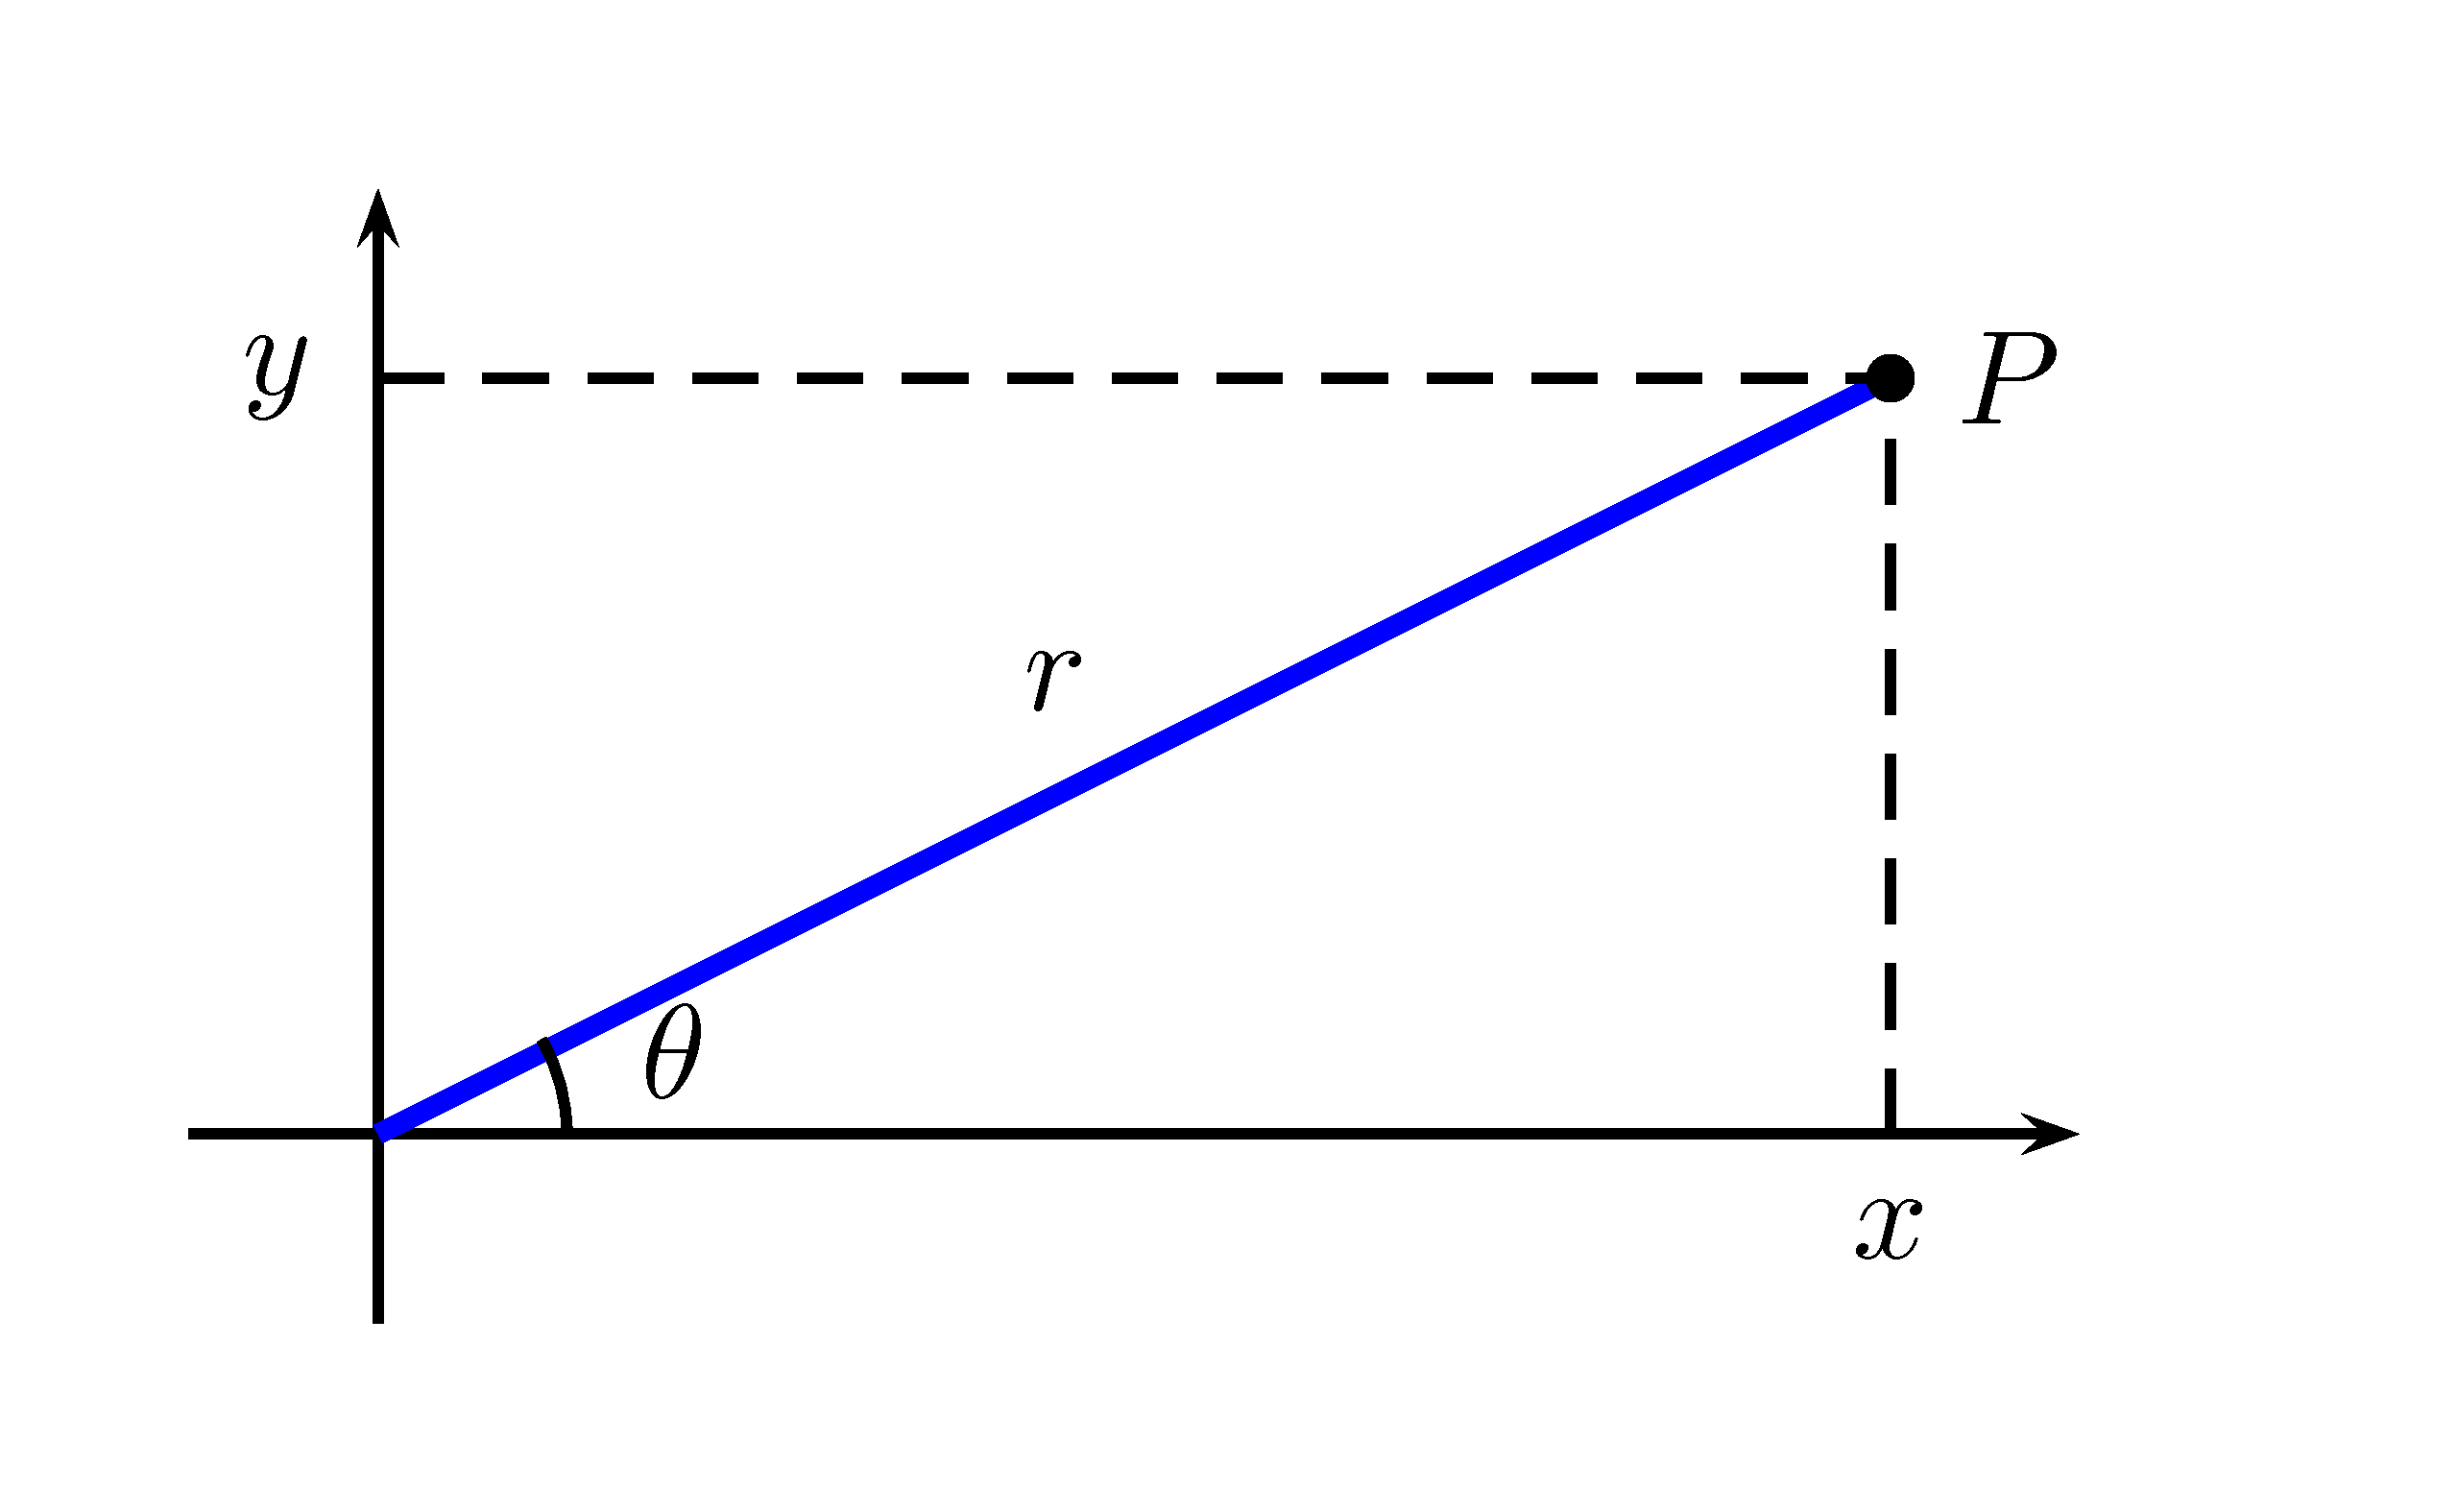
\includegraphics[width=0.5\linewidth]{resources/images/latex/coordpolaires} 

}

\caption{Coordonnées polaires d'un point $P$}\label{fig:coordpolaires}
\end{figure}

Il est primordial de pouvoir convertir les coordonnées cartésiennes à
des coordonnées polaires et vice-versa.

\BeginKnitrBlock{proposition}[Coordonnées cartésiennes à coordonnées polaires]
\protect\hypertarget{prp:unnamed-chunk-93}{}{\label{prp:unnamed-chunk-93}
\iffalse (Coordonnées cartésiennes à coordonnées polaires) \fi{} }Soit
un point \(P\) en coordonnées cartésiennes \((x,y)\). La conversion en
coordonnées polaires est: \begin{align*}
r &= \sqrt{x^2+y^2} \\
\theta &= \text{Arctan}\left(\dfrac{y}{x}\right)
\end{align*}
\EndKnitrBlock{proposition}

\BeginKnitrBlock{proposition}[Coordonnées polaires à coordonnées cartésiennes]
\protect\hypertarget{prp:unnamed-chunk-94}{}{\label{prp:unnamed-chunk-94}
\iffalse (Coordonnées polaires à coordonnées cartésiennes) \fi{} }Soit
un point \(P\) en coordonnées polaires \((r,\theta)\). La conversion en
coordonnées cartésiennes est: \begin{align*}
x &= r\cos(\theta) \\
y &= r\sin(\theta)
\end{align*}
\EndKnitrBlock{proposition}

\BeginKnitrBlock{remark}
\iffalse{} {Remarque. } \fi{}Voici quelques remarques:

\begin{enumerate}
\def\labelenumi{\arabic{enumi}.}
\tightlist
\item
  L'origine, c'est-à-dire le point \((0,0)\) en coordonnées
  cartésiennes, que l'on appelle pôle, peut s'écrire \((0,\theta)\), et
  ce, pour toutes les valeurs de \(\theta\) possibles. Ceci signifie
  qu'il n'existe pas de bijection\footnote{Une bijection est une
    fonction \(f\) allant d'un ensemble \(A\) à un ensemble \(B\), telle
    que pour tous les éléments de \(B\), on associe une seule valeur de
    \(A\).} entre les coordonnées cartésiennes et polaires. Par contre,
  si on enlève l'origine, il en existe une.
\item
  Lorsque l'on fixe \(\theta=\theta_0\), l'ensemble formé par
  \((r,\theta_0)\)est une demi-droite. En acceptant que \(r\) soit
  négatif, on obtient alors que \((r,\theta_0)\) forme une droite.
\item
  Si \(r>0\), alors \((-r,\theta_0)=(r,\theta_0+\pi)\).
\end{enumerate}
\EndKnitrBlock{remark}

\BeginKnitrBlock{example}
\protect\hypertarget{exm:unnamed-chunk-96}{}{\label{exm:unnamed-chunk-96}
}Écrivez les points suivants en coordonnées polaires:

\begin{enumerate}
\def\labelenumi{\alph{enumi}.}
\tightlist
\item
  \(P_1=(1,1)\)
\item
  \(P_2=(-\sqrt{3},1)\)
\item
  \(P_3=(0,-2)\)
\end{enumerate}
\EndKnitrBlock{example}
\vspace*{10cm}

\BeginKnitrBlock{example}
\protect\hypertarget{exm:unnamed-chunk-97}{}{\label{exm:unnamed-chunk-97}
}Écrivez les points suivants en coordonnées cartésiennes:

\begin{enumerate}
\def\labelenumi{\alph{enumi}.}
\tightlist
\item
  \((2,\pi/3)\)
\item
  \((3,3\pi/4)\)
\end{enumerate}
\EndKnitrBlock{example}
\vspace*{10cm}

\BeginKnitrBlock{example}
\protect\hypertarget{exm:unnamed-chunk-98}{}{\label{exm:unnamed-chunk-98}
}Écrivez l'équation de la perle de Sluze en coordonnées polaires, si
\(y^2=x(8-x)\).
\EndKnitrBlock{example}
\vspace*{6cm}

\hypertarget{le-graphique-dune-equation-polaire-rftheta}{%
\section{\texorpdfstring{Le graphique d'une équation polaire
\(r=f(\theta)\)}{Le graphique d'une équation polaire r=f(\textbackslash{}theta)}}\label{le-graphique-dune-equation-polaire-rftheta}}

Étudions maintenant comment représenter graphiquement des équations
polaires de la forme \(r=f(\theta)\). Nous généraliserons le tout pour
des équations implicites de la forme \(F(r,\theta)=0\).

\BeginKnitrBlock{example}
\protect\hypertarget{exm:unnamed-chunk-99}{}{\label{exm:unnamed-chunk-99}
}Dessinez la courbe \(r=K\) où \(K\) est une constante et \(K>0\).
\EndKnitrBlock{example}
\vspace*{5cm}

\BeginKnitrBlock{example}
\protect\hypertarget{exm:unnamed-chunk-100}{}{\label{exm:unnamed-chunk-100}
}Dessinez la courbe \(\theta=\dfrac{\pi}{4}\).
\EndKnitrBlock{example}
\vspace*{5cm}

Pour être en mesure de dessiner des relations en coordonnées polaires,
nous aurons besoin d'une grille polaire.

\BeginKnitrBlock{definition}[Grille polaire]
\protect\hypertarget{def:unnamed-chunk-101}{}{\label{def:unnamed-chunk-101}
\iffalse (Grille polaire) \fi{} }Une grille polaire est une grille où
nous traçons les courbes telles que \(r\) est constant, c'est-à-dire des
cercles centrés en \((0,0)\) et telles que \(\theta\) est constante,
c'est-à-dire les droites passant par l'origine et faisant un angle
\(\theta\) avec l'axe des \(x\).

Nous représentons habituellement les cercles de rayons \(1\) à \(5\) et
les droites d'angles \(\frac{\pi}{6}\) (\(30^{\circ}\)),
\(\frac{\pi}{4}\) (\(45^{\circ}\)) et \(\frac{\pi}{3}\)
(\(60^{\circ}\)).

Une grille polaire est représentée à la figure \ref{fig:grillepolaire}.
\EndKnitrBlock{definition}

\begin{figure}

{\centering \includegraphics[width=0.5\linewidth]{resources/images/latex/grillepolaire} 

}

\caption{Grille polaire}\label{fig:grillepolaire}
\end{figure}

\BeginKnitrBlock{example}
\protect\hypertarget{exm:unnamed-chunk-102}{}{\label{exm:unnamed-chunk-102}
}Dessinez \(r=1=\sin(2\theta)\).
\EndKnitrBlock{example}

\begin{center}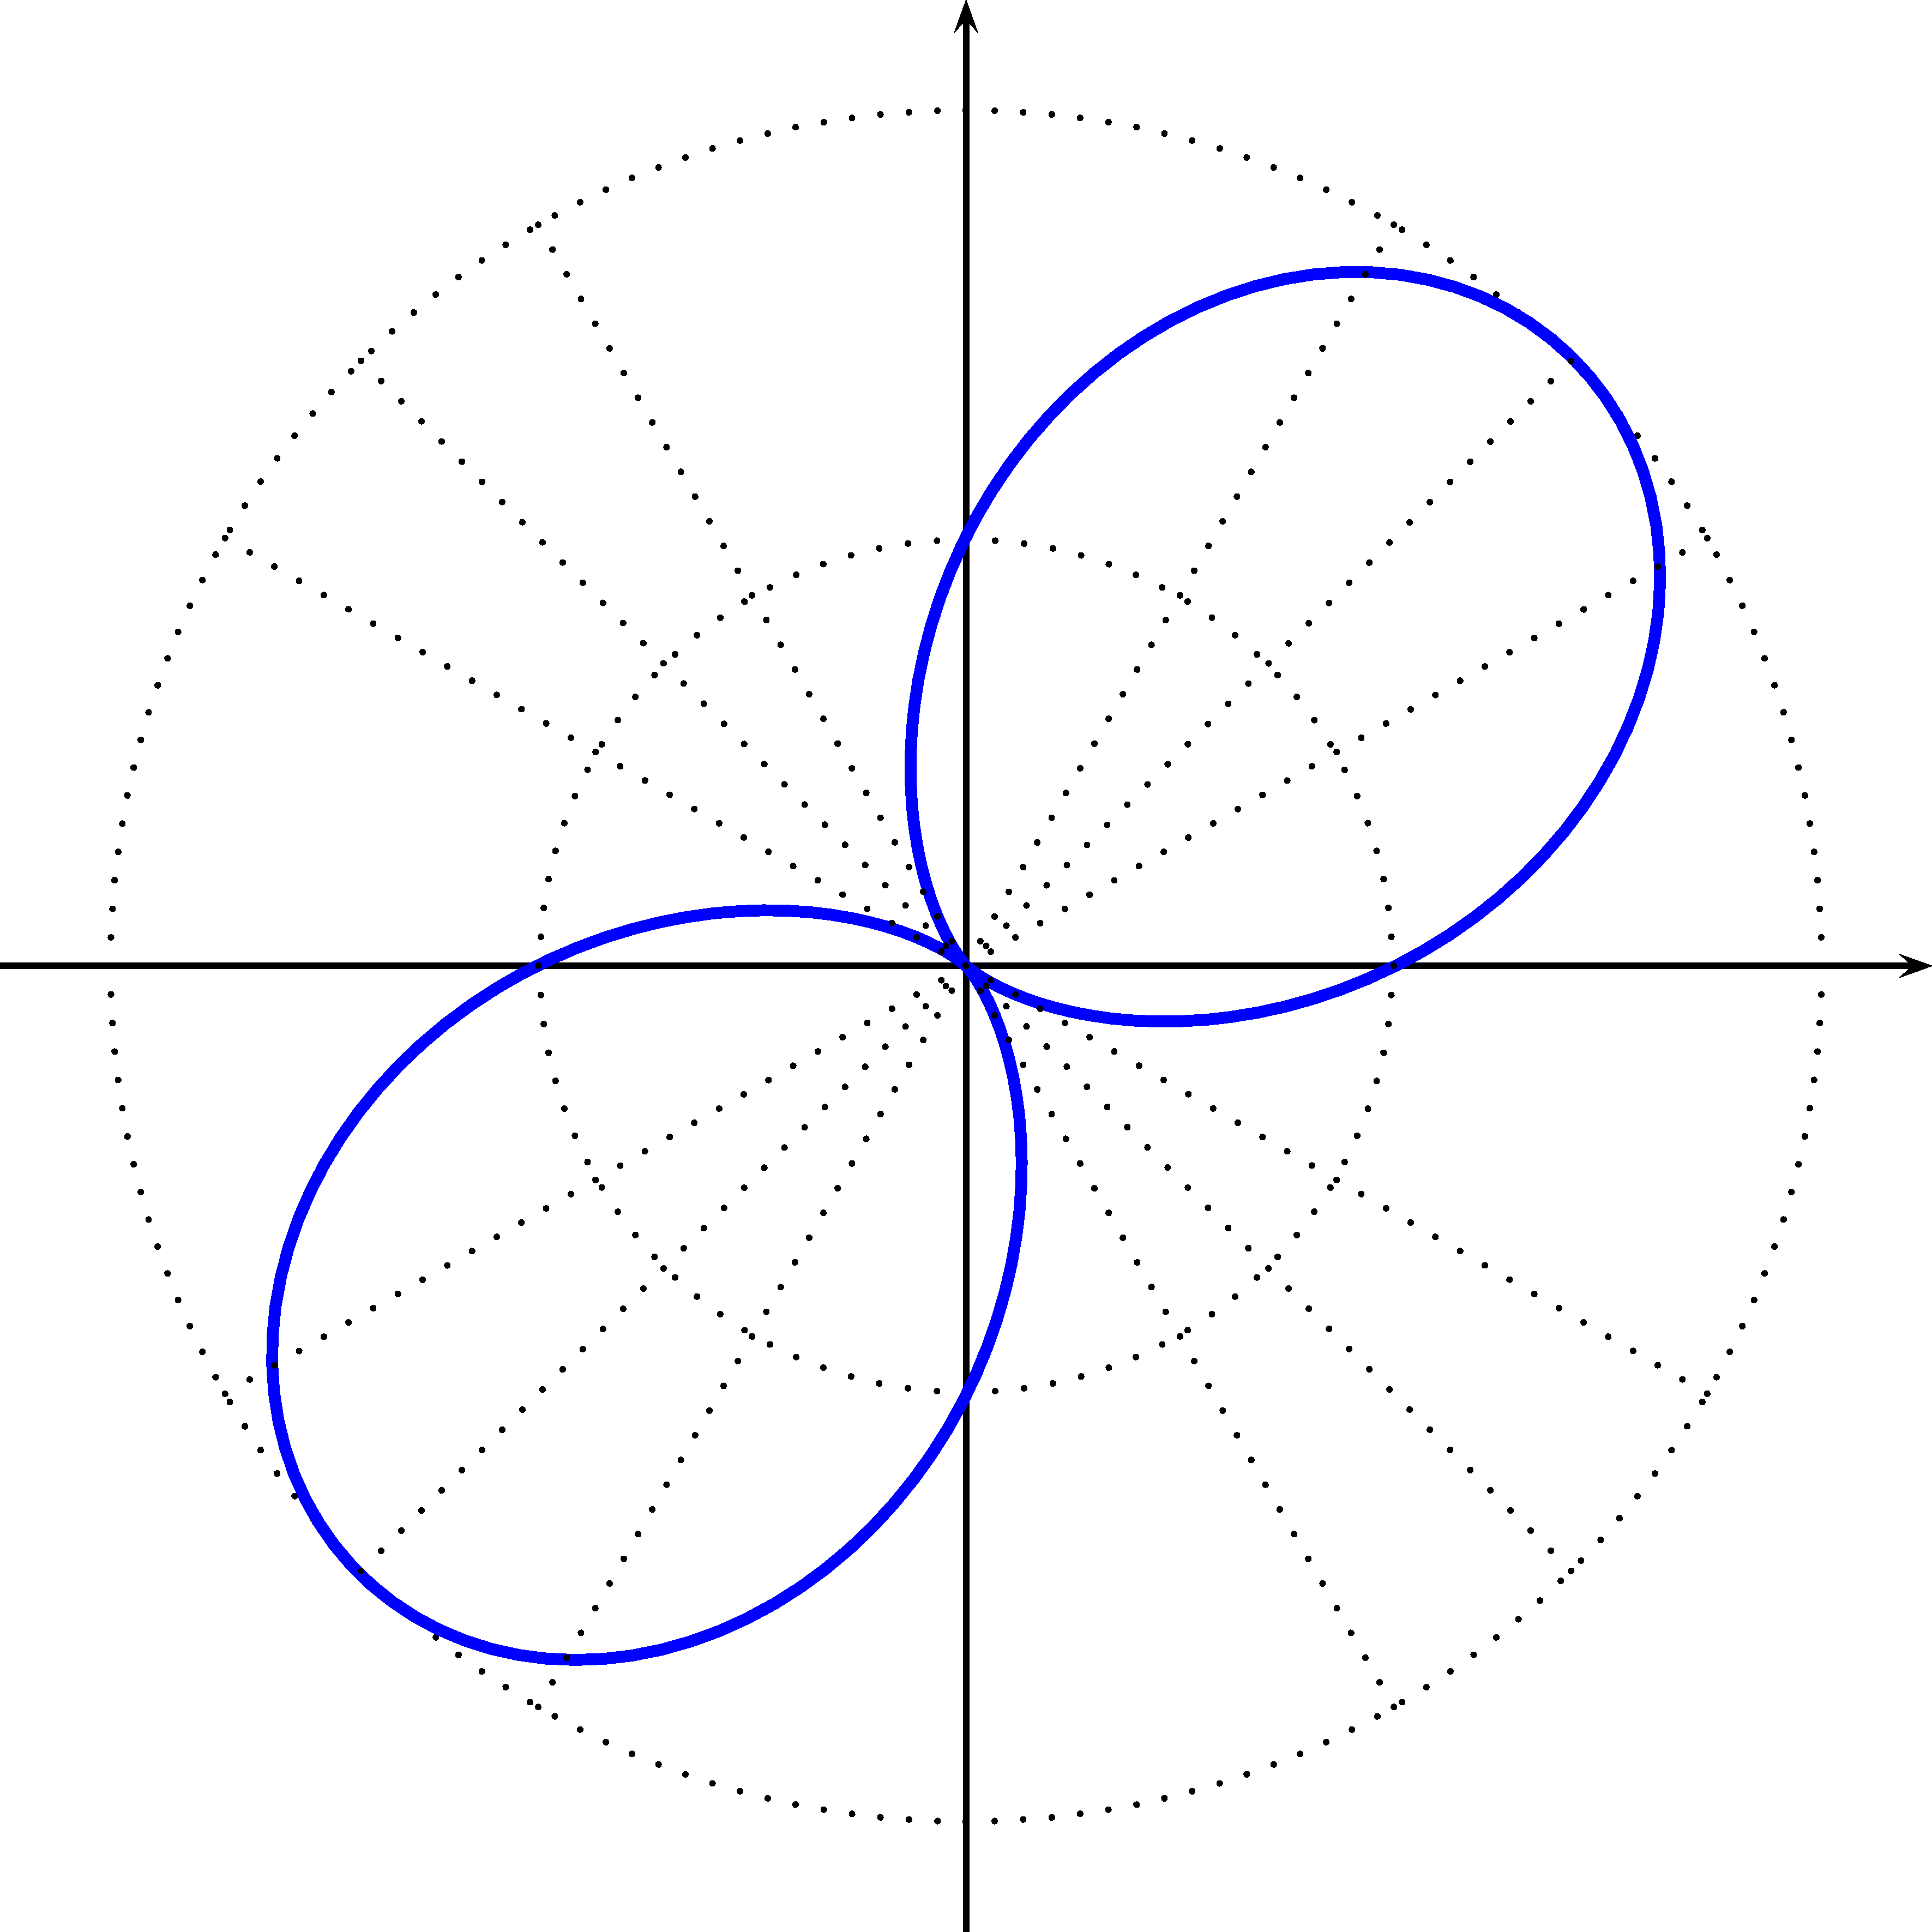
\includegraphics[width=0.5\linewidth]{resources/images/latex/ex1courbepolaire} \end{center}

\BeginKnitrBlock{example}
\protect\hypertarget{exm:unnamed-chunk-103}{}{\label{exm:unnamed-chunk-103}
}Dessinez \(r=1=\sin(\theta)\) pour \(\theta\in [0,2\pi]\).
\EndKnitrBlock{example}

\begin{center}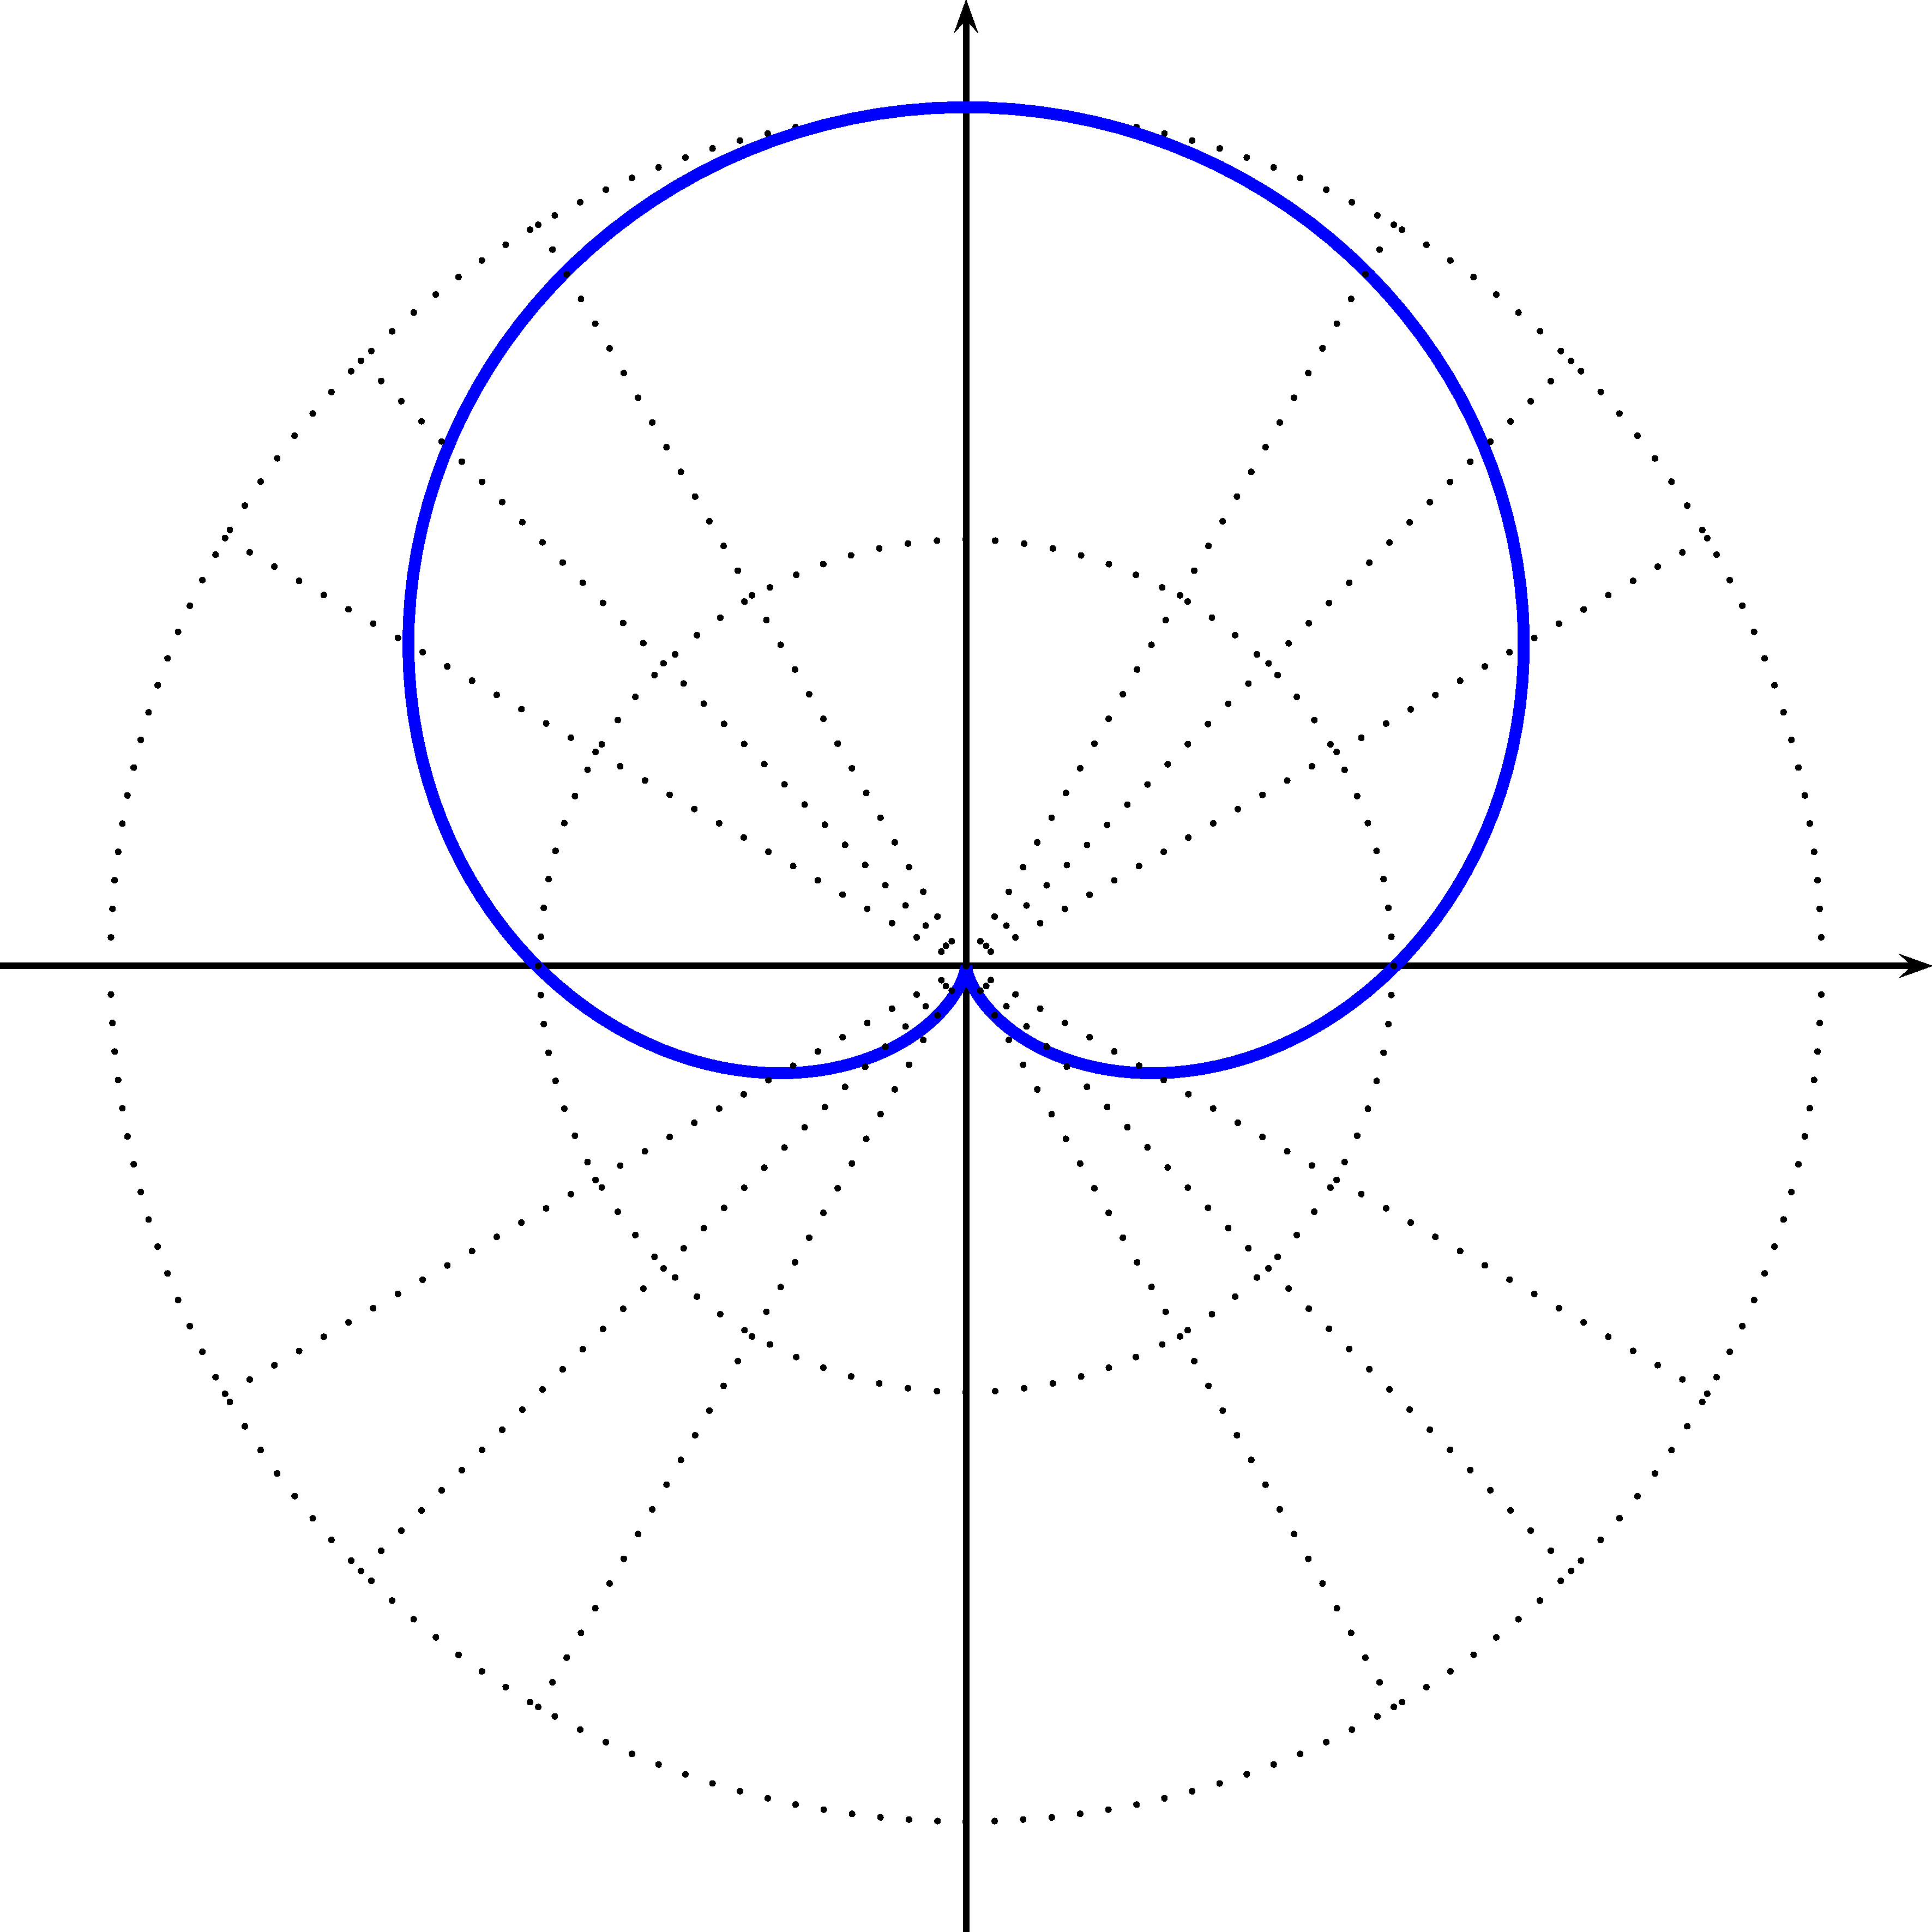
\includegraphics[width=0.5\linewidth]{resources/images/latex/ex2courbepolaire} \end{center}

\hypertarget{tangente-a-une-courbe-polaire}{%
\section{Tangente à une courbe
polaire}\label{tangente-a-une-courbe-polaire}}

Nous voulons maintenant déterminer les tangentes à des courbes polaires.
Nous savons que \(x=r\cos(\theta)\) et que \(y=r\sin(\theta)\). Si
\(r=f(\theta)\) alors nous avons que \(x=x(\theta)\) et \(y=y(\theta)\),
c'est-à-dire que \(x\) et \(y\) sont des fonctions de \(\theta\).

\BeginKnitrBlock{theorem}[Tangentes à une courbe polaire]
\protect\hypertarget{thm:tangente-polaire}{}{\label{thm:tangente-polaire}
\iffalse (Tangentes à une courbe polaire) \fi{} }Soit \(x\) et \(y\)
deux fonctions de \(\theta\). Si \(r=f(\theta)\), nous avons:
\begin{align*}
\dfrac{dy}{dx} &= \dfrac{f'(\theta)\sin(\theta)+f(\theta)\cos(\theta)}{f'(\theta)\cos(\theta)-f(\theta)\sin(\theta)}
\end{align*}
\EndKnitrBlock{theorem}

\BeginKnitrBlock{proof}
\iffalse{} {Preuve. } \fi{}Trouvons \(\dfrac{dx}{d\theta}\) et
\(\dfrac{dy}{d\theta}\). \begin{align*}
\dfrac{dx}{d\theta} &= \dfrac{d}{d\theta}\left[f(\theta)\cos(\theta)]\right] \\
&=  f'(\theta)\cos(\theta)-f(\theta)\sin(\theta) \\
\dfrac{dy}{d\theta} &= \dfrac{d}{d\theta}\left[f(\theta)\sin(\theta)]\right] \\
&=  f'(\theta)\sin(\theta)+f(\theta)\cos(\theta) 
\end{align*} Ainsi, \begin{align*}
\dfrac{dy}{dx} &= \dfrac{\dfrac{dy}{d\theta}}{\dfrac{dx}{d\theta}} \\
&= \dfrac{f'(\theta)\sin(\theta)+f(\theta)\cos(\theta)}{f'(\theta)\cos(\theta)-f(\theta)\sin(\theta)}
\end{align*}
\EndKnitrBlock{proof}

Nous avons maintenant une formule pour déterminer la pente de la droite
tangente.

\BeginKnitrBlock{example}
\protect\hypertarget{exm:unnamed-chunk-105}{}{\label{exm:unnamed-chunk-105}
}Trouvez l'équation de la droite tangente en \(\theta=\frac{\pi}{2}\) de
\(r=1+\sin(2\theta)\).
\EndKnitrBlock{example}
\vspace*{8cm}

\BeginKnitrBlock{example}
\protect\hypertarget{exm:unnamed-chunk-106}{}{\label{exm:unnamed-chunk-106}
}Soit l'équation \(r=2\cos(\theta)\).

\begin{enumerate}
\def\labelenumi{\alph{enumi}.}
\tightlist
\item
  Trouvez la dérivée \(\dfrac{dy}{dx}\).
\item
  Évaluez \(\left.\dfrac{dy}{dx}\right|_{\theta=\frac{\pi}{4}}\).
\item
  Évaluez \(\left.\dfrac{dy}{dx}\right|_{\theta=\frac{\pi}{3}}\).
\end{enumerate}
\EndKnitrBlock{example}
\vspace*{10cm}

\BeginKnitrBlock{example}
\protect\hypertarget{exm:unnamed-chunk-107}{}{\label{exm:unnamed-chunk-107}
}Trouvez la dérivée de la rose de Ghandi,
\(r=\cos\left(\dfrac{3\theta}{2}\right)\).
\EndKnitrBlock{example}
\vspace*{6cm}

\hypertarget{aire-dune-region}{%
\section{Aire d'une région}\label{aire-dune-region}}

Nous voulons maintenant trouver une formule afin de calculer l'aire
d'une région formée par une courbe définie par \(r=f(\theta)\) avec
\(\theta_a\leq \theta \leq \theta_b\).

Rappelons que l'aire \(A\) d'un secteur de cercle de rayon \(r\) est
donnée par \(A=\dfrac{1}{2}r^2\theta\).

La figure \ref{fig:airepolaire1} représente la surface que nous désirons
trouver.

\begin{figure}

{\centering 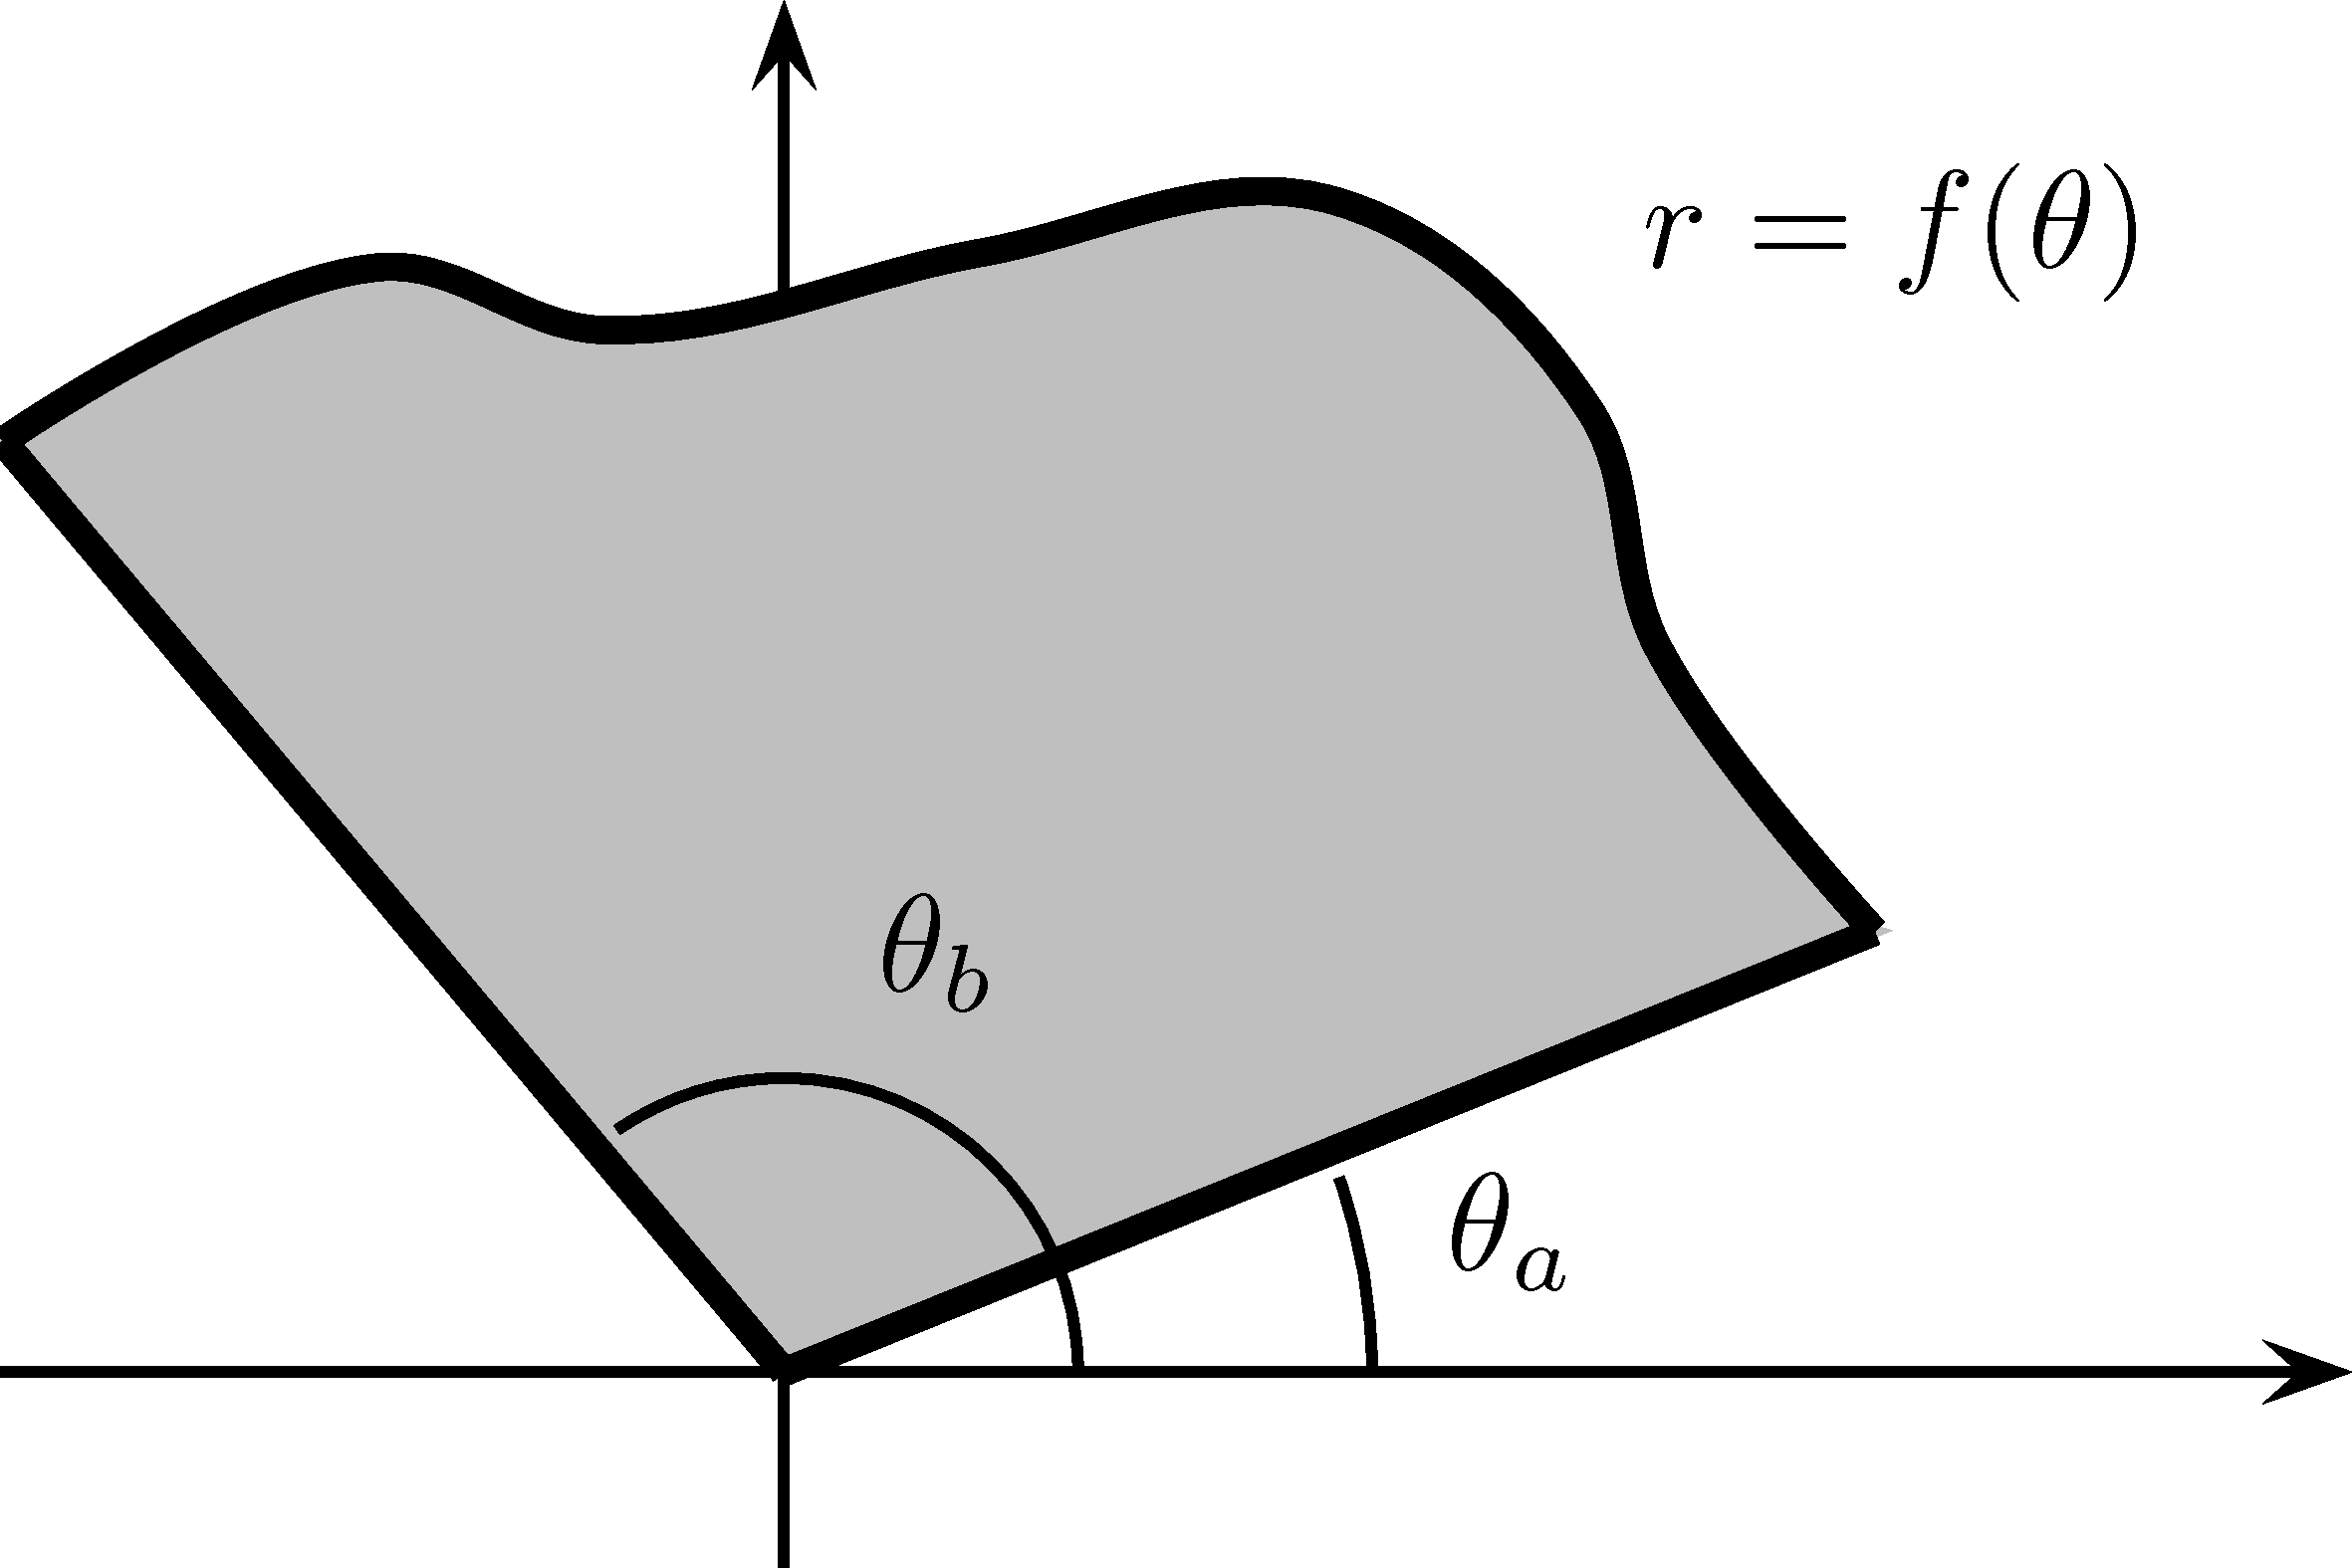
\includegraphics[width=0.5\linewidth]{resources/images/latex/airepolaire1} 

}

\caption{Aire d'une courbe polaire}\label{fig:airepolaire1}
\end{figure}

Divisons l'intervalle \(\theta_a\leq \theta \leq \theta_b\) en \(N\)
partitions de longueur \(\Delta \theta_i=\theta_i-\theta_{i-1}\) pour
\(i=1,\ldots,N\). L'ensemble \begin{align*}
\{\theta_0=\theta_a,\theta_1,...,\theta_{N-1},\theta_{N}=\theta_b\}
\end{align*} est appelée partition de
\(\theta_a\leq \theta \leq \theta_b\). L'aire de chacun de ces secteurs
peut être approchée par: \begin{align*}
A_i\approx \dfrac{1}{2}[f(\theta_i^*)]^2\Delta \theta_i, \quad \text{où $\theta_i^*\in [\theta_{i-1},\theta_{i}]$}
\end{align*}

La figure \ref{fig:airepolaire2} représente une partition.

\begin{figure}

{\centering 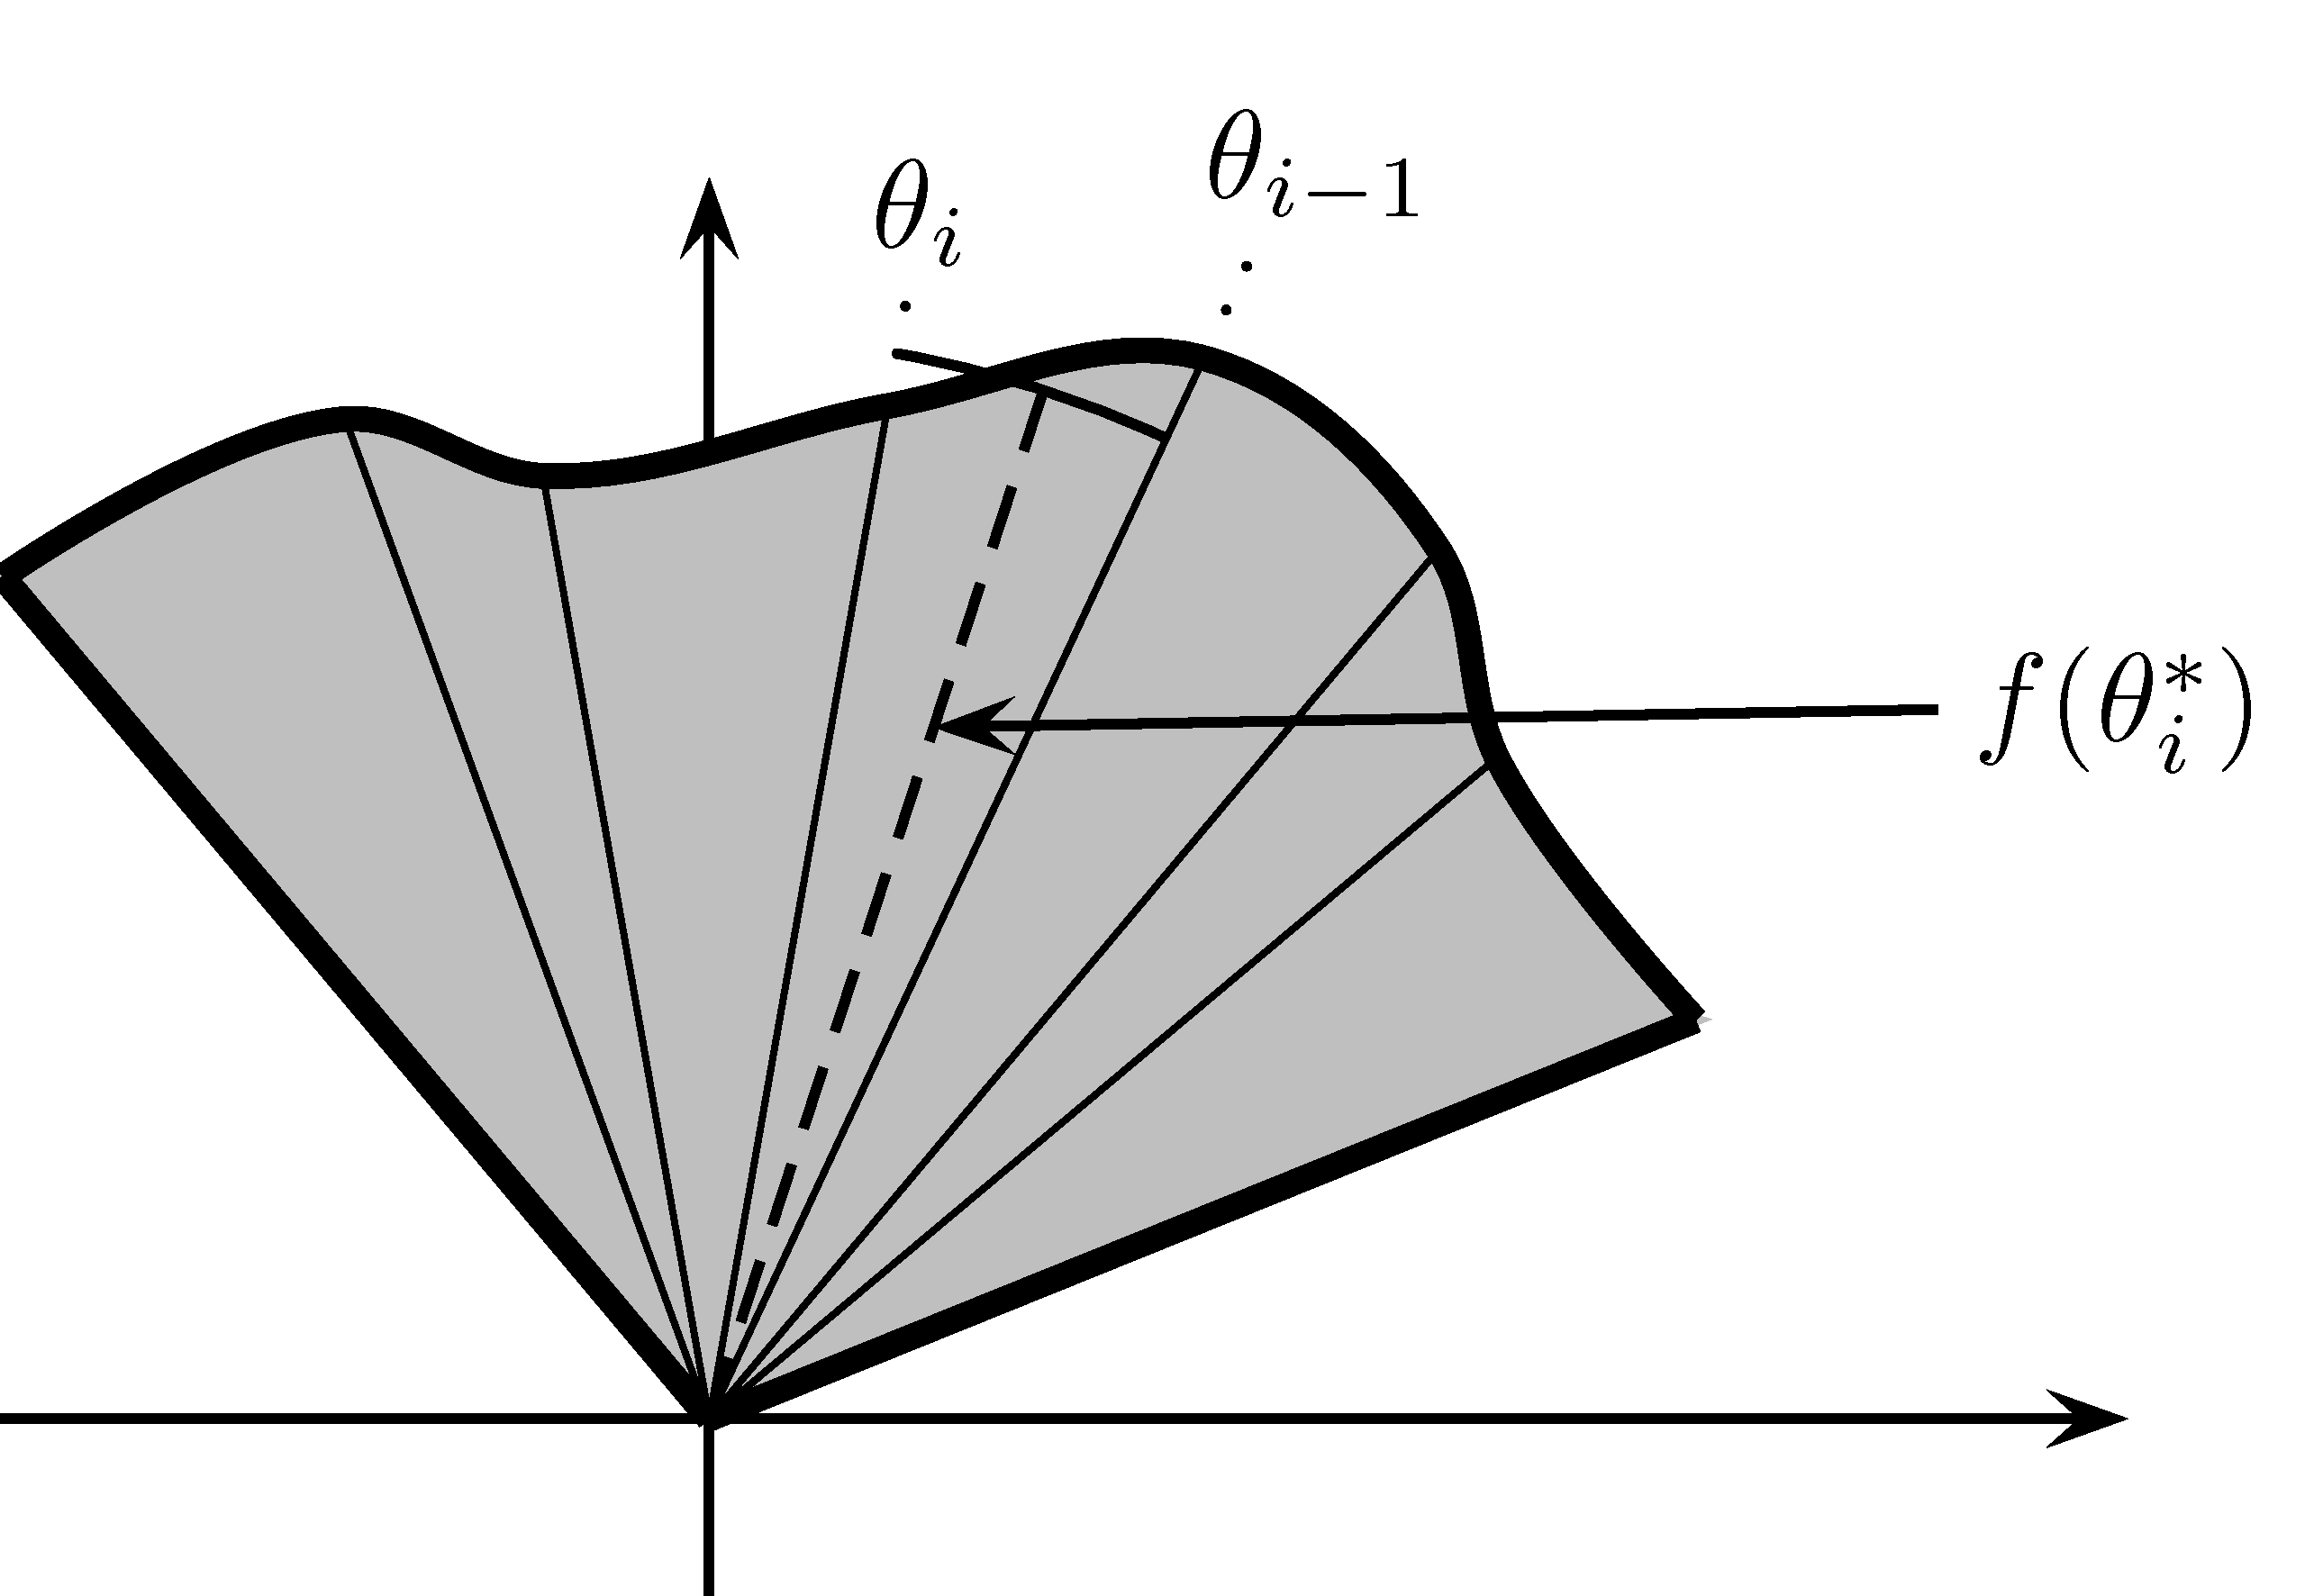
\includegraphics[width=0.5\linewidth]{resources/images/latex/airepolaire2} 

}

\caption{Aire d'une courbe polaire: séparation en secteurs}\label{fig:airepolaire2}
\end{figure}

Nous voulons trouver l'aire totale, c'est-à-dire la somme des surfaces
des \(N\) secteurs: \begin{align*}
A\approx \sum_{i=1}^N\dfrac{1}{2}[f(\theta_i^*)]^2\Delta \theta_i
\end{align*} Nous remarquons que cette somme est une somme de Riemann.
Ainsi, en prenant la limite lorsque \(N\) tend vers l'infini, nous
obtenons: \begin{align*}
A=\lim_{N\rightarrow \infty } \sum_{i=1}^N\dfrac{1}{2}[f(\theta_i^*)]^2\Delta \theta_i=\int_{\theta_a}^{\theta_b}\dfrac{1}{2}[f(\theta)]^2d \theta
\end{align*}

D'où, l'aire est donnée par: \begin{align*}
A &= \int_{\theta_a}^{\theta_b}\dfrac{1}{2}[f(\theta)]^2 d\theta
\end{align*}

\BeginKnitrBlock{example}
\protect\hypertarget{exm:unnamed-chunk-108}{}{\label{exm:unnamed-chunk-108}
}Calculez l'aire de la région formée par \(r=1+\sin(2\theta)\).
\EndKnitrBlock{example}

\begin{center}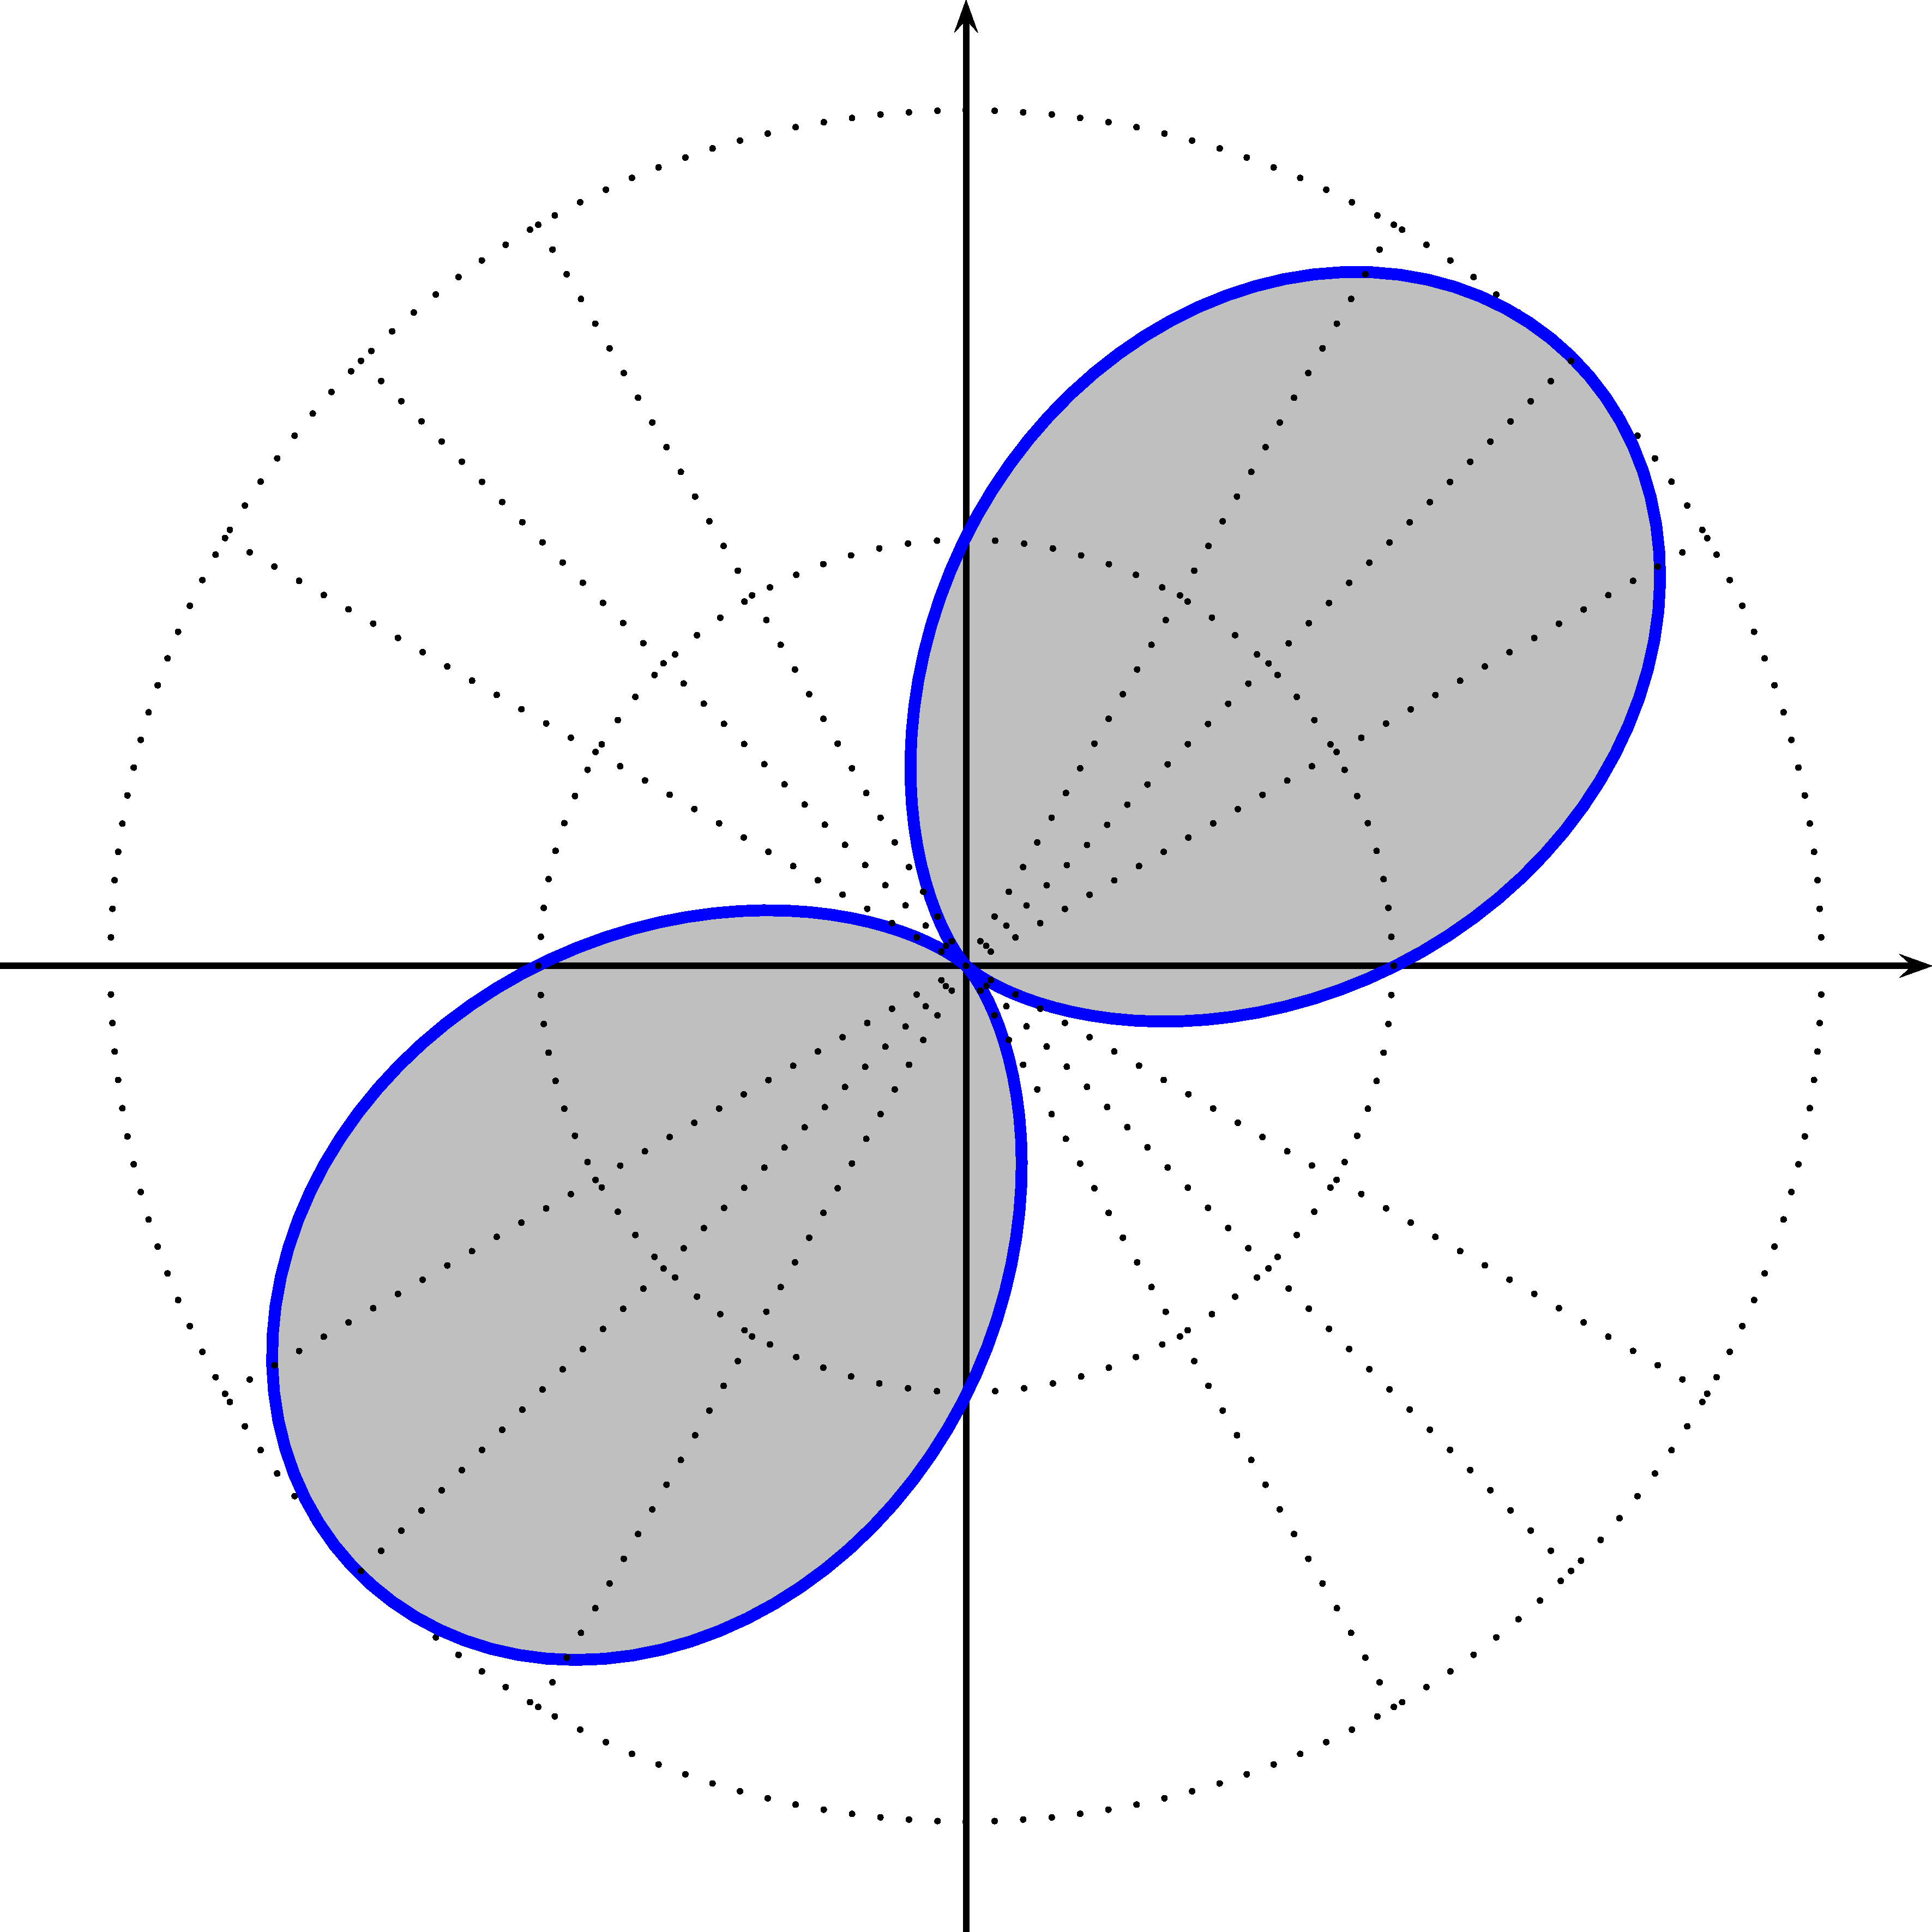
\includegraphics[width=0.5\linewidth]{resources/images/latex/ex1airepolaire} \end{center}
\vspace*{10cm}

\BeginKnitrBlock{example}
\protect\hypertarget{exm:unnamed-chunk-109}{}{\label{exm:unnamed-chunk-109}
}Calculez l'aire située au-dessus du cercle \(r=3\sin(\theta)\) et en
dessous de la cardioïde \(r=1+\sin(\theta)\).
\EndKnitrBlock{example}

\begin{center}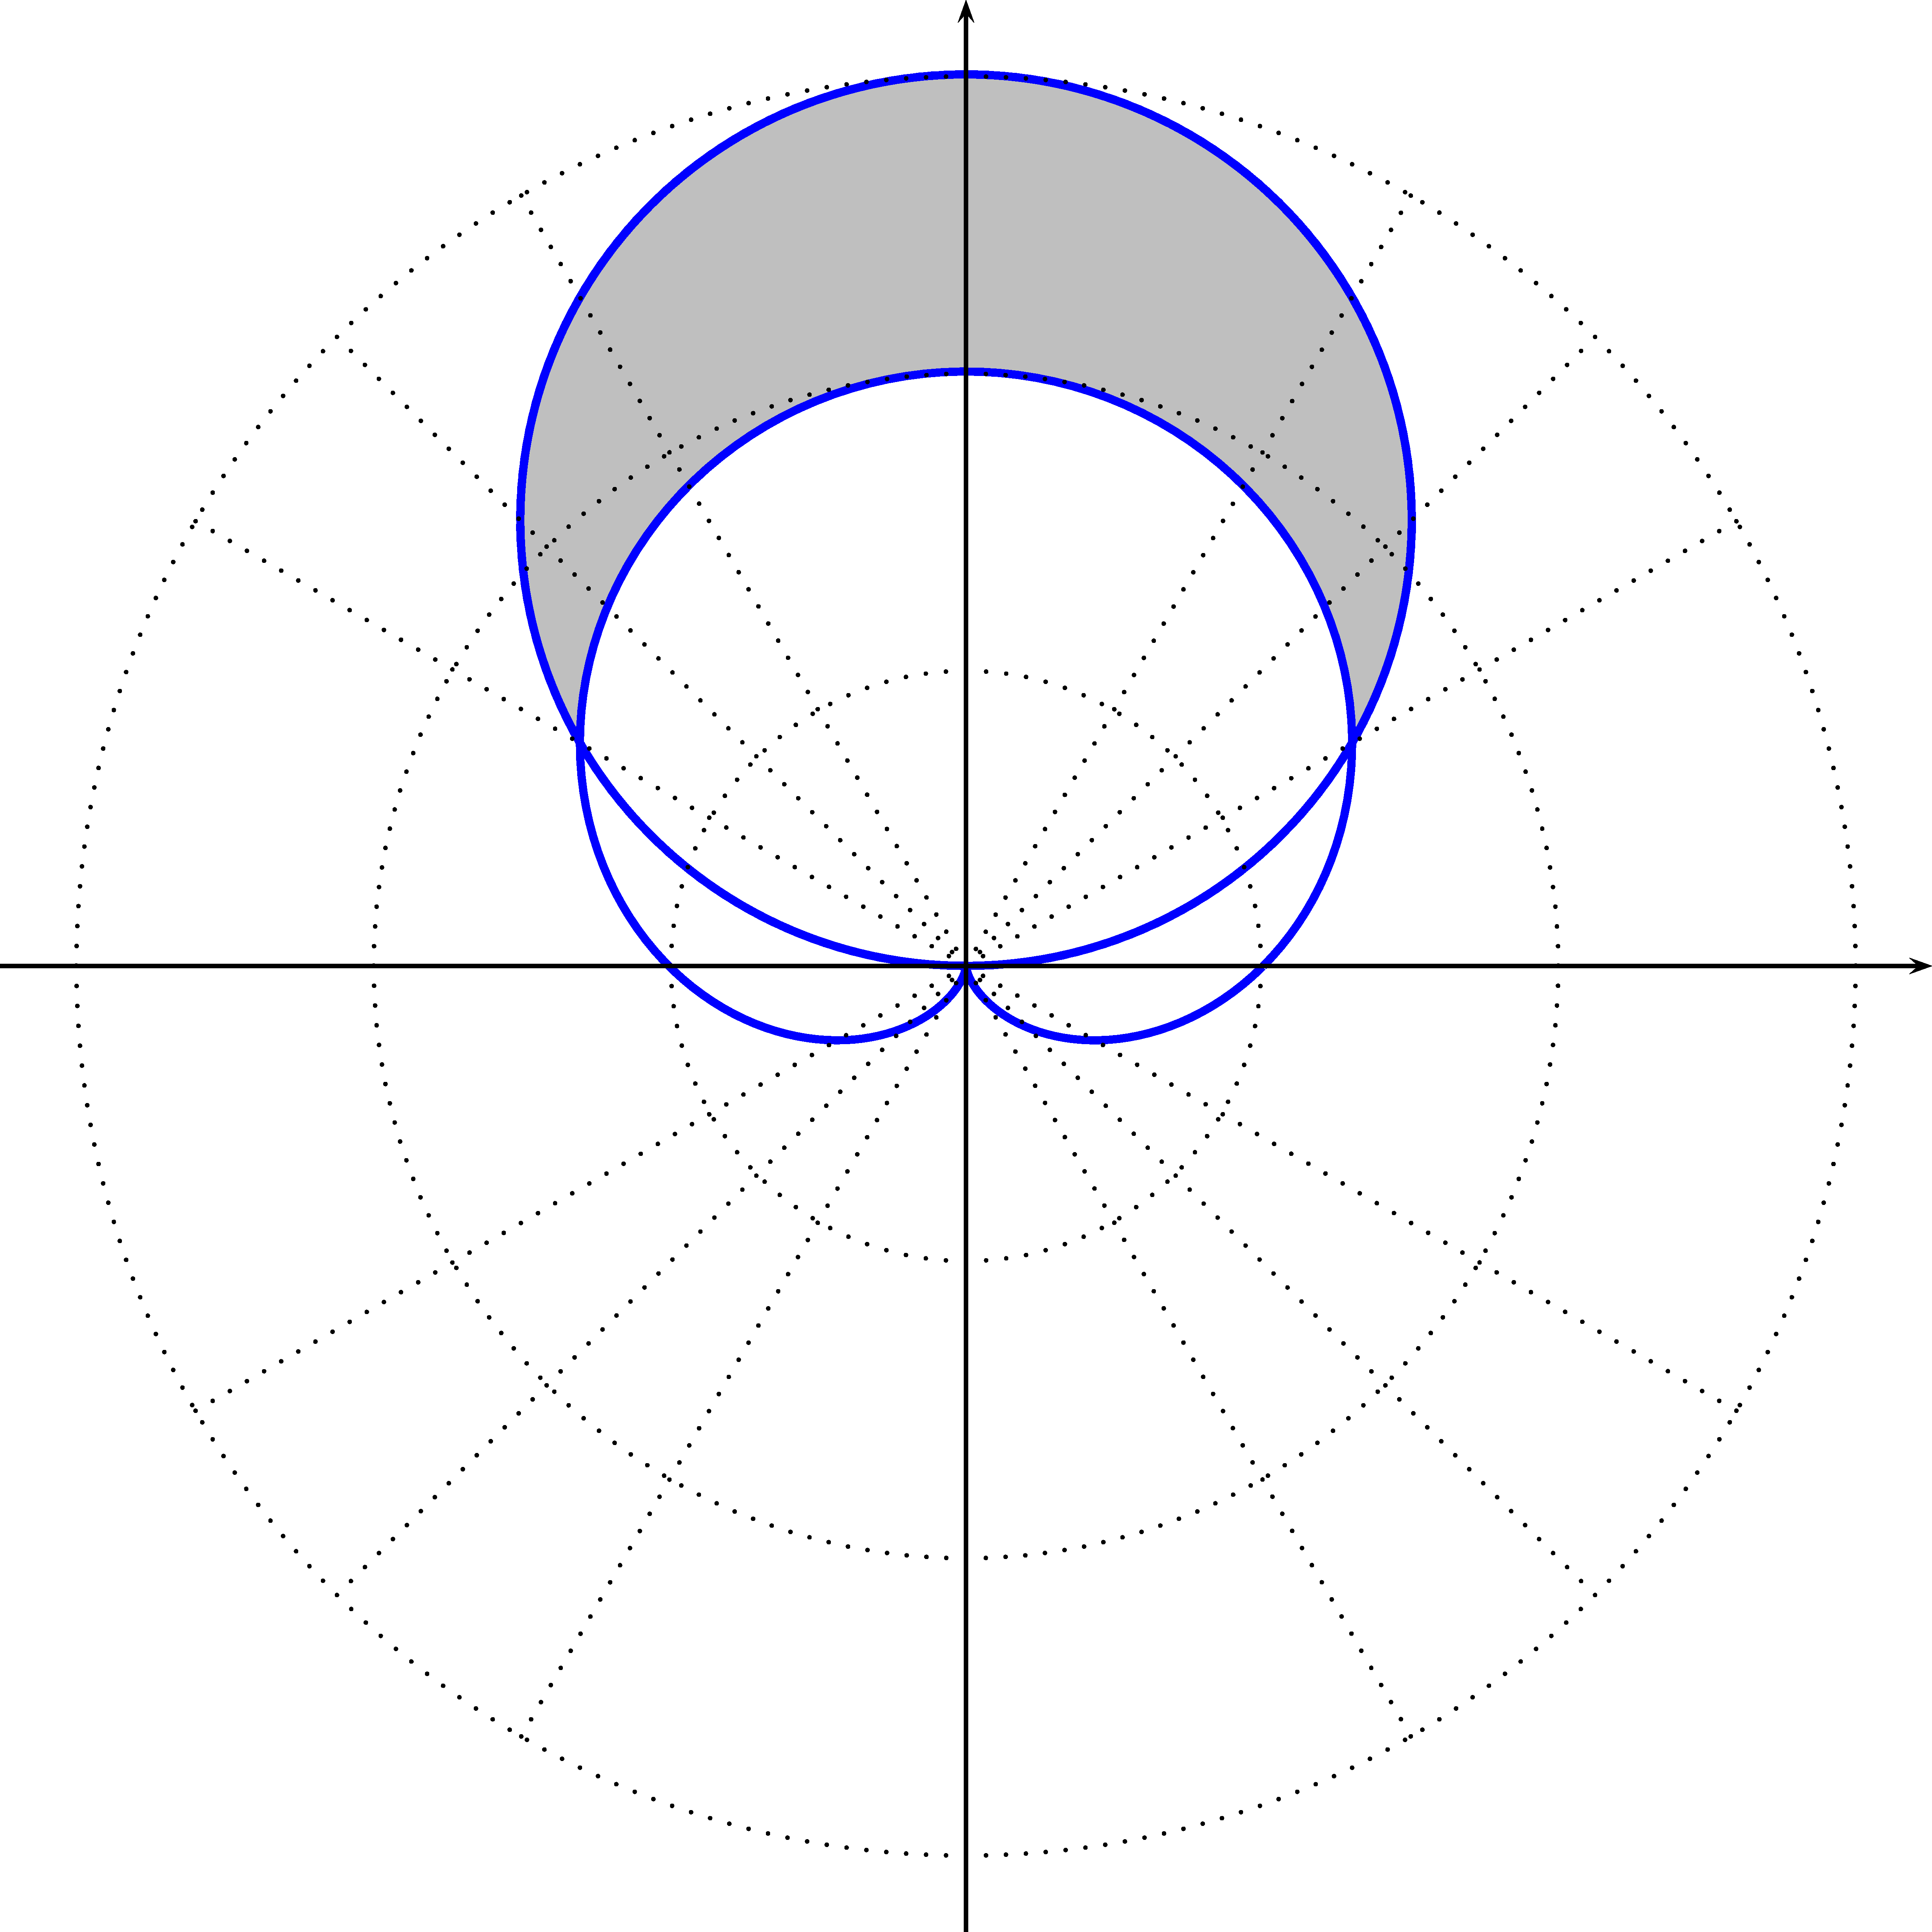
\includegraphics[width=0.5\linewidth]{resources/images/latex/ex2airepolaire} \end{center}
\vspace*{10cm}

\BeginKnitrBlock{example}
\protect\hypertarget{exm:unnamed-chunk-110}{}{\label{exm:unnamed-chunk-110}
}Calculez l'aire d'une seule feuille de \(r=1+\sin(\theta)\) avec
\(0\leq \theta \leq \frac{\pi}{3}\).
\EndKnitrBlock{example}
\vspace*{10cm}

\BeginKnitrBlock{example}
\protect\hypertarget{exm:unnamed-chunk-111}{}{\label{exm:unnamed-chunk-111}
}Calculez l'aire du quadrifolium \(r=\cos(2\theta)\) si un seul pétale
se trouve dans l'intervalle
\(\frac{\pi}{4}\leq \theta \leq \frac{3\pi}{4}\).
\EndKnitrBlock{example}
\vspace*{10cm}

\hypertarget{longueur-dune-courbe}{%
\section{Longueur d'une courbe}\label{longueur-dune-courbe}}

\BeginKnitrBlock{theorem}[Longueur d'une courbe en coordonnées polaires]
\protect\hypertarget{thm:unnamed-chunk-112}{}{\label{thm:unnamed-chunk-112}
\iffalse (Longueur d'une courbe en coordonnées polaires) \fi{} }La
longueur d'une courbe en coordonnées polaires définie par
\(r=f(\theta)\) où \(\theta_a\leq\theta\leq\theta_b\) est donnée par:
\begin{align*}
L=\int_{\theta_a}^{\theta_b}\sqrt{\left(\dfrac{dr}{d\theta}\right)^2+r^2}d\theta
\end{align*}
\EndKnitrBlock{theorem}

\BeginKnitrBlock{proof}
\iffalse{} {Preuve. } \fi{}La démonstration suivante escamote plusieurs
utilisations des sommes de Riemann pour simplifier.

Nous savons que: \begin{align*}
L &= \int_a^b \sqrt{1+\left(\dfrac{dy}{dx}\right)^2}dx \\
&= \int_a^b \sqrt{(dx)^2\left(1+\left(\dfrac{dy}{dx}\right)^2\right)} \\
&= \int_a^b \sqrt{(dx)^2+(dy)^2} \\
&= \int_a^b \sqrt{\left(\dfrac{dx}{d\theta}d\theta\right)^2+\left(\dfrac{dy}{d\theta}d\theta\right)^2} \\
&= \int_a^b \sqrt{\left(\dfrac{dx}{d\theta}\right)^2+\left(\dfrac{dy}{d\theta}\right)^2}d\theta
\end{align*} Nous savons par le théorème \ref{thm:tangente-polaire} ce
que sont \(\dfrac{dx}{d\theta}\) et \(\dfrac{dy}{d\theta}\). Ainsi:
\begin{align*}
L &= \int_a^b \sqrt{\left(\dfrac{dr}{d\theta}\cos(\theta)-r\sin(\theta)\right)^2+\left(\dfrac{dr}{d\theta}\sin(\theta)+r\cos(\theta)\right)^2}d\theta \\
&= \ldots \\
&= \int_{\theta_a}^{\theta_b}\sqrt{\left(\dfrac{dr}{d\theta}\right)^2+r^2}d\theta 
\end{align*}
\EndKnitrBlock{proof}

Voici quelques exemple de longueurs d'arc.

\BeginKnitrBlock{example}
\protect\hypertarget{exm:unnamed-chunk-114}{}{\label{exm:unnamed-chunk-114}
}Calculez la longueur d'arc de \(r=e^{2\theta}\) avec
\(\theta\in[0,2\pi]\).
\EndKnitrBlock{example}
\vspace*{8cm}

\BeginKnitrBlock{example}
\protect\hypertarget{exm:unnamed-chunk-115}{}{\label{exm:unnamed-chunk-115}
}Calculez la longueur d'arc de \(r=2-2\cos(\theta)\) avec
\(\theta\in[0,2\pi]\).
\EndKnitrBlock{example}
\vspace*{8cm}

\BeginKnitrBlock{example}
\protect\hypertarget{exm:unnamed-chunk-116}{}{\label{exm:unnamed-chunk-116}
}Calculez la longueur d'arc de \(r=ae^{-b\theta}\) avec
\(\theta\in[0,\infty[\) et \(b>0\).
\EndKnitrBlock{example}
\vspace*{10cm}

\BeginKnitrBlock{example}
\protect\hypertarget{exm:unnamed-chunk-117}{}{\label{exm:unnamed-chunk-117}
}Calculez la longueur d'arc de \(r=a(1-\sin(\theta))\) avec
\(\theta\in[0,2\pi]\).
\EndKnitrBlock{example}
\vspace*{8cm}

\hypertarget{geogebra-polaire}{%
\section{GeoGebra}\label{geogebra-polaire}}

\hypertarget{applet_container}{}

\newpage

\hypertarget{pages-supplementaires-2}{%
\section{Pages supplémentaires}\label{pages-supplementaires-2}}

Des pages blanches supplémentaires pour ajouter, potentiellement, de
nouveaux exemples et exercices.

\multido{\i=1+1}{4}{
\newpage
\mbox{}
}

\hypertarget{fctvar}{%
\chapter{Les fonctions de plusieurs variables}\label{fctvar}}

Vous trouverez à la section \ref{geogebra-fctvar} une application
\href{https://www.geogebra.org/?lang=fr}{GeoGebra} vous permettant de
visualiser des coupes transversales et des courbes de niveaux. À noter
que cette application n'est disponible que dans la version en ligne de
ce document.

\hypertarget{introduction-3}{%
\section{Introduction}\label{introduction-3}}

Jusqu'à présent dans vos cours de calcul différentiel et intégral, nous
n'avons étudié que les fonctions d'une seule variable, c'est-à-dire des
fonctions de la forme \(y=f(x)\). Nous avons appris à dessiner ces
fonctions, à les dériver, à les intégrer, etc. Par contre, il est utile
d'étudier les fonctions de plus d'une variable car la plupart des
phénomènes étudiés dépendent de plus d'un paramètre.

Dans ce chapitre, nous reprendrons les différents thèmes étudiés sur les
fonctions d'une seule variable, pour les généraliser sur les fonctions
de plusieurs variables.

\hypertarget{definitions}{%
\section{Définitions}\label{definitions}}

Débutons en rappelant le concept de fonction et en le généralisant aux
fonctions de deux variables ou plus.

\BeginKnitrBlock{definition}[Fonction]
\protect\hypertarget{def:unnamed-chunk-119}{}{\label{def:unnamed-chunk-119}
\iffalse (Fonction) \fi{} }Soit un ensemble \(A\) et un ensemble \(B\).
Une fonction \(f\) est une application qui pour chaque élément
\(x\in A\) lui associe un seul élément \(y\in B\). On note cette
fonction \begin{align*}
f:\ A&\longrightarrow  B\\
x&\longrightarrow  y=f(x)
\end{align*}

\begin{itemize}
\tightlist
\item
  L'ensemble \(A\) se nomme \textbf{domaine} de \(f\), noté
  \(\text{dom}(f)\).
\item
  L'ensemble \(B\) est le \textbf{codomaine} de la fonction \(f\), noté
  \(\text{codom}(f)\).
\end{itemize}
\EndKnitrBlock{definition}

\BeginKnitrBlock{definition}[Image d'une fonction]
\protect\hypertarget{def:unnamed-chunk-120}{}{\label{def:unnamed-chunk-120}
\iffalse (Image d'une fonction) \fi{} }L'image d'une fonction est
l'ensemble de tous les éléments du codomaine qui sont obtenus par la
fonction \(f\). Nous notons l'image \(\text{ima}(f)\). En langage
mathématique, l'image s'écrit comme suit: \begin{align*}
\text{ima}(f):=\{y|y=f(x),\forall x\in dom(f)\}
\end{align*} Il est à remarquer que
\(\text{ima}(f)\subseteq \text{codom}(f)\).
\EndKnitrBlock{definition}

La distinction entre l'image et le codomaine est représentée à la figure
\ref{fig:representationfonction}. Le codomaine est l'ensemble \(B\)
tandis que l'image est l'ensemble de tous les éléments de \(B\) qui sont
reliés à un ou plusieurs éléments de \(A\) par la fonction (ici l'image
est la région ombragée).

\begin{figure}

{\centering 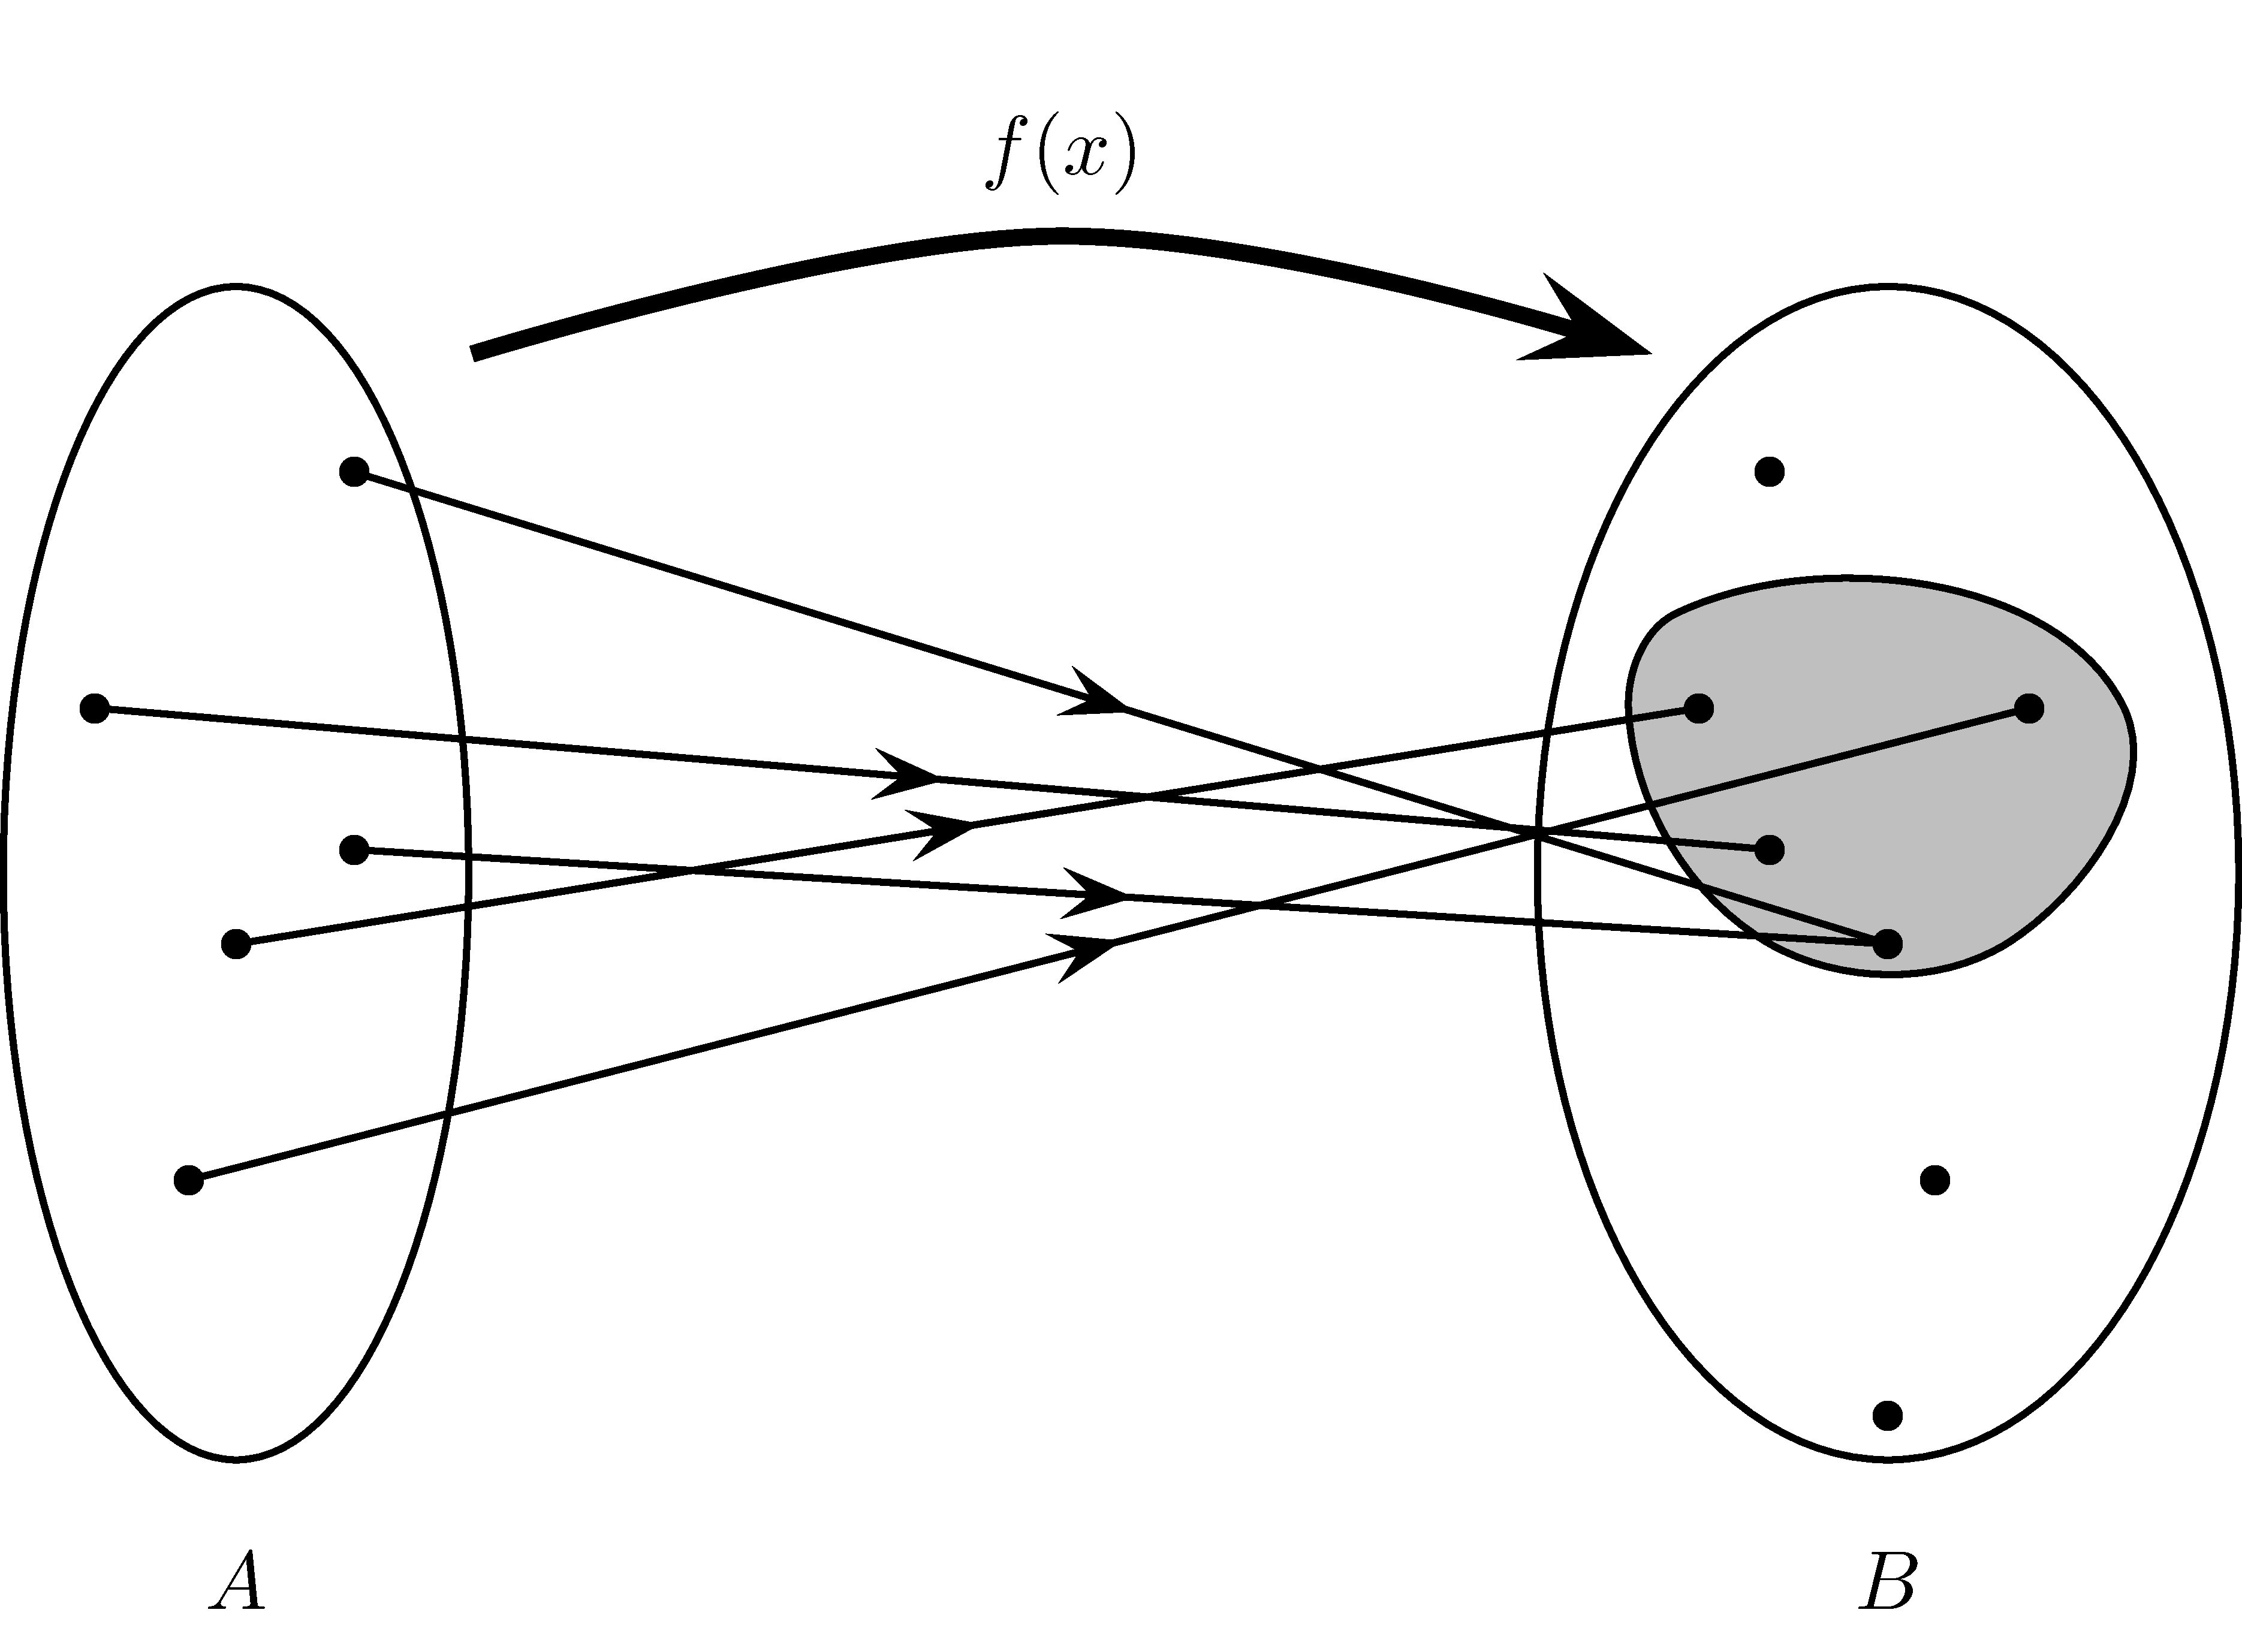
\includegraphics[width=0.5\linewidth]{resources/images/latex/representationfonction} 

}

\caption{Graphique saggital représentant une fonction.}\label{fig:representationfonction}
\end{figure}

Jusqu'à maintenant, nous avons étudié les fonctions ayant comme domaine
un sous-ensemble de la droite des réels. Dans ce cours, nous étudierons
des fonctions ayant comme domaine un sous-ensemble \(\mathbb{R}^n\), où
\(n\in\mathbb{N}\). En langage mathématique, ces fonctions s'écrivent:
\begin{align*}
f: D\subseteq \mathbb{R}^n &\longrightarrow \mathbb{R}\\
(x_1,..,x_n)&\longrightarrow z=f(x_1,..,x_n)
\end{align*} où \(x_1\), \ldots{}, \(x_n\) sont \(n\) variables
indépendantes.

\hypertarget{graphiques-divers}{%
\section{Graphique}\label{graphiques-divers}}

Lorsque nous avons une fonction \(y=f(x)\), son graphe correspond à une
courbe dans le plan cartésien, c'est-à-dire dans \(\mathbb{R}^2\). Pour
parvenir à dessiner cette courbe, on fait correspondre une valeur de
\(y\) pour chaque valeur de \(x\).

Lorsque nous somme en présence d'une fonction de deux variables
\(z=f(x,y)\), le graphique de cette fonction est une surface dans
l'espace de trois dimensions, \(\mathbb{R}^3\).

Par contre, lorsque notre fonction possède plus de deux variables, il
devient difficile, voire impossible de la représenter graphiquement. Il
faudrait utiliser des espaces de plus de trois dimensions.

\BeginKnitrBlock{remark}
\iffalse{} {Remarque. } \fi{}Dans le cadre de ce cours, nous nous en
tiendrons à des fonctions de une, deux ou trois variables.
\EndKnitrBlock{remark}

La figure \ref{fig:point3d} montre de quelle façon nous pouvons
représenter le point (a,b,f(a,b)) dans l'espace à trois dimensions.

\begin{figure}

{\centering 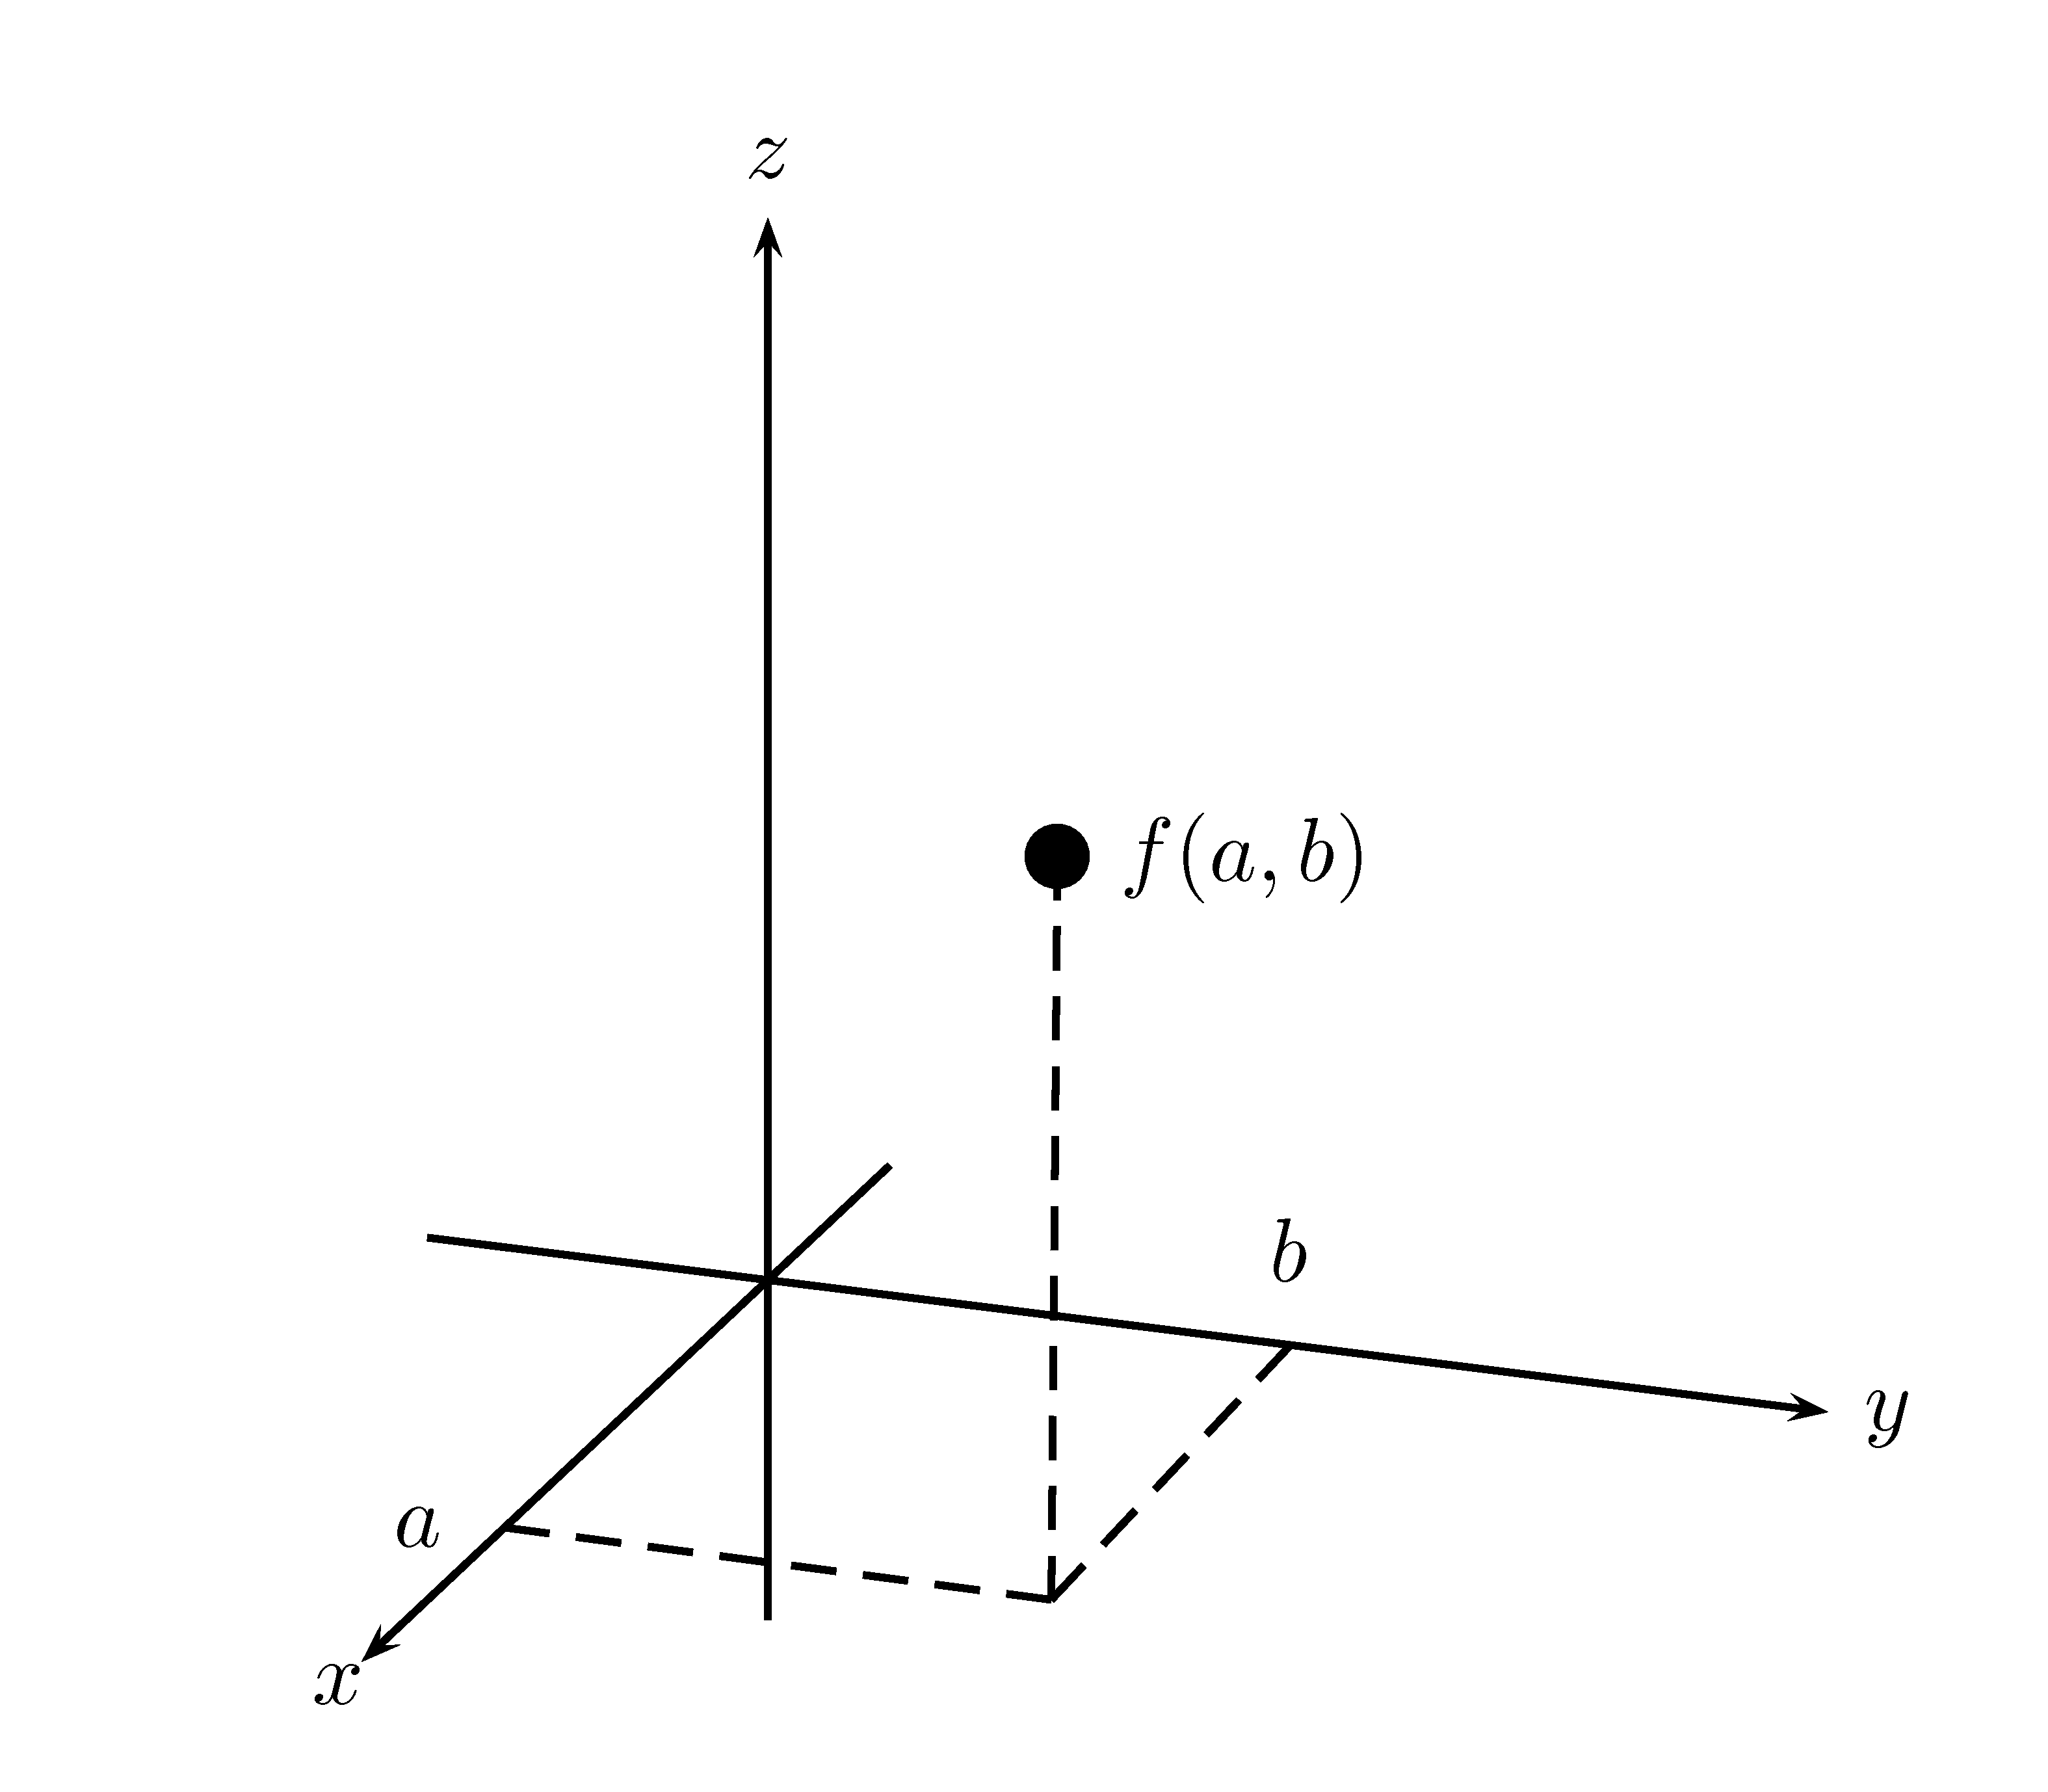
\includegraphics[width=0.75\linewidth]{resources/images/latex/point3d} 

}

\caption{Représentation en trois dimensions d'un point.}\label{fig:point3d}
\end{figure}

Nous allons maintenant présenter plusieurs fonctions accompagnées de
leur graphique.

Les figures suivantes représentent des fonctions usuelles que nous
rencontrerons régulièrement dans le cours.

\begin{figure}

{\centering 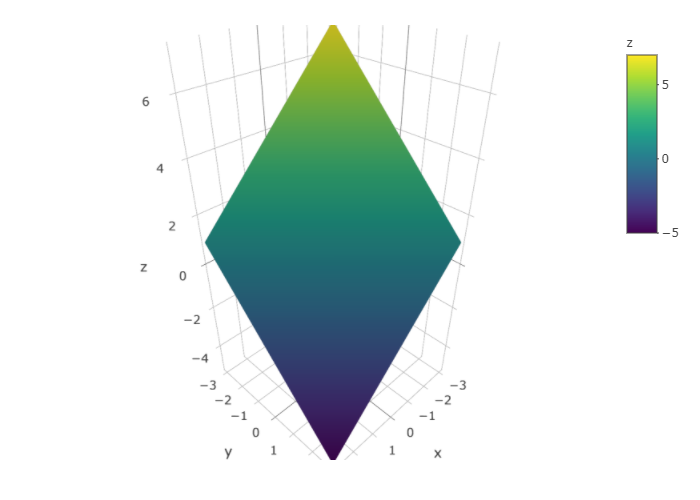
\includegraphics[width=0.8\linewidth]{resources/images/plan} 

}

\caption{Plan: $z=1-x-y$}\label{fig:plan}
\end{figure}

\begin{figure}

{\centering 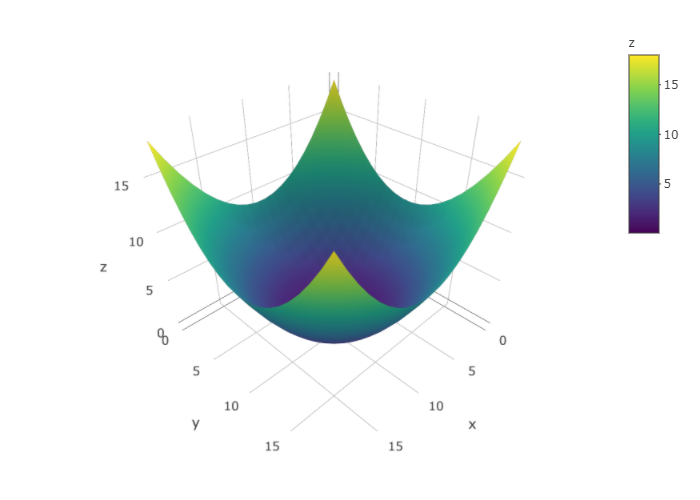
\includegraphics[width=0.8\linewidth]{resources/images/paraboloide} 

}

\caption{Paraboloïde: $z=x^2+y^2$}\label{fig:paraboloide}
\end{figure}

\begin{figure}

{\centering 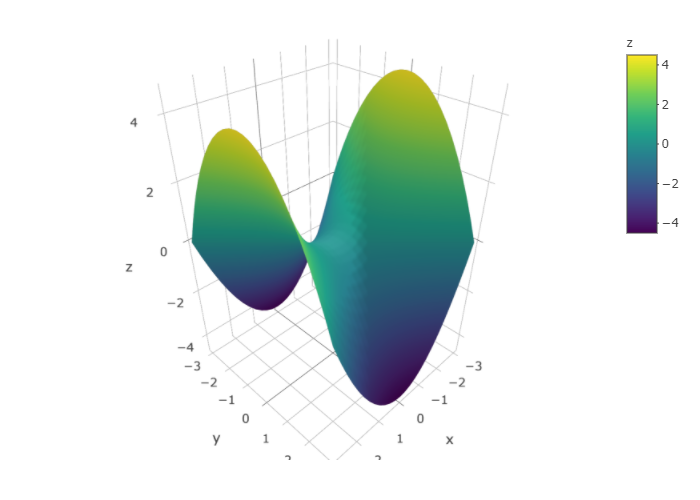
\includegraphics[width=0.8\linewidth]{resources/images/hyperboloide} 

}

\caption{Hyperboloïde : $z=(x^2-y^2)/2$}\label{fig:hyperboloide}
\end{figure}

\begin{figure}

{\centering 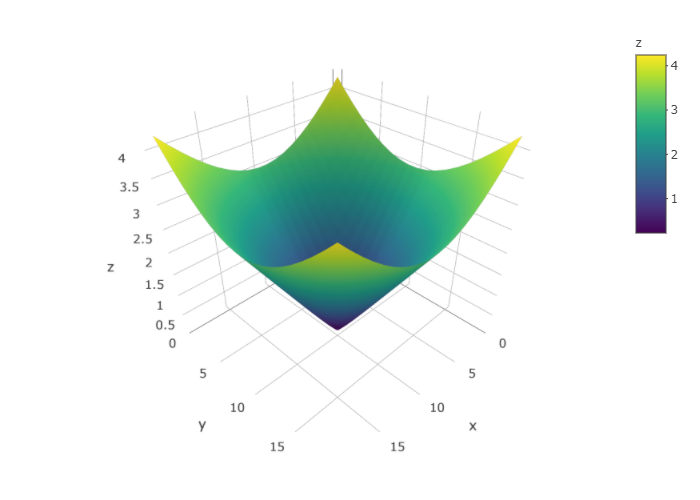
\includegraphics[width=0.8\linewidth]{resources/images/cone} 

}

\caption{Cône : $z=\sqrt{x^2+y^2}$}\label{fig:cone}
\end{figure}

\begin{figure}

{\centering 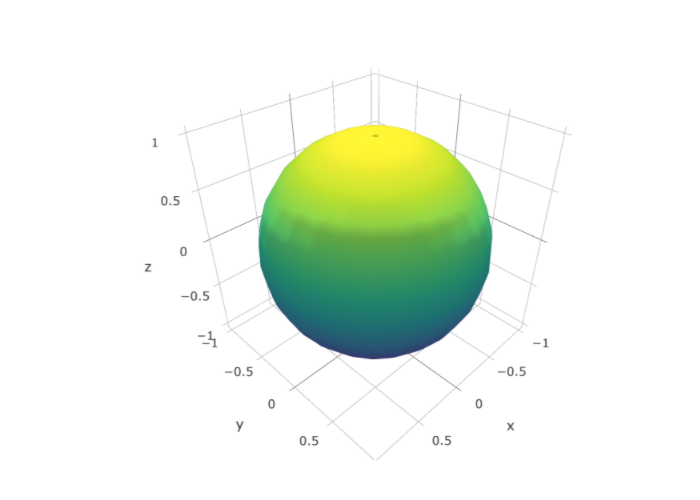
\includegraphics[width=0.8\linewidth]{resources/images/sphere} 

}

\caption{Sphère: $x^2+y^2+z^2=R^2$}\label{fig:sphere}
\end{figure}

\begin{figure}

{\centering 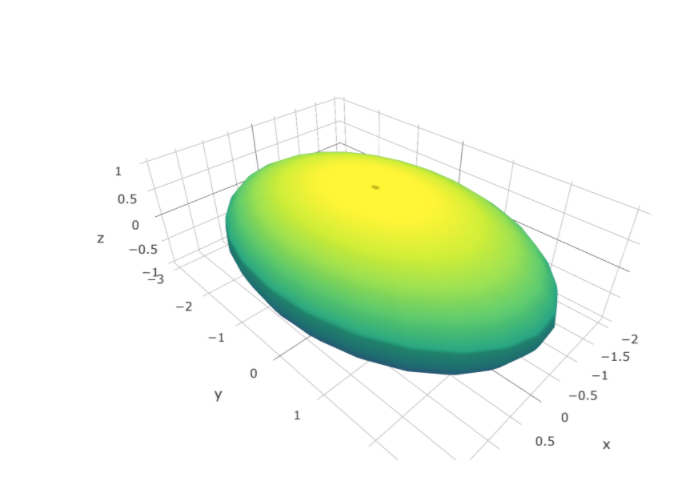
\includegraphics[width=0.8\linewidth]{resources/images/ellipse} 

}

\caption{Ellipse: $\dfrac{x^2}{a^2}+\dfrac{y^2}{b^2}+\dfrac{z^2}{c^2}=1$}\label{fig:ellipse}
\end{figure}

\begin{figure}

{\centering 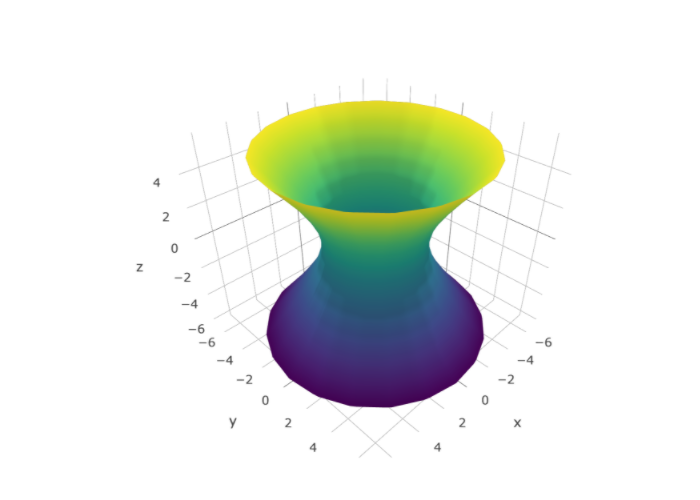
\includegraphics[width=0.8\linewidth]{resources/images/hyper1nappe} 

}

\caption{Hyperboloïde à une nappe: $\dfrac{x^2}{a^2}+\dfrac{y^2}{b^2}-\dfrac{z^2}{c^2}=1$}\label{fig:hyper1nappe}
\end{figure}

\begin{figure}

{\centering 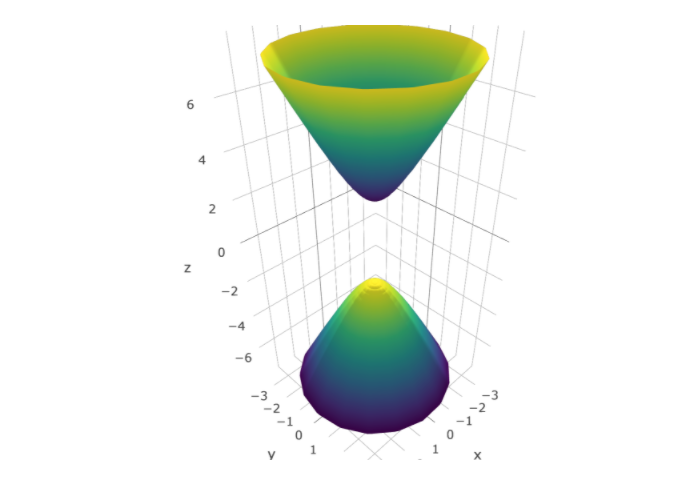
\includegraphics[width=0.8\linewidth]{resources/images/hyper2nappe} 

}

\caption{Hyperboloïde à deux nappes: $-\dfrac{x^2}{a^2}-\dfrac{y^2}{b^2}+\dfrac{z^2}{c^2}=1$}\label{fig:hyper2nappe}
\end{figure}

\begin{figure}

{\centering 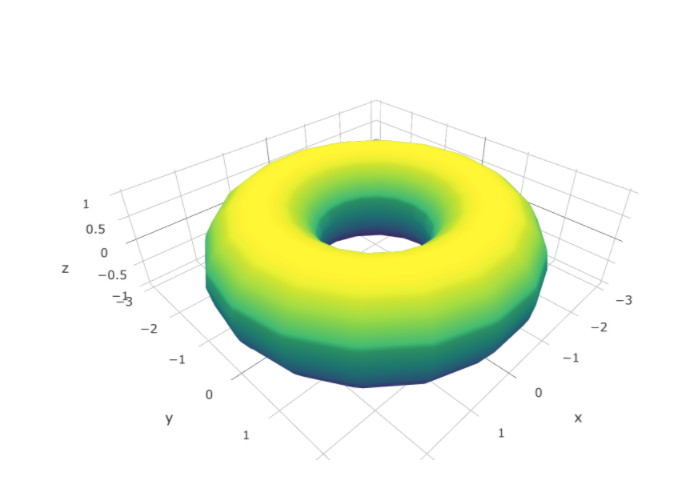
\includegraphics[width=0.8\linewidth]{resources/images/tore} 

}

\caption{Tore: $(x^2+y^2+z^2+a^2-r^2)^2=4 a^2(x^2+y^2)$}\label{fig:tore}
\end{figure}

\hypertarget{comment-etudier-les-graphiques-de-fonctions-de-deux-variables}{%
\section{Comment étudier les graphiques de fonctions de deux
variables}\label{comment-etudier-les-graphiques-de-fonctions-de-deux-variables}}

Comme vous avez pu voir dans les figures précédentes de la section
\ref{graphiques-divers}, les surfaces en trois dimensions peuvent être
complexes et difficiles à dessiner à la main. Pour tenter de nous aider
à représenter graphiquement ces fonctions, nous allons introduire deux
nouveaux outils: les coupes transversales et les courbes de niveaux.

\BeginKnitrBlock{remark}
\iffalse{} {Remarque. } \fi{}Lorsque vous vous trouvez dans la version
en ligne de ce document et que vous placez le curseur de votre souris
sur les figures précédentes, vous devriez apercevoir des lignes et des
courbes noires, centrées sur votre curseur. Ces lignes et courbes
correspondent aux coupes transversales et aux courbes de niveaux.
\EndKnitrBlock{remark}

\hypertarget{les-coupes-transversales}{%
\subsection{Les coupes transversales}\label{les-coupes-transversales}}

L'idée des coupes transversales est de fixer la valeur de l'une des deux
variables indépendantes. À ce moment, nous observons la fonction dans le
plan où est fixé la variable. Si nous fixons \(x=k\) où
\(k\in\mathbb{R}\), nous coupons la surface avec le plan \(x=k\). Nous
étudions donc une courbe dans le plan \(x=k\) et cette courbe se trouve
dans un espace à deux dimensions.

Pour bien visualiser les coupes transversales, nous vous invitons à
utiliser l'application
\href{https://www.geogebra.org/?lang=fr}{GeoGebra} de la section
\ref{geogebra-fctvar}.

\BeginKnitrBlock{example}
\protect\hypertarget{exm:unnamed-chunk-124}{}{\label{exm:unnamed-chunk-124}
}Dessinez les coupes transversales de la fonction \(z=f(x,y)=x^2+y\).
\EndKnitrBlock{example}

La figure \ref{fig:fctcoupe} représente la fonction \(f(x,y)\).

\begin{figure}

{\centering 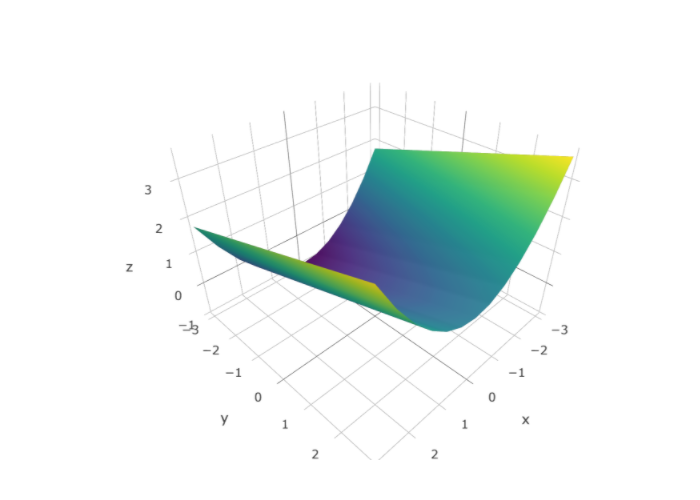
\includegraphics[width=0.8\linewidth]{resources/images/fct_coupe} 

}

\caption{Graphique de $f(x,y)=x^2+y$}\label{fig:fctcoupe}
\end{figure}

Déterminons tout d'abord les familles de courbes obtenues lorsque nous
fixons la valeur de la variable \(x\). Posons \(x=k\) où \(k\) est une
constante. Ainsi \(f(k,y)=z=k^2+y\). Donc dans le plan \(x=k\), l'allure
de la fonction est une droite d'équation \(z=y+k^2\), comme on peut le
voir à la figure \ref{fig:fctcoupe1}.

\begin{figure}

{\centering 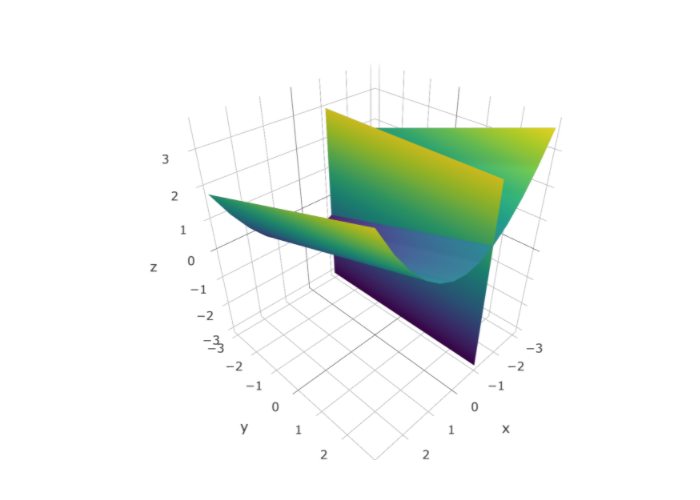
\includegraphics[width=0.8\linewidth]{resources/images/fct_coupe_plan1} 

}

\caption{Graphique de $f(x,y)=x^2+y$ et du plan $x=-1$}\label{fig:fctcoupe1}
\end{figure}

Déterminons maintenant les familles de courbes obtenues lorsque nous
fixons la valeur de la variable \(y\). Posons \(y=k\) où \(k\) est une
constante. Ainsi \(f(x,k)=z=x^2+k\). Donc dans le plan \(y=k\), l'allure
de la fonction est une parabole d'équation \(z=x^2+k\), comme on peut le
voir à la figure \ref{fig:fctcoupe2}.

\begin{figure}

{\centering 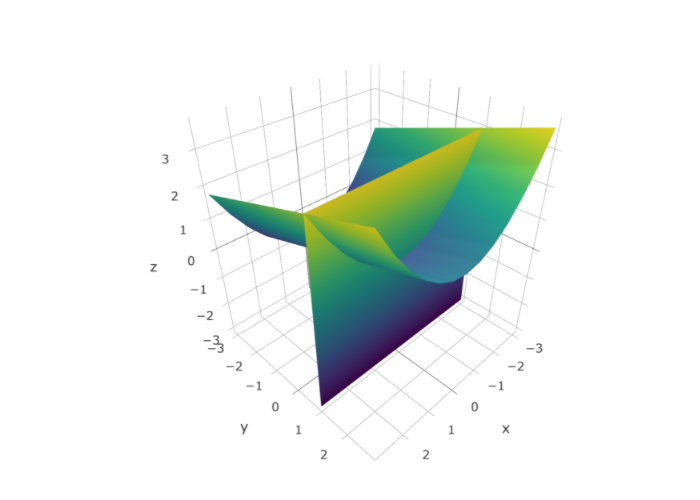
\includegraphics[width=0.8\linewidth]{resources/images/fct_coupe_plan2} 

}

\caption{Graphique de $f(x,y)=x^2+y$ et du plan $y=1$}\label{fig:fctcoupe2}
\end{figure}

\hypertarget{les-courbes-de-niveaux}{%
\subsection{Les courbes de niveaux}\label{les-courbes-de-niveaux}}

\BeginKnitrBlock{definition}[Courbes de niveaux]
\protect\hypertarget{def:unnamed-chunk-125}{}{\label{def:unnamed-chunk-125}
\iffalse (Courbes de niveaux) \fi{} }Soit une fonction définie par
\(z=f(x,y)\) et \(k\in\mathbb{R}\). La courbe de niveau \(k\) correspond
à l'ensemble des points \((x,y)\) tels que \(f(x,y)=k\).
\EndKnitrBlock{definition}

\BeginKnitrBlock{remark}
\iffalse{} {Remarque. } \fi{}Les courbes de niveaux correspondent donc à
une coupe transversale de la fonction lorsque nous fixons la variable
dépendante.
\EndKnitrBlock{remark}

\begin{quote}
La fonction est constante le long de ses courbes de niveaux.
\end{quote}

Les applications les plus répandues des courbes de niveaux sont dans les
cartes topographiques. Une carte topographique est une carte à échelle
réduite représentant le relief déterminé par altimétrie et les
aménagements humains d'une région géographique de manière précise et
détaillée sur un plan horizontal. La figure \ref{fig:montgreg}
représente une carte topographique du Mont Saint-Grégoire. Dans la
version en ligne de ce document, vous pouvez vous déplacer dans la carte
et aller voir le relief topographique ailleurs sur la planète.

\begin{figure}

{\centering 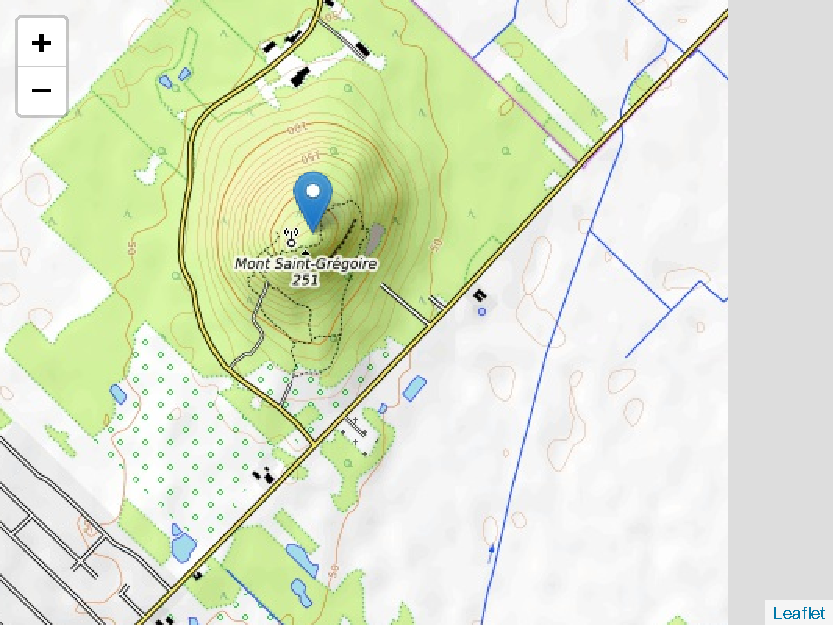
\includegraphics[width=0.8\linewidth]{calcul3_files/figure-latex/montgreg-1} 

}

\caption{Carte topographique du Mont Saint-Grégoire}\label{fig:montgreg}
\end{figure}

Un autre exemple de carte topographique peut être obtenu en utilisant
des données topographiques du volcan \textbf{Maunga Whau} situé dans la
région d'Auckland. Les données sont distribuées sur une grille de 10
mètres par 10 mètres. La figure \ref{fig:volcano3d} représente le volcan
en trois dimensions.

\begin{figure}

{\centering 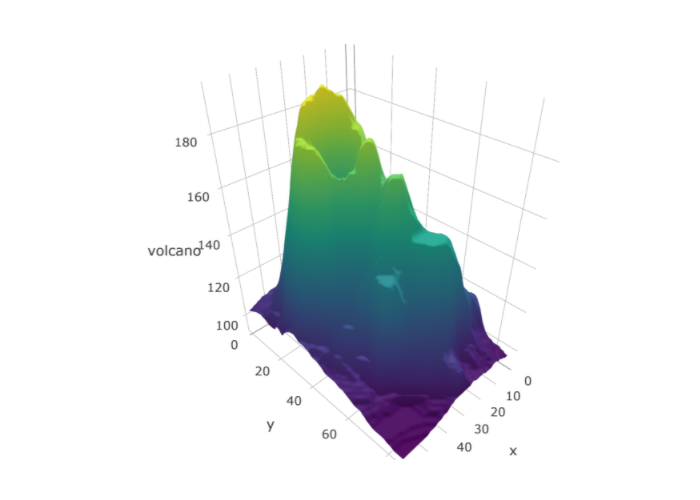
\includegraphics[width=0.8\linewidth]{resources/images/volcano} 

}

\caption{Représentation du volcan Maunga Whau}\label{fig:volcano3d}
\end{figure}

Nous pouvons représenter les courbes de niveaux de ce volcan comme à la
figure \ref{fig:volcano2d}.

\begin{figure}

{\centering 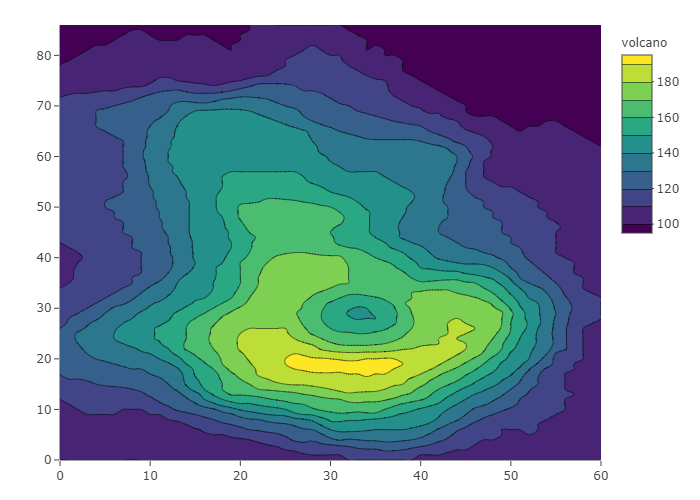
\includegraphics[width=0.8\linewidth]{resources/images/volcano-contour} 

}

\caption{Courbes de niveaux du volcan Maunga Whau}\label{fig:volcano2d}
\end{figure}

Faisons maintenant quelques exemples.

\BeginKnitrBlock{example}
\protect\hypertarget{exm:unnamed-chunk-127}{}{\label{exm:unnamed-chunk-127}
}Déterminez la nature des courbes de niveaux du paraboloïde
\(f(x,y)=x^2+y^2\). Dessinez quelques courbes de niveaux.
\EndKnitrBlock{example}
\vspace*{6cm}

\BeginKnitrBlock{example}
\protect\hypertarget{exm:unnamed-chunk-128}{}{\label{exm:unnamed-chunk-128}
}Trouvez les courbes de niveaux de la fonction \(f(x,y)=x^2-y\).
\EndKnitrBlock{example}
\vspace*{6cm}

\BeginKnitrBlock{example}
\protect\hypertarget{exm:unnamed-chunk-129}{}{\label{exm:unnamed-chunk-129}
}Trouvez les courbes de niveaux de la fonction \(f(x,y)=ye^{-|x|}\).
\EndKnitrBlock{example}
\vspace*{6cm}

\BeginKnitrBlock{example}
\protect\hypertarget{exm:unnamed-chunk-130}{}{\label{exm:unnamed-chunk-130}
}Trouvez les courbes de niveaux de la fonction \(f(x,y)=e^{x^2-y^2}\).
\EndKnitrBlock{example}
\vspace*{6cm}

\BeginKnitrBlock{example}
\protect\hypertarget{exm:unnamed-chunk-131}{}{\label{exm:unnamed-chunk-131}
}Trouvez les courbes de niveaux de la fonction
\(f(x,y)=\ln(4-x^2-4y^2)\).
\EndKnitrBlock{example}
\vspace*{6cm}

\hypertarget{domaine}{%
\section{Domaine}\label{domaine}}

\BeginKnitrBlock{definition}[Domaine d'une fonction]
\protect\hypertarget{def:unnamed-chunk-132}{}{\label{def:unnamed-chunk-132}
\iffalse (Domaine d'une fonction) \fi{} }Le domaine d'une fonction
réelle \(f(x_1,\ldots,x_n)\) (ou domaine de définition d'une fonction),
noté \(\text{dom} f\), est un sous ensemble de \(\mathbb{R^n}\) qui
contient toutes les valeurs de \(x_i\) avec \(i=1,\ldots, n\), pour
lesquelles la règle de correspondance de \(f(x_1,\ldots,x_n)\) est
définie.
\EndKnitrBlock{definition}

Pour déterminer le domaine d'une fonction réelle \(f(x_1,\ldots,x_n)\),
il suffit de suivre les étapes suivantes:

\begin{enumerate}
\def\labelenumi{\arabic{enumi}.}
\tightlist
\item
  Vérifier si \(f(x_1,\ldots,x_n)\) est définie dans un contexte, afin
  de voir si celui-ci restreint les valeurs des variables indépendantes.
\item
  Enlever les valeurs des variables indépendantes qui annulent le
  dénominateur.
\item
  L'argument des racines paires doit être plus grand ou égal à zéro,
  c'est-à-dire \(\geq 0\).
\item
  L'argument des logarithmes doit être \textbf{strictement} plus grand
  que zéro, c'est-à-dire \(> 0\).
\item
  Les fonctions trigonométriques usuelles ont souvent des dénominateurs,
  par exemple \(\tan\), \(\cot\), \(\csc\) et \(\sec\). De plus, les
  fonctions trigonométriques inverses ont souvent des domaines
  restreints.
\end{enumerate}

Voici quelques exemples.

\BeginKnitrBlock{example}
\protect\hypertarget{exm:unnamed-chunk-133}{}{\label{exm:unnamed-chunk-133}
}Déterminez le domaine des fonctions suivantes:

\begin{enumerate}
\def\labelenumi{\alph{enumi}.}
\tightlist
\item
  \(f(x,y)=x^2+y^2\)
\item
  \(f(x,y)=\dfrac{1}{9-x^2-y^2}\)
\item
  \(f(x,y)=\dfrac{\sqrt{9-x^2-y^2}}{x-y}\)
\item
  \(f(x,y)=\ln(4-x^2-4y^2)\)
\item
  \(f(x,y)=\sqrt{x^2+y^2-1}+\sqrt{4-x^2-y^2}\)
\item
  \(f(x,y)=\sqrt{x(1-|y|)}\)
\item
  \(f(x,y)=\dfrac{xy}{x^2-y^2}\)
\item
  \(f(x,y)=\dfrac{1}{\sqrt{x^2-y^2}}\)
\end{enumerate}
\EndKnitrBlock{example}
\vspace*{20cm}

\hypertarget{limites}{%
\section{Limites}\label{limites}}

Nous allons débuter en rappelant la définition de la limite d'une
fonction à une variable.

\BeginKnitrBlock{definition}[Limite d'une fonction à une variable]
\protect\hypertarget{def:unnamed-chunk-134}{}{\label{def:unnamed-chunk-134}
\iffalse (Limite d'une fonction à une variable) \fi{} }Soit une fonction
\(f(x)\). Nous disons que \(L\) est la limite de \(f(x)\) lorsque \(x\)
tend vers \(a\) si pour tout \(\epsilon >0\), il existe \(\delta\) tel
que si \(|x-a|<\delta\) alors \(|f(x)-L|<\epsilon\). Nous notons alors:
\[ \lim_{x\to a} f(x) = L \]
\EndKnitrBlock{definition}

\textbf{WIP}

\BeginKnitrBlock{proposition}[Les propriétés des limites]
\protect\hypertarget{prp:unnamed-chunk-135}{}{\label{prp:unnamed-chunk-135}
\iffalse (Les propriétés des limites) \fi{} }Soit \(f(x,y)\) et
\(g(x,y)\) deux fonctions de deux variables.

\begin{align*}
& \lim_{(x,y)\to(a,b)}f(x,y)\pm g(x,y)=\lim_{(x,y)\to(a,b)}f(x,y)\pm \lim_{(x,y)\to(a,b)} g(x,y) \\
& \lim_{(x,y)\to(a,b)}f(x,y)\cdot  g(x,y)=\lim_{(x,y)\to(a,b)}f(x,y)\cdot \lim_{(x,y)\to(a,b)} g(x,y) \\
& \lim_{(x,y)\to(a,b)}\dfrac{f(x,y)}{g(x,y)}=\dfrac{\lim\limits_{(x,y)\to(a,b)}f(x,y)}{ \lim\limits_{(x,y)\to(a,b)} g(x,y)}\quad \text{si $g(x,y)\neq 0$ près de $(a,b)$}
\end{align*}
\EndKnitrBlock{proposition}

\BeginKnitrBlock{example}
\protect\hypertarget{exm:unnamed-chunk-136}{}{\label{exm:unnamed-chunk-136}
}Trouvez la limite suivante:

\[
\lim_{(x,y)\to(1,2)} (x^2+y)
\]
\EndKnitrBlock{example}

\BeginKnitrBlock{example}
\protect\hypertarget{exm:lim-sin-sur-x}{}{\label{exm:lim-sin-sur-x} }Trouvez
la limite suivante:

\[
\lim_{(x,y)\to(0,0)}\dfrac{\sin (x^2+y^2)}{x^2+y^2}
\]
\EndKnitrBlock{example}

Nous avons pu lever l'indétermination de l'exemple
\ref{exm:lim-sin-sur-x} en utilisant une limite vue dans un cours de
calcul intégral. Malheureusement, il sera habituellement plus difficile
de lever des indéterminations. En particulier, il n'existe pas
d'analogue à la règle de L'Hospital pour des fonctions de deux variables
ou plus.

Nous verrons par contre deux techniques pour être en mesure de calculer
des limites de fonctions de deux variables ou plus: la méthode des
chemins et la méthode du gendarme.

\hypertarget{la-methode-des-chemins}{%
\subsection{La méthode des chemins}\label{la-methode-des-chemins}}

Cette méthode est une généralisation du principe de la limite à droite
et de la limite à gauche. Lorsque nous avons:

\[ \lim_{x\to a} f(x) \]

cela signifie que la valeur de \(x\) s'approche de \(a\). La variable
\(x\) peut s'approcher de \(a\) de deux façons différentes, par la
droite ou par la gauche. Dans le cas de la limite suivante:

\[ \lim_{(x,y)\to (a,b)} f(x,y) \]

cela signifie que nous devons nous approcher du point \((a,b)\). Par
contre, il existe plus de deux façons de se rendre au point \((a,b)\).
Il en existe en fait une infinité! La figure \ref{fig:limites2d-3d}
présente une représentation d'une limite pour une fonction d'une seule
variable dans la figure de gauche. Dans la figure de droite, nous
montrons trois chemins possibles, parmi l'infinité de chemins possibles.

\begin{figure}

{\centering 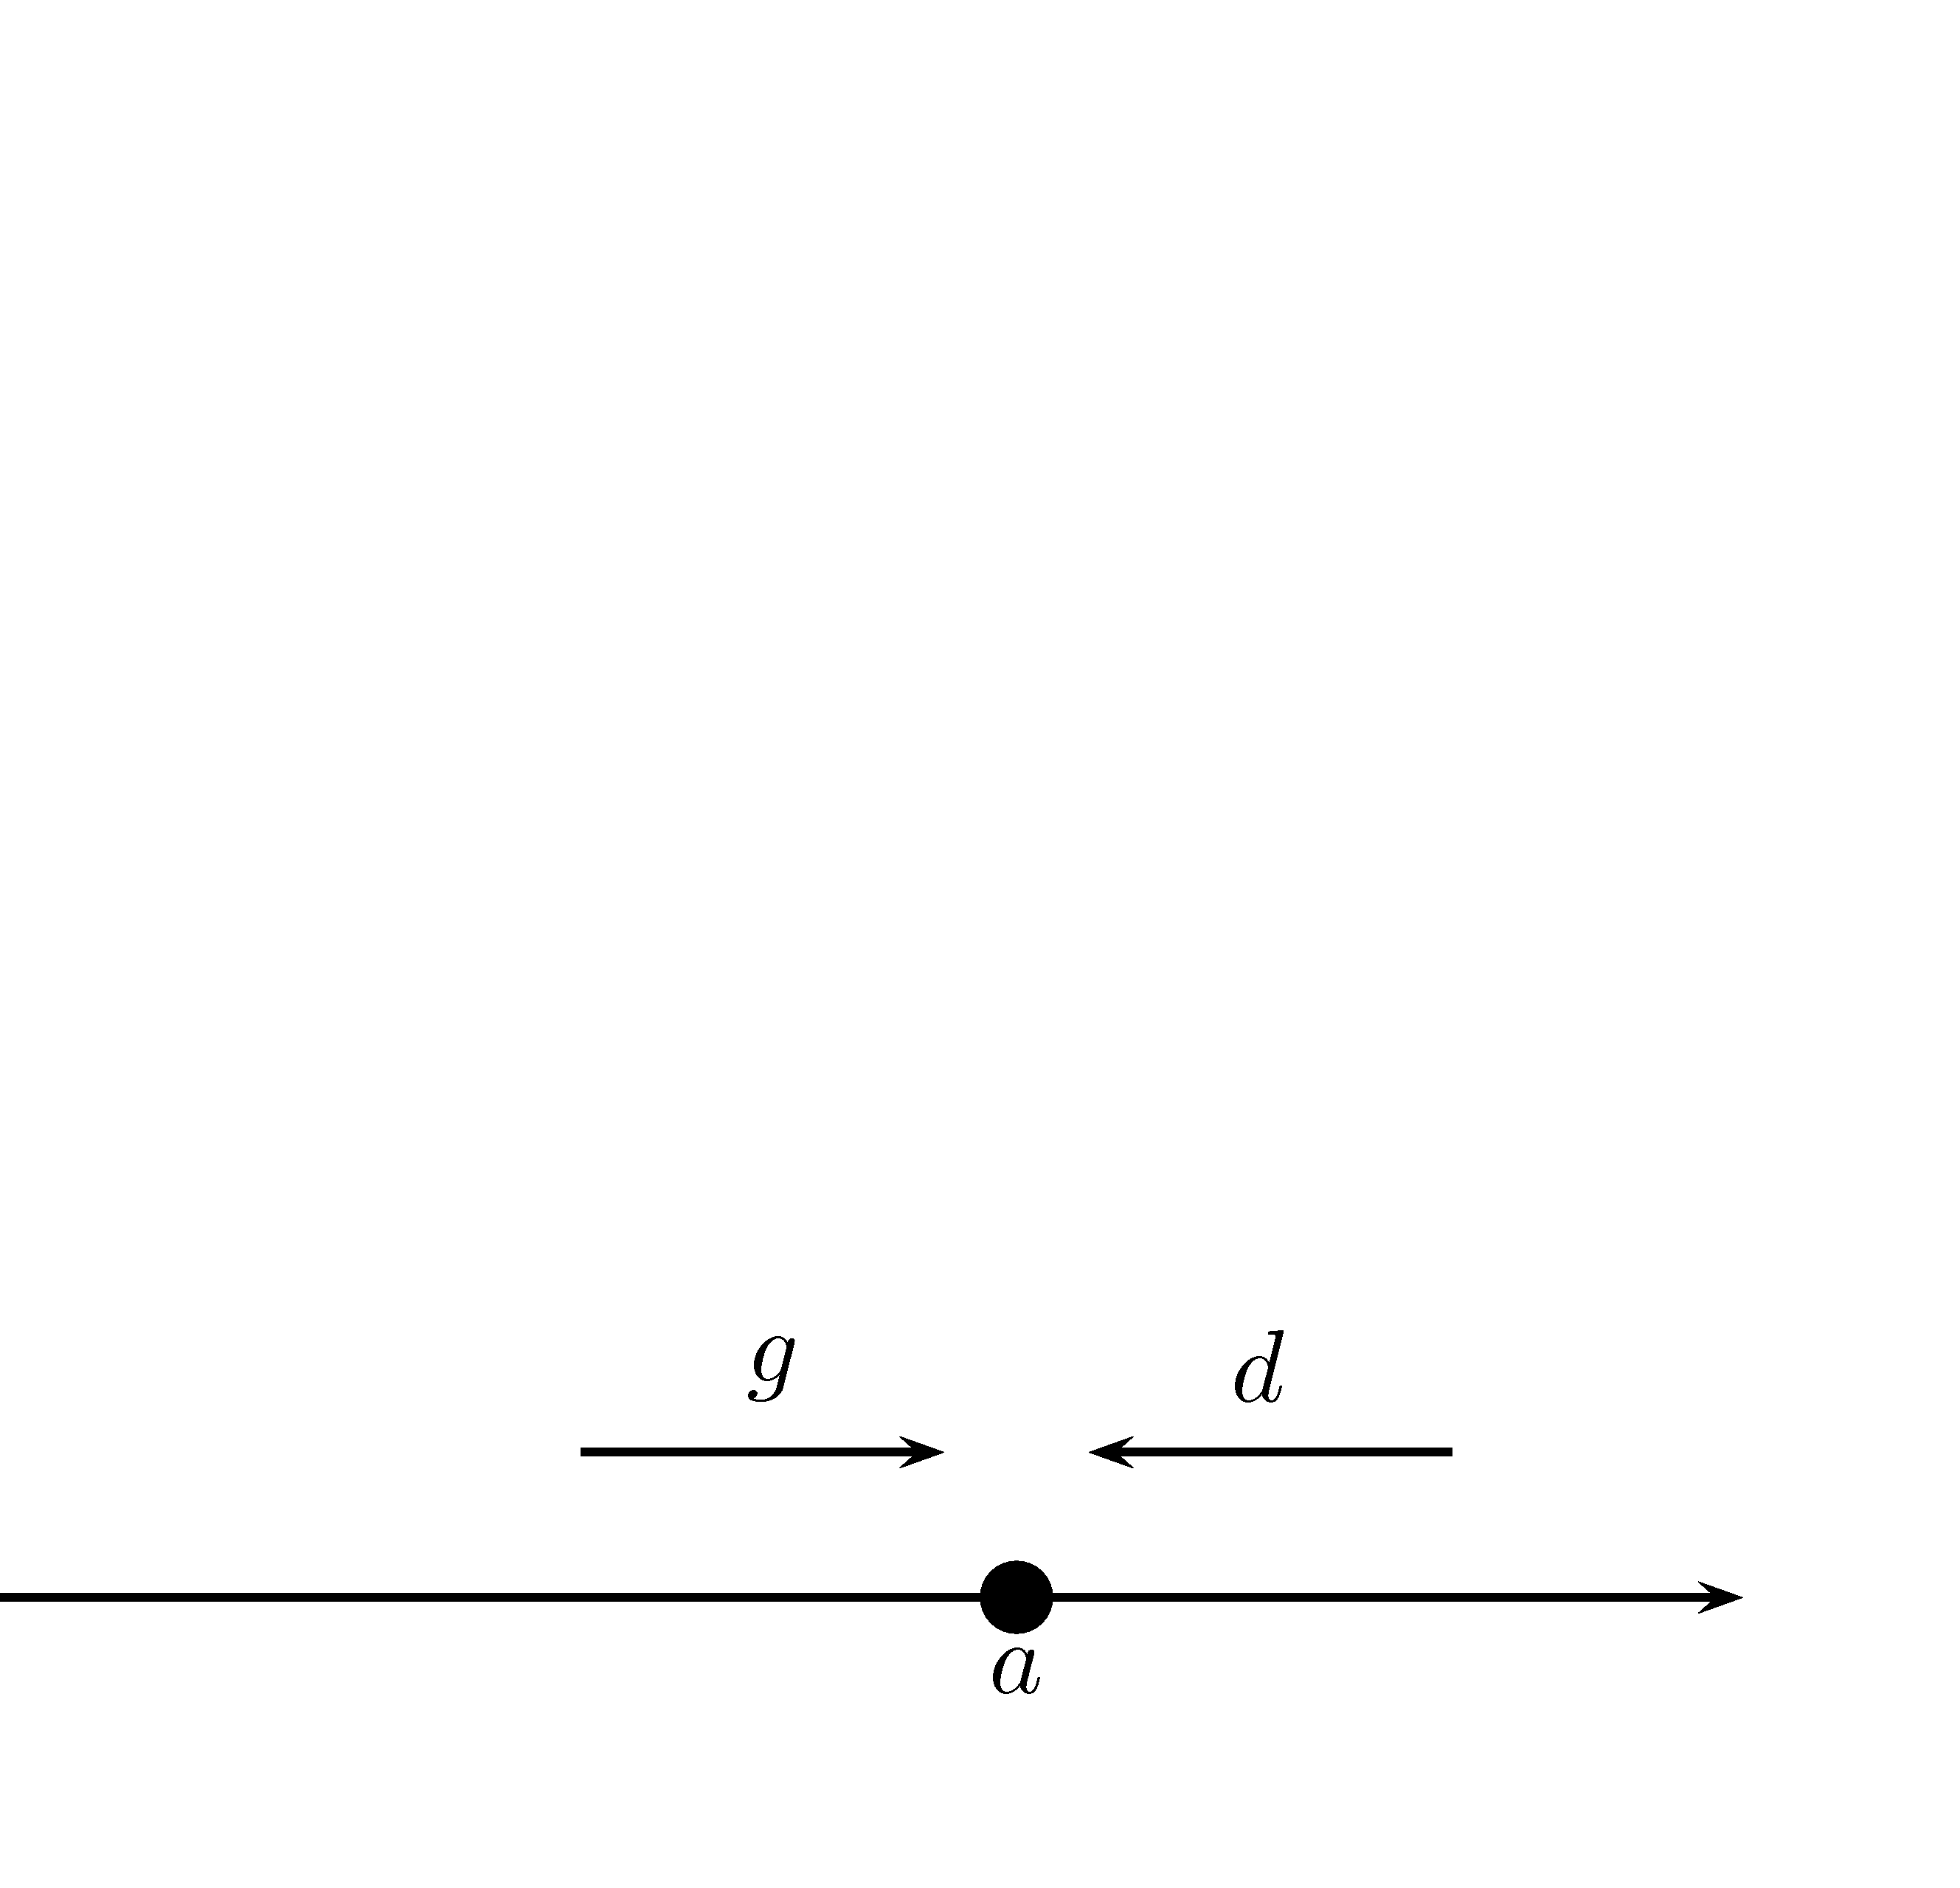
\includegraphics[width=0.45\linewidth]{resources/images/latex/limite2d} 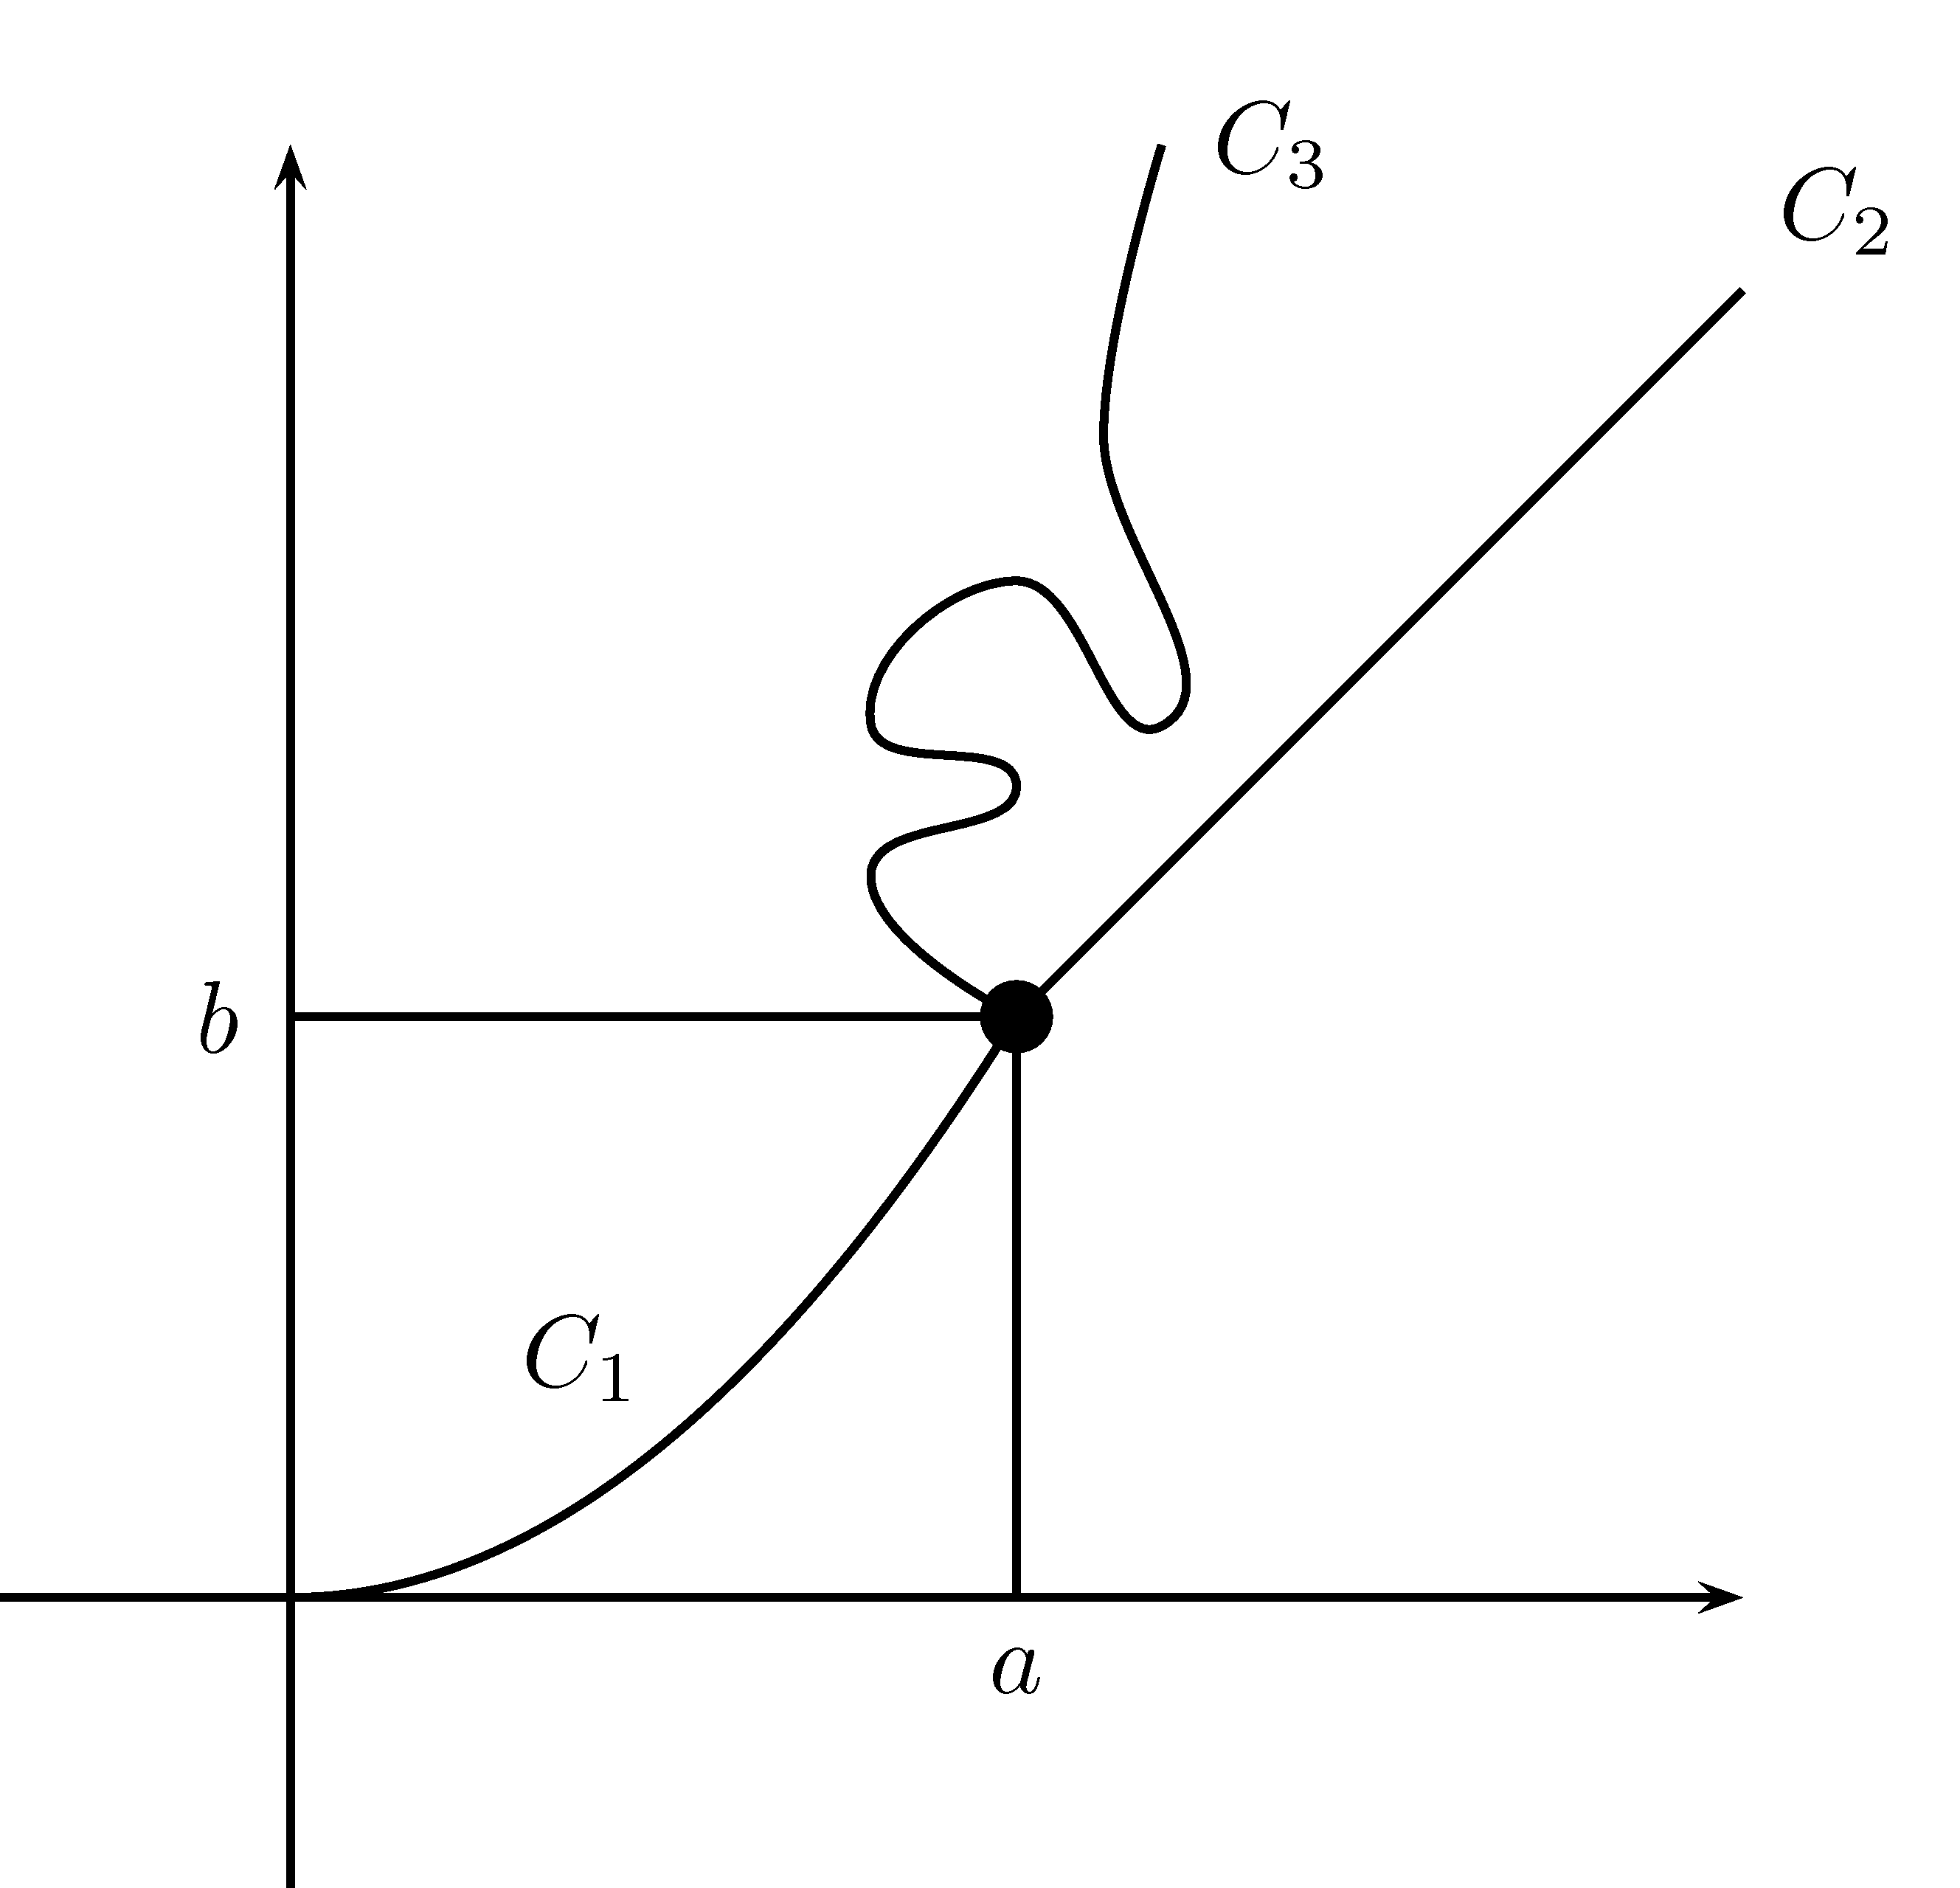
\includegraphics[width=0.45\linewidth]{resources/images/latex/limite3d} 

}

\caption{Représentation d'une limite en deux dimensions et d'une autre en trois dimensions.}\label{fig:limites2d-3d}
\end{figure}

\BeginKnitrBlock{example}
\protect\hypertarget{exm:unnamed-chunk-137}{}{\label{exm:unnamed-chunk-137}
}Déterminez, si elle existe, la limite suivante:

\[ \lim_{(x,y)\to (0,0)}\dfrac{x^2}{x^2+y^2} \]
\EndKnitrBlock{example}

En général, nous désirons trouver la limite en \((0,0)\) et nous allons
tester les chemins suivants:

\begin{itemize}
\tightlist
\item
  \(x=0\)
\item
  \(y=0\)
\item
  \(y=x\)
\item
  \(y=kx\) où \(k\) est une constante
\item
  \(y=kx^2\) où \(k\) est une constante
\end{itemize}

\BeginKnitrBlock{remark}
\iffalse{} {Remarque. } \fi{}La méthode des chemins ne permet que de
démontrer qu'une limite \textbf{n'existe pas}.
\EndKnitrBlock{remark}

\BeginKnitrBlock{example}
\protect\hypertarget{exm:unnamed-chunk-139}{}{\label{exm:unnamed-chunk-139}
}Déterminez, si elle existe, la limite suivante:

\[ \lim_{(x,y)\to (0,0)}\dfrac{xy}{x^2+y^2} \]
\EndKnitrBlock{example}

\BeginKnitrBlock{example}
\protect\hypertarget{exm:unnamed-chunk-140}{}{\label{exm:unnamed-chunk-140}
}Déterminez, si elle existe, la limite suivante:

\[ \lim_{(x,y)\to (0,0)}\dfrac{xy^2}{x^2+y^4} \]
\EndKnitrBlock{example}

\BeginKnitrBlock{example}
\protect\hypertarget{exm:unnamed-chunk-141}{}{\label{exm:unnamed-chunk-141}
}Déterminez, si elle existe, la limite suivante:

\[ \lim_{(x,y)\to (0,0)}\dfrac{x^2+y^2}{y} \]
\EndKnitrBlock{example}

\hypertarget{la-methode-des-gendarmes}{%
\subsection{La méthode des gendarmes}\label{la-methode-des-gendarmes}}

Puisque la méthode des chemins ne nous permet pas de démontrer qu'une
limite existe, nous allons introduire la méthode des gendarmes, qui elle
permet de démontrer qu'une limite existe. Nous débutons pas utiliser la
méthode des chemins pour calculer la limite:

\[ \lim_{(x,y)\to (a,b)}f(x,y) \]

Si tous les chemins nous donnent une limite égale à \(L\), nous pouvons
présumer que:

\[ \lim_{(x,y)\to (a,b)}f(x,y)=L \]

Nous voulons maintenant trouver une fonction \(M(x,y)\) telle que:

\[ 0 \leq |f(x,y)-L| \leq M(x,y) \]

et telle que la limite suivante est vérifiée:

\[ \lim_{(x,y)\to (a,b)} M(x,y) = 0 \]

Nous nous retrouvons donc dans la situation suivante:

\begin{align*}
0 &\leq |f(x,y)-L| &\leq M(x,y) \\
\lim_{(x,y)\to (a,b)} 0 &\leq \lim_{(x,y)\to (a,b)}|f(x,y)-L| &\leq \lim_{(x,y)\to (a,b)}M(x,y) \\
0 &\leq \lim_{(x,y)\to (a,b)}|f(x,y)-L| &\leq 0
\end{align*}

Nous pouvons donc conclure que:

\[ \lim_{(x,y)\to (a,b)}f(x,y)=L \]

Pour utiliser la méthode des gendarmes, nous utiliserons à plusieurs
reprises l'inégalité suivante.

\BeginKnitrBlock{proposition}
\protect\hypertarget{prp:unnamed-chunk-142}{}{\label{prp:unnamed-chunk-142}
}Soit \(x\) et \(y\) deux nombres réels. Nous avons: \begin{align*}
\left|\dfrac{x^2}{x^2+y^2}\right| &\leq 1 \\
\left|\dfrac{y^2}{x^2+y^2}\right| &\leq 1
\end{align*}
\EndKnitrBlock{proposition}

\BeginKnitrBlock{proof}
\iffalse{} {Preuve. } \fi{}Nous avons: \begin{align*}
x^2 &\leq x^2+y^2 \\
\dfrac{x^2}{x^2+y^2} &\leq 1
\end{align*} L'autre inégalité se démontre de la même manière.
\EndKnitrBlock{proof}

\BeginKnitrBlock{example}
\protect\hypertarget{exm:unnamed-chunk-144}{}{\label{exm:unnamed-chunk-144}
}Trouvez la limite suivante:
\[ \lim_{(x,y)\to (0,0)}\dfrac{x^2y}{x^2+y^2} \]
\EndKnitrBlock{example}

\BeginKnitrBlock{example}
\protect\hypertarget{exm:unnamed-chunk-145}{}{\label{exm:unnamed-chunk-145}
}Trouvez la limite suivante:
\[ \lim_{(x,y)\to (0,0)}\dfrac{y^3}{x^2+y^2} \]
\EndKnitrBlock{example}

\hypertarget{exercises-divers-de-limites}{%
\subsection{Exercises divers de
limites}\label{exercises-divers-de-limites}}

\BeginKnitrBlock{example}
\protect\hypertarget{exm:unnamed-chunk-146}{}{\label{exm:unnamed-chunk-146}
}Trouvez, si possible, les limites suivantes:

\begin{enumerate}
\def\labelenumi{\alph{enumi}.}
\tightlist
\item
  \(\lim_{(x,y)\to (2,-1)} (xy+y^2)\)
\item
  \(\lim_{(x,y)\to (0,0)} \sqrt{x^2+y^2}\)
\item
  \(\lim_{(x,y)\to (0,0)} \dfrac{x}{x^2+y^2}\)
\item
  \(\lim_{(x,y)\to (0,0)} \dfrac{\cos(xy)}{1-x-\cos(y)}\)
\item
  \(\lim_{(x,y)\to (0,1)} \dfrac{x^2(y-1)^2}{x^2+(y-1)^2}\)
\item
  \(\lim_{(x,y)\to (0,0)} \dfrac{\sin(x-y)}{\cos(x+y)}\)
\item
  \(\lim_{(x,y)\to (0,0)} \dfrac{\sin(xy)}{x^2+y^2}\)
\end{enumerate}
\EndKnitrBlock{example}

\hypertarget{la-continuite}{%
\section{La continuité}\label{la-continuite}}

La notion de continuité pour les fonctions de plusieurs variables est
similaire à celle des fonctions d'une seule variable.

\BeginKnitrBlock{definition}[Continuité pour les fonctions de deux variables]
\protect\hypertarget{def:unnamed-chunk-147}{}{\label{def:unnamed-chunk-147}
\iffalse (Continuité pour les fonctions de deux variables) \fi{} }Soit
une fonction \(f(x,y)\) et un point \((a,b)\in\text{dom} f\). Nous
disons que \(f(x,y)\) est continue au point \((a,b)\) si:
\[ \lim_{(x,y)\to (a,b)} f(x,y) = f(a,b) \]
\EndKnitrBlock{definition}

\begin{quote}
Cette définition se généralise facilement aux fonctions de trois
variables ou plus.
\end{quote}

\BeginKnitrBlock{example}
\protect\hypertarget{exm:unnamed-chunk-148}{}{\label{exm:unnamed-chunk-148}
}Déterminez si la fonction suivante:

\[ 
f(x,y) = \begin{cases}
\dfrac{x^2y}{x^2+y^2} & \text{si } (x,y)\neq (0,0) \\
0 & \text{si } (x,y)= (0,0)
\end{cases}
\] est continue en \((0,0)\).
\EndKnitrBlock{example}

\BeginKnitrBlock{example}
\protect\hypertarget{exm:unnamed-chunk-149}{}{\label{exm:unnamed-chunk-149}
}Comment la fonction \(f(x,y)=\dfrac{x^2+y^2-x^3y^3}{x^2+y^2}\) définie
pour tous les \((x,y)\neq (0,0)\) peut-elle être définie à l'origine
pour qu'elle soit continue partout sur \(\mathbb{R}^2\)?
\EndKnitrBlock{example}

\BeginKnitrBlock{example}
\protect\hypertarget{exm:unnamed-chunk-150}{}{\label{exm:unnamed-chunk-150}
}Comment la fonction \(f(x,y)=\dfrac{x^3-y^3}{x-y}\) définie pour tous
les \(x\neq y\) peut-elle être définie à l'origine pour qu'elle soit
continue partout sur \(\mathbb{R}^2\)?
\EndKnitrBlock{example}

\BeginKnitrBlock{example}
\protect\hypertarget{exm:unnamed-chunk-151}{}{\label{exm:unnamed-chunk-151}
}Déterminez si la fonction suivante:

\[ 
f(x,y) = \begin{cases}
\sin\left(\dfrac{x}{y}\right) & \text{si } x\neq 0 \text{ et } y\neq 0 \\
1 & \text{si } x= 0 \text{ et } y= 0
\end{cases}
\] est continue en \((0,0)\).
\EndKnitrBlock{example}

\hypertarget{geogebra-fctvar}{%
\section{Geogebra}\label{geogebra-fctvar}}

\hypertarget{applet_container}{}

\newpage

\hypertarget{pages-supplementaires-3}{%
\section{Pages supplémentaires}\label{pages-supplementaires-3}}

Des pages blanches supplémentaires pour ajouter, potentiellement, de
nouveaux exemples et exercices.

\multido{\i=1+1}{4}{
\newpage
\mbox{}
}

\hypertarget{derivfctvars}{%
\chapter{La dérivation de fonctions de plusieurs
variables}\label{derivfctvars}}

Vous trouverez à la section \ref{geogebra-derivfctvar} une application
\href{https://www.geogebra.org/?lang=fr}{GeoGebra} vous permettant de
visualiser des dérivées partielles et des dérivées directionnelles de
fonctions. À noter que cette application n'est disponible que dans la
version en ligne de ce document.

\hypertarget{introduction-4}{%
\section{Introduction}\label{introduction-4}}

Nous sommes maintenant prêts à aborder la notion de dérivée pour les
fonctions de deux variables ou plus.

\hypertarget{les-derivees-partielles}{%
\section{Les dérivées partielles}\label{les-derivees-partielles}}

Nous allons débuter en rappelant la définition de la dérivée d'une
fonction d'une seule variable.

\BeginKnitrBlock{definition}[Dérivée d'une fonction d'une seule variable]
\protect\hypertarget{def:unnamed-chunk-153}{}{\label{def:unnamed-chunk-153}
\iffalse (Dérivée d'une fonction d'une seule variable) \fi{} }Soit
\(f(x)\) une fonction. La dérivée de la fonction \(f(x)\), notée
\(f'(x)\) ou \(\dfrac{df}{dx}\) est donnée par:
\[ \lim_{\Delta x \to 0} \dfrac{f(x+\Delta x)-f(x)}{\Delta x} \]
\EndKnitrBlock{definition}

Nous savons que la dérivée d'une fonction correspond, entre autres, à la
pente de la droite tangente. Dans le cas d'une fonction de plus d'une
variable, la notion de pente de droite tangente en un point n'existe pas
à priori. Nous devrons donc définir une nouvelle définition de dérivée.

Nous allons débuter par introduire la notion de dérivée pour les
fonctions de deux variables. La généralisation pour les fonctions de
plus de deux variables se fait facilement.

Soit une fonction \(z=f(x,y)\). Pour étudier les deux (une par variable
indépendante) dérivées partielles de cette fonction, nous allons les
variations de cette fonction.

Supposons que nous nous trouvons dans un plan où la variable \(y\) est
constante. Ceci signifie que seule la variable \(x\) varie, c'est-à-dire
que nous partons du point \((x,y)\) jusqu'au point \((x+\Delta x,y)\).
Puisque nous avons deux points, nous pouvons déterminer le taux de
variation de la fonction \(f(x,y)\) par rapport à la vraible \(x\). Ce
taux est donné par:

\[  \dfrac{f(x+\Delta x,y)-f(x,y)}{\Delta x} \]

Lorsque nous prenons la limite de ce taux de variation lorsque
\(\Delta x\) tend vers \(0\), nous obtenons la dérivée partielle de
\(f(x,y)\) par rapport à \(x\). Mathématiquement, nous écrivons:

\[ \dfrac{\partial f}{\partial x}=\lim_{\Delta x \to 0} \dfrac{f(x+\Delta x,y)-f(x,y)}{\Delta x} \]

D'une manière similaire, nous pouvons définir la dérivée partielle de
\(f(x,y)\) par rapport à \(y\):

\[ \dfrac{\partial f}{\partial y}=\lim_{\Delta y \to 0} \dfrac{f(x,y+\Delta y)-f(x,y)}{\Delta y} \]

Géométriquement, la dérivée partielle de \(f(x,y)\) par rapport à \(x\)
correspond à la pente de la droite tangente à la courbe engendrée par
l'intersection du plan \(y=k\) où \(k\) est une constante et la surface
\(z=f(x,y)\).

La figure \ref{fig:derivee-partielle-x} représente dans l'image de
gauche la surface \(z=f(x,y)\) coupée par le plan \(y=k\) où \(k\) est
une constante. Nous apercevons l'intersection de la surface et du plan,
représentée par une courbe parabolique. La ligne pointillée représente
la droite tangente à la surface dans le plan \(y=k\). La figure de
droite représente la fonction parabolique dans le plan \(y=k\) ainsi que
la droite tangente.

\begin{figure}

{\centering 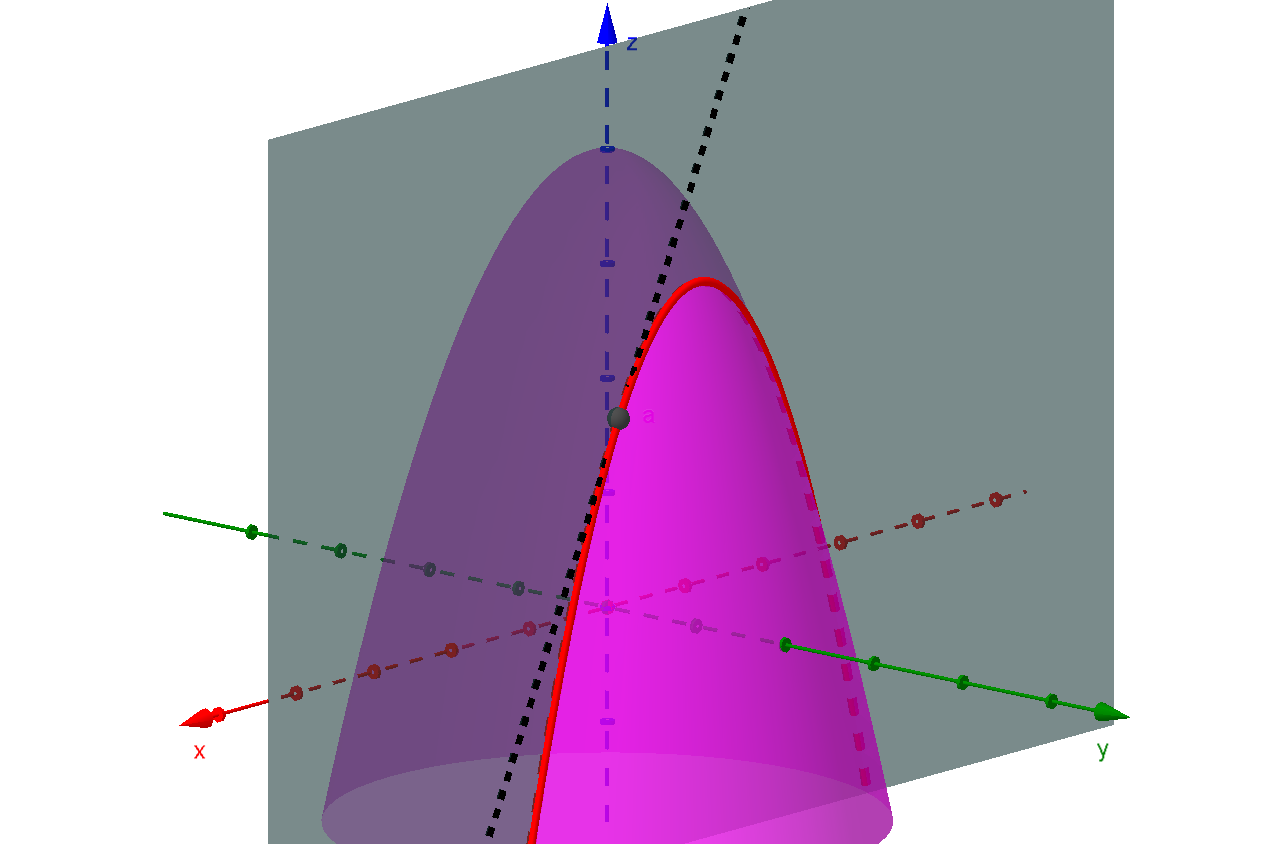
\includegraphics[width=0.5\linewidth]{resources/images/geogebra/deriveepartiellex3d} 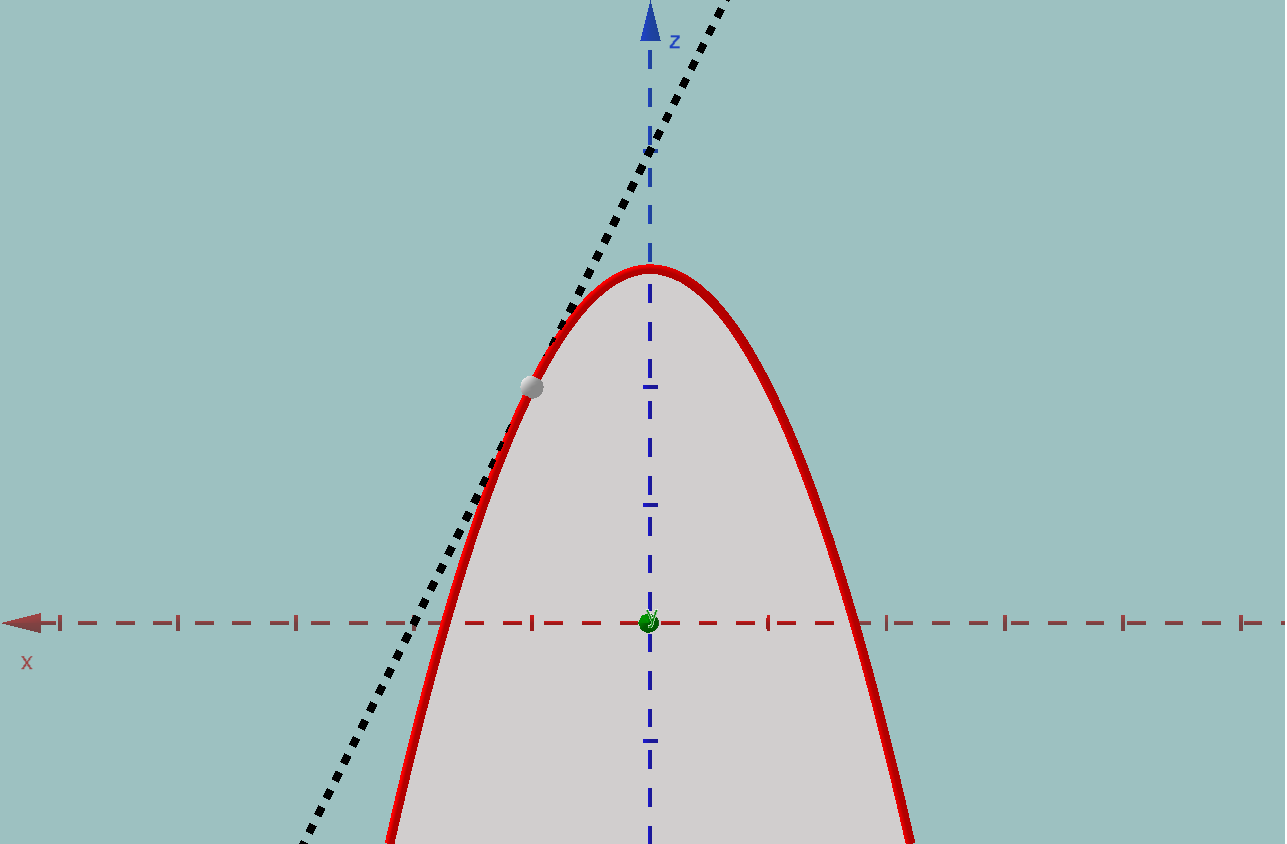
\includegraphics[width=0.5\linewidth]{resources/images/geogebra/deriveepartiellex2d} 

}

\caption{Représentation géométrique de la dérivée partielle de $f(x,y)$ par rapport à $x$}\label{fig:derivee-partielle-x}
\end{figure}

C'est la même correspondance pour \(\dfrac{\partial f}{\partial y}\), il
suffit d'étudier la courbe dans le plan \(x=k\) où \(k\) est une
constante.

\begin{quote}
Lorsque nous trouvons la dérivée partielle d'une fonction
\(f(x_1,x_2,\ldots,x_n)\) par rapport à la variable indépendante
\(x_i\), nous supposons toutes les autres variables indépendantes
\(x_j\) où \(j\neq i\) sont des constantes.
\end{quote}

\BeginKnitrBlock{proposition}[Notation pour dérivées partielles]
\protect\hypertarget{prp:unnamed-chunk-154}{}{\label{prp:unnamed-chunk-154}
\iffalse (Notation pour dérivées partielles) \fi{} }Soit une fonction
\(f(x_1,x_2,\ldots,x_n)\). La dérivée partielle de \(f\) par rapport à
la variable \(x_i\) peut être notée par:

\begin{itemize}
\tightlist
\item
  \(f_{x_i}\)
\item
  \(f_i\)
\item
  \(\dfrac{\partial f}{\partial x_i}\)
\item
  \(D_i f\)
\end{itemize}

Dans le cas où la fonction ne possède que deux variable, c'est-à-dire
une fonction \(f(x,y)\), nous pouvons noter la dérivée partielle de
\(f\) par rapport à \(x\) par:

\begin{itemize}
\tightlist
\item
  \(f_{x}\)
\item
  \(\dfrac{\partial f}{\partial x}\)
\item
  \(D_x f\)
\end{itemize}
\EndKnitrBlock{proposition}

\BeginKnitrBlock{example}
\protect\hypertarget{exm:unnamed-chunk-155}{}{\label{exm:unnamed-chunk-155}
}Trouvez les dérivées partielles de \(f(x,y)=x\cos(x+y^2)\).
\EndKnitrBlock{example}
\vspace*{8cm}

\BeginKnitrBlock{example}
\protect\hypertarget{exm:unnamed-chunk-156}{}{\label{exm:unnamed-chunk-156}
}Trouvez les dérivées partielles de \(f(x,y)=x^2\sin(y)\).
\EndKnitrBlock{example}
\vspace*{8cm}

\BeginKnitrBlock{example}
\protect\hypertarget{exm:unnamed-chunk-157}{}{\label{exm:unnamed-chunk-157}
}Trouvez les dérivées partielles de \(f(x,y)=x^3y^2+x^4y+y^4\).
\EndKnitrBlock{example}
\vspace*{8cm}

\BeginKnitrBlock{example}
\protect\hypertarget{exm:unnamed-chunk-158}{}{\label{exm:unnamed-chunk-158}
}Trouvez les dérivées partielles de \(f(x,y)=e^{xy}\cos(x+y)\).
\EndKnitrBlock{example}
\vspace*{8cm}

\BeginKnitrBlock{example}
\protect\hypertarget{exm:unnamed-chunk-159}{}{\label{exm:unnamed-chunk-159}
}Soit une fonction \(f\) différentiable et d'une seule variable. Montrez
que \(f\left(\frac{x}{y}\right)\) satisfait l'équation:
\[ x\dfrac{\partial f}{\partial x}+y\dfrac{\partial f}{\partial y} = 0 \]
\EndKnitrBlock{example}
\vspace*{8cm}

\hypertarget{les-derivees-dordres-superieurs}{%
\subsection{Les dérivées d'ordres
supérieurs}\label{les-derivees-dordres-superieurs}}

Nous allons maintenant définir les dérivées d'ordres supérieurs. Voici
les dérivées partielles secondes d'une fonction \(f(x,y)\).

\BeginKnitrBlock{definition}[Les dérivées partielles du second ordre]
\protect\hypertarget{def:unnamed-chunk-160}{}{\label{def:unnamed-chunk-160}
\iffalse (Les dérivées partielles du second ordre) \fi{} }Nous avons:
\begin{align*}
\dfrac{\partial^2 f}{\partial x^2} &= 
  \dfrac{\partial}{\partial x}\left[\dfrac{\partial f}{\partial x}\right] =
  f_{xx}(x,y) =
  f_{11}(x,y) \\
\dfrac{\partial^2 f}{\partial y^2} &= 
  \dfrac{\partial}{\partial y}\left[\dfrac{\partial f}{\partial y}\right] =
  f_{yy}(x,y) =
  f_{22}(x,y) \\
\dfrac{\partial^2 f}{\partial x \partial y} &= 
  \dfrac{\partial}{\partial x}\left[\dfrac{\partial f}{\partial y}\right] =
  f_{yx}(x,y) =
  f_{21}(x,y) \\
\dfrac{\partial^2 f}{\partial y \partial x} &= 
  \dfrac{\partial}{\partial y}\left[\dfrac{\partial f}{\partial x}\right] =
  f_{xy}(x,y) =
  f_{12}(x,y)
\end{align*}
\EndKnitrBlock{definition}

\BeginKnitrBlock{example}
\protect\hypertarget{exm:unnamed-chunk-161}{}{\label{exm:unnamed-chunk-161}
}Trouvez toutes les dérivées d'ordre 1 et 2 de la fonction
\(f(x,y)=x^2y+3y^2\).
\EndKnitrBlock{example}
\vspace*{8cm}

\BeginKnitrBlock{example}
\protect\hypertarget{exm:unnamed-chunk-162}{}{\label{exm:unnamed-chunk-162}
}Trouvez toutes les dérivées d'ordre 1 et 2 de la fonction
\(f(x,y)=x^3y^4\).
\EndKnitrBlock{example}
\vspace*{8cm}

\BeginKnitrBlock{remark}
\iffalse{} {Remarque. } \fi{}Remarquez que dans les deux exemples
précédents, les dérivées partielles mixtes sont égales, c'est-à-dire que
\(f_{xy}=f_{yx}\).
\EndKnitrBlock{remark}

\BeginKnitrBlock{theorem}[Le théorème de Clairaut]
\protect\hypertarget{thm:unnamed-chunk-164}{}{\label{thm:unnamed-chunk-164}
\iffalse (Le théorème de Clairaut) \fi{} }Soit une fonction \(f(x,y)\)
définie sur un disque \(D\) qui contient le point \((a,b)\). Si
\(f_{xy}\) et \(f_{yx}\) sont continues sur \(D\), alors: \begin{align*}
f_{xy}(a,b)=f_{yx}(a,b)
\end{align*}
\EndKnitrBlock{theorem}

\BeginKnitrBlock{proof}
\iffalse{} {Preuve. } \fi{}La démonstration est laissée à l'étudiante ou
l'étudiant.
\EndKnitrBlock{proof}

\hypertarget{applications-des-derivees-partielles}{%
\section{Applications des dérivées
partielles}\label{applications-des-derivees-partielles}}

Voici quelques applications des dérivées parttielles.

\BeginKnitrBlock{example}[L'équation de Laplace]
\protect\hypertarget{exm:unnamed-chunk-166}{}{\label{exm:unnamed-chunk-166}
\iffalse (L'équation de Laplace) \fi{} }L'équation de Laplace apparaît
dans de nombreuses applications de physique théorique. Pour en savoir
plus,
\href{https://fr.wikipedia.org/wiki/\%C3\%89quation_de_Laplace}{Wikipédia:
Équation de Laplace}.

Montrez que les fonctions \(f(x,y)=e^{kx}\cos(ky)\) et
\(g(x,y)=e^{kx}\sin(ky)\) où \(k\) est une constante, sont des solutions
de l'équation de Laplace donnée par:

\[ \dfrac{\partial^2 z}{\partial x^2}+\dfrac{\partial^2 z}{\partial y^2}=0 \]
\EndKnitrBlock{example}

\BeginKnitrBlock{example}[L'équation d'onde]
\protect\hypertarget{exm:unnamed-chunk-167}{}{\label{exm:unnamed-chunk-167}
\iffalse (L'équation d'onde) \fi{} }L'équation d'onde est une équation
qui décrit la propagation d'une onde. Pour en savoir plus,
\href{https://fr.wikipedia.org/wiki/\%C3\%89quation_d\%27onde}{Wikipédia:
Équation d'onde}.

Soit \(f(u)\) et \(g(u)\) deux fonctions dérivables deux fois. Montrez
que \(\omega=f(x-ct)+g(x+ct)\) où \(c\) est une constante, est une
solution de l'équation d'onde donnée par:

\[ \dfrac{\partial^2 \omega}{\partial t^2} = c^2\dfrac{\partial^2 \omega}{\partial x^2} \]
\EndKnitrBlock{example}

\BeginKnitrBlock{example}[L'équation de la chaleur]
\protect\hypertarget{exm:unnamed-chunk-168}{}{\label{exm:unnamed-chunk-168}
\iffalse (L'équation de la chaleur) \fi{} }L'équation de la chaleur est
une équation aux dérivées partielles pour décrire le phénomène physique
de conduction thermique. Pour en savoir plus,
\href{https://fr.wikipedia.org/wiki/\%C3\%89quation_de_la_chaleur}{Wikipédia:
Équation de la chaleur}.

Montrez que la fonction \(u(x,t)=t^{-\tfrac{1}{2}}e^{-\tfrac{x^2}{4t}}\)
est une solution de l'équation de la chaleur donnée par:

\[ \dfrac{\partial u}{\partial t} = \dfrac{\partial^2 u}{\partial x^2} \]
\EndKnitrBlock{example}

\hypertarget{le-plan-tangent}{%
\section{Le plan tangent}\label{le-plan-tangent}}

Nous désirons trouver l'équation du plan tangent à une surface donnée
par la fonction \(z=f(x,y)\) au point \((x_0,y_0,z_0)\) où
\(z_0=f(x_0,y_0)\). Pour ce faire, nous allons débuter en rappelant
comment trouver l'équation cartésienne d'un plan.

\hypertarget{lequation-cartesienne-dun-plan}{%
\subsection{L'équation cartésienne d'un
plan}\label{lequation-cartesienne-dun-plan}}

\BeginKnitrBlock{definition}[Le vecteur normal à un plan]
\protect\hypertarget{def:unnamed-chunk-169}{}{\label{def:unnamed-chunk-169}
\iffalse (Le vecteur normal à un plan) \fi{} }Soit un plan \(\pi\). Un
vecteur normal au plan, noté \(\overrightarrow{n}\), est un vecteur tel
que tous les vecteurs se trouvant sur le plan sont perpendiculaires à
\(\overrightarrow{n}\).
\EndKnitrBlock{definition}

Nous allons maintenant utiliser le vecteur normal au plan pour définir
l'équation normale du plan de l'espace. Soit un plan \(\pi\) et un
vecteur \(\overrightarrow{n}=[a,b,c]\) normal à ce plan. Soit aussi un
point \(P(x_0,y_0,z_0)\) connu faisant partie du plan et un point
\(Q(x,y,z)\) un point quelconque du plan. La figure
\ref{fig:eq-cartesienne-plan} représente un plan ainsi que l'un de se
vecteur normal avec un point \(P\) connu.

\begin{figure}

{\centering 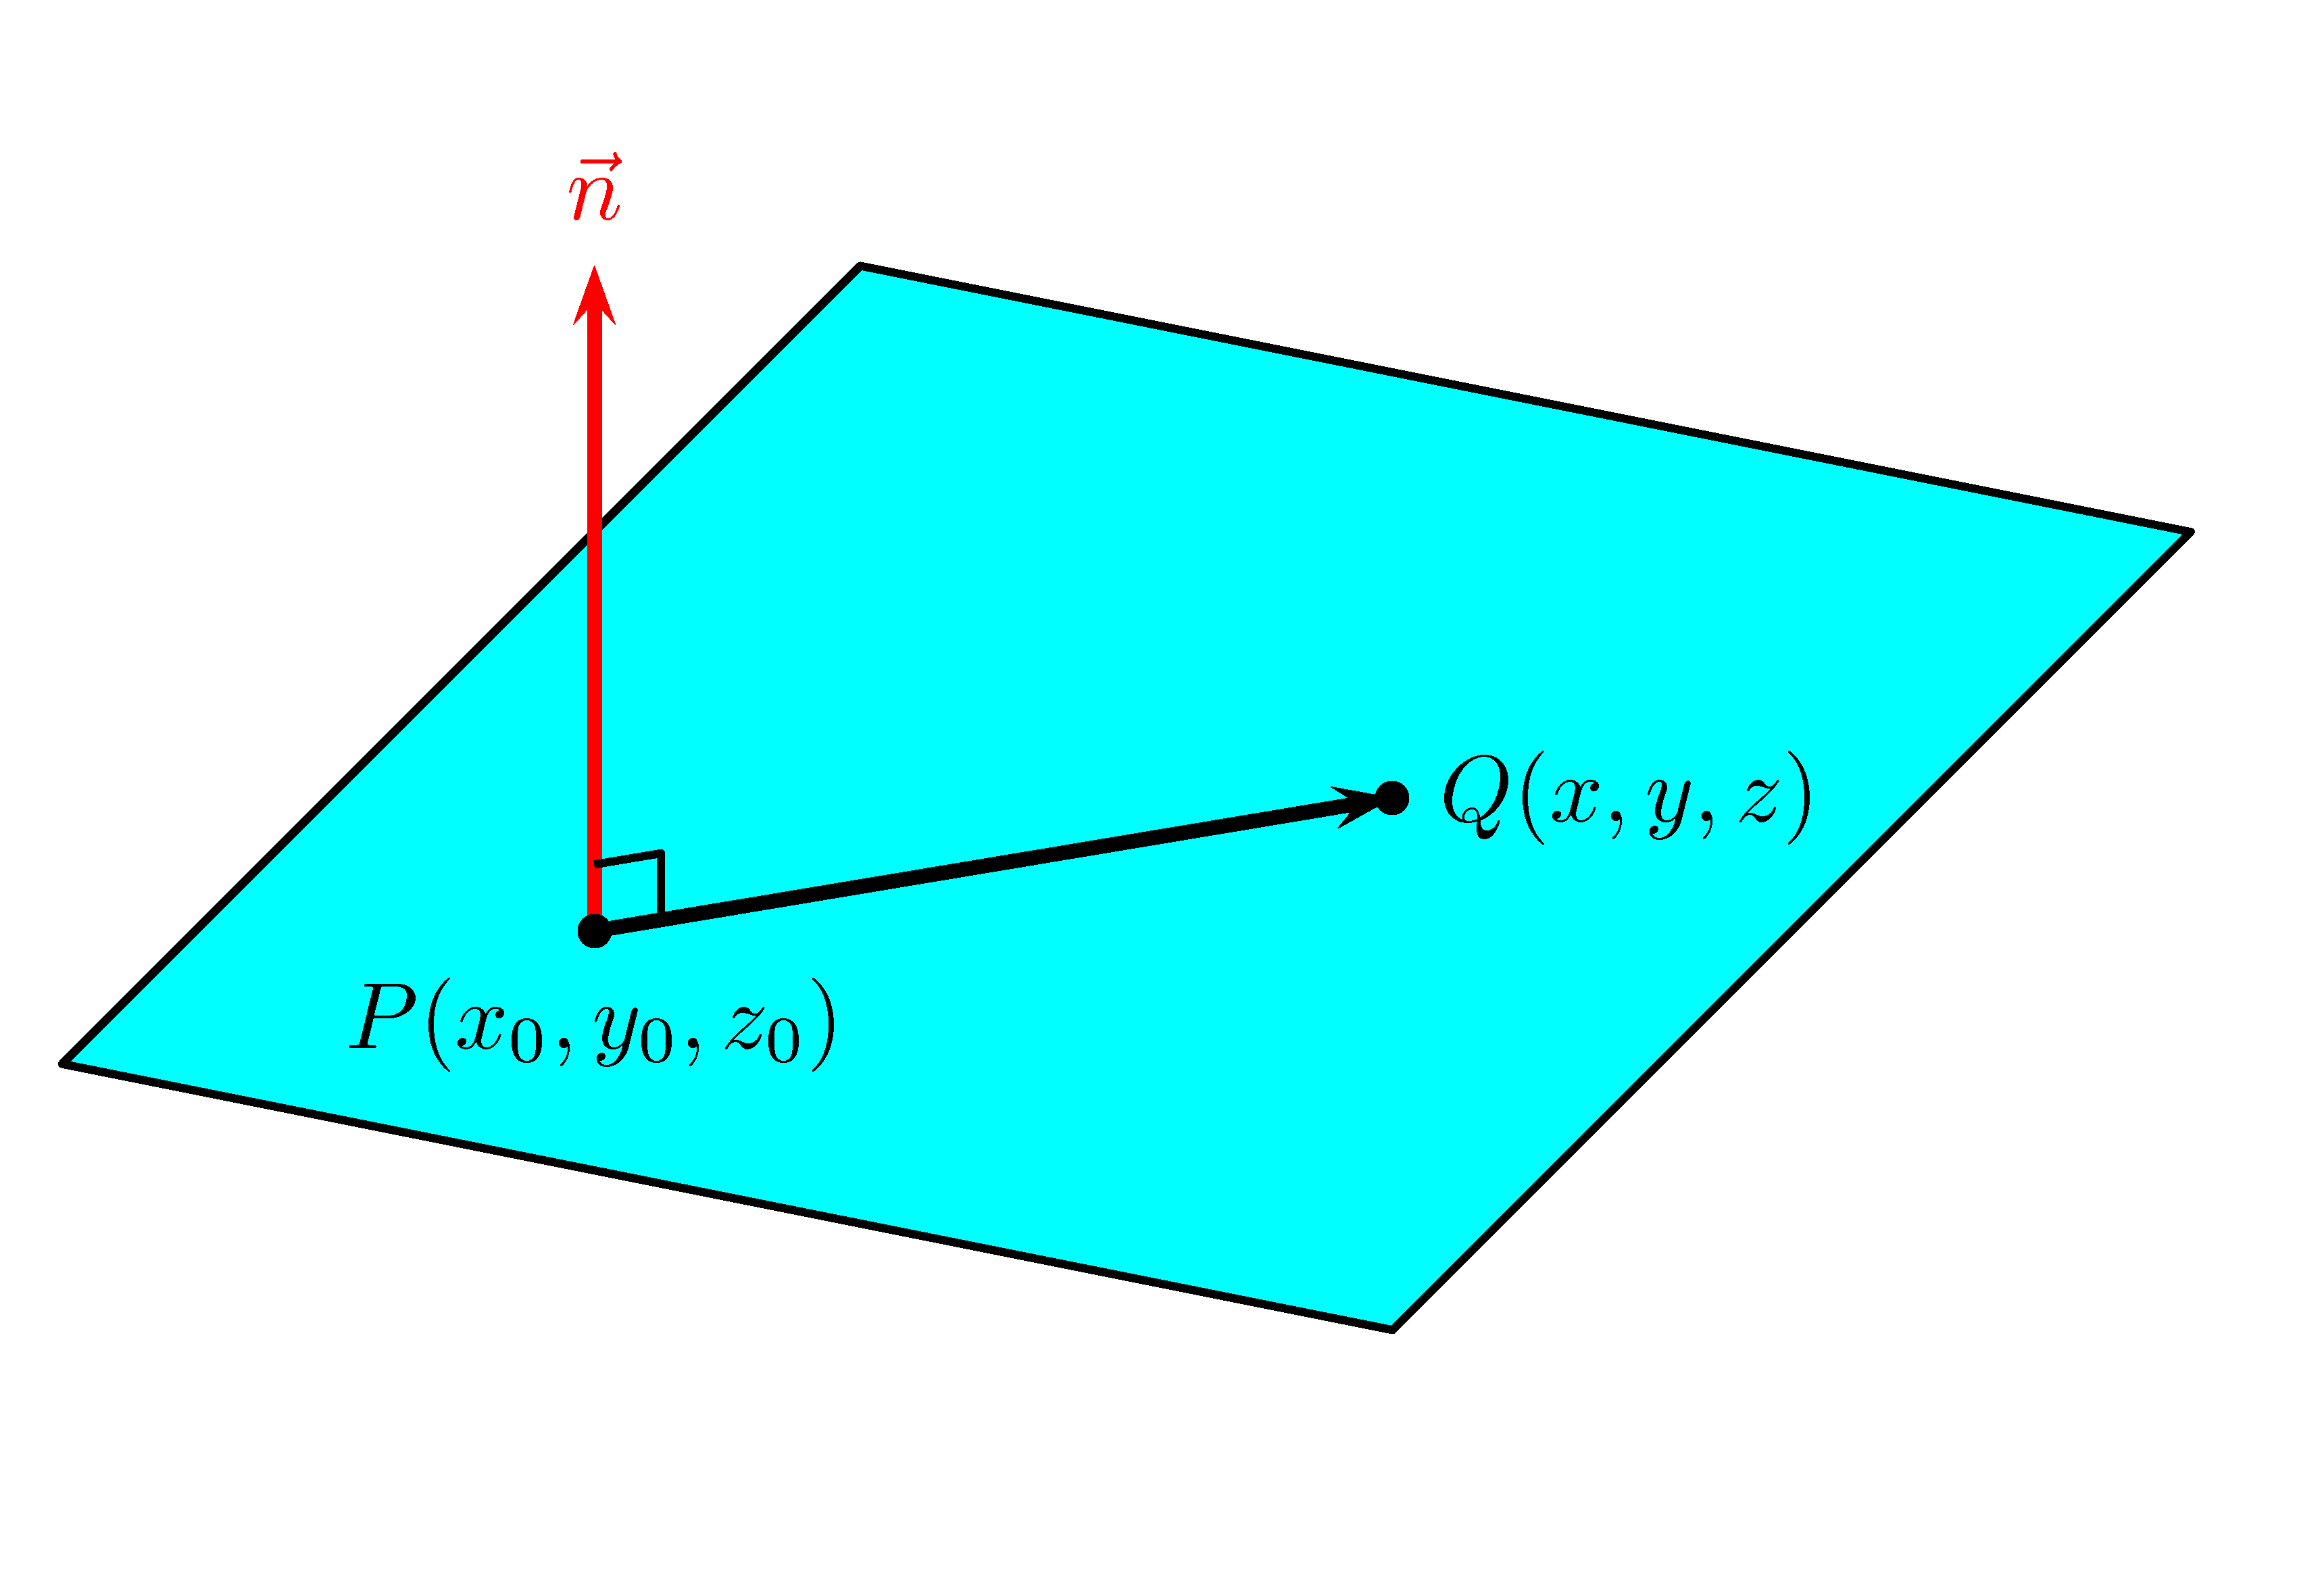
\includegraphics[width=0.75\linewidth]{resources/images/latex/eqcartesienneplan} 

}

\caption{Représentation d'un plan avec un de ses vecteur normal.}\label{fig:eq-cartesienne-plan}
\end{figure}

Puisque le vecteur normal \(\overrightarrow{n}\) est perpendiculaire à
tous les vecteurs se trouvant sur le plan, il est en particulier
perpendiculaire au vecteur \(\overrightarrow{PQ}\). Si nous définissons
le vecteur \(\overrightarrow{p} = \overrightarrow{OP}\) et le vecteur
\(\overrightarrow{x}=\overrightarrow{OQ}\), nous avons que:
\begin{align*}
\overrightarrow{n} \cdot (\overrightarrow{x} - \overrightarrow{p}) &= 0 \quad \text{car $\overrightarrow{n} \perp (\overrightarrow{x} - \overrightarrow{p})$}
\end{align*} Nous avons donc:

\BeginKnitrBlock{definition}[L'équation cartésienne d'un plan]
\protect\hypertarget{def:unnamed-chunk-170}{}{\label{def:unnamed-chunk-170}
\iffalse (L'équation cartésienne d'un plan) \fi{} }Soit un plan \(\pi\).
Soit un vecteur normal à ce plan \(\overrightarrow{n}=[a,b,c]\) et un
point de ce plan \(P(x_0,y_0,z_0)\) connu. L'équation normale du plan
est donnée par: \begin{align*}
\overrightarrow{n} \cdot (\overrightarrow{x} - \overrightarrow{p}) &= 0 \\
[a,b,c] \cdot [x-x_0,y-y_0,z-z_0] &= 0 \\
a(x-x_0)+b(y-y_0)+c(z-z_0) &= 0
\end{align*}
\EndKnitrBlock{definition}

Nous sommes maintenant prêts à trouver l'équation du plan tangent à une
surface. Pour simplifier la démonstration, nous allons modifier
l'équation cartésienne d'un plan.

\begin{align*}
a(x-x_0)+b(y-y_0)+c(z-z_0) &= 0 \\
c(z-z_0)  &= -a(x-x_0)-b(y-y_0) \\
z-z_0 &= \frac{-a}{c}(x-x_0)+\frac{-b}{c}(y-y_0) \\
&= A(x-x_0)+B(y-y_0)
\end{align*}

en posant \(A=-\frac{a}{c}\) et \(B=-\frac{b}{c}\).

Pour trouver les constantes \(A\) et \(B\), nous allons nous placer dans
les plans \(y=y_0\) et \(x=x_0\). Tout d'abord, plaçons-nous dans le
plan \(y=y_0\). Nous avons donc:

\begin{align*}
z-z_0 &= A(x-x_0)+B(y_0-y_0) \\
z-z_0 &= A(x-x_0) \\
z &= Ax +(z_0-Ax_0)
\end{align*}

L'équation précédente correspond à celle de la droite tangente à la
courbe définie par \(z=f(x,y_0)\). La pente de cette droite correspond à
la dérivée partielle de la fonction \(f\) par rapport à \(x\), évaluée
en \((x_0,y_0)\), c'est-à-dire
\(A=\left.\dfrac{\partial f}{\partial x}\right|_{(x_0,y_0)}\).

D'une manière similaire, nous montrons que
\(B=\left.\dfrac{\partial f}{\partial y}\right|_{(x_0,y_0)}\).

L'équation du plan tangent est don donnée par:

\[ z = z_0 + \left.\dfrac{\partial f}{\partial x}\right|_{(x_0,y_0)}\cdot (x-x_0)+\left.\dfrac{\partial f}{\partial y}\right|_{(x_0,y_0)}\cdot (y-y_0) \]

\BeginKnitrBlock{example}
\protect\hypertarget{exm:unnamed-chunk-171}{}{\label{exm:unnamed-chunk-171}
}Trouvez l'équation du plan tangent à la surface \(f(x,y)=9-x^2-y^2\) au
point \((1,1)\).
\EndKnitrBlock{example}
\vspace*{8cm}

\BeginKnitrBlock{example}
\protect\hypertarget{exm:unnamed-chunk-172}{}{\label{exm:unnamed-chunk-172}
}Trouvez l'équation du plan tangent à la surface \(f(x,y)=\sin(xy)\) au
point \(\left(\frac{\pi}{3},-1 \right)\).
\EndKnitrBlock{example}
\vspace*{8cm}

\BeginKnitrBlock{example}
\protect\hypertarget{exm:unnamed-chunk-173}{}{\label{exm:unnamed-chunk-173}
}Trouvez le plan tangent horizontal à la surface
\(f(x,y)=x^2-4xy-2y^2+12x-12y-1\)
\EndKnitrBlock{example}
\vspace*{8cm}

\BeginKnitrBlock{example}
\protect\hypertarget{exm:unnamed-chunk-174}{}{\label{exm:unnamed-chunk-174}
}Trouvez l'équation du plan tangent à la surface
\(f(x,y)=\dfrac{x-y}{x+y}\) au point \((1,1)\).
\EndKnitrBlock{example}
\vspace*{8cm}

\BeginKnitrBlock{remark}
\iffalse{} {Remarque. } \fi{}Le plan tangent est l'analogue du polynôme
de Taylor de degré 1 pour les fonctions de deux variables.
\EndKnitrBlock{remark}

\hypertarget{les-fonctions-differentiables}{%
\section{Les fonctions
différentiables}\label{les-fonctions-differentiables}}

\hypertarget{les-differentielles}{%
\subsection{Les différentielles}\label{les-differentielles}}

\hypertarget{le-calcul-dincertitude}{%
\subsection{Le calcul d'incertitude}\label{le-calcul-dincertitude}}

\BeginKnitrBlock{definition}[L'erreur absolue et l'erreur relative]
\protect\hypertarget{def:unnamed-chunk-176}{}{\label{def:unnamed-chunk-176}
\iffalse (L'erreur absolue et l'erreur relative) \fi{} }Soit \(a\) une
donnée que nous mesurons. Nous notons \(\Delta a\) l'erreur absolue de
la mesure \(a\), c'est-à-dire l'incertitude associée à la prise de
mesure de \(a\). Nous notons \(\dfrac{\Delta a}{a}\) l'erreur relative
de \(a\).
\EndKnitrBlock{definition}

Nous allons maintenant retrouver certaines règles de calcul
d'incertitude à l'aide de la différentielle totale d'une fonction.

Soit une fonction \(f(x_1,x_2,\ldots,x_n)\) une donnée dépendant de
\(n\) mesures notées \(x_1\), \(x_2\), \ldots{}, \(x_n\). D'après les
notions de différentielle, nous avons:

\[ df = \dfrac{\partial f}{\partial x_1} dx_1 + \ldots + \dfrac{\partial f}{\partial x_n} dx_n \]
Nous sommes maintenant en mesure de calculer une valeur maximale pour
\(df\):

\[ |df| \leq \left|\dfrac{\partial f}{\partial x_1}\right| |dx_1| + \ldots + \left|\dfrac{\partial f}{\partial x_n}\right| |dx_n| \]

En notant les incertitudes \(\Delta x = |dx|\) pour toutes les mesures,
nous obtenons la relation suivante en prenant la valeur maximale de
l'incertitude :

\[ \Delta f = \left|\dfrac{\partial f}{\partial x_1}\right| \Delta x_1 + \ldots + \left|\dfrac{\partial f}{\partial x_n}\right| \Delta x_n \]

\hypertarget{laddition-ou-la-soustraction-de-deux-mesures.}{%
\subsubsection{L'addition ou la soustraction de deux
mesures.}\label{laddition-ou-la-soustraction-de-deux-mesures.}}

Soit \(f(x_1,x_2)=x_1\pm x_2\). Nous avons: \begin{align*}
\Delta f &= \left| \dfrac{\partial f}{\partial x_1} \right| \Delta x_1
+ \left| \dfrac{\partial f}{\partial x_2} \right| \Delta x_2 \\
&= \Delta x_1 \pm \Delta x_2
\end{align*} Ceci implique que lors de l'addition ou de la soustraction
de deux mesures, les erreurs absolues sont additionnées.

\hypertarget{le-produit-dune-mesure-par-une-constante}{%
\subsubsection{Le produit d'une mesure par une
constante}\label{le-produit-dune-mesure-par-une-constante}}

Soit \(f(x_1)=kx_1\) où \(k\) est une constante. Nous avons:
\begin{align*}
\Delta f &= \left| \dfrac{\partial f}{\partial x_1} \right| \Delta x_1 \\
&= |k| \Delta x_1
\end{align*} Ceci implique que lors du produit d'une mesure par une
constante, l'erreur absolue de la mesure est multipliée par la valeur
absolue de la constante.

\hypertarget{le-produit-de-deux-mesures}{%
\subsubsection{Le produit de deux
mesures}\label{le-produit-de-deux-mesures}}

Soit \(f(x_1,x_2)=x_1 \cdot x_2\). Nous avons: \begin{align*}
\Delta f &= \left| \dfrac{\partial f}{\partial x_1} \right| \Delta x_1
+ \left| \dfrac{\partial f}{\partial x_2} \right| \Delta x_2 \\
&= |x_2| \Delta x_1 + |x_1| \Delta x_2 \\
\dfrac{\Delta f}{f} &= \dfrac{|x_2|}{x_1\cdot x_2}\Delta x_1 + \dfrac{|x_1|}{x_1\cdot x_2}\Delta x_2 \\
&= \dfrac{\Delta x_1}{x_1} + \dfrac{\Delta x_2}{x_2}
\end{align*} Ceci implique que lors du produit de deux mesures, les
erreurs relatives sont additionnées.

\hypertarget{le-quotient-de-deux-mesures}{%
\subsubsection{Le quotient de deux
mesures}\label{le-quotient-de-deux-mesures}}

Soit \(f(x_1,x_2)=\dfrac{x_1}{x_2}\). Nous avons: \begin{align*}
\Delta f &= \left| \dfrac{\partial f}{\partial x_1} \right| \Delta x_1
+ \left| \dfrac{\partial f}{\partial x_2} \right| \Delta x_2 \\
&= \left| \dfrac{1}{x_2} \right| \Delta x_1 + \left| \dfrac{-x_1}{x_2^2} \right| \Delta x_2 \\
\dfrac{\Delta f}{f} &= \left| \dfrac{1}{x_2}\dfrac{x_2}{x_1} \right| \Delta x_1 + \left| \dfrac{-x_1}{x_2^2}\dfrac{x_2}{x_1} \right| \Delta x_2 \\
&= \dfrac{\Delta x_1}{x_1} + \dfrac{\Delta x_2}{x_2}
\end{align*} Ceci implique que lors du quotient de deux mesures, les
erreurs relatives sont additionnées.

\hypertarget{la-puissance-dune-mesure}{%
\subsubsection{La puissance d'une
mesure}\label{la-puissance-dune-mesure}}

Soit \(f(x_1)=x_1^n\) où \(n\in\mathbb{R}\). Nous avons: \begin{align*}
\Delta f &= \left| \dfrac{\partial f}{\partial x_1} \right| \Delta x_1 \\
&= |nx_1^{n-1}| \Delta x_1 \\
\dfrac{\Delta f}{f} &= \left| \dfrac{nx_1^{n-1}}{x_1^n} \right| \Delta x_1 \\
&= |n| \dfrac{\Delta x_1}{x_1}
\end{align*} Ceci implique que lors du calcul de la puissance d'une
mesure, nous multiplions l'erreur relative par la valeur absolue de la
puissance \(n\).

\BeginKnitrBlock{example}
\protect\hypertarget{exm:unnamed-chunk-177}{}{\label{exm:unnamed-chunk-177}
}Pour mesurer le volume d'un cylindre, nous mesurons sa hauteur et son
rayon. Nous obtenons \(h=15\ \text{cm}\pm 0,1\ \text{cm}\) et
\(h=5\ \text{cm}\pm 0,1\ \text{cm}\). Trouvez l'erreur absolue et
l'erreur relative sur le volume du cylindre.
\EndKnitrBlock{example}
\vspace*{8cm}

\BeginKnitrBlock{example}
\protect\hypertarget{exm:unnamed-chunk-178}{}{\label{exm:unnamed-chunk-178}
}La période d'oscillation \(T\) d'un pendule simple dépend de la
longueur du pendule \(l\), \(T=2\pi\sqrt{\dfrac{l}{g}}\). En mesurant la
période du pendule et sa longueur (deux mesures), nous pouvons obtenir
la valeur de la constante gravitationnelle \(g=\dfrac{4\pi^2 l}{T^2}\).
Trouvez l'erreur absolue et l'erreur relative sur la mesure de \(g\), en
fonction des incertitudes sur \(T\) et \(l\).
\EndKnitrBlock{example}
\vspace*{8cm}

\hypertarget{la-regle-de-derivation-en-chaine-et-la-derivation-implicite}{%
\section{La règle de dérivation en chaîne et la dérivation
implicite}\label{la-regle-de-derivation-en-chaine-et-la-derivation-implicite}}

Nous savons que si \(y=f(x)\) et \(x=x(t)\), alors la dérivée de la
composition des fonctions \(f\circ x\) est:

\[ \dfrac{dy}{dt} = \dfrac{df}{dx}\dfrac{dx}{dt} \]

C'est ce que nous nommons la \textbf{règle de dérivation en chaîne}.
Nous voulons maintenant introduire une règle similaire pour les
fonctions de plusieurs variables. Débutons par étudier la règle pour les
fonctions de deux variables. La généralisation pour les fonctions de
trois variables ou plus se fait de façon similaire.

\BeginKnitrBlock{theorem}[La règle de dérivation en chaîne pour les fonctions de deux variables]
\protect\hypertarget{thm:deriv-chaine-1}{}{\label{thm:deriv-chaine-1}
\iffalse (La règle de dérivation en chaîne pour les fonctions de deux
variables) \fi{} }Soit une fonction différentiable \(z=f(x,y)\) et soit
\(x=x(t)\) et \(y=y(t)\). Nous avons alors:

\[ \dfrac{dz}{dt} = \dfrac{\partial f}{\partial x}\dfrac{dx}{dt}+
  \dfrac{\partial f}{\partial y}\dfrac{dy}{dt} \]
\EndKnitrBlock{theorem}

\BeginKnitrBlock{remark}
\iffalse{} {Remarque. } \fi{}La dérivée \(\dfrac{dz}{dt}\) est une
dérivée habituelle et non partielle. En effet, la fonction \(z=f(x,y)\)
ne dépend que d'une seule variable, \(t\). Lorsqu'une fonction dépend
d'une seule variable, nous utilisons \(d\) et lorsqu'elle dépend de deux
variables ou plus, nous utilisons \(\partial\).
\EndKnitrBlock{remark}

La manière la plus simple de trouver une dérivée à l'aide du théorème
\ref{thm:deriv-chaine-1}, est de construire un schéma de dérivation. Si
nous dessinons le schéma de dérivaton de la fonction du théorème
\ref{thm:deriv-chaine-1}, nous obtenons l'image suivante.

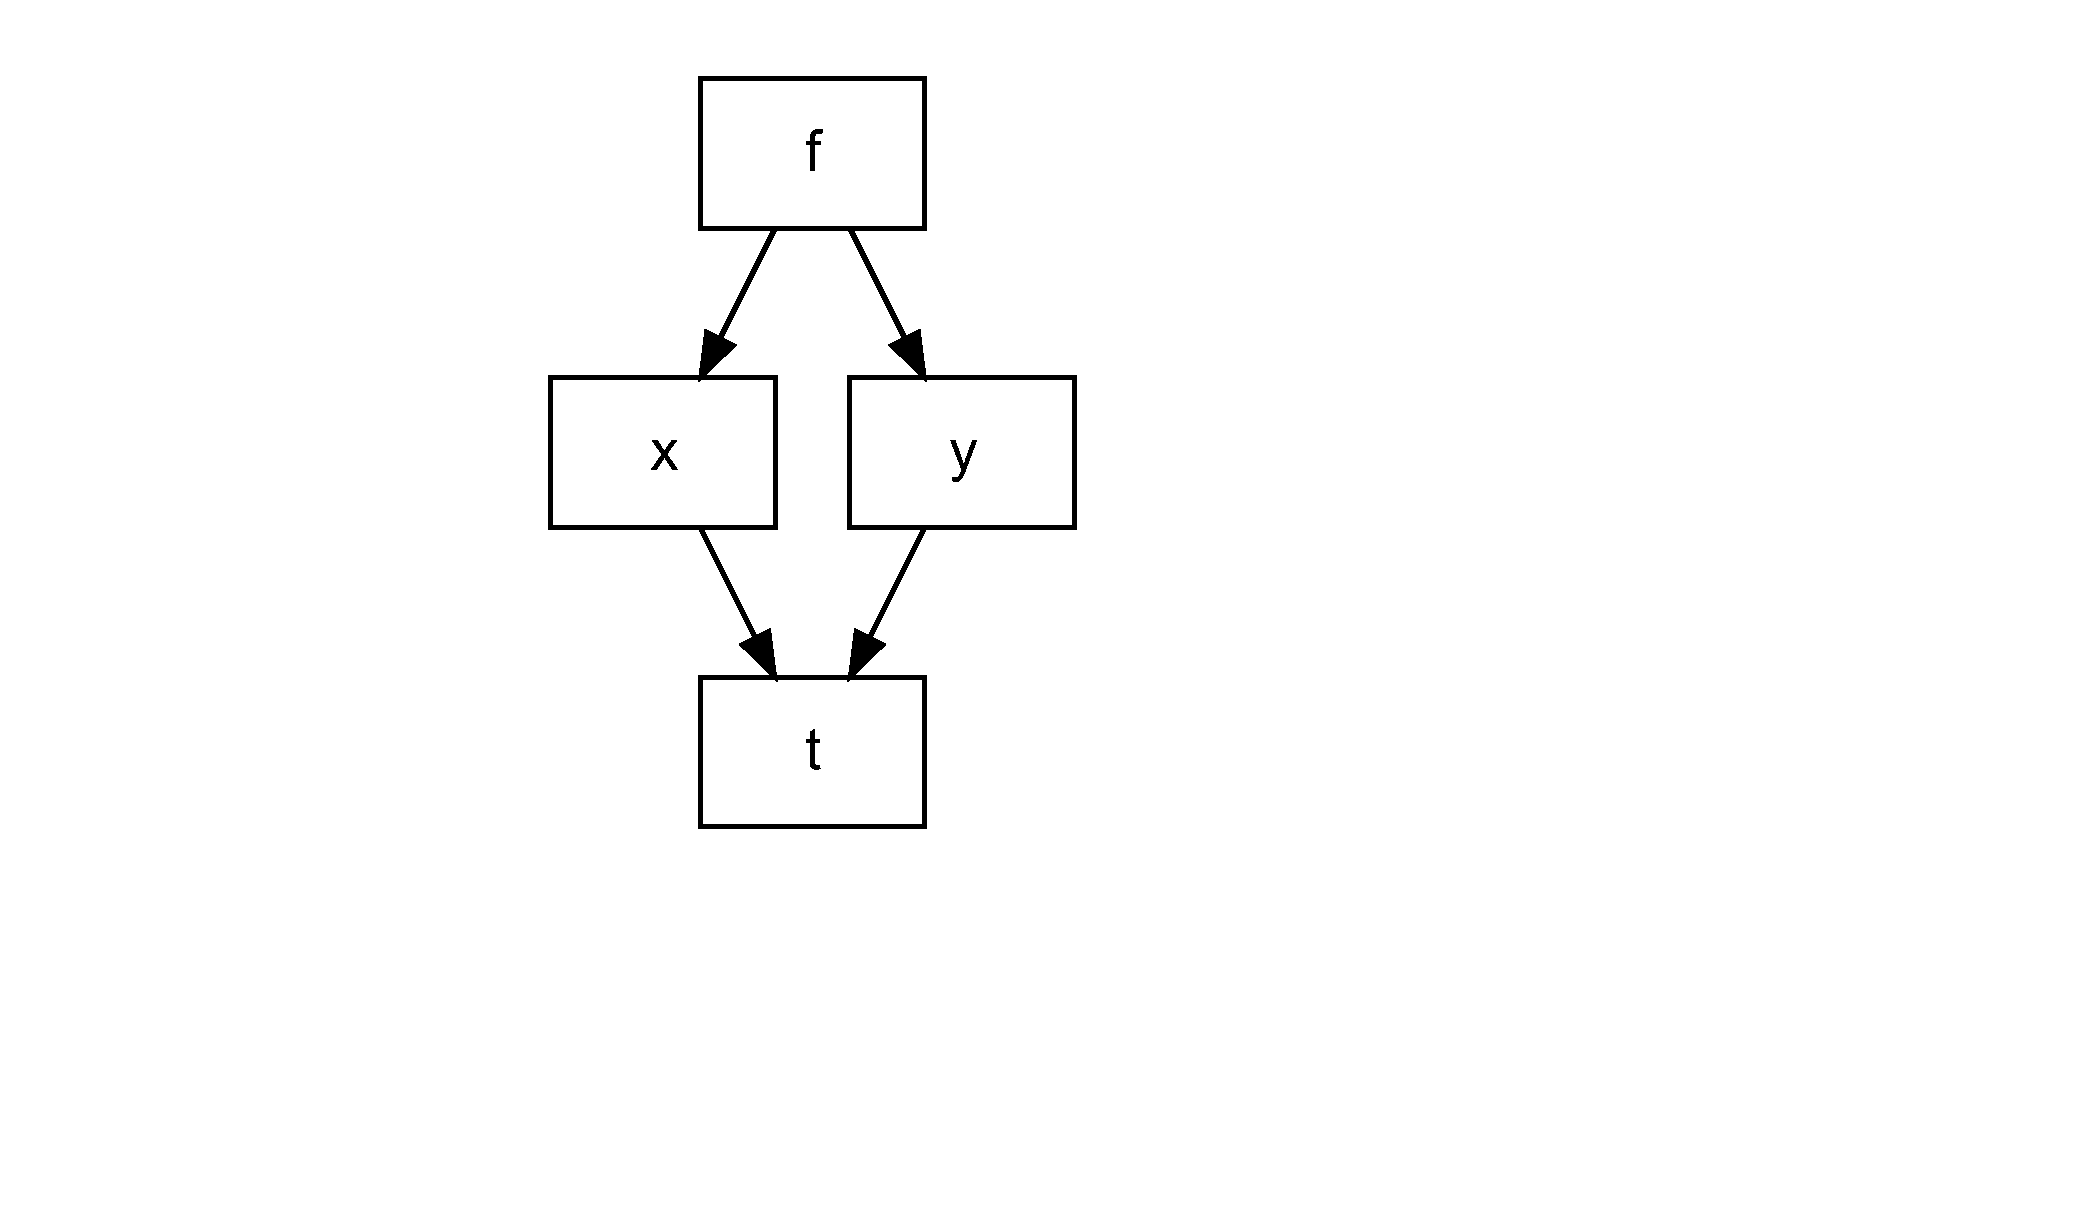
\includegraphics{calcul3_files/figure-latex/unnamed-chunk-180-1.pdf}

Pour dériver à la chaîne à l'aide de la figure précédente, nous partons
du haut de l'\emph{arbre} et nous parcourons toutes les \emph{branches}
qui se rendent jusqu'à la variable par rapport à laquelle nous dérivons,
en multipliant les dérivées. Nous additionnons toutes les
\emph{branches} pour obtenir la dérivée.

\BeginKnitrBlock{example}
\protect\hypertarget{exm:unnamed-chunk-181}{}{\label{exm:unnamed-chunk-181}
}Trouvez \(\dfrac{dz}{dt}\) si \(z=e^{xy^2}\), \(x=t\cos(t)\) et
\(y=t\sin(t)\).
\EndKnitrBlock{example}
\vspace*{8cm}

\BeginKnitrBlock{example}
\protect\hypertarget{exm:unnamed-chunk-182}{}{\label{exm:unnamed-chunk-182}
}Trouvez \(\dfrac{dz}{dt}\) si \(z=\sin(x^2y)\), \(x=2t^2\) et
\(y=2+\frac{1}{t}\).
\EndKnitrBlock{example}
\vspace*{8cm}

\BeginKnitrBlock{example}
\protect\hypertarget{exm:unnamed-chunk-183}{}{\label{exm:unnamed-chunk-183}
}Trouvez la dérivée de \(y=(\sin(x))^x\) de deux manières différentes.
\EndKnitrBlock{example}
\vspace*{10cm}

Nous voulons maintenant savoir ce qui se produit lorsque nous avons une
fonction \(z=f(x,y)\) différentiable, \(x=x(u,v)\) et \(y=y(u,v)\).

\BeginKnitrBlock{theorem}
\protect\hypertarget{thm:unnamed-chunk-184}{}{\label{thm:unnamed-chunk-184}
}Soit une fonction \(z=f(x,y)\) différentiable, \(x=x(u,v)\) et
\(y=y(u,v)\). Nous avons: \begin{align*}
\dfrac{\partial z}{\partial u} &= \dfrac{\partial f}{\partial x}\dfrac{\partial x}{\partial u} + \dfrac{\partial f}{\partial y}\dfrac{\partial y}{\partial u} \\
\dfrac{\partial z}{\partial v} &= \dfrac{\partial f}{\partial x}\dfrac{\partial x}{\partial v} + \dfrac{\partial f}{\partial y}\dfrac{\partial y}{\partial v}
\end{align*}
\EndKnitrBlock{theorem}

\BeginKnitrBlock{proof}
\iffalse{} {Preuve. } \fi{}Nous ne ferons pas la preuve exacte mais nous
allons dessiner le schéma de dérivation.
\EndKnitrBlock{proof}

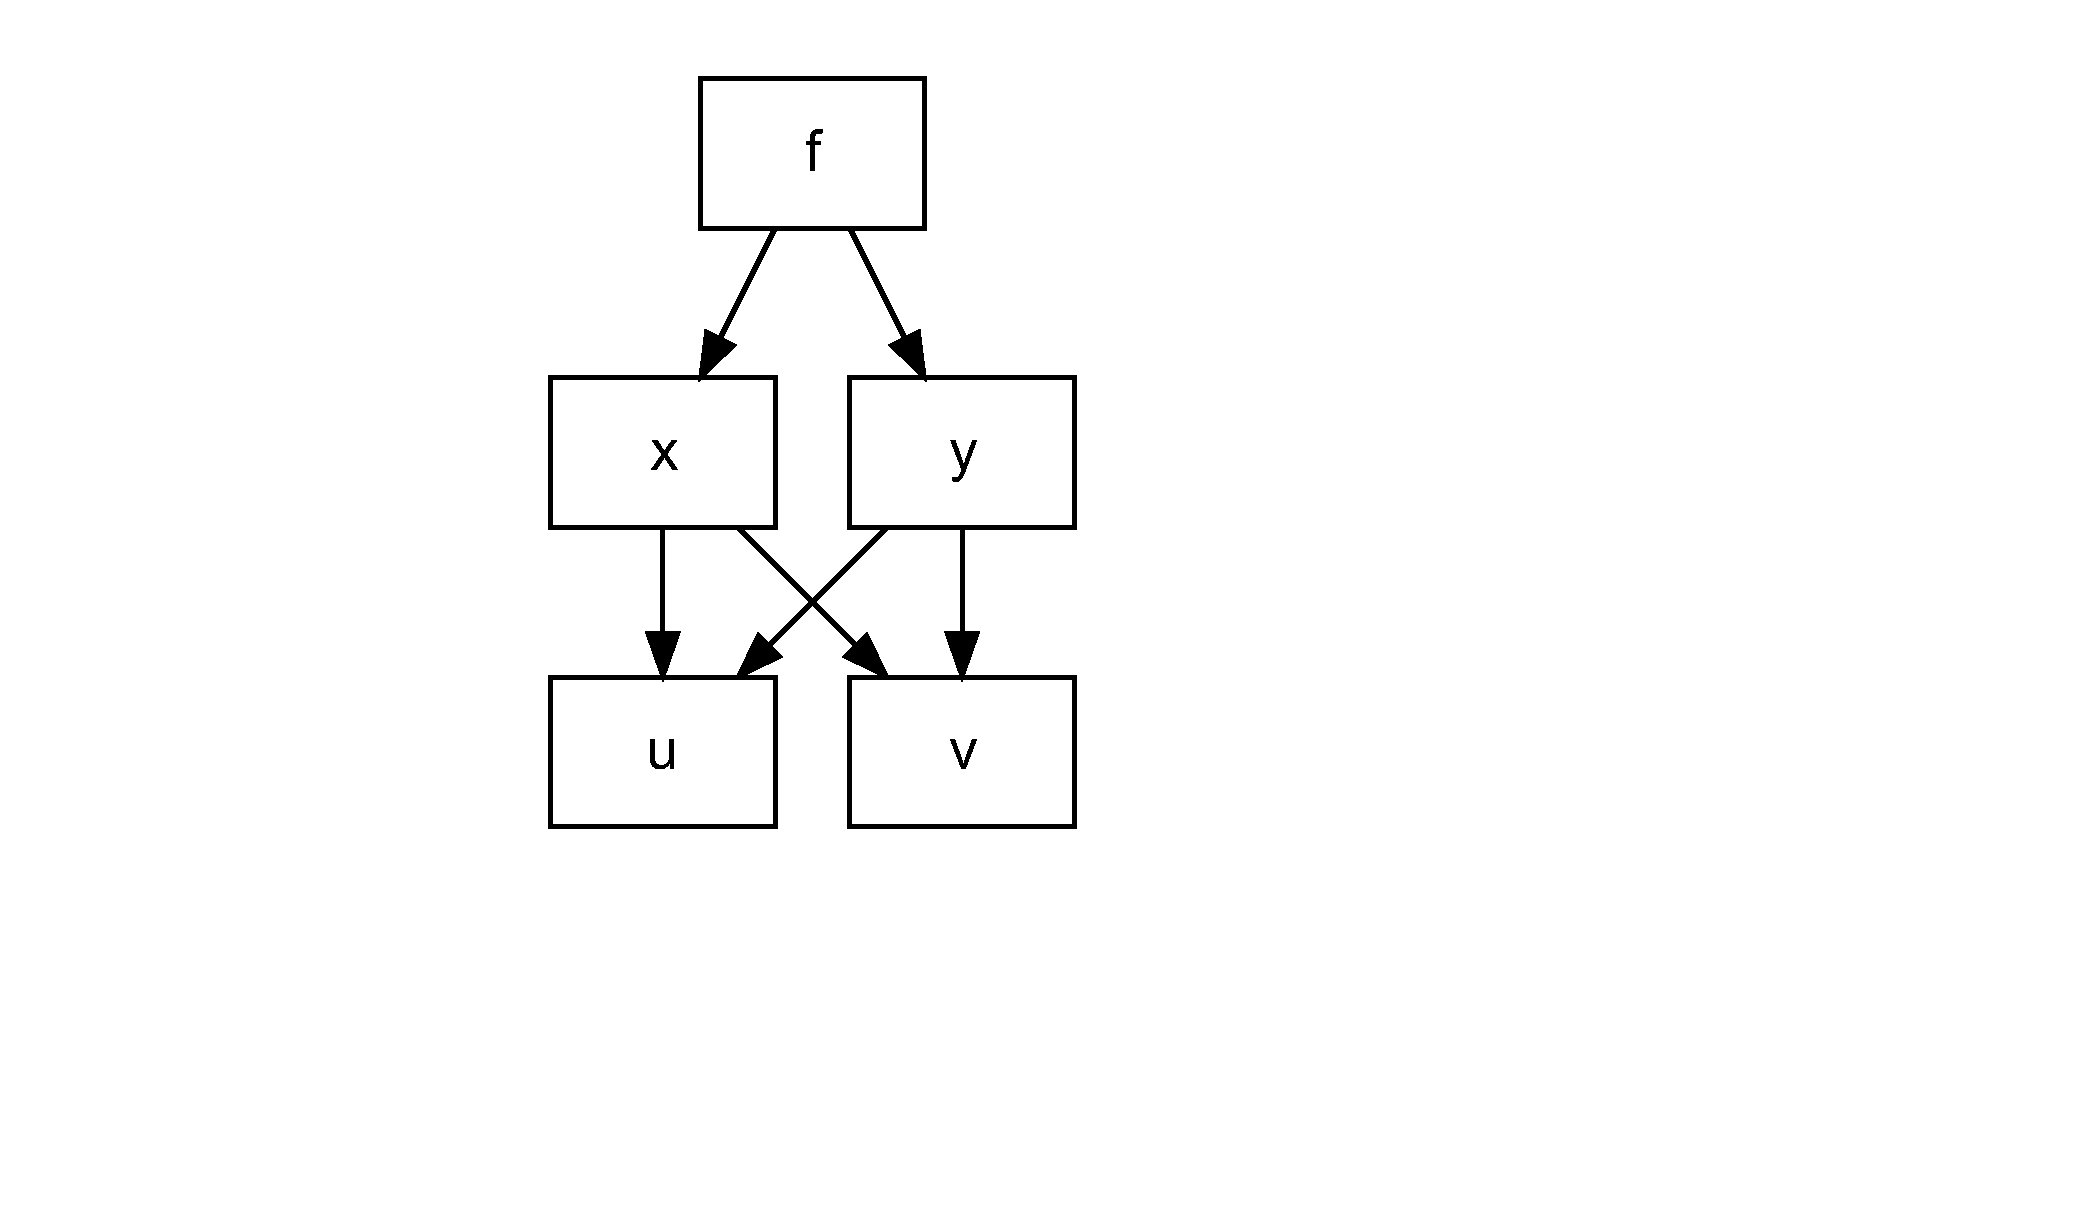
\includegraphics{calcul3_files/figure-latex/unnamed-chunk-186-1.pdf}
Remarquons que si nous suivons toutes les \emph{branches} de
l'\emph{arbre} en multipliant les dérivées et en additionnant les
branches, nous obtenons le résultat du théorème. ```

\BeginKnitrBlock{example}
\protect\hypertarget{exm:unnamed-chunk-187}{}{\label{exm:unnamed-chunk-187}
}Déterminez \(\dfrac{\partial z}{\partial u}\) et
\(\dfrac{\partial z}{\partial v}\) si \(z=x^2+y^2\), \(x=uv\) et
\(y=\dfrac{u}{v}\).
\EndKnitrBlock{example}
\vspace*{8cm}

\BeginKnitrBlock{example}
\protect\hypertarget{exm:unnamed-chunk-188}{}{\label{exm:unnamed-chunk-188}
}Déterminez \(\dfrac{\partial z}{\partial u}\) et
\(\dfrac{\partial z}{\partial v}\) si \(z=\sqrt{x^2+y^2}\), \(x=e^{uv}\)
et \(y=1+u^2\cos(v)\).
\EndKnitrBlock{example}
\vspace*{8cm}

\hypertarget{les-derivees-de-surfaces-implicites}{%
\subsection{Les dérivées de surfaces
implicites}\label{les-derivees-de-surfaces-implicites}}

Certaines surfaces sont définies de façon implicites et il est parfois
plus simple de les dériver implicitement plutôt que de tenter de les
dériver de façon explicite. De plus, certaines surfaces ne peuvent pas
être exprimées de façon explicite.

Pour dériver de façon implicite, il faut garder en mémoire que si la
fonction possède \(n\) variables, alors une des \(n\) variables dépend
des \(n-1\) autres.

\BeginKnitrBlock{example}
\protect\hypertarget{exm:deriv-implicite-sphere}{}{\label{exm:deriv-implicite-sphere}
}Trouvez \(\dfrac{\partial z}{\partial x}\) et
\(\dfrac{\partial z}{\partial y}\) si \(x^2+y^2+z^2=R^2\), où \(R\) est
une constante.
\EndKnitrBlock{example}
\vspace*{8cm}

\BeginKnitrBlock{example}
\protect\hypertarget{exm:unnamed-chunk-189}{}{\label{exm:unnamed-chunk-189}
}Utilisez les dérivées trouvées à l'exemple
\ref(exm:deriv-implicite-sphere) pour trouver l'équation du plan tangent
à la sphère \(x^2+y^2+z^2=3\) au point (1,1,1).
\EndKnitrBlock{example}
\vspace*{8cm}

\BeginKnitrBlock{example}
\protect\hypertarget{exm:unnamed-chunk-190}{}{\label{exm:unnamed-chunk-190}
}Trouvez l'équation du plan tangent à la surface
\(\dfrac{x^2}{a^2}+\dfrac{y^2}{b^2}+\dfrac{z^2}{c^2}=1\) au point
\(\left( \frac{a}{\sqrt{3}},\frac{b}{\sqrt{3}},\frac{c}{\sqrt{3}} \right)\).
\EndKnitrBlock{example}
\vspace*{8cm}

\BeginKnitrBlock{example}
\protect\hypertarget{exm:unnamed-chunk-191}{}{\label{exm:unnamed-chunk-191}
}Utilisez le changement de variables \(r=x+ct\), \(s=x-ct\) et
\(w(r,s)=u(x,t)\) pour transformer l'équation suivante:
\[ \dfrac{\partial^2 u}{\partial t^2} = c^2\dfrac{\partial^2 u}{\partial x^2} \]
\EndKnitrBlock{example}
\vspace*{10cm}

\hypertarget{la-derivee-directionnelle}{%
\section{La dérivée directionnelle}\label{la-derivee-directionnelle}}

Nous avons jusqu'à maintenant étudié les dérivées partielles d'une
fonction par rapport aux variables \(x\) et \(y\). Celles-ci
correspondent respectivement au taux de variation de la fonction dans la
direction de l'axe des \(x\) et de l'axe des \(y\). Nous aimerions
maintenant trouver le taux de variation dans une autre direction. Nous
utiliserons pour ce faire la dérivée directionnelle.

\BeginKnitrBlock{definition}[La dérivée directionnelle]
\protect\hypertarget{def:deriv-directionnelle}{}{\label{def:deriv-directionnelle}
\iffalse (La dérivée directionnelle) \fi{} }Soit une fonction
\(z=f(x,y)\) une fonction différentiable et
\(\overrightarrow{u}=[u_1,u_2]\), un vecteur unitaire (c'est-à-dire un
vecteur dont la norme est égale à \(1\)). Nous disons que la dérivée de
\(f\) dans la direction \(\overrightarrow{u}\), notée
\(D_{\overrightarrow{u}}f\),est donnée par:
\[ D_{\overrightarrow{u}}f = \lim_{h\to 0} \dfrac{f(x+hu_1,y+hu_2)-f(x,y)}{h} \]
si cette limite existe.
\EndKnitrBlock{definition}

Pour visualiser la dérivée directionnelle, nous vous invitons à utiliser
l'application GeoGebra de la section \ref{geogebra-derivfctvar}.
Celle-ci vous permet de changer la direction du vecteur unitaire et le
point auquel vous visualisez la dérivée directionnelle.

\BeginKnitrBlock{remark}
\iffalse{} {Remarque. } \fi{}Nous remarquons que si
\(\overrightarrow{u}=[1,0]=\overrightarrow{\imath}\), nous obtenons la
dérivée partielle par rapport à \(x\). D'une manière similaire, si
\(\overrightarrow{u}=[0,1]=\overrightarrow{\jmath}\), nous obtenons la
dérivée partielle par rapport à \(x\).
\EndKnitrBlock{remark}

L'utilisation de la définition \ref{def:deriv-directionnelle} pour
calculer des dérivées directionnelles n'est pas appropriée pour la
plupart des problèmes. Le théorème suivant nous permettra de calculer la
dérivée directionnelles plus simplement.

\BeginKnitrBlock{theorem}
\protect\hypertarget{thm:derivee-directionnelle}{}{\label{thm:derivee-directionnelle}
}Soit une fonction \(z=f(x,y)\) différentiable au point \((x_0,y_0)\) et
soit \(\overrightarrow{u}=[u_1,u_2]\) un vecteur unitaire. Nous avons:
\[ D_{\overrightarrow{u}}f(x_0,y_0) = f_x(x_0,y_0)u_1 + f_y(x_0,y_0)u_2 \]
\EndKnitrBlock{theorem}

\BeginKnitrBlock{proof}
\iffalse{} {Preuve. } \fi{}Posons \(g(h)=f(x+u_1h,y+u_2h)\). Nous avons:
\begin{align}
D_{\overrightarrow{u}}f(x_0,y_0) &= \lim_{h\to 0} \dfrac{f(x+hu_1,y+hu_2)-f(x,y)}{h} \notag\\
&= \lim_{h\to 0} \dfrac{g(h)-g(0)}{h} \notag\\
&= g'(0) \label{eq:deriv-directionnelle} \quad \text{par définition de $g'$}
\end{align} Posons manitenant \(x=x_0+u_1h\) et \(y=y_0+u_2h\). D'où
\(g(h)=f(x,y)\). Par la règle de dérivation en chaîne, nous avons
\(g'(h)=f_xu_1+f_yu_2\). Si nous évaluons cette expression en \(h=0\) ,
nous obtenons: \begin{align*}
g'(0) &= f_x(x_0,y_0)u_1+f_y(x_0,y_0)u_2 \\
&= D_{\overrightarrow{u}}f(x_0,y_0)
\end{align*} La dernière ligne est obtenue par l'équation
\eqref{eq:deriv-directionnelle}.
\EndKnitrBlock{proof}

\BeginKnitrBlock{example}
\protect\hypertarget{exm:unnamed-chunk-194}{}{\label{exm:unnamed-chunk-194}
}Déterminez le taux de variation de \(f(x,y)=\cos(xy)+y^2\) dans la
direction du vecteur \(\overrightarrow{u}=[1,1]\).
\EndKnitrBlock{example}
\vspace*{8cm}

\BeginKnitrBlock{example}
\protect\hypertarget{exm:unnamed-chunk-195}{}{\label{exm:unnamed-chunk-195}
}Trouvez la dérivée directionnelle de \(f(x,y)=y^4+2xy^3+x^2y^2\) en
\((0,1)\) dans les directions suivantes:

\begin{enumerate}
\def\labelenumi{\alph{enumi}.}
\tightlist
\item
  \(\overrightarrow{u} =[1,2]\)
\item
  \(\overrightarrow{u} =[-2,1]\)
\item
  \(\overrightarrow{u} =[1,1]\)
\end{enumerate}
\EndKnitrBlock{example}
\vspace*{10cm}

\hypertarget{le-vecteur-gradient}{%
\section{Le vecteur gradient}\label{le-vecteur-gradient}}

Nous allons maintenant définir une fonction vectorielle très utile, le
vecteur gradient.

\BeginKnitrBlock{definition}[Le vecteur gradient]
\protect\hypertarget{def:unnamed-chunk-196}{}{\label{def:unnamed-chunk-196}
\iffalse (Le vecteur gradient) \fi{} }Soit \(z=f(x,y)\) une fonction
différentiable. Le gradient de \(f\), noté \(\nabla f\), est donné par:
\[ \nabla f = \left[\dfrac{\partial f}{\partial x},\dfrac{\partial f}{\partial y}\right] \]
Nous notons le gradient de \(f\) des façons suivantes: \(\nabla f\),
\(\text{grad } f\) et \(\overrightarrow{\text{grad}} f\).

Le gradient d'une fonction est un vecteur.
\EndKnitrBlock{definition}

\BeginKnitrBlock{example}
\protect\hypertarget{exm:unnamed-chunk-197}{}{\label{exm:unnamed-chunk-197}
}Trouvez le gradient de la fonction \(f(x,y)=x^2+3xy^5-4y^4\).
\EndKnitrBlock{example}
\vspace*{4cm}

\BeginKnitrBlock{example}
\protect\hypertarget{exm:unnamed-chunk-198}{}{\label{exm:unnamed-chunk-198}
}Trouvez le gradient des fonctions suivantes:

\begin{enumerate}
\def\labelenumi{\alph{enumi}.}
\tightlist
\item
  \(f(x,y)=x^2-y^2\)
\item
  \(f(x,y)=\dfrac{x-y}{x+y}\)
\end{enumerate}
\EndKnitrBlock{example}
\vspace*{8cm}

Le vecteur gradient est très utile ccar celui-ci possède plusieurs
caractéristiques intéressantes.

\BeginKnitrBlock{theorem}
\protect\hypertarget{thm:unnamed-chunk-199}{}{\label{thm:unnamed-chunk-199}
}Soit \(f(x,y)\) une fonction différentiable et \(\overrightarrow{u}\)
un vecteur unitaire. Nous avons alors:
\[ D_{\overrightarrow{u}} f = \nabla f \cdot \overrightarrow{u} \]
\EndKnitrBlock{theorem}

\BeginKnitrBlock{proof}
\iffalse{} {Preuve. } \fi{}Nous avons: \begin{align*}
\nabla f \cdot \overrightarrow{u} &= \left[\dfrac{\partial f}{\partial x},\dfrac{\partial f}{\partial y}\right] \cdot [u_1,u_2] \\
&= \dfrac{\partial f}{\partial x}u_1 + \dfrac{\partial f}{\partial y}u_2 \\
&= D_{\overrightarrow{u}} f
\end{align*} La dernière ligne est obtenue par le théorème
\ref{thm:derivee-directionnelle}.
\EndKnitrBlock{proof}

\BeginKnitrBlock{theorem}
\protect\hypertarget{thm:unnamed-chunk-201}{}{\label{thm:unnamed-chunk-201}
}Le vecteur gradient d'une fonction \(f\) pointe dans la direction
d'accroissement maximal de celle-ci. De plus, le taux de variation dans
cette direction est donné par la norme du gradient.
\EndKnitrBlock{theorem}

\BeginKnitrBlock{proof}
\iffalse{} {Preuve. } \fi{}Soit un vecteur unitaire
\(\overrightarrow{u}\). La dérivée directionnelle de \(f\) dans la
direction de \(\overrightarrow{u}\) est donnée par
\(D_{\overrightarrow{u}} f = \nabla f \cdot \overrightarrow{u}\). Nous
voulons trouvez \(\overrightarrow{u}\) tel que cette dérivée est
maximale. Nous savons que: \begin{align*}
\nabla f \cdot \overrightarrow{u} &= ||\nabla f || \cdot ||\overrightarrow{u} || \cos(\theta) \\
&= ||\nabla f || \cos(\theta) \quad \text{car $\overrightarrow{u}$ est unitaire}
\end{align*} où \(\theta\) est l'angle entre \(\nabla f\) et
\(\overrightarrow{u}\). Le membre de droite est maximal si
\(\cos(\theta)=1\), c'est-à-dire lorsque \(\theta=0\). D'où la direction
maximale est celle donnée par le vecteur gradient.

De plus, dans cette direction, la dérivée directionnelle est
\(D_{\overrightarrow{u}} f=||\nabla f ||\).
\EndKnitrBlock{proof}

\BeginKnitrBlock{example}
\protect\hypertarget{exm:unnamed-chunk-203}{}{\label{exm:unnamed-chunk-203}
}Soit la fonction \(f(x,y)=xe^{-x^2-y^2}\). Déterminez la direction dans
laquelle se trouve l'accroissement maximal au point \((1,1)\) et le taux
de variation maximal.
\EndKnitrBlock{example}
\vspace*{5cm}

\BeginKnitrBlock{example}
\protect\hypertarget{exm:unnamed-chunk-204}{}{\label{exm:unnamed-chunk-204}
}Soit la fonction \(f(x,y)=(x+y^2)e^{-x}\). Déterminez la direction dans
laquelle se trouve l'accroissement maximal au point \((1,1)\) et le taux
de variation maximal.
\EndKnitrBlock{example}
\vspace*{5cm}

La dernière propriété que nous verrons concernant le vecteur gradient
met en relation celui-ci avec les courbes de niveau d'une fonction.

\BeginKnitrBlock{theorem}
\protect\hypertarget{thm:unnamed-chunk-205}{}{\label{thm:unnamed-chunk-205}
}Le vecteur gradient d'une fonction est perpendiculaire aux courbes de
niveaux de cette fonction.
\EndKnitrBlock{theorem}

\BeginKnitrBlock{proof}
\iffalse{} {Preuve. } \fi{}Soit un point \((x_0,y_0)\) du domaine de la
fonction \(f\). Soit \(\overrightarrow{u}\) un vecteur unitaire pointant
dans la direction de la courbe de niveau passant par le point
\((x_0,y_0)\). La figure \ref{fig:gradientcourbeniveaux} représente
cette situation.

À ce moment, nous avons \(D_{\overrightarrow{u}} f(x_0,y_0)=0\), car la
fonction ne varie pas le long d'une courbe de niveau. Nous pouvons
également écrire
\(D_{\overrightarrow{u}} f(x_0,y_0)=0=||\nabla f(x_0,y_0)||\cos(\theta)\),
où \(\theta\) est l'angle entre le vecteur gradient et
\(\overrightarrow{u}\). Puisque \(||\nabla f(x_0,y_0)||\) n'est pas
obligatoirement nul, nous avons que:
\[ \cos(\theta) = 0 \Longrightarrow \theta=\dfrac{\pi}{2} \] Ainsi, le
gradient est perpendiculaire aux courbes de niveaux.
\EndKnitrBlock{proof}

\begin{figure}

{\centering 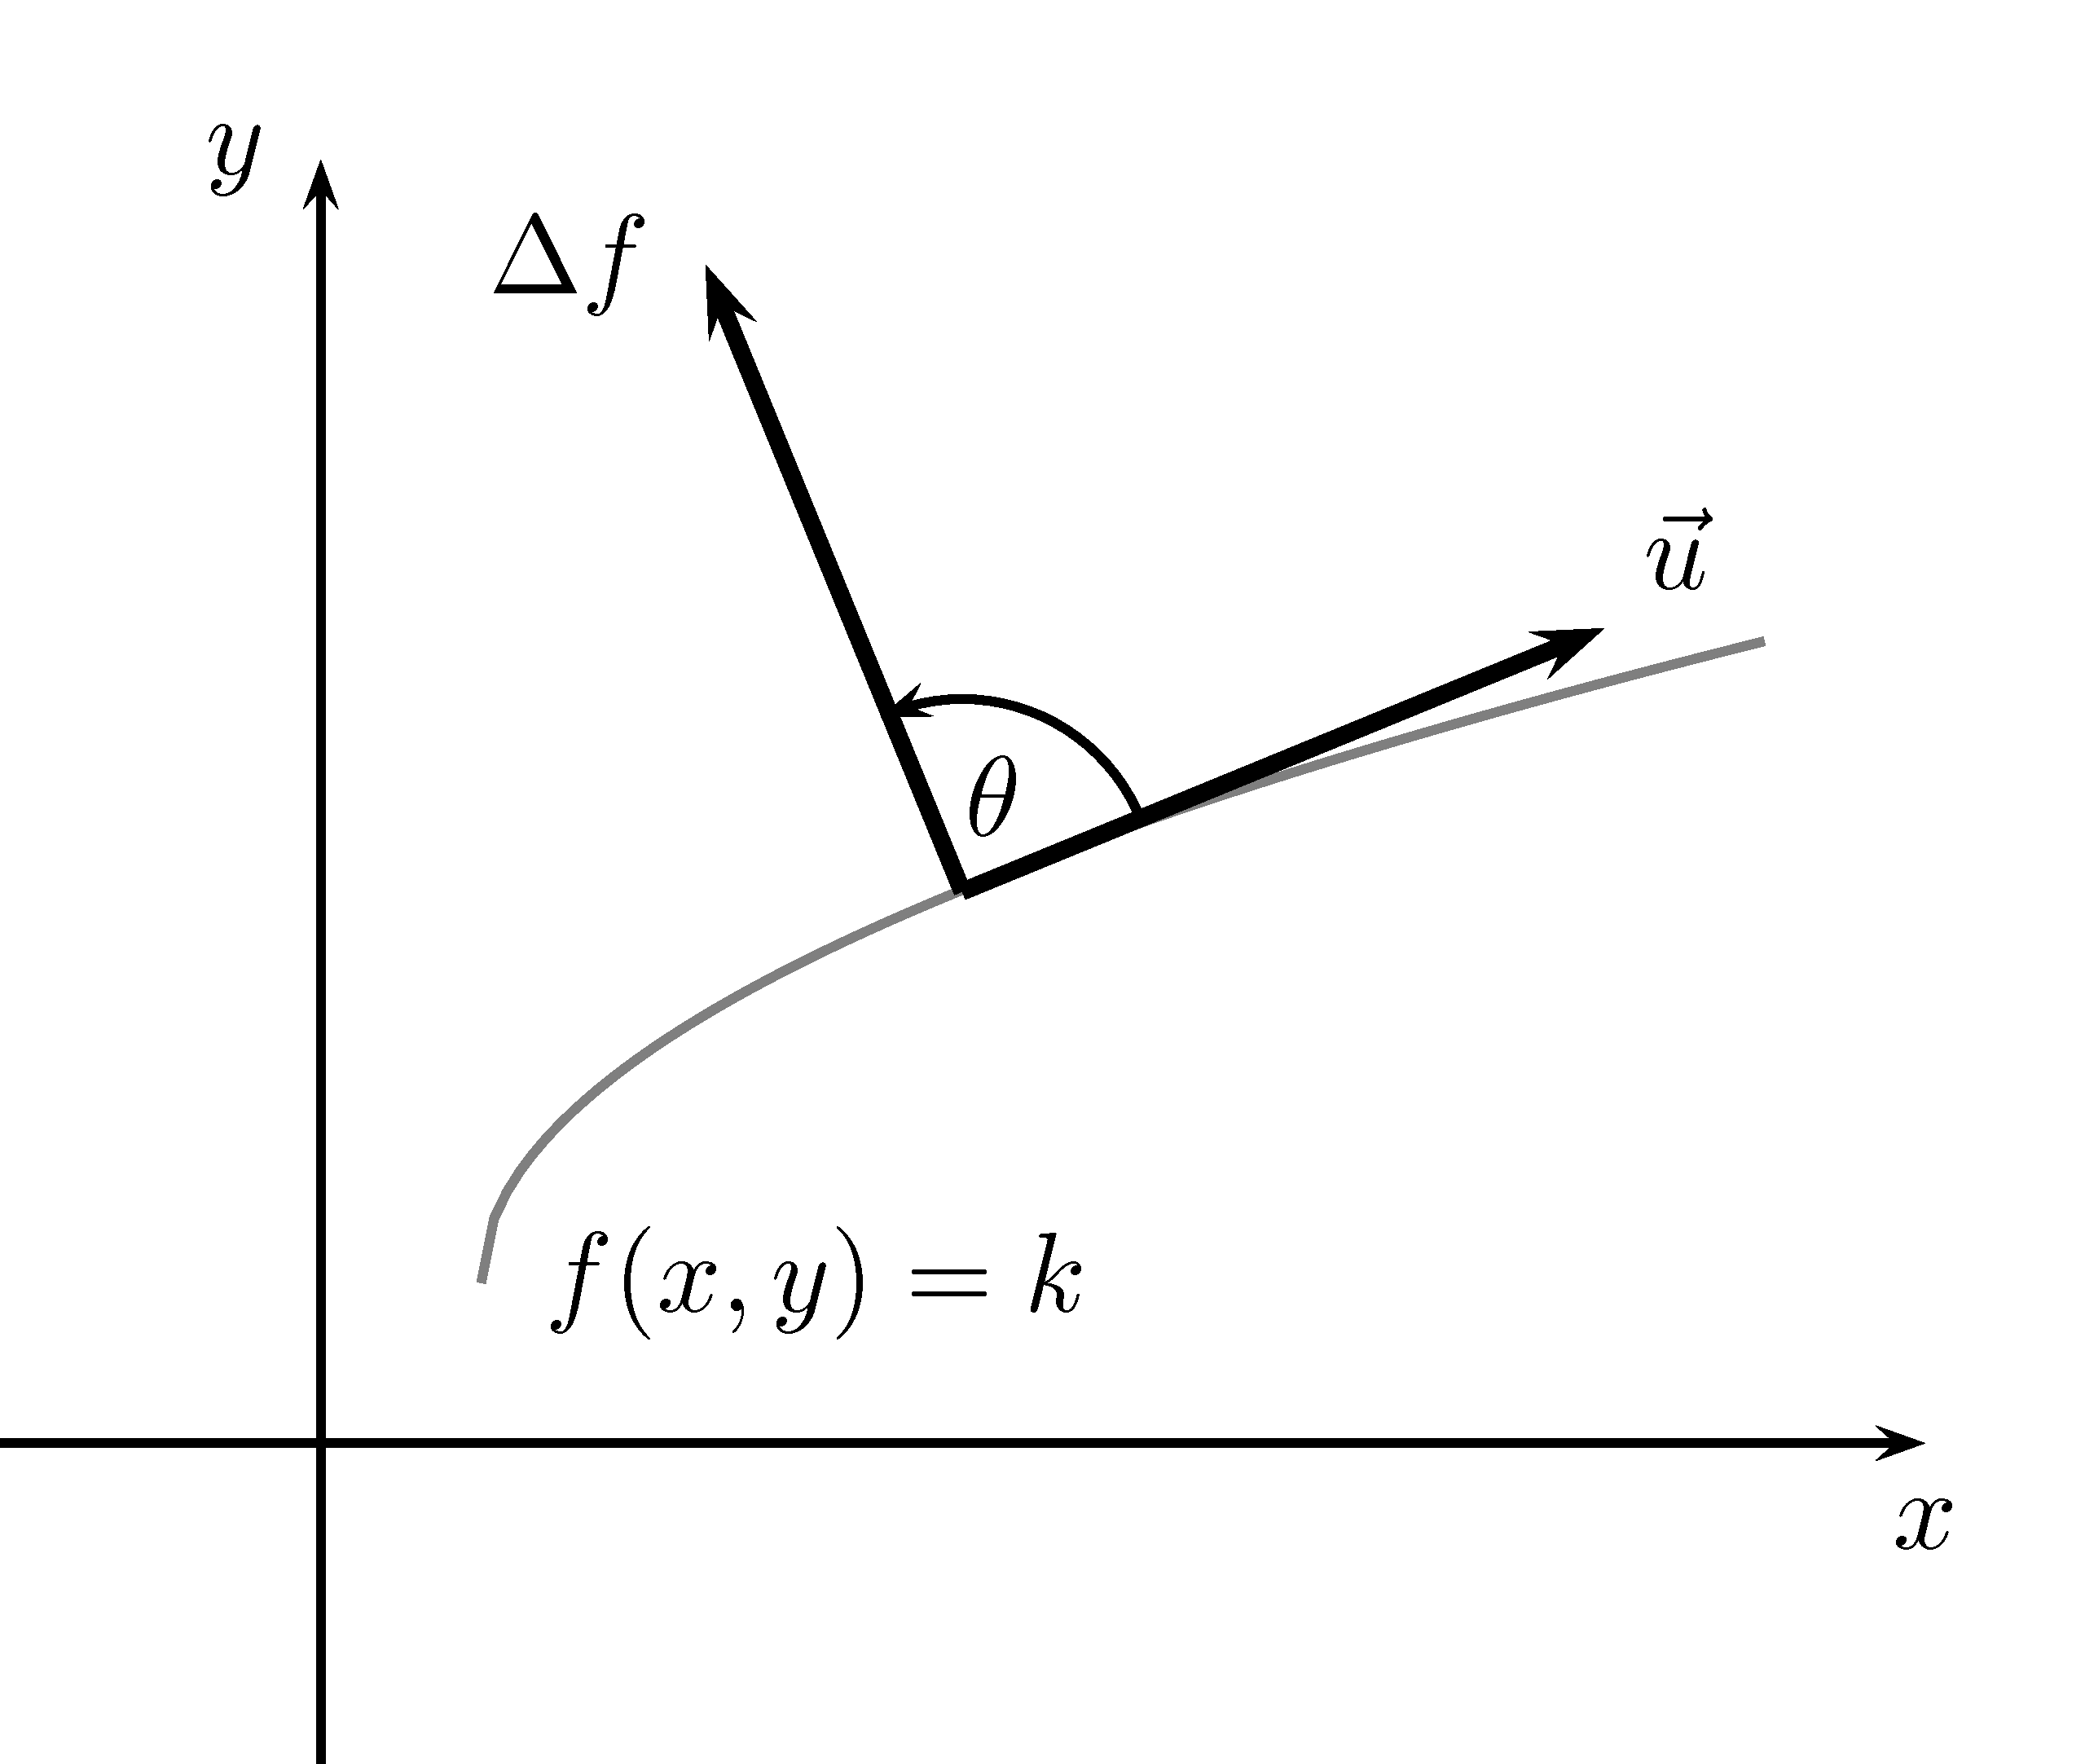
\includegraphics[width=0.5\linewidth]{resources/images/latex/gradientcourbeniveaux} 

}

\caption{Représentation d'une courbe de niveau et du gradient.}\label{fig:gradientcourbeniveaux}
\end{figure}

\hypertarget{le-gradient-des-fonctions-de-plus-de-deux-variables}{%
\subsection{Le gradient des fonctions de plus de deux
variables}\label{le-gradient-des-fonctions-de-plus-de-deux-variables}}

Les notions de dérivée directionnelle et de gradient se généralisent
pour les fonctions de plus de deux variables. Ainsi, si
\(z=f(x_1,x_2,\ldots, x_n)\), nous avons que:

\[ \nabla f = \left[\dfrac{\partial f}{\partial x_1},\dfrac{\partial f}{\partial x_2},\ldots,\dfrac{\partial f}{\partial x_n}\right] \]

Cette généralisation nous permet de simplifier la résolution de certains
problèmes.

\BeginKnitrBlock{example}
\protect\hypertarget{exm:unnamed-chunk-207}{}{\label{exm:unnamed-chunk-207}
}Trouvez l'équation du plan tangent à la surface définie par \(xyz=1\)
en \(x=1\) et \(y=1\).
\EndKnitrBlock{example}
\vspace*{8cm}

\BeginKnitrBlock{example}
\protect\hypertarget{exm:unnamed-chunk-208}{}{\label{exm:unnamed-chunk-208}
}Trouvez l'équation du plan tangent à la surface définie par
\(x^2+y-z^3=1\) en \(x=1\) et \(y=1\).
\EndKnitrBlock{example}
\vspace*{8cm}

\hypertarget{geogebra-derivfctvar}{%
\section{GeoGebra}\label{geogebra-derivfctvar}}

\hypertarget{applet_container}{}

\newpage

\hypertarget{pages-supplementaires-4}{%
\section{Pages supplémentaires}\label{pages-supplementaires-4}}

Des pages blanches supplémentaires pour ajouter, potentiellement, de
nouveaux exemples et exercices.

\multido{\i=1+1}{4}{
\newpage
\mbox{}
}

\hypertarget{optimisation}{%
\chapter{L'optimisation}\label{optimisation}}

Vous trouverez à la section une application
\href{https://www.geogebra.org/?lang=fr}{GeoGebra} vous permettant de
visualiser des coupes transversales et des courbes de niveaux. À noter
que cette application n'est disponible que dans la version en ligne de
ce document.

\hypertarget{introduction-5}{%
\section{Introduction}\label{introduction-5}}

La théorie de l'optimisation des fonctions de plusieurs variables est
très vaste. Nous introduirons ce sujet sans aller trop en profondeur.
Faire de l'optimisation consiste à déterminer les maximums et les
minimums d'une fonction.

\hypertarget{lapproximation-quadratique}{%
\section{L'approximation quadratique}\label{lapproximation-quadratique}}

Nous voulons approcher une fonction \(f(x,y)\) autour d'un point
\((x_0,y_0)\) par un paraboloïde. Ceci correspond à l'analogue de
l'approximation d'une fonction par un polynôme de Taylor de degré 2.
Nous pouvons montrer que le paraboloïde recherché est donné par:

\begin{equation}
\begin{split}
Q(x,y) &= f(x_0,y_0)+f_x(x_0,y_0)(x-x_0)+f_y(y-y_0)+ \\
&\qquad \dfrac{1}{2!}[f_{xx}(x_0,y_0)(x-x_0)^2+2f_{xy}(x_0,y_0)(x-x_0)(y-y_0) \\
& \qquad \qquad +f_{yy}(x_0,y_0)(y-y_0)^2]
\end{split}
\label{eq:approx-quadratique}
\end{equation}

Nous utiliserons l'équation \eqref{eq:approx-quadratique} pour démontrer
la nature des points critiques d'une fonction de deux variables.

\hypertarget{les-points-critiques-et-leur-nature}{%
\section{Les points critiques et leur
nature}\label{les-points-critiques-et-leur-nature}}

\BeginKnitrBlock{definition}
\protect\hypertarget{def:unnamed-chunk-210}{}{\label{def:unnamed-chunk-210}
}Soit une fonction
\(f:D_{\alpha}\subseteq \mathbb{R}^2 \rightarrow \mathbb{R}\). Nous
disons que le point \((x_0,y_0)\) est un point de maximum \textbf{local}
si pour tous les points \((x,y)\) dans le voisinage de \((x_0,y_0)\),
nous avons que: \[ f(x,y) \leq f(x_0,y_0) \] De manière similaire, le
point \((x_0,y_0)\) est un point de minimum \textbf{local} si pour tous
les points \((x,y)\) dans le voisinage de \((x_0,y_0)\), nous avons que:
\[ f(x,y) \geq f(x_0,y_0) \] Le \textbf{maximum absolu} de \(f\) est la
valeur maximale de \(f\) sur \(D\) et le \textbf{minimum absolu} de
\(f\) est la valeur minimale de \(f\) sur \(D\).
\EndKnitrBlock{definition}

\BeginKnitrBlock{theorem}
\protect\hypertarget{thm:gradient-max-min}{}{\label{thm:gradient-max-min}
}Soit une fonction \(z=f(x,y)\) différentiable autour du point
\((x_0,y_0)\). Si le point \((x_0,y_0)\) est un maximum ou minimum local
de \(f\), alors: \[ \nabla f(x_0,y_0)=\overrightarrow{0} \]
\EndKnitrBlock{theorem}

\BeginKnitrBlock{proof}
\iffalse{} {Preuve. } \fi{}Nous savons que si une fonction d'une seule
variable possède un minimum ou un maximum en \(x_0\), alors la dérivée
évaluée en ce point est nulle.

Maintenant, supposons que \((x_0,y_0)\) est un point de maximum (la
démonstration pour le cas d'un minimum est similaire). Si nous fixons
\(x=x_0\), nous avons une fonction d'une seule variable
\(g(y)=f(x_0,y)\). Cette fonction possède un maximum lorsque \(y=y_0\).
Nous avons donc que \(g'(y_0)=0\). Mais \(g'(y_0)=f_y(x_0,y_0)=0\).

D'une manière similaire, nous avons que \(f_x(x_0,y_0)=0\). D'où
\(\nabla f(x_0,y_0)=\overrightarrow{0}\).
\EndKnitrBlock{proof}

\BeginKnitrBlock{remark}
\iffalse{} {Remarque. } \fi{}Il est important de remarquer que le
théorème \ref{thm:gradient-max-min} n'est pas un \textbf{si et seulement
si}. C'est-à-dire que si \((x_0,y_0)\) est un maximum (ou un minimum),
alors le gradient en ce point est nul.

L'inverse n'est pas nécessairement vrai, c'est-à-dire que si le gradient
en un point est nul, il est possible que le point ne soit ni un maximum,
ni un minimum.
\EndKnitrBlock{remark}

Pour spécifier la nature d'un point critique, nous aurons besoin d'un
test supplémentaire.

\BeginKnitrBlock{theorem}
\protect\hypertarget{thm:test-derivee-seconde}{}{\label{thm:test-derivee-seconde}
}Soit une fonction \(z=f(x,y)\) possédant un point critique en
\((x_0,y_0)\). Soit le scalaire:
\[ D=f_{xx}(x_0,y_0)\cdot f_{yy}(x_0,y_0)-\left(f_{xy}(x_0,y_0) \right)^2 \]
Nous pouvons rencontrer les quatres situations suivantes:

\begin{itemize}
\tightlist
\item
  Si \(D>0\) et \(f_{xx}(x_0,y_0)>0\) alors \((x_0,y_0)\) est un point
  de maximum
\item
  Si \(D>0\) et \(f_{xx}(x_0,y_0)<0\) alors \((x_0,y_0)\) est un point
  de minimum
\item
  Si \(D<0\) alors \((x_0,y_0)\) est un point de selle
\item
  Si \(D=0\) alors nous ne pouvons rien conclure
\end{itemize}
\EndKnitrBlock{theorem}

\BeginKnitrBlock{proof}
\iffalse{} {Preuve. } \fi{}Pour simplifier la résolution, nous allons
poser \(A=f_{xx}(x_0,y_0)\), \(B=f_{xy}(x_0,y_0)\) et
\(C=f_{yy}(x_0,y_0)\). Nous allons utiliser l'approximation quadratique
trouvée à l'équation \eqref{eq:approx-quadratique}, pour trouver une
expression pour \(f(x,y)-f(x_0,y_0)\) si \((x,y)\) est près de
\((x_0,y_0)\).

Par l'équation \eqref{eq:approx-quadratique} et puisque
\(f_x(x_0,y_0)=f_y(x_0,y_0)=0\), car \((x_0,y_0)\) est un point
critique, nous avons:
\[ f(x,y)-f(x_0,y_0)=\dfrac{A}{2}(x-x_0)^2+B(x-x_0)(y-y_0)+\dfrac{C}{2}(y-y_0)^2 \]

Ainsi, le signe de \(f(x,y)-f(x_0,y_0)\) sera le même que celui du
membre de droite de l'expression précédente. Nous allons diviser le
membre de droite par \(\dfrac{1}{2}(y-y_0)^2\). Cette division ne
changera pas le signe. Par la suite posons \(w=\dfrac{x-x_0}{y-y_0}\).

Nous obtenons une nouvelle expression, que nous noterons \(E\):
\[ E = Aw^2+2Bw+C \] L'expression \(E\) est un polynôme de degré 2 par
rapport à \(w\). Étudions maintenant le signe de \(E\).

Nous avons que \(E=0\) si:
\[ \dfrac{-2B\pm\sqrt{4B^2-4AC}}{2A}=\dfrac{-B\pm\sqrt{B^2-AC}}{A} \]

Si \(B^2-AC<0\) ou \(D=AC-B^2>0\) alors \(E\) ne possède pas de zéros.
Ceci implique que \(f(x,y)-f(x_0,y_0)\) ne change pas de signe. Ainsi
\(f(x,y)\) est toujours plus grand ou plus petit que \(f(x_0,y_0)\),
pour tout \((x,y)\) près de \((x_0,y_0)\). C'est la définition d'un
maximum ou d'un minimum.

Pour déterminer si nous sommes en présence d'un maximum ou d'un minimum,
nous allons étudier le signe de \(A\). Si \(A<0\), nous avons une
concavité vers le bas, donc un maximum. Si \(A>0\), nous avons une
concavité vers le haut, donc un minimum.

Si \(B^2-AC>0\) ou \(D=AC-B^2<0\), nous avons deux racines et donc
\(f(x,y)-f(x_0,y_0)\) change de signe. C'est ce que nous appelons un
point de selle.
\EndKnitrBlock{proof}

Nous pouvons voir un point de selle en observant la figure
\ref{fig:hyperboloide1}. Le point situé à l'origine est un point de
selle. Dans une direction, la concavité de la fonction est vers le haut
et elle est vers le bas dans l'autre direction.

\begin{figure}

{\centering 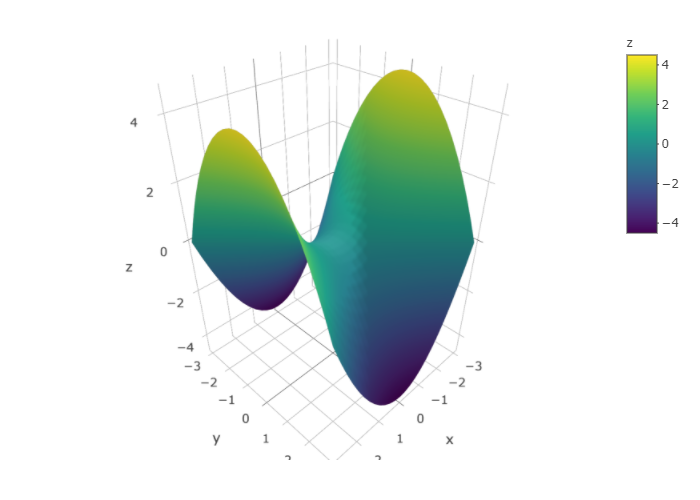
\includegraphics[width=0.8\linewidth]{resources/images/hyperboloide} 

}

\caption{Hyperboloïde : $z=(x^2-y^2)/2$}\label{fig:hyperboloide1}
\end{figure}

\BeginKnitrBlock{example}
\protect\hypertarget{exm:unnamed-chunk-214}{}{\label{exm:unnamed-chunk-214}
}Déterminez tous les points critiques de la fonction \(f(x,y)=x^2-y^2\)
et donnez leur nature.
\EndKnitrBlock{example}
\vspace*{8cm}

\BeginKnitrBlock{example}
\protect\hypertarget{exm:unnamed-chunk-215}{}{\label{exm:unnamed-chunk-215}
}Déterminez tous les points critiques de la fonction
\(f(x,y)=x^4+y^4-4xy+1\) et donnez leur nature.
\EndKnitrBlock{example}
\begin{figure}

{\centering 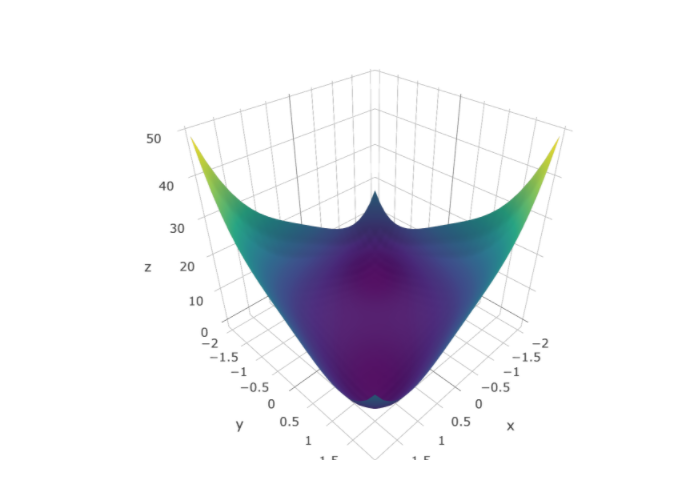
\includegraphics[width=0.8\linewidth]{resources/images/fct_pt_critique} 

}

\caption{Graphique de $f(x,y)=x^4+y^4-4xy+1$}\label{fig:fct-pt-critique}
\end{figure}
\vspace*{8cm}

\BeginKnitrBlock{example}
\protect\hypertarget{exm:unnamed-chunk-216}{}{\label{exm:unnamed-chunk-216}
}Déterminez tous les points critiques de la fonction
\(f(x,y)=2x^3-6xy+3y^2\) et donnez leur nature.
\EndKnitrBlock{example}
\vspace*{8cm}

\BeginKnitrBlock{example}
\protect\hypertarget{exm:unnamed-chunk-217}{}{\label{exm:unnamed-chunk-217}
}Déterminez tous les points critiques de la fonction
\(f(x,y)=xye^{-\frac{x^2+y^2}{2}}\).
\EndKnitrBlock{example}
\vspace*{8cm}

\hypertarget{la-droite-de-regression}{%
\section{La droite de régression}\label{la-droite-de-regression}}

Supposons que nous ayons amassé \(n\) couples de données \((x_i,y_i)\)
pour \(i\in \{1,2,\ldots, n\}\). Nous voulons déterminer l'équation de
laa droite qui minimise la somme des carrés des distances verticales
entre les points et cette droite. En d'autre mots, nous voulons trouver
l'équation de la droite \emph{la plus proche} du nuage de points. Cette
situation est représentée à la figure \ref{fig:droite-regression}.

\begin{figure}

{\centering 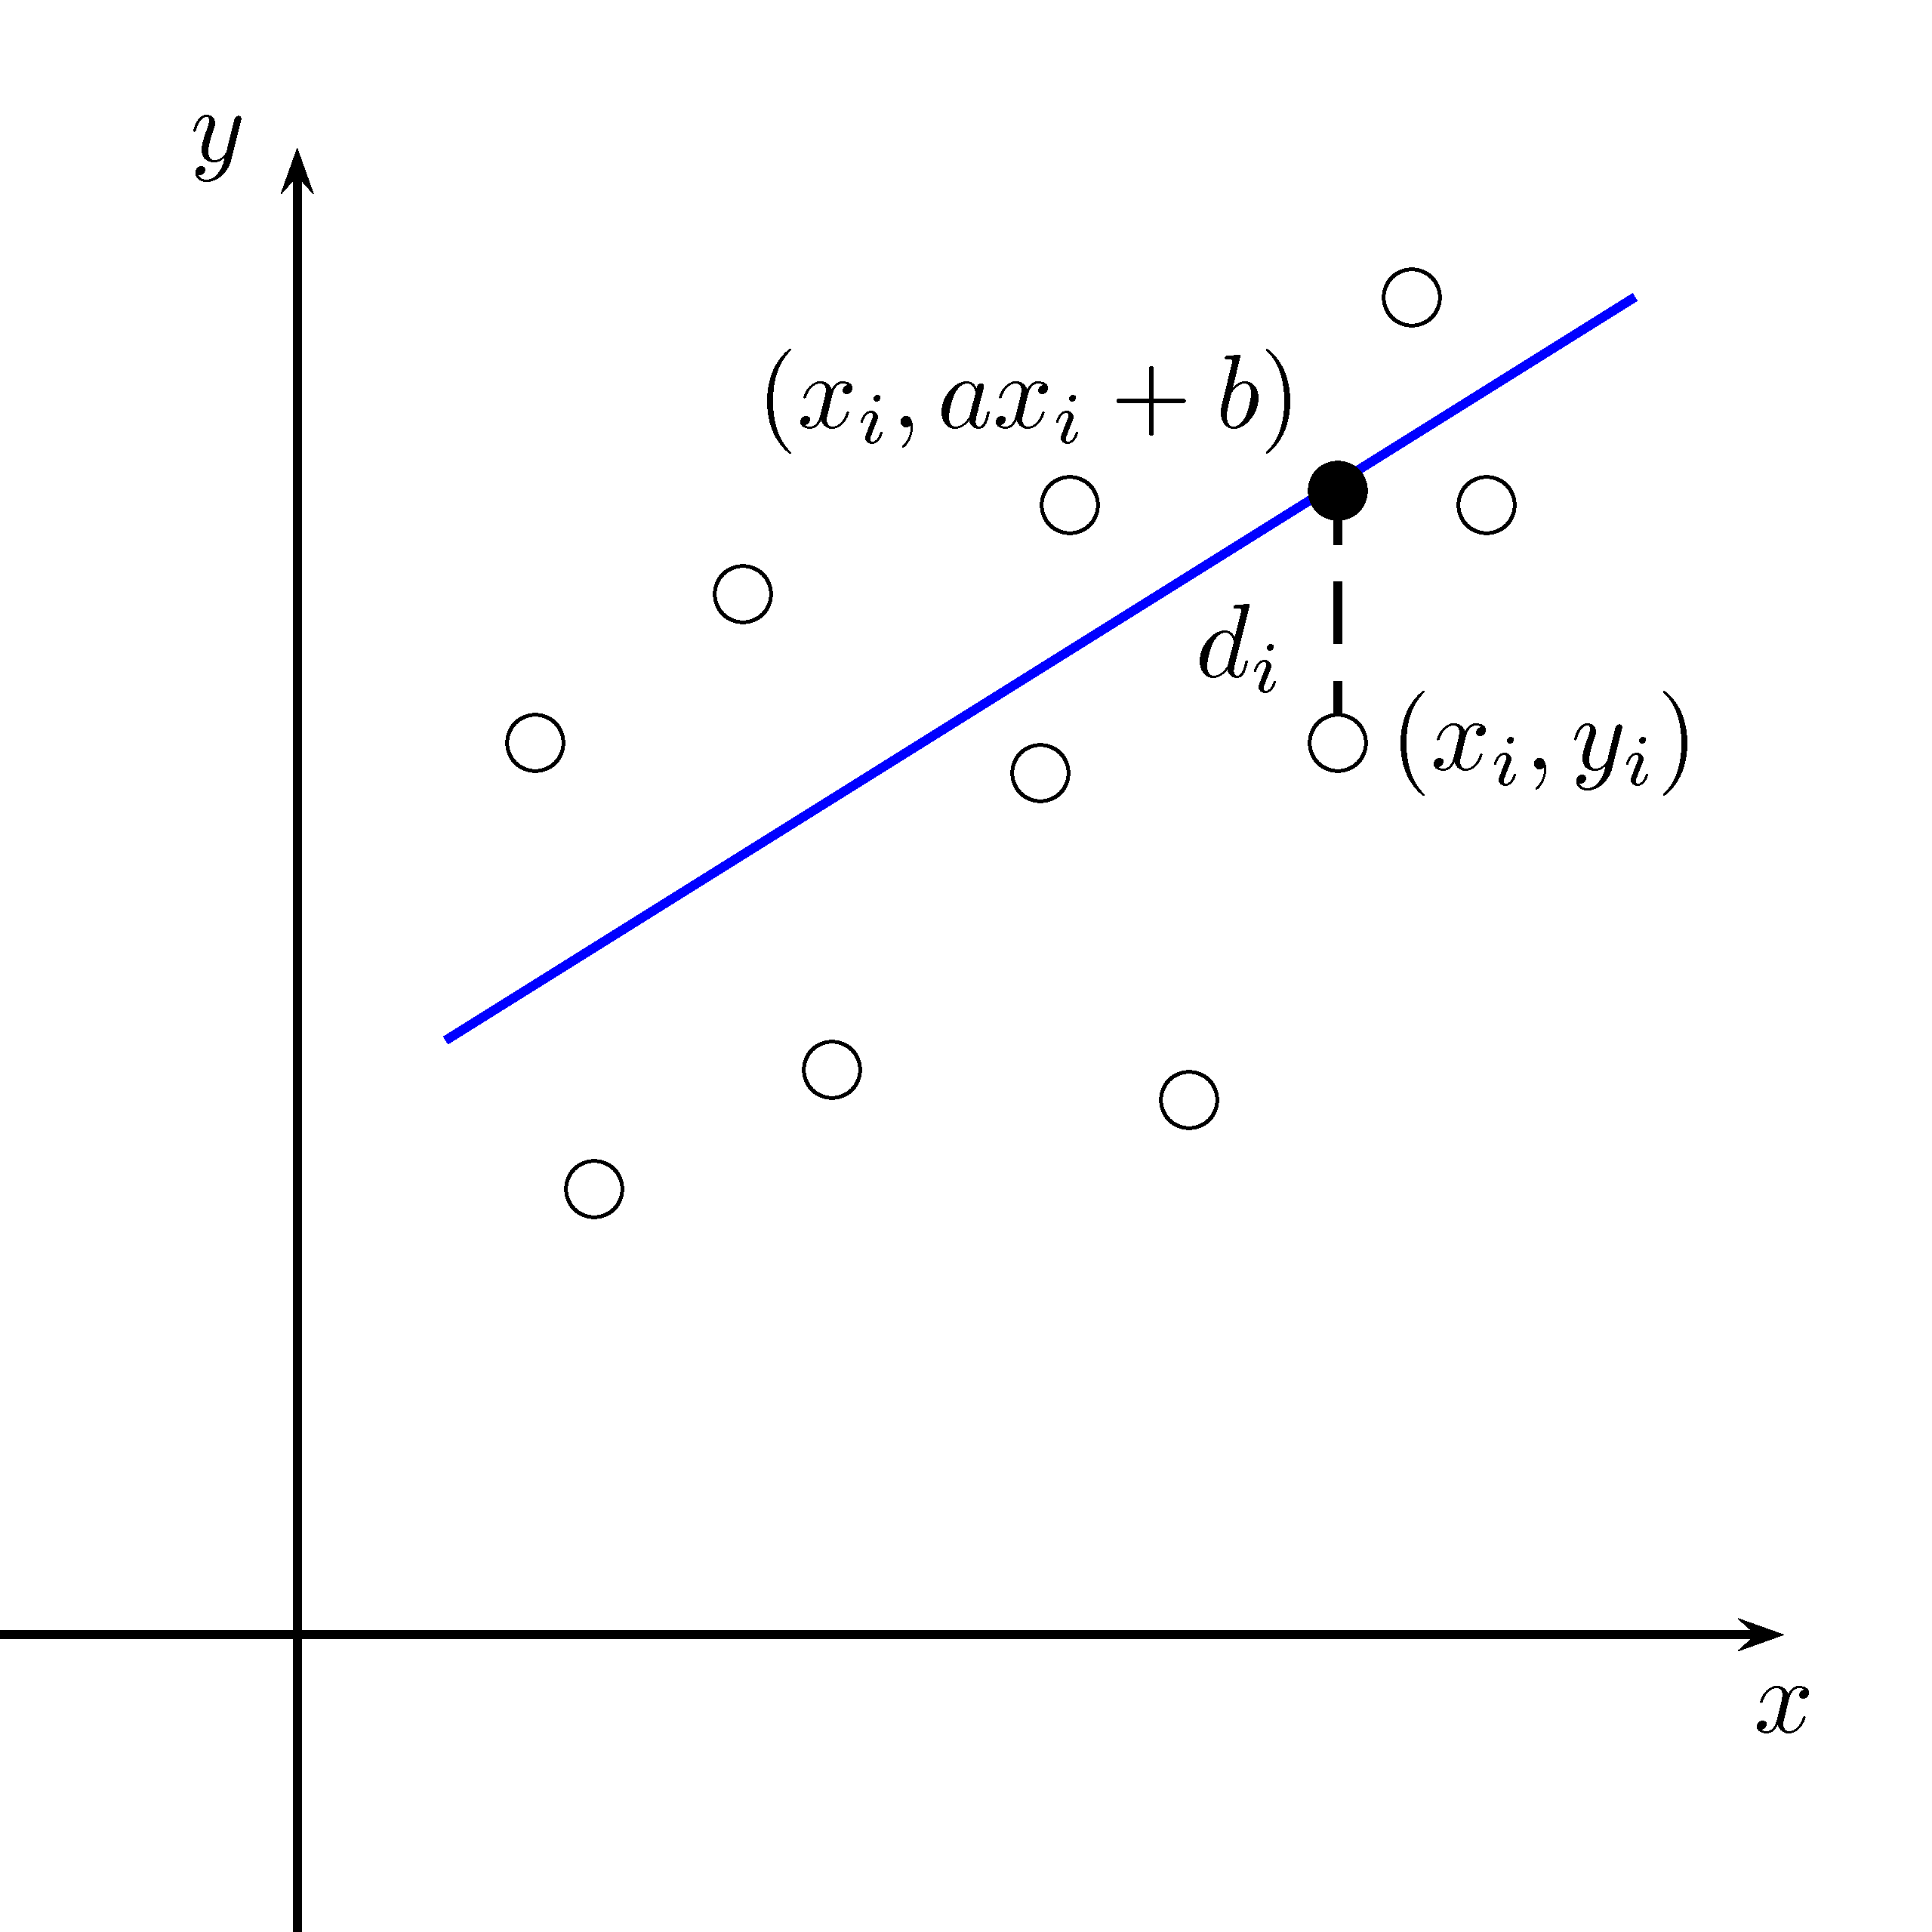
\includegraphics[width=0.5\linewidth]{resources/images/latex/droiteregression} 

}

\caption{Nuage de points et droite de régression}\label{fig:droite-regression}
\end{figure}

Nous allons supposer que l'équation est de la forme \(y=ax+b\) avec
\(a\) et \(b\) que nous devons déterminer en minimisant la somme des
carrés des distances verticales. Nous savons:

\[ d_i^2 = (y-y_i)^2 = (ax_i+b-y_i)^2 \]

Nous voulons minimiser la somme de toutes ces distances, c'est-à-dire:

\begin{equation}
\begin{split}
f(a,b) &= \sum_{i=1}^n d_i^2 \notag \\
&= \sum_{i=1}^n (ax_i+b-y_i)^2
\end{split}
\label{eq:somme-distances}
\end{equation}

Nous désirons trouver \(a\) et \(b\) tels qu'ils minimisent la fonction
\(f(a,b)\). Nous désirons en fait trouver les points critiques de \(f\):

\begin{align}
\dfrac{\partial f}{\partial a} &= \sum_{i=1}^n 2x_i(ax_i+b-y_i) = 0 \label{eq:deriv1}\\
\dfrac{\partial f}{\partial b} &= \sum_{i=1}^n 2(ax_i+b-y_i) = 0 \label{eq:deriv2}
\end{align}

En utilisant l'équation \eqref{eq:deriv2}, nous obtenons:

\begin{align}
\sum_{i=1}^n 2(ax_i+b-y_i) &= 0 \notag\\
\sum_{i=1}^n 2ax_i + \sum_{i=1}^n 2b - \sum_{i=1}^n 2y_i &= 0 \notag\\
b \sum_{i=1}^n 1 &= \sum_{i=1}^n y_i - a \sum_{i=1}^n x_i \notag\\
bn &= \sum_{i=1}^n y_i - a \sum_{i=1}^n x_i \notag\\
b &= \dfrac{\sum\limits_{i=1}^n y_i - a \sum\limits_{i=1}^n x_i}{n} \label{eq:valeurb}
\end{align}

Nous devons maintenant remplacer l'équation \eqref{eq:valeurb} dans
l'équation \eqref{eq:deriv1}.

\begin{align*}
\sum_{i=1}^n 2x_i(ax_i+b-y_i) &= 0 \\
a\sum_{i=1}^n x_i^2 + b \sum_{i=1}^n x_i - \sum_{i=1}^n x_iy_i &= 0 \\
a\sum_{i=1}^n x_i^2 + \left(\dfrac{\sum\limits_{i=1}^n y_i - a \sum\limits_{i=1}^n x_i}{n}\right) \sum_{i=1}^n x_i - \sum_{i=1}^n x_iy_i &= 0 \\
an\sum_{i=1}^n x_i^2+\left(\sum_{i=1}^n x_i\right)\left(\sum_{i=1}^n y_i\right)-a\left(\sum_{i=1}^n x_i\right)^2- \sum_{i=1}^n x_iy_i &= 0 \\
a\left(n\sum_{i=1}^n x_i^2-\left(\sum_{i=1}^n x_i\right)^2\right) &= \sum_{i=1}^n x_iy_i-\left(\sum_{i=1}^n x_i\right)\left(\sum_{i=1}^n y_i\right) \\
a &= \dfrac{\sum\limits_{i=1}^n x_iy_i-\left(\sum\limits_{i=1}^n x_i\right)\left(\sum\limits_{i=1}^n y_i\right)}{n\sum\limits_{i=1}^n x_i^2-\left(\sum\limits_{i=1}^n x_i\right)^2}
\end{align*}

En résumé, nous avons:

\begin{align*}
a &= \dfrac{\sum\limits_{i=1}^n x_iy_i-\left(\sum\limits_{i=1}^n x_i\right)\left(\sum\limits_{i=1}^n y_i\right)}{n\sum\limits_{i=1}^n x_i^2-\left(\sum\limits_{i=1}^n x_i\right)^2} \\
b &= \dfrac{\sum\limits_{i=1}^n y_i - a \sum\limits_{i=1}^n x_i}{n}
\end{align*}

En utilisant le théorème \ref{thm:test-derivee-seconde}, nous pourrions
démontrer que ces valeurs de \(a\) et \(b\) minimisent la fonction
\(f\).

\BeginKnitrBlock{example}
\protect\hypertarget{exm:unnamed-chunk-218}{}{\label{exm:unnamed-chunk-218}
}Utilisez les données suivantes pour trouver la droite de régression
associée au nuage de points de la figure \ref{fig:anscombe1}.
\EndKnitrBlock{example}

\begin{tabular}{cc}
\toprule
x & y\\
\midrule
10 & 8.04\\
8 & 6.95\\
13 & 7.58\\
9 & 8.81\\
11 & 8.33\\
\addlinespace
14 & 9.96\\
6 & 7.24\\
4 & 4.26\\
12 & 10.84\\
7 & 4.82\\
\addlinespace
5 & 5.68\\
\bottomrule
\end{tabular}

\begin{figure}

{\centering 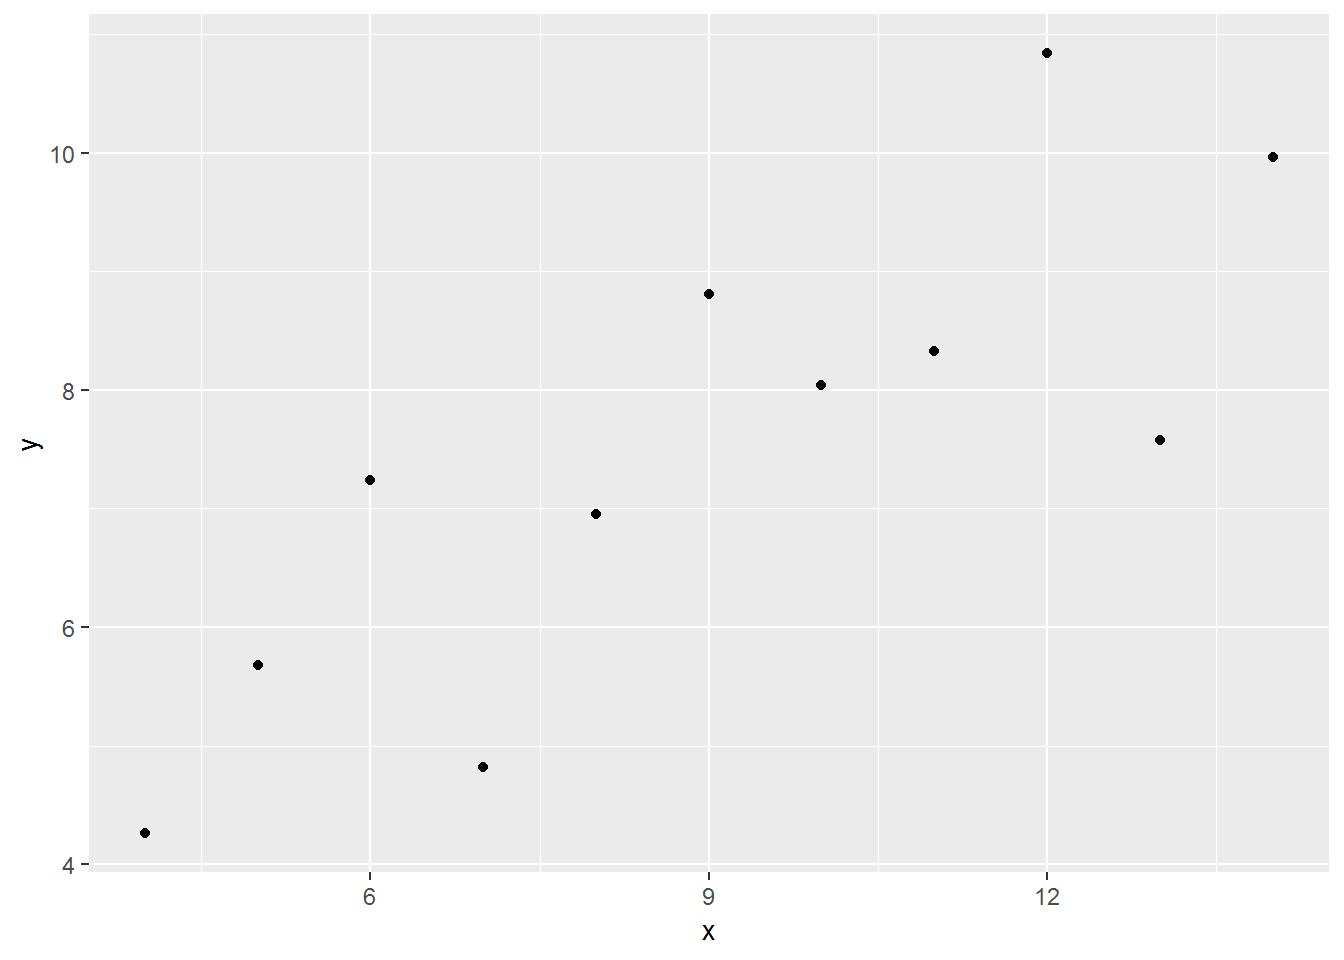
\includegraphics{calcul3_files/figure-latex/anscombe1-1} 

}

\caption{Le nuage de points.}\label{fig:anscombe1}
\end{figure}
\vspace*{10cm}

\hypertarget{le-quartet-danscombe}{%
\subsection{Le quartet d'Anscombe}\label{le-quartet-danscombe}}

Le quartet d'Anscombe est constitué de quatre ensembles de données qui
ont les mêmes propriétés statistiques simples mais qui sont en réalité
très différents, ce qui se voit facilement lorsqu'on les représente sous
forme de graphiques. Ils ont été construits en 1973 par le statisticien
Francis Anscombe dans le but de démontrer l'importance de tracer des
graphiques avant d'analyser des données, car cela permet notamment
d'estimer l'incidence des données aberrantes sur les différentes indices
statistiques que l'on pourrait calculer.

Dans la table \ref{tab:quartet-anscombe}, les observations \(x_i\) sont
reliées aux observations \(y_i\).

\begin{table}[t]

\caption{\label{tab:quartet-anscombe}Le quartet d'Anscombe}
\centering
\begin{tabular}{cccccccc}
\toprule
x1 & x2 & x3 & x4 & y1 & y2 & y3 & y4\\
\midrule
10 & 10 & 10 & 8 & 8.04 & 9.14 & 7.46 & 6.58\\
8 & 8 & 8 & 8 & 6.95 & 8.14 & 6.77 & 5.76\\
13 & 13 & 13 & 8 & 7.58 & 8.74 & 12.74 & 7.71\\
9 & 9 & 9 & 8 & 8.81 & 8.77 & 7.11 & 8.84\\
11 & 11 & 11 & 8 & 8.33 & 9.26 & 7.81 & 8.47\\
\addlinespace
14 & 14 & 14 & 8 & 9.96 & 8.10 & 8.84 & 7.04\\
6 & 6 & 6 & 8 & 7.24 & 6.13 & 6.08 & 5.25\\
4 & 4 & 4 & 19 & 4.26 & 3.10 & 5.39 & 12.50\\
12 & 12 & 12 & 8 & 10.84 & 9.13 & 8.15 & 5.56\\
7 & 7 & 7 & 8 & 4.82 & 7.26 & 6.42 & 7.91\\
\addlinespace
5 & 5 & 5 & 8 & 5.68 & 4.74 & 5.73 & 6.89\\
\bottomrule
\end{tabular}
\end{table}

Avant d'afficher les ensembles de données, nous allons calculer quelques
mesures sur chacun de ces ensembles, à savoir, la moyenne des \(x\), la
moyenne des \(y\), la variance des \(x\), la variance des \(y\) et le
coefficient de corrélation.

\begin{tabular}{c|c|c|c|c|c}
\hline
ensemble & moyenne des \$x\$ & variance des \$x\$ & moyenne des \$y\$ & variance des \$y\$ & coeff. de corrélation\\
\hline
I & 9 & 11 & 7.500909 & 4.127269 & 0.8164205\\
\hline
II & 9 & 11 & 7.500909 & 4.127629 & 0.8162365\\
\hline
III & 9 & 11 & 7.500000 & 4.122620 & 0.8162867\\
\hline
IV & 9 & 11 & 7.500909 & 4.123249 & 0.8165214\\
\hline
\end{tabular}

Comme nous pouvons le remarquer, les quatre ensembles de données
possèdent les mêmes mesures. Par contre, lorsque nous affichons ensuite
les quatre ensembles de données, nous remarquons que ces ensembles sont
très différents.

\begin{figure}

{\centering 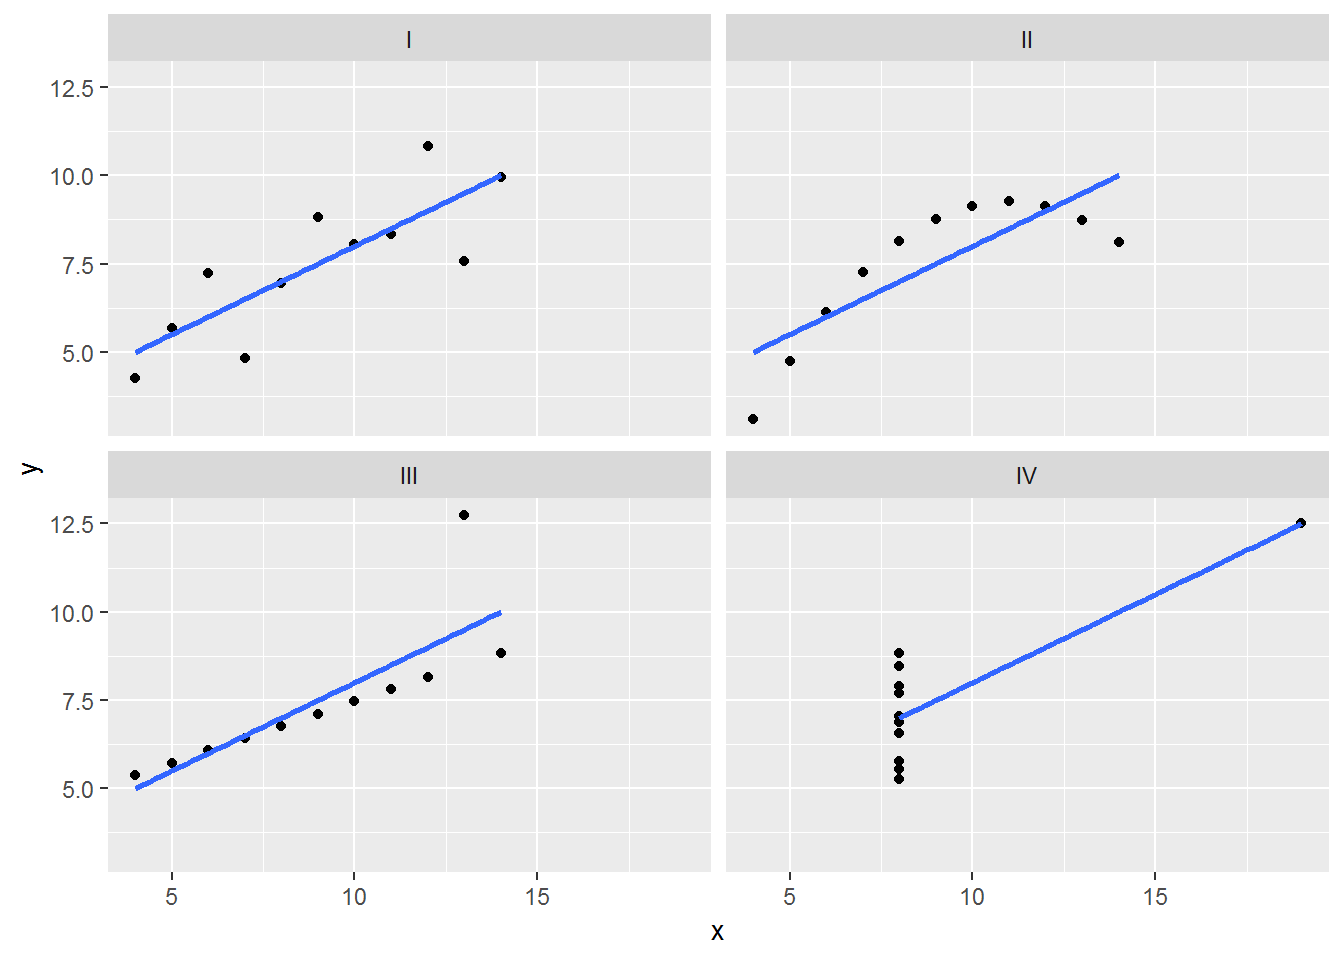
\includegraphics{calcul3_files/figure-latex/graphe-quartet-anscombe-1} 

}

\caption{Les nuages de points et les droites de régression pour le quartet d'Anscombe.}\label{fig:graphe-quartet-anscombe}
\end{figure}

\hypertarget{datasaurus}{%
\subsection{DatasauRus}\label{datasaurus}}

Les données disponibles dans la librairie \texttt{datasauRus} nous
montrent pourquoi la visualisation est importante. Les treize ensembles
de données possèdent tous les mêmes statiistiques descriptives et les
mêmes droites de régression, mais leur aspect graphique est fort
différent.

La table \ref{tab:datasaurus-mesures} montre les mesures pour les treize
ensembles de données.

\begin{table}[t]

\caption{\label{tab:datasaurus-mesures}Les mesures de datasauRus}
\centering
\begin{tabular}{cccccc}
\toprule
dataset & moyenne des \$x\$ & variance des \$x\$ & moyenne des \$y\$ & variance des \$y\$ & coeff. de corrélation\\
\midrule
away & 54.26610 & 281.2270 & 47.83472 & 725.7498 & -0.0641284\\
bullseye & 54.26873 & 281.2074 & 47.83082 & 725.5334 & -0.0685864\\
circle & 54.26732 & 280.8980 & 47.83772 & 725.2268 & -0.0683434\\
dino & 54.26327 & 281.0700 & 47.83225 & 725.5160 & -0.0644719\\
dots & 54.26030 & 281.1570 & 47.83983 & 725.2352 & -0.0603414\\
\addlinespace
h\_lines & 54.26144 & 281.0953 & 47.83025 & 725.7569 & -0.0617148\\
high\_lines & 54.26881 & 281.1224 & 47.83545 & 725.7635 & -0.0685042\\
slant\_down & 54.26785 & 281.1242 & 47.83590 & 725.5537 & -0.0689797\\
slant\_up & 54.26588 & 281.1944 & 47.83150 & 725.6886 & -0.0686092\\
star & 54.26734 & 281.1980 & 47.83955 & 725.2397 & -0.0629611\\
\addlinespace
v\_lines & 54.26993 & 281.2315 & 47.83699 & 725.6388 & -0.0694456\\
wide\_lines & 54.26692 & 281.2329 & 47.83160 & 725.6506 & -0.0665752\\
x\_shape & 54.26015 & 281.2315 & 47.83972 & 725.2250 & -0.0655833\\
\bottomrule
\end{tabular}
\end{table}

La figure \ref{fig:datasaurus-graph} représente les 13 ensembles de
données graphiquement avec leurs droites de régression.

\begin{figure}

{\centering 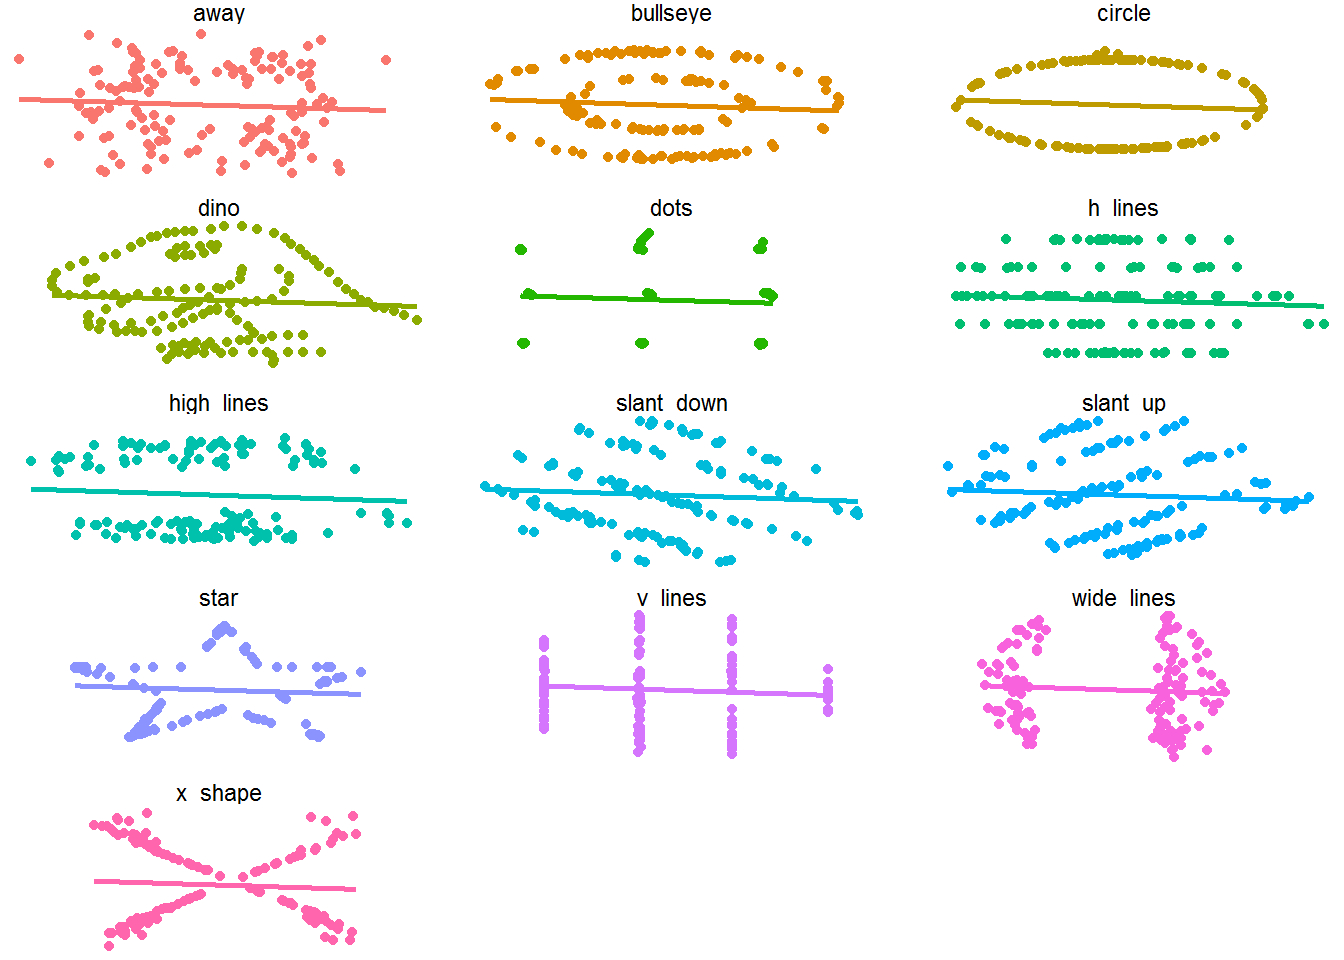
\includegraphics{calcul3_files/figure-latex/datasaurus-graph-1} 

}

\caption{Les 13 ensembles de données de datasauRus.}\label{fig:datasaurus-graph}
\end{figure}

\hypertarget{dautres-types-de-regression}{%
\subsection{D'autres types de
régression}\label{dautres-types-de-regression}}

TODO\ldots{} MAYBE

\hypertarget{la-distance-minimale}{%
\section{La distance minimale}\label{la-distance-minimale}}

La distance entre deux objets mathématiques (points, droites, plans,
\ldots{}) correspond en réalité à la plus petite distance entre ces
objets. Pour trouver cette plus courte distance, nous utiliserons
l'optimisation des fonctions de plusieurs variables.

\BeginKnitrBlock{remark}
\iffalse{} {Remarque. } \fi{}Habituellement, nous minimiserons le carré
de la distance plutôt que la distance. Nous obtenons de cette façon le
même résultat mais les calculs à faire seront plus simples.
\EndKnitrBlock{remark}

\BeginKnitrBlock{example}
\protect\hypertarget{exm:unnamed-chunk-223}{}{\label{exm:unnamed-chunk-223}
}Trouvez la distance entre le point \((1,2,3)\) et le plan \(x+y+z=1\).
\EndKnitrBlock{example}
\vspace*{8cm}

\hypertarget{loptimisation-avec-contraintes}{%
\section{L'optimisation avec
contraintes}\label{loptimisation-avec-contraintes}}

Jusqu'à maintenant, nous avons optimisé des fonctions sans contraintes,
c'est-à-dire que nous optimisions la fonction sur tout son domaine. Par
contre, nous devons parfois optimiser une fonction sur un ensemble fermé
de \(\mathbb{R}^2\).

Le théorème des valeurs extrèmes pour les fonctions d'une seule variable
stipule que si \(f\) est continue sur un intervalle fermé \([a,b]\),
alors \(f\) atteint un minimum absolu et un maximum absolu.

La situation est semblable pour les fonctions de deux variables.

\BeginKnitrBlock{definition}[Ensemble fermé]
\protect\hypertarget{def:unnamed-chunk-224}{}{\label{def:unnamed-chunk-224}
\iffalse (Ensemble fermé) \fi{} }Un ensemble fermé de \(\mathbb{R}^2\)
est un ensemble qui contient ses points frontières.
\EndKnitrBlock{definition}

Par exemple, le disque \(D=\{(x,y)\in\mathbb{R}^2\mid x^2+y^2\leq 1\}\)
composé de tous les points à l'intérieur du cercle \(x^2+y^2=1\) et de
tous les points sur le cercle.

\BeginKnitrBlock{definition}[Ensemble borné]
\protect\hypertarget{def:unnamed-chunk-225}{}{\label{def:unnamed-chunk-225}
\iffalse (Ensemble borné) \fi{} }Un ensemble borné de \(\mathbb{R}^2\)
est un ensemble contenu dans un certain disque. Il est donc d'étendue
finie.
\EndKnitrBlock{definition}

\BeginKnitrBlock{theorem}[Théorème des valeurs extrèmes pour les fonctions de deux variables]
\protect\hypertarget{thm:valeurs-extremes}{}{\label{thm:valeurs-extremes}
\iffalse (Théorème des valeurs extrèmes pour les fonctions de deux
variables) \fi{} }Si \(f(x,y)\) est une fonction continue sur un
ensemble borné et fermé \(D\) de \(\mathbb{R}^2\), alors \(f\) atteint
un maximum absolu \(f(x_1,y_1)\) et un minimum absolu \(f(x_2,y_2)\) en
des points \((x_1,y_1)\) et \((x_2,y_2)\) de \(D\).
\EndKnitrBlock{theorem}

Pour déterminer les valeurs extrèmes d'une fonction continue \(f(x,y)\)
sur un ensemble borné fermé \(D\), dont l'existence est garantie par le
théorème \ref{thm:valeurs-extremes}, les étapes sont les suivantes:

\begin{enumerate}
\def\labelenumi{\arabic{enumi}.}
\item
  Calculez les valeurs de \(f\) aux points critiques de \(f\) dans
  \(D\);
\item
  Calculez les valeurs extrèmes de \(f\) sur la frontière de \(D\);
\item
  La plus grande des valeurs des étapes \(1\) et \(2\) est la valeur
  maximale absolue, la plus petite de ces valeurs est la valeur minimale
  absolue.
\end{enumerate}

\BeginKnitrBlock{example}
\protect\hypertarget{exm:unnamed-chunk-226}{}{\label{exm:unnamed-chunk-226}
}Trouvez les valeurs extrèmes absolues de la fonction
\(f(x,y)=x^2-2xy+2y\) sur le rectangle
\[ D=\{(x,y)\in\mathbb{R}^2 \mid 0 \leq x \leq 3, 0 \leq y \leq 2 \} \]
\EndKnitrBlock{example}
\begin{figure}

{\centering 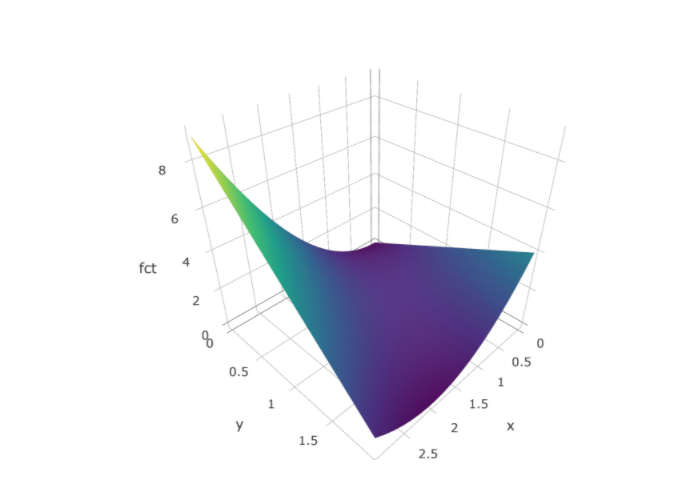
\includegraphics[width=0.8\linewidth]{resources/images/optim_rect} 

}

\caption{La fonction $f(x,y)=x^2-2xy+2y$}\label{fig:optimisation-rectangle}
\end{figure}

\hypertarget{intfctvars}{%
\chapter{L'intégration de fonctions de plusieurs
variables}\label{intfctvars}}

\bibliography{book.bib,packages.bib}


\end{document}
